\section{Application to mechanical systems}
\label{sec:mechanical}
We will now proceed by using a mechanical `prototype' example for our mechanical system: the harmonic oscillator with \emph{two} dampers: one in series and one in parallel, as discussed in \cref{ssec:serial_damping}. We consider a system with two dampers because the corresponding state transition matrix is completely `filled': as such, this system can represent all the possible two-dimensional systems discussed in the previous section. %Furthermore, the two dampers have a very distinctive interpretation within the field of economic engineering.

\subsection{Equations of motion}
The harmonic oscillator with two dampers is shown in \cref{fig:double_damped_osc}. 
%The equations of motion can be readily derived:
%\begin{equation}
%    \begin{split}
%        m\ddot{q}_1 &= -kq - b_p \dot{q}_1 \\
%        kq &= b_s(\dot{q}_1 - \dot{q}) \\
%    \end{split}
%\end{equation}
%Due to the presence of the serial damper, the situation is somewhat curious, since there are two positions in the system; one measuring the spring deflection $q$ and the position of the mass $q_1$. However, the node connecting the serial damper and the spring has no mass, and therefore no second-order dynamics: as such, the overall order of the system is 2. In accordance with the economic analogy, we will say that position is stored in the spring, but momentum is stored in a mass. Hence, let $p = m\dot{q}_1$ --- but $\dot{q} \neq p/m$ in general. 
The equations of motion of the harmonic oscillator with parallel and serial damping are given in \cref{eq:serial_eom_raw}. In matrix form, we have:
\begin{equation*}
    \mqty(\dot{q}\\\dot{p}) = \mqty(-\tfrac{k}{b_s} & \tfrac{1}{m} \\ -k & - \tfrac{b_p}{m})\mqty(q \\ p),
\end{equation*}
or, using the parameters defined in \cref{tab:ddho_params}:
\begin{equation}
    \mqty(\dot{q}\\\dot{p}) = \underbrace{\mqty(-\gamma_s & \frac{1}{m} \\ -m\Omega_n^2 & - \gamma_p)}_A \mqty(q \\ p).
    \label{eq:ddho_eom}
\end{equation}
%The nontrivial relation between momentum and the $\dot{q}$ also precludes us from casting this system directly to the Lagrangian formalism, because the vector field is not second-order. A second-order vector field implies that the `velocities' really are the time derivatives of the `positions', (cf. \cref{app:symplectic_geometry} for a more formal discussion).
%\begin{table}[ht!]
%    \caption{Substition parameters for the harmonic oscillator with serial and parallel damping, shown in \cref{fig:double_damped_osc}.}
%    \label{tab:ddho_params}
%    \centering
%    \begin{tabular}{llll}
%        \toprule
%        \textbf{Name} & \textbf{Symbol} & \textbf{Value} & \textbf{Units} \\
%        \midrule
%            Serial damping coefficient & $\gamma_s$ & $k/b_s$ & \si{\per \second} \\
%            Parallel damping coefficient & $\gamma_p$ & $b_p/m$ & \si{\per \second} \\
%            Natural frequency & $\Omega_n$ & $\sqrt{k/m}$ & \si{\per \second} \\
%            Damped frequency & $\Omega_d$ &  & \si{\per \second} \\
%        \bottomrule
%    \end{tabular}
%\end{table}

The split-quaternion associated with the $A$-matrix of the doubly damped system can easily be found using the mapping defined by \cref{eq:inv_quat_isom}. We must, however, be careful when dealing with physical systems, because the entries of the $A$-matrix are not dimensionless. In a vector space, we associate the units with the basis vectors, not with the components. For example, in a two-dimensional vector space spanned by a axis for apples and and an axis for pears, and we wish to represent that someone possesses three apples and four pairs, the \emph{components} of that vector are $(3, 4)$, and the \emph{unit vectors} are $(1 \text{ apple}, 1\text{ pear})$. Along the same line, we must define the units in the $A$-matrix in the split-quaternion basis elements 1, \quati, \quatj, \quatk. To do so, we define the reference quantities and $m_0, t_0$. The basis elements are then mapped in terms of these reference quantities:
$$ 
    \phi(1) = \mqty(\tfrac{1}{t_0} & 0 \\ 0 & \tfrac{1}{t_0}), \quad 
    \phi(\quati) = \mqty(0 & \tfrac{1}{m_0} \\  -\tfrac{m_0}{t_0^2} & 0), \quad
    \phi(\quati) = \mqty(0 & \tfrac{1}{m_0} \\  \tfrac{m_0}{t_0^2} & 0), \quad
    \phi(\quatk) = \mqty(\tfrac{1}{t_0} & 0 \\ 0 & -\tfrac{1}{t_0}), \quad 
$$
where, in case we would use SI units, $m_0 = \SI{1}{\kilogram}$ and $t_0 = \SI{1}{\second}$. As a result, the split-quaternion associated with the $A$-matrix given in \cref{eq:ddho_eom} becomes
\begin{equation}
    a\:=\: -\frac{1}{2}\qty(t_0\gamma_s + t_0\gamma_p)\:+\:\frac{1}{2}\qty(\frac{m_0}{m} + \frac{m\Omega_n^2 t_0^2}{m_0})\quati\:+\:\frac{1}{2}\qty(\frac{m_0}{m} + \frac{m\Omega_n^2 t_0^2}{m_0})\quatj\:+\:\frac{1}{2}\qty(t_0\gamma_p - t_0\gamma_s)\quatk. 
    \label{eq:ddho_quat_units}
\end{equation}
Clearly, all the components of the split-quaternion are dimensionless. This really is not too wild of an idea: after all, we are translating the matrix itself, and \emph{not} the two-dimensional vector space that it acts on. The units are inherited from the vector space, so we should only add them when returning from the split-quaterions back to the realm of the matrices. 

The preceding argument only explains why we can work around this issue without performing illegal operations, but it does not give a satisfactory answer as to why we would be interested to add numbers that are seemingly incompatible. Indeed, observe that $\gamma_s$ and $\gamma_p$ have the same units, whereas $\tfrac{1}{m}$ and $\Omega_n^2$ do not. So, in which sense can the $\quati$ and $\quatj$-components be of any signficance? To answer this question, we first note that `rescaling of units' is a linear operation on the vector space given by a diagonal matrix (with nonzero diagonal entries): 
$$ N = \mqty(\dmat[0]{\nu_1}{\nu_2}) \qquad \nu_1, \nu_2 \in \real^*, $$
which form the group isomorphic to $(\real^*)^2$. This transformation of the vector space manifests itself on the $A$-matrix as: $ A' = N^{-1}A N$. It is easy to see that the basis matrices (or vector fields) for `1' and \quatk are invariant under this transformation, while the \quati and \quatj-matrices are not (that is, without making use of the reference quantities). 

A geometric explanation is that the eigenvectors of the identity matrix and the \quatk-matrix point along the axes; and are therefore invariant under rescaling of these axes. As a result of this fact, the \quati and \quatj components will not transform properly under a unit transformation. It is common practice in physics to rescale the state space of the undamped harmonic oscillator as follows \cite{Dekker1981,Dedene1980}
$$ p \mapsto \frac{p}{m} \qquad q \mapsto m\Omega q, $$
such that the Hamiltonian reverts to a particularly convenient form. We can see that this is precisely the transformation that kills the \quatj-component of the split-quaternion. This would essentially resolve this `unit problem', because it only arises when we attempt to make the \emph{distinction} between the \quati and \quatj-component.

In contrast to common practice in physics, we are interested in the full range of geometrical properties that the trajectories in the phase plane can exhibit, including those that are not invariant under the action of the structure group $(\real^*)^2$ that contains the changes of units. Furthermore, many invariants, such as the split-quaternion (vector) norm, scalar part, etc. that we use to draw conclusions about the nature of the system \emph{do} commute with this group action, and are therefore remain valid. It is even possible to effect unit transformations within the split-quaternion transformations by translating the matrix $N$ to the appropriate split-quaternion using the isomorphism. We can indeed observe that the action of $n^{-1} a n$ (where $n = \phi^{-1}(N)$) produces a split-quaternion with zero $\quatj$-component. 

As a final argument, we can say that the `rescaling of the axes', while common in physics and mathematically allowed, is of little use for engineers, since they tend to stick to SI units in the first place. The `scale of the axes' is therefore a physical reality. This is why we choose not to discard the $\quatj$-component through a rescaling.

To conclude, it is not so much the case that unit transformations are not allowed in the split-quaternion space, but the question as to what the units of the \quatj-components are is moot. Unfortunately, the notation in \cref{eq:ddho_quat_units} is rather obfuscating. Hence, we take the freedom to choose $m_0 = 1 (\si{\kilogram})$ and $t_0 = 1 (\si{\second})$, and write the split-quaternion as follows:
\begin{equation}
    a\:=\: -\tfrac{1}{2}\qty(\gamma_s + \gamma_p)\:+\:\tfrac{1}{2}\qty(\tfrac{1}{m} + m\Omega_n^2)\quati\:+\:\tfrac{1}{2}\qty(\tfrac{1}{m} - m\Omega_n^2)\quatj\:+\:\tfrac{1}{2}\qty(\gamma_p - \gamma_s)\quatk. 
    \label{eq:ddho_quat}
\end{equation}
This requires the implicit understanding that all the components are dimensionless, and that we are not just adding apples and pears. 

\subsection{Geometry of the solution trajectories}
As mentioned previously, the qualitative regime of the dynamical system can be deduced from the sign of its split-quaternion and vector norm. In the particular case of the harmonic oscillator with two dampers, we assume that the damping coefficients $\gamma_s, \gamma_p$ are either positive or zero and that mass $m$ and the spring constant $k$ are both strictly positive. The norm of the split-quaternion given in \cref{eq:ddho_quat} is
$$ \mathscr{N}(a) = m \Omega_n^2 + \gamma_p \gamma_s.$$
From this expression we find that, given the assumptions, the norm of $a$ is always positive, and that we are therefore always dealing with a timelike split-quaternion.

\paragraph{Real part} The real part of $a$ directly coincides with the real part of the eigenvalues of the matrix $A$ (cf. \cref{eq:quat_eigvals}). As can be observed from \cref{eq:system_solution}, the real part $a_0$ appears in the system solution as part of the argument of the exponential that envelopes the inner part of the solution, but not influencing it in any other fashion. This is a consequence of the fact that the vector fields proportional to $X_1$ commute with all the other vector fields. In the context of the mechanical system, this means that one can first apply all the rotations to the system, and then all the damping to end up with the same solution. This is not the case for the other basis vector fields. As a result, it makes sense to look at the real part and the vector part separately, for they act `in parallel' on the system.

In the context of the mechanical system, the real part $a_0 = \gamma_s + \gamma_p$ represents the combined effect of the two dampers or \emph{net dissipation}. Recall that the other three basis vector fields $X_\quati$, $X_\quatj$ and $X_\quatk$ are Hamiltonian and therefore conserve the energy in the system. As such, removing this effect from the system is the same as removing the overall effect of dissipation, which results the conservative version of the original system. This is not to say that there is no influence of the dampers whatsoever: the $\quatk$-component measures the imbalance between the two dampers, which results in a phase shift in the system.

\paragraph{Vector norm} The vector part of $a$ is three-dimensional. It lives in a three-dimensional vector space with a Lorentzian norm (denoted by $\real^{1, 2}$), in the form of the vector norm. For the mechanical system, the vector norm is equal to 
$$ \mathscr{N}(\vec{a}) = m\Omega^2 - \tfrac{1}{4}\gamma_s - \tfrac{1}{4}\gamma_p + \tfrac{1}{2}\gamma_s \gamma_p. $$
The vector norm is equal the square of the `imaginary part' of the eigenvalues of $A$. In the context of the damped harmonic oscillator, this imaginary part is often referred to as the \emph{damped frequency} $\Omega_d$. 

As mentioned in \cref{sec:system_classification}, the sign of the vector norm determines the regime of the mechanical system:
\begin{itemize}
    \item if $\mathscr{N}(\vec{a}) > 0$ (timelike vector), the system is underdamped (or undamped); 
    \item if $\mathscr{N}(\vec{a}) = 0$ (lightlike vector), the system is critically damped; 
    \item if $\mathscr{N}(\vec{a}) < 0$ (spacelike vector), the system is overdamped.
\end{itemize}

\paragraph{Normalized vector} We now wish to dissect the structure of the two-dimensional system even further by removing influence the vector norm as well, looking at the \emph{normalized} vector part. Since this removes precisely the information contained in the eigenvalues of the system, we expect to end up with the split-quaternion equivalent of the \emph{eigenvectors} of the associated matrix $A$. The real part of the split-quaternion, or the trace of the matrix, does not influence the eigenvectors of the matrix either. This can be observed from the following expression
$$ (A - \lambda I)\vec{v} = \qty[(A + s I) - ((s + \lambda) I) \gamma I)]\vec{v}, $$
i.e. adding any scalar multiple of the identity to the matrix adds this scalar to the value of all the eigenvalues, and leaves the eigenvectors unaltered.

The following diagram provides a summary of the structure of the split-quaternion representation, and how the different components manifest themselves in the behavior of the system. The assumptions is made that we are dealing either with a spacelike or timelike vector, and that therefore the normalized vector part is well-defined.
\begin{center}
    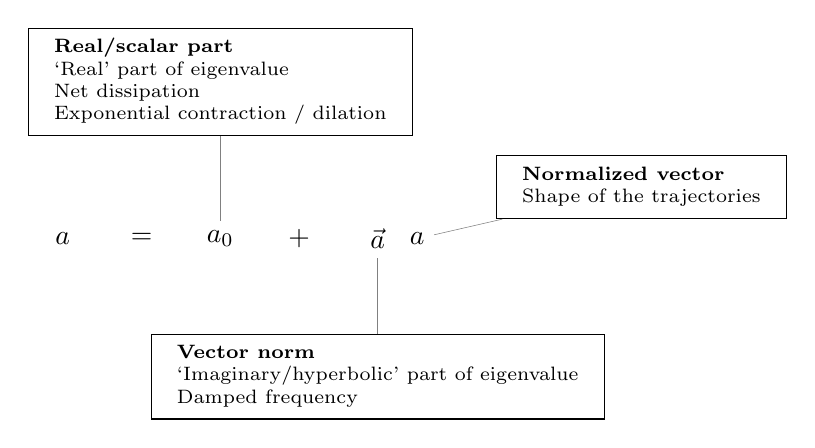
\begin{tikzpicture}
        \node (root) {$a$};
        \node[xshift=1cm] at (root) {$=$};
        \node[xshift=2cm] at (root) [pin={[below,align=left,draw,yshift=2cm] 
                                          {\scriptsize \begin{tabular}{l} \textbf{Real/scalar part} \\ `Real' part of eigenvalue \\ Net dissipation \\ Exponential contraction / dilation \end{tabular}}}] {$a_0$};
        \node[xshift=3cm] at (root) {$+$};
        \node[xshift=4cm] at (root) [pin={[above,align=left,draw,yshift=-3cm] 
                                          {\scriptsize \begin{tabular}{l} \textbf{Vector norm} \\ `Imaginary/hyperbolic' part of eigenvalue \\ Damped frequency \end{tabular}}}]{$\norm{\vec{a}}$};
        \node[xshift=4.5cm] at (root) [pin={[right,align=left,draw, xshift=1cm] 
                                          90:{\scriptsize \begin{tabular}{l} \textbf{Normalized vector} \\ Shape of the trajectories \end{tabular}}}]{$\uvec{a}$};
    \end{tikzpicture}
\end{center}

\paragraph{Normalized vector in the Lorentzian space} Since two degrees of freedom have been removed from what was originally a four-dimensional, the normalized vector part lives in a two-dimensional space. Embedded in the Lorentz space, the normalized vector parts are lie in a collection of disconnected surfaces, depending on their regime:
\begin{itemize}
    \item if $\vec{a}$ is timelike, the unit vectors live on the \emph{two-sheet unit hyperboloid}:
        $$ \qty{\vec{a} \in \real^3 \mid a_1^2 - a_2^2 - a_3^2 = 1};$$
    \item if $\vec{a}$ is lightlike, the vectors live on the \emph{light cone} (normalizing these vector is not possible):
        $$ \qty{\vec{a} \in \real^3 \mid a_1^2 - a_2^2 - a_3^2 = 0}; $$
    \item if $\vec{a}$ is spacelike, the vectors live on the \emph{one-sheet unit hyperboloid}:
        $$ \qty{\vec{a} \in \real^3 \mid a_1^2 - a_2^2 - a_3^2 = -1}. $$
\end{itemize}
These three surfaces (two-sheet hyperboloid, one-sheet hyperboloid and the light cone) are shown in \cref{fig:hyperboloids}. 

Since the regime of the mechanical system is determined by its vector norm, we can locate underdamped systems on the two-sheet hyperboloid, overdamped systems on the one-sheet hyperboloid and critically damped systems on the light cone. These surfaces are aligned along the $\quati$-axis.

\begin{figure}[ht!]
    \centering
    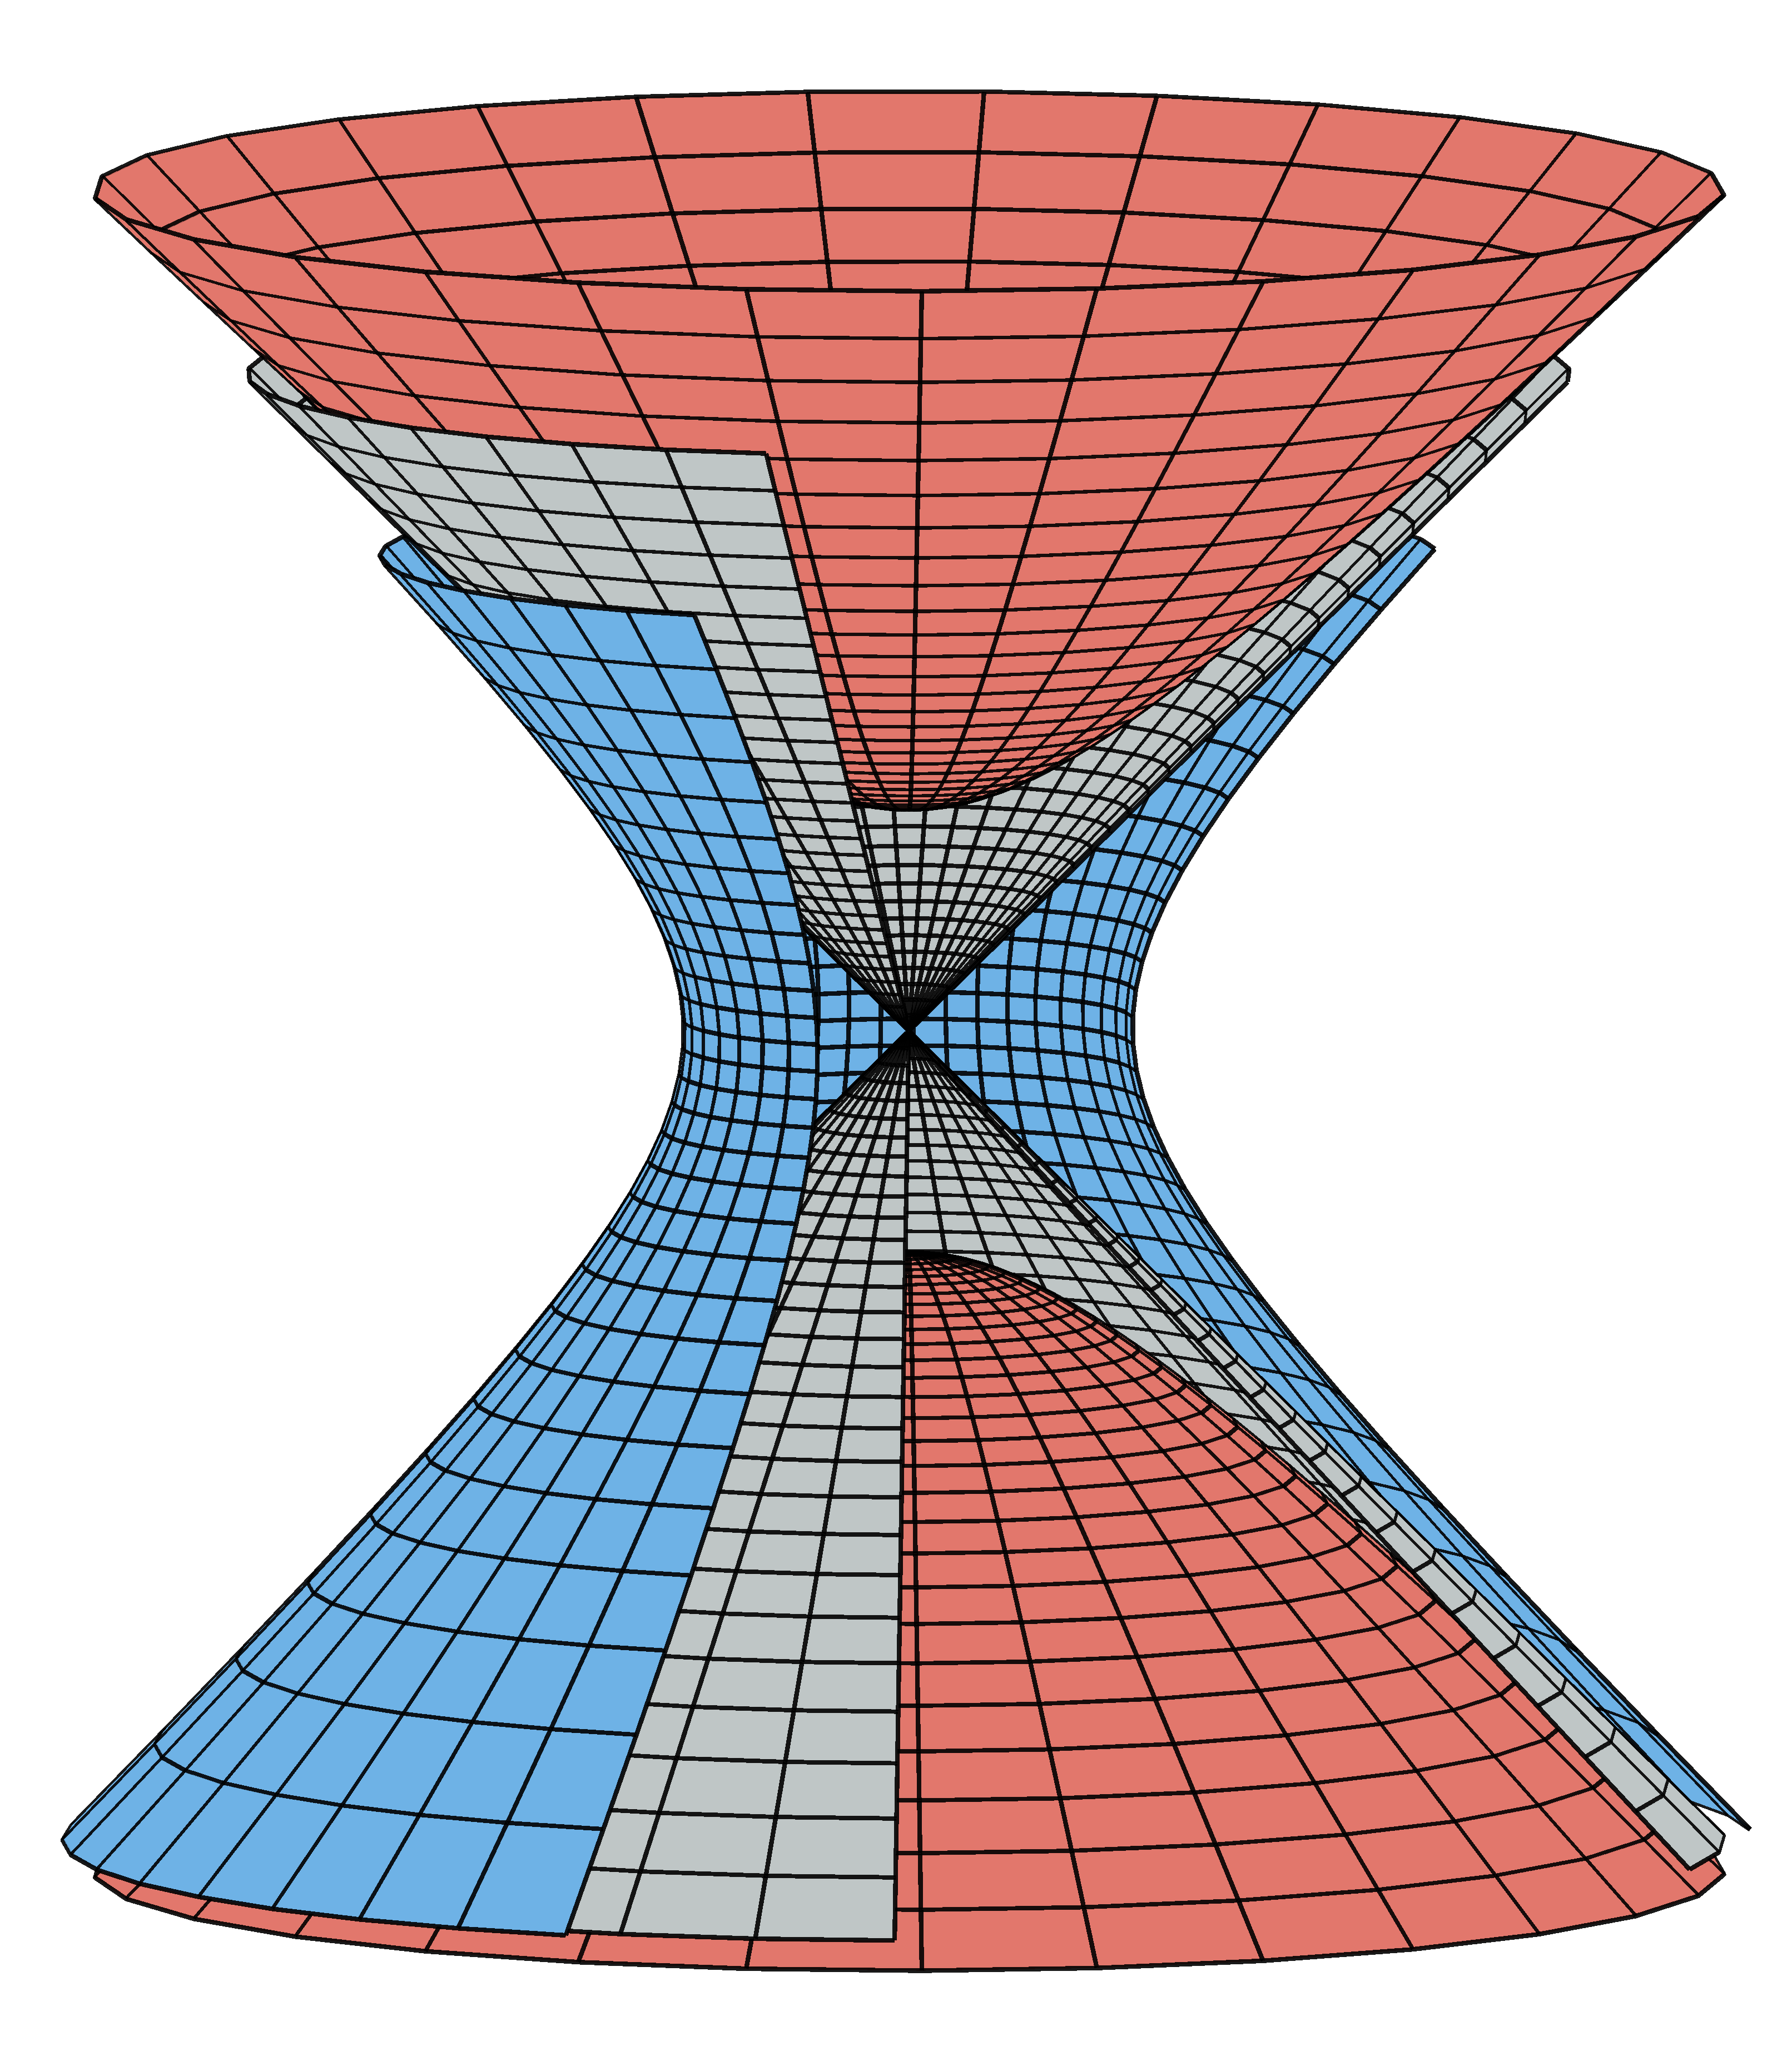
\includegraphics[]{media/other/lorentz_space.png}
    \caption{The disconnected `unit sphere' in the Lorentzian 3-space. The blue surface is the one-sheet hyperboloid, containing all the spacelike unit vectors representing overdamped mechanical systems. The gray sheet is the light cone, that contains all the lightlike `null' vectors with zero norm, representing critically damped systems. Finally, the red surfaces constitute the two-sheet hyperboloid, which is the space of all timelike unit vectors, representing underdamped (or undamped) systems.}
    \label{fig:hyperboloids}
\end{figure}

The eigenvalues represent a (composite) frequency of the system: they tell how fast the states evolve along the solution trajectories. The shape of the trajectories (given a certain regime) is encoded in the eigenvectors of the system. Hence, a certain point on each of the three surfaces shown in \cref{fig:hyperboloids} coincide with a trajectory shape, once the overall effect of damping is removed (real part), and disregarding the time parametrization along that trajectory (vector norm).

For the harmonic oscillator with two dampers, the unit vector is equal to:
$$ \uvec{a} \:= \:\qty(\frac{\tfrac{1}{m} + m\Omega_n^2}{2\Omega_d})\quati \: + \:\qty(\frac{\tfrac{1}{m} - m\Omega_n^2}{2\Omega_d})\quatj \:+ \:\qty(\frac{\gamma_p - \gamma_s}{2\Omega_d})\quatk,$$
with $\Omega_d$ being the damped frequency of the oscillator
$$ \Omega_d = \norm{\vec{a}} = \sqrt{m\Omega^2 - \tfrac{1}{4}\gamma_s - \tfrac{1}{4}\gamma_p + \tfrac{1}{2}\gamma_s \gamma_p} $$

We will now investigate the relation between the normalized vector part and the shape of the solution trajectories in each of the three cases (underdamped, critically damped and overdamped) in more detail.

\subsection{Underdamped systems}
For underdamped systems, the trajectories are spiral-shaped. Removing the real part from the split-quaternion is the same as removing the `contraction' in the spiral: as a result, the conservative version of this trajectory is an elliptic trajectory. This ellipse is subject to the same stretch and tilt of the original spiral, as illustrated by \cref{fig:underdamped}. 

The shape of the ellipse is completely determined by a measure of its eccentricity and a rotation angle (i.e. the angle between its major axis and the horizontal axis). The radius of the trajectory depends on the amount of energy present in the system and is therefore not a shape factor that is specific to the system.

\begin{figure}[ht!]
    \centering
    \begin{tikzpicture}

    \begin{axis}[%
        width=3.566in,
        height=2.566in,
        at={(1.236in,0.481in)},
        scale only axis,
        xmin=-1,
        xmax=1,
        %xlabel style={font=\color{white!15!accent3}},
        xlabel={$q$},
        ymin=-0.7,
        ymax=0.7,
        %ylabel style={font=\color{white!15!accent3, thick}},
        ylabel={$p$},
        axis background/.style={fill=white},
        %yticklabels={,,},
        %xticklabels={,,},
        %axis lines = center,
        xmajorgrids,
        xminorgrids,
        ymajorgrids,
        yminorgrids
        ]

        \addplot[-stealth, color=todoGray, point meta={sqrt((\thisrow{u})^2+(\thisrow{v})^2)}, point meta min=0, quiver={u=\thisrow{u}, v=\thisrow{v}, scale arrows = 1.45}]
         table[row sep=crcr] {%
        x	y	u	v\\
        -1	-1	-0.0980336176116068	0.071297176444805\\
        -1	-0.9	-0.0886758632032262	0.0681779249753448\\
        -1	-0.8	-0.0793181087948455	0.0650586735058845\\
        -1	-0.7	-0.0699603543864649	0.0619394220364243\\
        -1	-0.6	-0.0606025999780842	0.0588201705669641\\
        -1	-0.5	-0.0512448455697036	0.0557009190975039\\
        -1	-0.4	-0.0418870911613229	0.0525816676280437\\
        -1	-0.3	-0.0325293367529423	0.0494624161585834\\
        -1	-0.2	-0.0231715823445616	0.0463431646891232\\
        -1	-0.1	-0.013813827936181	0.043223913219663\\
        -1	0	-0.00445607352780031	0.0401046617502028\\
        -1	0.1	0.00490168088058034	0.0369854102807426\\
        -1	0.2	0.014259435288961	0.0338661588112824\\
        -1	0.3	0.0236171896973416	0.0307469073418221\\
        -1	0.4	0.0329749441057223	0.0276276558723619\\
        -1	0.5	0.0423326985141029	0.0245084044029017\\
        -1	0.6	0.0516904529224836	0.0213891529334415\\
        -1	0.7	0.0610482073308642	0.0182699014639813\\
        -1	0.8	0.0704059617392449	0.0151506499945211\\
        -1	0.9	0.0797637161476256	0.0120313985250608\\
        -1	1	0.0891214705560062	0.00891214705560062\\
        -0.9	-1	-0.0975880102588268	0.0672867102697847\\
        -0.9	-0.9	-0.0882302558504462	0.0641674588003245\\
        -0.9	-0.8	-0.0788725014420655	0.0610482073308643\\
        -0.9	-0.7	-0.0695147470336848	0.057928955861404\\
        -0.9	-0.6	-0.0601569926253042	0.0548097043919438\\
        -0.9	-0.5	-0.0507992382169235	0.0516904529224836\\
        -0.9	-0.4	-0.0414414838085429	0.0485712014530234\\
        -0.9	-0.3	-0.0320837294001622	0.0454519499835632\\
        -0.9	-0.2	-0.0227259749917816	0.0423326985141029\\
        -0.9	-0.1	-0.0133682205834009	0.0392134470446427\\
        -0.9	0	-0.00401046617502028	0.0360941955751825\\
        -0.9	0.1	0.00534728823336037	0.0329749441057223\\
        -0.9	0.2	0.014705042641741	0.0298556926362621\\
        -0.9	0.3	0.0240627970501217	0.0267364411668019\\
        -0.9	0.4	0.0334205514585023	0.0236171896973416\\
        -0.9	0.5	0.042778305866883	0.0204979382278814\\
        -0.9	0.6	0.0521360602752636	0.0173786867584212\\
        -0.9	0.7	0.0614938146836443	0.014259435288961\\
        -0.9	0.8	0.0708515690920249	0.0111401838195008\\
        -0.9	0.9	0.0802093235004056	0.00802093235004056\\
        -0.9	1	0.0895670779087862	0.00490168088058035\\
        -0.8	-1	-0.0971424029060468	0.0632762440947644\\
        -0.8	-0.9	-0.0877846484976661	0.0601569926253042\\
        -0.8	-0.8	-0.0784268940892855	0.057037741155844\\
        -0.8	-0.7	-0.0690691396809048	0.0539184896863838\\
        -0.8	-0.6	-0.0597113852725242	0.0507992382169235\\
        -0.8	-0.5	-0.0503536308641435	0.0476799867474633\\
        -0.8	-0.4	-0.0409958764557629	0.0445607352780031\\
        -0.8	-0.3	-0.0316381220473822	0.0414414838085429\\
        -0.8	-0.2	-0.0222803676390015	0.0383222323390827\\
        -0.8	-0.1	-0.0129226132306209	0.0352029808696225\\
        -0.8	0	-0.00356485882224025	0.0320837294001622\\
        -0.8	0.1	0.0057928955861404	0.028964477930702\\
        -0.8	0.2	0.0151506499945211	0.0258452264612418\\
        -0.8	0.3	0.0245084044029017	0.0227259749917816\\
        -0.8	0.4	0.0338661588112823	0.0196067235223214\\
        -0.8	0.5	0.043223913219663	0.0164874720528612\\
        -0.8	0.6	0.0525816676280437	0.0133682205834009\\
        -0.8	0.7	0.0619394220364243	0.0102489691139407\\
        -0.8	0.8	0.071297176444805	0.0071297176444805\\
        -0.8	0.9	0.0806549308531856	0.00401046617502028\\
        -0.8	1	0.0900126852615663	0.000891214705560068\\
        -0.7	-1	-0.0966967955532667	0.0592657779197441\\
        -0.7	-0.9	-0.0873390411448861	0.0561465264502839\\
        -0.7	-0.8	-0.0779812867365054	0.0530272749808237\\
        -0.7	-0.7	-0.0686235323281248	0.0499080235113635\\
        -0.7	-0.6	-0.0592657779197441	0.0467887720419033\\
        -0.7	-0.5	-0.0499080235113635	0.043669520572443\\
        -0.7	-0.4	-0.0405502691029828	0.0405502691029828\\
        -0.7	-0.3	-0.0311925146946022	0.0374310176335226\\
        -0.7	-0.2	-0.0218347602862215	0.0343117661640624\\
        -0.7	-0.1	-0.0124770058778409	0.0311925146946022\\
        -0.7	0	-0.00311925146946022	0.028073263225142\\
        -0.7	0.1	0.00623850293892043	0.0249540117556817\\
        -0.7	0.2	0.0155962573473011	0.0218347602862215\\
        -0.7	0.3	0.0249540117556817	0.0187155088167613\\
        -0.7	0.4	0.0343117661640624	0.0155962573473011\\
        -0.7	0.5	0.043669520572443	0.0124770058778409\\
        -0.7	0.6	0.0530272749808237	0.00935775440838065\\
        -0.7	0.7	0.0623850293892043	0.00623850293892044\\
        -0.7	0.8	0.071742783797585	0.00311925146946022\\
        -0.7	0.9	0.0811005382059656	0\\
        -0.7	1	0.0904582926143463	-0.00311925146946022\\
        -0.6	-1	-0.0962511882004867	0.0552553117447238\\
        -0.6	-0.9	-0.0868934337921061	0.0521360602752636\\
        -0.6	-0.8	-0.0775356793837254	0.0490168088058034\\
        -0.6	-0.7	-0.0681779249753448	0.0458975573363432\\
        -0.6	-0.6	-0.0588201705669641	0.042778305866883\\
        -0.6	-0.5	-0.0494624161585834	0.0396590543974228\\
        -0.6	-0.4	-0.0401046617502028	0.0365398029279625\\
        -0.6	-0.3	-0.0307469073418221	0.0334205514585023\\
        -0.6	-0.2	-0.0213891529334415	0.0303012999890421\\
        -0.6	-0.1	-0.0120313985250608	0.0271820485195819\\
        -0.6	0	-0.00267364411668019	0.0240627970501217\\
        -0.6	0.1	0.00668411029170046	0.0209435455806615\\
        -0.6	0.2	0.0160418647000811	0.0178242941112012\\
        -0.6	0.3	0.0253996191084618	0.014705042641741\\
        -0.6	0.4	0.0347573735168424	0.0115857911722808\\
        -0.6	0.5	0.0441151279252231	0.00846653970282059\\
        -0.6	0.6	0.0534728823336037	0.00534728823336037\\
        -0.6	0.7	0.0628306367419844	0.00222803676390016\\
        -0.6	0.8	0.072188391150365	-0.000891214705560058\\
        -0.6	0.9	0.0815461455587457	-0.00401046617502028\\
        -0.6	1	0.0909038999671263	-0.00712971764448049\\
        -0.5	-1	-0.0958055808477067	0.0512448455697036\\
        -0.5	-0.9	-0.086447826439326	0.0481255941002434\\
        -0.5	-0.8	-0.0770900720309454	0.0450063426307831\\
        -0.5	-0.7	-0.0677323176225647	0.0418870911613229\\
        -0.5	-0.6	-0.0583745632141841	0.0387678396918627\\
        -0.5	-0.5	-0.0490168088058034	0.0356485882224025\\
        -0.5	-0.4	-0.0396590543974228	0.0325293367529423\\
        -0.5	-0.3	-0.0303012999890421	0.029410085283482\\
        -0.5	-0.2	-0.0209435455806615	0.0262908338140218\\
        -0.5	-0.1	-0.0115857911722808	0.0231715823445616\\
        -0.5	0	-0.00222803676390016	0.0200523308751014\\
        -0.5	0.1	0.00712971764448049	0.0169330794056412\\
        -0.5	0.2	0.0164874720528611	0.013813827936181\\
        -0.5	0.3	0.0258452264612418	0.0106945764667207\\
        -0.5	0.4	0.0352029808696224	0.00757532499726053\\
        -0.5	0.5	0.0445607352780031	0.00445607352780031\\
        -0.5	0.6	0.0539184896863838	0.00133682205834009\\
        -0.5	0.7	0.0632762440947644	-0.00178242941112012\\
        -0.5	0.8	0.0726339985031451	-0.00490168088058034\\
        -0.5	0.9	0.0819917529115257	-0.00802093235004056\\
        -0.5	1	0.0913495073199064	-0.0111401838195008\\
        -0.4	-1	-0.0953599734949266	0.0472343793946833\\
        -0.4	-0.9	-0.086002219086546	0.0441151279252231\\
        -0.4	-0.8	-0.0766444646781654	0.0409958764557629\\
        -0.4	-0.7	-0.0672867102697847	0.0378766249863026\\
        -0.4	-0.6	-0.057928955861404	0.0347573735168424\\
        -0.4	-0.5	-0.0485712014530234	0.0316381220473822\\
        -0.4	-0.4	-0.0392134470446427	0.028518870577922\\
        -0.4	-0.3	-0.0298556926362621	0.0253996191084618\\
        -0.4	-0.2	-0.0204979382278814	0.0222803676390015\\
        -0.4	-0.1	-0.0111401838195008	0.0191611161695413\\
        -0.4	0	-0.00178242941112012	0.0160418647000811\\
        -0.4	0.1	0.00757532499726053	0.0129226132306209\\
        -0.4	0.2	0.0169330794056412	0.00980336176116068\\
        -0.4	0.3	0.0262908338140218	0.00668411029170047\\
        -0.4	0.4	0.0356485882224025	0.00356485882224025\\
        -0.4	0.5	0.0450063426307831	0.000445607352780029\\
        -0.4	0.6	0.0543640970391638	-0.00267364411668019\\
        -0.4	0.7	0.0637218514475444	-0.0057928955861404\\
        -0.4	0.8	0.0730796058559251	-0.00891214705560062\\
        -0.4	0.9	0.0824373602643057	-0.0120313985250608\\
        -0.4	1	0.0917951146726864	-0.0151506499945211\\
        -0.3	-1	-0.0949143661421466	0.043223913219663\\
        -0.3	-0.9	-0.085556611733766	0.0401046617502028\\
        -0.3	-0.8	-0.0761988573253853	0.0369854102807426\\
        -0.3	-0.7	-0.0668411029170047	0.0338661588112824\\
        -0.3	-0.6	-0.057483348508624	0.0307469073418221\\
        -0.3	-0.5	-0.0481255941002434	0.0276276558723619\\
        -0.3	-0.4	-0.0387678396918627	0.0245084044029017\\
        -0.3	-0.3	-0.029410085283482	0.0213891529334415\\
        -0.3	-0.2	-0.0200523308751014	0.0182699014639813\\
        -0.3	-0.1	-0.0106945764667207	0.0151506499945211\\
        -0.3	0	-0.00133682205834009	0.0120313985250608\\
        -0.3	0.1	0.00802093235004056	0.00891214705560062\\
        -0.3	0.2	0.0173786867584212	0.0057928955861404\\
        -0.3	0.3	0.0267364411668019	0.00267364411668019\\
        -0.3	0.4	0.0360941955751825	-0.000445607352780029\\
        -0.3	0.5	0.0454519499835632	-0.00356485882224025\\
        -0.3	0.6	0.0548097043919438	-0.00668411029170047\\
        -0.3	0.7	0.0641674588003245	-0.00980336176116068\\
        -0.3	0.8	0.0735252132087051	-0.0129226132306209\\
        -0.3	0.9	0.0828829676170858	-0.0160418647000811\\
        -0.3	1	0.0922407220254664	-0.0191611161695413\\
        -0.2	-1	-0.0944687587893666	0.0392134470446427\\
        -0.2	-0.9	-0.0851110043809859	0.0360941955751825\\
        -0.2	-0.8	-0.0757532499726053	0.0329749441057223\\
        -0.2	-0.7	-0.0663954955642246	0.0298556926362621\\
        -0.2	-0.6	-0.057037741155844	0.0267364411668019\\
        -0.2	-0.5	-0.0476799867474633	0.0236171896973416\\
        -0.2	-0.4	-0.0383222323390827	0.0204979382278814\\
        -0.2	-0.3	-0.028964477930702	0.0173786867584212\\
        -0.2	-0.2	-0.0196067235223214	0.014259435288961\\
        -0.2	-0.1	-0.0102489691139407	0.0111401838195008\\
        -0.2	0	-0.000891214705560062	0.00802093235004056\\
        -0.2	0.1	0.00846653970282059	0.00490168088058034\\
        -0.2	0.2	0.0178242941112012	0.00178242941112012\\
        -0.2	0.3	0.0271820485195819	-0.00133682205834009\\
        -0.2	0.4	0.0365398029279625	-0.00445607352780031\\
        -0.2	0.5	0.0458975573363432	-0.00757532499726053\\
        -0.2	0.6	0.0552553117447238	-0.0106945764667207\\
        -0.2	0.7	0.0646130661531045	-0.013813827936181\\
        -0.2	0.8	0.0739708205614852	-0.0169330794056412\\
        -0.2	0.9	0.0833285749698658	-0.0200523308751014\\
        -0.2	1	0.0926863293782465	-0.0231715823445616\\
        -0.1	-1	-0.0940231514365865	0.0352029808696224\\
        -0.1	-0.9	-0.0846653970282059	0.0320837294001622\\
        -0.1	-0.8	-0.0753076426198253	0.028964477930702\\
        -0.1	-0.7	-0.0659498882114446	0.0258452264612418\\
        -0.1	-0.6	-0.0565921338030639	0.0227259749917816\\
        -0.1	-0.5	-0.0472343793946833	0.0196067235223214\\
        -0.1	-0.4	-0.0378766249863026	0.0164874720528611\\
        -0.1	-0.3	-0.028518870577922	0.0133682205834009\\
        -0.1	-0.2	-0.0191611161695413	0.0102489691139407\\
        -0.1	-0.1	-0.00980336176116068	0.0071297176444805\\
        -0.1	0	-0.000445607352780031	0.00401046617502028\\
        -0.1	0.1	0.00891214705560062	0.000891214705560062\\
        -0.1	0.2	0.0182699014639813	-0.00222803676390015\\
        -0.1	0.3	0.0276276558723619	-0.00534728823336037\\
        -0.1	0.4	0.0369854102807426	-0.00846653970282059\\
        -0.1	0.5	0.0463431646891232	-0.0115857911722808\\
        -0.1	0.6	0.0557009190975039	-0.014705042641741\\
        -0.1	0.7	0.0650586735058845	-0.0178242941112012\\
        -0.1	0.8	0.0744164279142652	-0.0209435455806615\\
        -0.1	0.9	0.0837741823226458	-0.0240627970501217\\
        -0.1	1	0.0931319367310265	-0.0271820485195819\\
        0	-1	-0.0935775440838065	0.0311925146946022\\
        0	-0.9	-0.0842197896754259	0.028073263225142\\
        0	-0.8	-0.0748620352670452	0.0249540117556817\\
        0	-0.7	-0.0655042808586646	0.0218347602862215\\
        0	-0.6	-0.0561465264502839	0.0187155088167613\\
        0	-0.5	-0.0467887720419033	0.0155962573473011\\
        0	-0.4	-0.0374310176335226	0.0124770058778409\\
        0	-0.3	-0.028073263225142	0.00935775440838065\\
        0	-0.2	-0.0187155088167613	0.00623850293892043\\
        0	-0.1	-0.00935775440838065	0.00311925146946022\\
        0	0	0	-0\\
        0	0.1	0.00935775440838065	-0.00311925146946022\\
        0	0.2	0.0187155088167613	-0.00623850293892043\\
        0	0.3	0.028073263225142	-0.00935775440838065\\
        0	0.4	0.0374310176335226	-0.0124770058778409\\
        0	0.5	0.0467887720419033	-0.0155962573473011\\
        0	0.6	0.0561465264502839	-0.0187155088167613\\
        0	0.7	0.0655042808586646	-0.0218347602862215\\
        0	0.8	0.0748620352670452	-0.0249540117556817\\
        0	0.9	0.0842197896754259	-0.028073263225142\\
        0	1	0.0935775440838065	-0.0311925146946022\\
        0.1	-1	-0.0931319367310265	0.0271820485195819\\
        0.1	-0.9	-0.0837741823226458	0.0240627970501217\\
        0.1	-0.8	-0.0744164279142652	0.0209435455806615\\
        0.1	-0.7	-0.0650586735058845	0.0178242941112012\\
        0.1	-0.6	-0.0557009190975039	0.014705042641741\\
        0.1	-0.5	-0.0463431646891232	0.0115857911722808\\
        0.1	-0.4	-0.0369854102807426	0.00846653970282059\\
        0.1	-0.3	-0.0276276558723619	0.00534728823336037\\
        0.1	-0.2	-0.0182699014639813	0.00222803676390015\\
        0.1	-0.1	-0.00891214705560062	-0.000891214705560062\\
        0.1	0	0.000445607352780031	-0.00401046617502028\\
        0.1	0.1	0.00980336176116068	-0.0071297176444805\\
        0.1	0.2	0.0191611161695413	-0.0102489691139407\\
        0.1	0.3	0.028518870577922	-0.0133682205834009\\
        0.1	0.4	0.0378766249863026	-0.0164874720528611\\
        0.1	0.5	0.0472343793946833	-0.0196067235223214\\
        0.1	0.6	0.0565921338030639	-0.0227259749917816\\
        0.1	0.7	0.0659498882114446	-0.0258452264612418\\
        0.1	0.8	0.0753076426198253	-0.028964477930702\\
        0.1	0.9	0.0846653970282059	-0.0320837294001622\\
        0.1	1	0.0940231514365865	-0.0352029808696224\\
        0.2	-1	-0.0926863293782465	0.0231715823445616\\
        0.2	-0.9	-0.0833285749698658	0.0200523308751014\\
        0.2	-0.8	-0.0739708205614852	0.0169330794056412\\
        0.2	-0.7	-0.0646130661531045	0.013813827936181\\
        0.2	-0.6	-0.0552553117447238	0.0106945764667207\\
        0.2	-0.5	-0.0458975573363432	0.00757532499726053\\
        0.2	-0.4	-0.0365398029279625	0.00445607352780031\\
        0.2	-0.3	-0.0271820485195819	0.00133682205834009\\
        0.2	-0.2	-0.0178242941112012	-0.00178242941112012\\
        0.2	-0.1	-0.00846653970282059	-0.00490168088058034\\
        0.2	0	0.000891214705560062	-0.00802093235004056\\
        0.2	0.1	0.0102489691139407	-0.0111401838195008\\
        0.2	0.2	0.0196067235223214	-0.014259435288961\\
        0.2	0.3	0.028964477930702	-0.0173786867584212\\
        0.2	0.4	0.0383222323390827	-0.0204979382278814\\
        0.2	0.5	0.0476799867474633	-0.0236171896973416\\
        0.2	0.6	0.057037741155844	-0.0267364411668019\\
        0.2	0.7	0.0663954955642246	-0.0298556926362621\\
        0.2	0.8	0.0757532499726053	-0.0329749441057223\\
        0.2	0.9	0.0851110043809859	-0.0360941955751825\\
        0.2	1	0.0944687587893666	-0.0392134470446427\\
        0.3	-1	-0.0922407220254664	0.0191611161695413\\
        0.3	-0.9	-0.0828829676170858	0.0160418647000811\\
        0.3	-0.8	-0.0735252132087051	0.0129226132306209\\
        0.3	-0.7	-0.0641674588003245	0.00980336176116068\\
        0.3	-0.6	-0.0548097043919438	0.00668411029170047\\
        0.3	-0.5	-0.0454519499835632	0.00356485882224025\\
        0.3	-0.4	-0.0360941955751825	0.000445607352780029\\
        0.3	-0.3	-0.0267364411668019	-0.00267364411668019\\
        0.3	-0.2	-0.0173786867584212	-0.0057928955861404\\
        0.3	-0.1	-0.00802093235004056	-0.00891214705560062\\
        0.3	0	0.00133682205834009	-0.0120313985250608\\
        0.3	0.1	0.0106945764667207	-0.0151506499945211\\
        0.3	0.2	0.0200523308751014	-0.0182699014639813\\
        0.3	0.3	0.029410085283482	-0.0213891529334415\\
        0.3	0.4	0.0387678396918627	-0.0245084044029017\\
        0.3	0.5	0.0481255941002434	-0.0276276558723619\\
        0.3	0.6	0.057483348508624	-0.0307469073418221\\
        0.3	0.7	0.0668411029170047	-0.0338661588112824\\
        0.3	0.8	0.0761988573253853	-0.0369854102807426\\
        0.3	0.9	0.085556611733766	-0.0401046617502028\\
        0.3	1	0.0949143661421466	-0.043223913219663\\
        0.4	-1	-0.0917951146726864	0.0151506499945211\\
        0.4	-0.9	-0.0824373602643057	0.0120313985250608\\
        0.4	-0.8	-0.0730796058559251	0.00891214705560062\\
        0.4	-0.7	-0.0637218514475444	0.0057928955861404\\
        0.4	-0.6	-0.0543640970391638	0.00267364411668019\\
        0.4	-0.5	-0.0450063426307831	-0.000445607352780029\\
        0.4	-0.4	-0.0356485882224025	-0.00356485882224025\\
        0.4	-0.3	-0.0262908338140218	-0.00668411029170047\\
        0.4	-0.2	-0.0169330794056412	-0.00980336176116068\\
        0.4	-0.1	-0.00757532499726053	-0.0129226132306209\\
        0.4	0	0.00178242941112012	-0.0160418647000811\\
        0.4	0.1	0.0111401838195008	-0.0191611161695413\\
        0.4	0.2	0.0204979382278814	-0.0222803676390015\\
        0.4	0.3	0.0298556926362621	-0.0253996191084618\\
        0.4	0.4	0.0392134470446427	-0.028518870577922\\
        0.4	0.5	0.0485712014530234	-0.0316381220473822\\
        0.4	0.6	0.057928955861404	-0.0347573735168424\\
        0.4	0.7	0.0672867102697847	-0.0378766249863026\\
        0.4	0.8	0.0766444646781654	-0.0409958764557629\\
        0.4	0.9	0.086002219086546	-0.0441151279252231\\
        0.4	1	0.0953599734949266	-0.0472343793946833\\
        0.5	-1	-0.0913495073199064	0.0111401838195008\\
        0.5	-0.9	-0.0819917529115257	0.00802093235004056\\
        0.5	-0.8	-0.0726339985031451	0.00490168088058034\\
        0.5	-0.7	-0.0632762440947644	0.00178242941112012\\
        0.5	-0.6	-0.0539184896863838	-0.00133682205834009\\
        0.5	-0.5	-0.0445607352780031	-0.00445607352780031\\
        0.5	-0.4	-0.0352029808696224	-0.00757532499726053\\
        0.5	-0.3	-0.0258452264612418	-0.0106945764667207\\
        0.5	-0.2	-0.0164874720528611	-0.013813827936181\\
        0.5	-0.1	-0.00712971764448049	-0.0169330794056412\\
        0.5	0	0.00222803676390016	-0.0200523308751014\\
        0.5	0.1	0.0115857911722808	-0.0231715823445616\\
        0.5	0.2	0.0209435455806615	-0.0262908338140218\\
        0.5	0.3	0.0303012999890421	-0.029410085283482\\
        0.5	0.4	0.0396590543974228	-0.0325293367529423\\
        0.5	0.5	0.0490168088058034	-0.0356485882224025\\
        0.5	0.6	0.0583745632141841	-0.0387678396918627\\
        0.5	0.7	0.0677323176225647	-0.0418870911613229\\
        0.5	0.8	0.0770900720309454	-0.0450063426307831\\
        0.5	0.9	0.086447826439326	-0.0481255941002434\\
        0.5	1	0.0958055808477067	-0.0512448455697036\\
        0.6	-1	-0.0909038999671263	0.00712971764448049\\
        0.6	-0.9	-0.0815461455587457	0.00401046617502028\\
        0.6	-0.8	-0.072188391150365	0.000891214705560058\\
        0.6	-0.7	-0.0628306367419844	-0.00222803676390016\\
        0.6	-0.6	-0.0534728823336037	-0.00534728823336037\\
        0.6	-0.5	-0.0441151279252231	-0.00846653970282059\\
        0.6	-0.4	-0.0347573735168424	-0.0115857911722808\\
        0.6	-0.3	-0.0253996191084618	-0.014705042641741\\
        0.6	-0.2	-0.0160418647000811	-0.0178242941112012\\
        0.6	-0.1	-0.00668411029170046	-0.0209435455806615\\
        0.6	0	0.00267364411668019	-0.0240627970501217\\
        0.6	0.1	0.0120313985250608	-0.0271820485195819\\
        0.6	0.2	0.0213891529334415	-0.0303012999890421\\
        0.6	0.3	0.0307469073418221	-0.0334205514585023\\
        0.6	0.4	0.0401046617502028	-0.0365398029279625\\
        0.6	0.5	0.0494624161585834	-0.0396590543974228\\
        0.6	0.6	0.0588201705669641	-0.042778305866883\\
        0.6	0.7	0.0681779249753448	-0.0458975573363432\\
        0.6	0.8	0.0775356793837254	-0.0490168088058034\\
        0.6	0.9	0.0868934337921061	-0.0521360602752636\\
        0.6	1	0.0962511882004867	-0.0552553117447238\\
        0.7	-1	-0.0904582926143463	0.00311925146946022\\
        0.7	-0.9	-0.0811005382059656	0\\
        0.7	-0.8	-0.071742783797585	-0.00311925146946022\\
        0.7	-0.7	-0.0623850293892043	-0.00623850293892044\\
        0.7	-0.6	-0.0530272749808237	-0.00935775440838065\\
        0.7	-0.5	-0.043669520572443	-0.0124770058778409\\
        0.7	-0.4	-0.0343117661640624	-0.0155962573473011\\
        0.7	-0.3	-0.0249540117556817	-0.0187155088167613\\
        0.7	-0.2	-0.0155962573473011	-0.0218347602862215\\
        0.7	-0.1	-0.00623850293892043	-0.0249540117556817\\
        0.7	0	0.00311925146946022	-0.028073263225142\\
        0.7	0.1	0.0124770058778409	-0.0311925146946022\\
        0.7	0.2	0.0218347602862215	-0.0343117661640624\\
        0.7	0.3	0.0311925146946022	-0.0374310176335226\\
        0.7	0.4	0.0405502691029828	-0.0405502691029828\\
        0.7	0.5	0.0499080235113635	-0.043669520572443\\
        0.7	0.6	0.0592657779197441	-0.0467887720419033\\
        0.7	0.7	0.0686235323281248	-0.0499080235113635\\
        0.7	0.8	0.0779812867365054	-0.0530272749808237\\
        0.7	0.9	0.0873390411448861	-0.0561465264502839\\
        0.7	1	0.0966967955532667	-0.0592657779197441\\
        0.8	-1	-0.0900126852615663	-0.000891214705560068\\
        0.8	-0.9	-0.0806549308531856	-0.00401046617502028\\
        0.8	-0.8	-0.071297176444805	-0.0071297176444805\\
        0.8	-0.7	-0.0619394220364243	-0.0102489691139407\\
        0.8	-0.6	-0.0525816676280437	-0.0133682205834009\\
        0.8	-0.5	-0.043223913219663	-0.0164874720528612\\
        0.8	-0.4	-0.0338661588112823	-0.0196067235223214\\
        0.8	-0.3	-0.0245084044029017	-0.0227259749917816\\
        0.8	-0.2	-0.0151506499945211	-0.0258452264612418\\
        0.8	-0.1	-0.0057928955861404	-0.028964477930702\\
        0.8	0	0.00356485882224025	-0.0320837294001622\\
        0.8	0.1	0.0129226132306209	-0.0352029808696225\\
        0.8	0.2	0.0222803676390015	-0.0383222323390827\\
        0.8	0.3	0.0316381220473822	-0.0414414838085429\\
        0.8	0.4	0.0409958764557629	-0.0445607352780031\\
        0.8	0.5	0.0503536308641435	-0.0476799867474633\\
        0.8	0.6	0.0597113852725242	-0.0507992382169235\\
        0.8	0.7	0.0690691396809048	-0.0539184896863838\\
        0.8	0.8	0.0784268940892855	-0.057037741155844\\
        0.8	0.9	0.0877846484976661	-0.0601569926253042\\
        0.8	1	0.0971424029060468	-0.0632762440947644\\
        0.9	-1	-0.0895670779087862	-0.00490168088058035\\
        0.9	-0.9	-0.0802093235004056	-0.00802093235004056\\
        0.9	-0.8	-0.0708515690920249	-0.0111401838195008\\
        0.9	-0.7	-0.0614938146836443	-0.014259435288961\\
        0.9	-0.6	-0.0521360602752636	-0.0173786867584212\\
        0.9	-0.5	-0.042778305866883	-0.0204979382278814\\
        0.9	-0.4	-0.0334205514585023	-0.0236171896973416\\
        0.9	-0.3	-0.0240627970501217	-0.0267364411668019\\
        0.9	-0.2	-0.014705042641741	-0.0298556926362621\\
        0.9	-0.1	-0.00534728823336037	-0.0329749441057223\\
        0.9	0	0.00401046617502028	-0.0360941955751825\\
        0.9	0.1	0.0133682205834009	-0.0392134470446427\\
        0.9	0.2	0.0227259749917816	-0.0423326985141029\\
        0.9	0.3	0.0320837294001622	-0.0454519499835632\\
        0.9	0.4	0.0414414838085429	-0.0485712014530234\\
        0.9	0.5	0.0507992382169235	-0.0516904529224836\\
        0.9	0.6	0.0601569926253042	-0.0548097043919438\\
        0.9	0.7	0.0695147470336848	-0.057928955861404\\
        0.9	0.8	0.0788725014420655	-0.0610482073308643\\
        0.9	0.9	0.0882302558504462	-0.0641674588003245\\
        0.9	1	0.0975880102588268	-0.0672867102697847\\
        1	-1	-0.0891214705560062	-0.00891214705560062\\
        1	-0.9	-0.0797637161476256	-0.0120313985250608\\
        1	-0.8	-0.0704059617392449	-0.0151506499945211\\
        1	-0.7	-0.0610482073308642	-0.0182699014639813\\
        1	-0.6	-0.0516904529224836	-0.0213891529334415\\
        1	-0.5	-0.0423326985141029	-0.0245084044029017\\
        1	-0.4	-0.0329749441057223	-0.0276276558723619\\
        1	-0.3	-0.0236171896973416	-0.0307469073418221\\
        1	-0.2	-0.014259435288961	-0.0338661588112824\\
        1	-0.1	-0.00490168088058034	-0.0369854102807426\\
        1	0	0.00445607352780031	-0.0401046617502028\\
        1	0.1	0.013813827936181	-0.043223913219663\\
        1	0.2	0.0231715823445616	-0.0463431646891232\\
        1	0.3	0.0325293367529423	-0.0494624161585834\\
        1	0.4	0.0418870911613229	-0.0525816676280437\\
        1	0.5	0.0512448455697036	-0.0557009190975039\\
        1	0.6	0.0606025999780842	-0.0588201705669641\\
        1	0.7	0.0699603543864649	-0.0619394220364243\\
        1	0.8	0.0793181087948455	-0.0650586735058845\\
        1	0.9	0.0886758632032262	-0.0681779249753448\\
        1	1	0.0980336176116068	-0.071297176444805\\
        };
        \addplot [color=accent1,  line width=1.2pt, forget plot]
          table[row sep=crcr]{%
        0.2	0\\
        0.20078267718294	-0.00179994810044893\\
        0.201530619463493	-0.00359958481436568\\
        0.20224369744951	-0.00539859880908716\\
        0.202921787780278	-0.00719667885967914\\
        0.203564773147861	-0.00899351390277742\\
        0.204172542317393	-0.0107887930904009\\
        0.204744990146326	-0.0125822058437278\\
        0.205282017602611	-0.0143734419068246\\
        0.205783531781838	-0.0161621914003199\\
        0.206249445923306	-0.0179481448750126\\
        0.206679679425029	-0.0197309933654058\\
        0.207074157857685	-0.0215104284431572\\
        0.207432812977489	-0.0232861422704365\\
        0.207755582737999	-0.0250578276531802\\
        0.208042411300853	-0.0268251780942358\\
        0.208293249045423	-0.028587887846385\\
        0.208508052577407	-0.030345651965237\\
        0.208686784736328	-0.0320981663619831\\
        0.208829414601969	-0.0338451278560036\\
        0.208935917499719	-0.0355862342273171\\
        0.209006275004841	-0.0373211842688638\\
        0.209040474945664	-0.0390496778386136\\
        0.209038511405683	-0.0407714159114899\\
        0.209000384724585	-0.0424861006311003\\
        0.208926101498191	-0.0441934353612647\\
        0.208815674577315	-0.0458931247373331\\
        0.208669123065536	-0.0475848747172826\\
        0.208486472315903	-0.0492683926325859\\
        0.208267753926539	-0.0509433872388425\\
        0.208013005735179	-0.0526095687661632\\
        0.207722271812626	-0.0542666489692992\\
        0.207395602455123	-0.0559143411775083\\
        0.207033054175655	-0.0575523603441479\\
        0.206634689694169	-0.0591804230959875\\
        0.206200577926726	-0.0607982477822316\\
        0.205730793973581	-0.0624055545232443\\
        0.205225419106186	-0.0640020652589683\\
        0.204684540753131	-0.0655875037970281\\
        0.204108252485023	-0.0671615958605107\\
        0.203496653998296	-0.0687240691354152\\
        0.202849851097961	-0.0702746533177617\\
        0.202167955679308	-0.0718130801603541\\
        0.201451085708543	-0.0733390835191855\\
        0.200699365202384	-0.0748523993994809\\
        0.199912924206603	-0.0763527660013672\\
        0.19909189877353	-0.0778399237651643\\
        0.198236430938519	-0.0793136154162882\\
        0.19734666869537	-0.0807735860097587\\
        0.196422765970734	-0.0822195829743043\\
        0.195464882597476	-0.0836513561560568\\
        0.194473184287033	-0.0850686578618265\\
        0.193447842600736	-0.0864712429019532\\
        0.192389034920143	-0.0878588686327231\\
        0.191296944416339	-0.0892312949983456\\
        0.19017176001826	-0.0905882845724824\\
        0.189013676379998	-0.0919296025993216\\
        0.187822893847136	-0.0932550170341899\\
        0.186599618422082	-0.0945642985836957\\
        0.185344061728433	-0.0958572207453964\\
        0.184056440974366	-0.0971335598469827\\
        0.18273697891506	-0.0983930950849732\\
        0.18138590381416	-0.0996356085629132\\
        0.180003449404289	-0.10086088532907\\
        0.178589854846612	-0.102068713413619\\
        0.177145364689462	-0.103258883865313\\
        0.175670228826034	-0.104431190787634\\
        0.174164702451153	-0.105585431374407\\
        0.172629046017126	-0.10672140594489\\
        0.171063525188687	-0.107838917978314\\
        0.169468410797034	-0.108937774147886\\
        0.16784397879298	-0.110017784354229\\
        0.166190510199209	-0.111078761758271\\
        0.164508291061664	-0.112120522813566\\
        0.16279761240006	-0.113142887298051\\
        0.161058770157539	-0.11414567834522\\
        0.159292065149473	-0.115128722474722\\
        0.157497803011422	-0.116091849622375\\
        0.15567629414626	-0.117034893169584\\
        0.153827853670478	-0.117957689972168\\
        0.151952801359668	-0.118860080388582\\
        0.150051461593204	-0.119741908307533\\
        0.148124163298123	-0.120603021174992\\
        0.146171239892223	-0.12144327002058\\
        0.144193029226383	-0.122262509483342\\
        0.142189873526114	-0.123060597836895\\
        0.140162119332357	-0.123837397013943\\
        0.138110117441529	-0.124592772630168\\
        0.13603422284484	-0.12532659400747\\
        0.133934794666877	-0.126038734196582\\
        0.13181219610348	-0.126729069999027\\
        0.129666794358905	-0.127397481988433\\
        0.127498960582305	-0.128043854531194\\
        0.125309069803514	-0.128668075806471\\
        0.123097500868178	-0.12927003782554\\
        0.120864636372204	-0.129849636450474\\
        0.118610862595583	-0.130406771412156\\
        0.116336569435557	-0.130941346327627\\
        0.114042150339169	-0.13145326871676\\
        0.111728002235202	-0.131942450018259\\
        0.109394525465506	-0.132408805604978\\
        0.107042123715742	-0.132852254798564\\
        0.104671203945545	-0.133272720883413\\
        0.102282176318123	-0.13367013111994\\
        0.0998754541292964	-0.134044416757166\\
        0.0974514537360019	-0.134395513044609\\
        0.0950105944842618	-0.134723359243487\\
        0.0925532986366388	-0.135027898637226\\
        0.090079991299186	-0.135309078541268\\
        0.0875911003479041	-0.135566850312194\\
        0.0850870563547203	-0.135801169356128\\
        0.0825682925130001	-0.136011995136462\\
        0.0800352445626062	-0.13619929118086\\
        0.0774883507145164	-0.136363025087574\\
        0.0749280515750143	-0.136503168531047\\
        0.0723547900694654	-0.136619697266812\\
        0.0697690113656923	-0.136712591135689\\
        0.0671711627969617	-0.13678183406727\\
        0.0645616937845967	-0.136827414082701\\
        0.0619410557602283	-0.136849323296752\\
        0.0593097020876986	-0.136847557919185\\
        0.0566680879846303	-0.136822118255405\\
        0.0540166704436747	-0.136773008706411\\
        0.0513559081534537	-0.136700237768032\\
        0.0486862614192073	-0.136603818029459\\
        0.0460081920831623	-0.136483766171066\\
        0.0433221634446345	-0.136340102961525\\
        0.0406286401798793	-0.136172853254213\\
        0.0379280882617035	-0.135982045982914\\
        0.0352209748788538	-0.135767714156807\\
        0.0325077683551935	-0.135529894854766\\
        0.0297889380686844	-0.135268629218935\\
        0.0270649543701851	-0.134983962447619\\
        0.0243362885020816	-0.134675943787459\\
        0.0216034125167637	-0.134344626524915\\
        0.0188667991949607	-0.133990067977047\\
        0.0161269219639521	-0.133612329481599\\
        0.0133842548156654	-0.133211476386389\\
        0.0106392722246768	-0.132787578038003\\
        0.00789244906612849	-0.132340707769798\\
        0.00514426053357601	-0.131870942889215\\
        0.00239518205678137	-0.131378364664408\\
        -0.000354310780535346	-0.130863058310181\\
        -0.00310374232297071	-0.130325112973247\\
        -0.00585263692572514	-0.129764621716809\\
        -0.0086005190368883	-0.129181681504456\\
        -0.0113469132797084	-0.12857639318339\\
        -0.014091344534831	-0.127948861466982\\
        -0.016833338022494	-0.127299194916654\\
        -0.0195724193846625	-0.126627505923098\\
        -0.0223081147670924	-0.125933910686835\\
        -0.0250399509013057	-0.125218529198111\\
        -0.0277674551864643	-0.12448148521614\\
        -0.0304901557711297	-0.123722906247691\\
        -0.0332075816348912	-0.122942923525035\\
        -0.0359192626698518	-0.122141671983238\\
        -0.0386247297619557	-0.121319290236817\\
        -0.0413235148721435	-0.120475920555763\\
        -0.0440151511173221	-0.119611708840929\\
        -0.0466991728511343	-0.118726804598786\\
        -0.0493751157445141	-0.117821360915559\\
        -0.0520425168660151	-0.116895534430749\\
        -0.0547009147618959	-0.115949485310027\\
        -0.0573498495359508	-0.114983377217534\\
        -0.0599888629290704	-0.113997377287557\\
        -0.0626174983985196	-0.112991656095628\\
        -0.0652353011969183	-0.111966387629003\\
        -0.0678418184509112	-0.11092174925657\\
        -0.0704365992395143	-0.109857921698162\\
        -0.0730191946721227	-0.108775088993293\\
        -0.0755891579661677	-0.107673438469322\\
        -0.0781460445244092	-0.10655316070904\\
        -0.0806894120118495	-0.105414449517706\\
        -0.0832188204322568	-0.104257501889517\\
        -0.0857338322042827	-0.103082517973526\\
        -0.0882340122371634	-0.101889701039021\\
        -0.0907189280059888	-0.100679257440356\\
        -0.0931881496265284	-0.0994513965812543\\
        -0.0956412499296003	-0.098206330878583\\
        -0.0980778045349702	-0.0969442757256032\\
        -0.100497391924768	-0.0956654494547085\\
        -0.102899593516411	-0.0943700732996544\\
        -0.105283993735014	-0.0930583713572849\\
        -0.107650180085286	-0.0917305705487646\\
        -0.109997743222891	-0.0903869005803217\\
        -0.11232627702526	-0.0890275939035096\\
        -0.114635378661853	-0.0876528856749931\\
        -0.116924648663846	-0.0862630137158672\\
        -0.119193690993238	-0.0848582184705144\\
        -0.121442113111366	-0.0834387429650084\\
        -0.123669526046811	-0.0820048327650715\\
        -0.12587554446269	-0.0805567359335919\\
        -0.128059786723319	-0.0790947029877098\\
        -0.130221874960235	-0.0776189868554786\\
        -0.132361435137565	-0.0761298428321084\\
        -0.134478097116735	-0.0746275285358013\\
        -0.136571494720501	-0.0731123038631838\\
        -0.138641265796299	-0.071584430944345\\
        -0.140687052278896	-0.0700441740974894\\
        -0.142708500252331	-0.0684917997832099\\
        -0.144705260011148	-0.0669275765583912\\
        -0.146676986120887	-0.0653517750297499\\
        -0.148623337477851	-0.0637646678070203\\
        -0.150543977368107	-0.0621665294557935\\
        -0.152438573525746	-0.0605576364500185\\
        -0.154306798190357	-0.0589382671241725\\
        -0.156148328163733	-0.0573087016251102\\
        -0.157962844865781	-0.0556692218635986\\
        -0.159750034389638	-0.0540201114655475\\
        -0.161509587555973	-0.0523616557229427\\
        -0.163241199966477	-0.0506941415444914\\
        -0.164944572056521	-0.0490178574059876\\
        -0.166619409146983	-0.0473330933004065\\
        -0.168265421495223	-0.0456401406877364\\
        -0.169882324345209	-0.043939292444557\\
        -0.171469837976782	-0.0422308428133723\\
        -0.173027687754043	-0.0405150873517076\\
        -0.174555604172865	-0.0387923228809784\\
        -0.176053322907519	-0.0370628474351415\\
        -0.177520584856399	-0.0353269602091356\\
        -0.178957136186848	-0.0335849615071215\\
        -0.180362728379068	-0.0318371526905298\\
        -0.181737118269115	-0.0300838361259267\\
        -0.183080068090966	-0.028325315132705\\
        -0.184391345517653	-0.0265618939306106\\
        -0.185670723701449	-0.0247938775871134\\
        -0.18691798131312	-0.0230215719646313\\
        -0.188132902580211	-0.0212452836676167\\
        -0.189315277324372	-0.0194653199895148\\
        -0.190464900997721	-0.0176819888596025\\
        -0.19158157471823	-0.0158955987897177\\
        -0.19266510530413	-0.0141064588208869\\
        -0.193715305307333	-0.0123148784698627\\
        -0.194731993045857	-0.0105211676755772\\
        -0.195714992635259	-0.00872563674552447\\
        -0.196664134019062	-0.00692859630207707\\
        -0.197579252998173	-0.0051303572287498\\
        -0.198460191259292	-0.00333123061641742\\
        -0.199306796402297	-0.00153152770949672\\
        -0.200118921966609	0.000268440147897985\\
        -0.200896427456531	0.00206836156581661\\
        -0.201639178365553	0.00386792516234299\\
        -0.202347046199619	0.00566681961746316\\
        -0.20301990849936	0.00746473372692294\\
        -0.203657648861277	0.00926135645606552\\
        -0.204260156957877	0.0110563769936397\\
        -0.204827328556762	0.0128494848055693\\
        -0.20535906553866	0.014640369688675\\
        -0.2058552759144	0.0164287218243387\\
        -0.206315873840823	0.0182142318321012\\
        -0.206740779635639	0.0199965908231842\\
        -0.207129919791203	0.0217754904539278\\
        -0.207483226987239	0.0235506229791323\\
        -0.207800640102484	0.0253216813052984\\
        -0.208082104225261	0.0270883590437526\\
        -0.208327570662978	0.0288503505636526\\
        -0.208536996950553	0.0306073510448597\\
        -0.208710346857762	0.032359056530673\\
        -0.208847590395502	0.0341051639804121\\
        -0.208948703820984	0.0358453713218433\\
        -0.209013669641837	0.0375793775034367\\
        -0.209042476619137	0.0393068825464475\\
        -0.209035119769348	0.0410275875968118\\
        -0.208991600365188	0.0427411949768475\\
        -0.208911925935403	0.0444474082367517\\
        -0.208796110263472	0.0461459322058859\\
        -0.208644173385218	0.0478364730438395\\
        -0.208456141585341	0.0495187382912641\\
        -0.208232047392873	0.0511924369204674\\
        -0.207971929575552	0.0528572793857609\\
        -0.207675833133111	0.0545129776735504\\
        -0.207343809289495	0.0561592453521615\\
        -0.206975915484002	0.0577957976213917\\
        -0.206572215361342	0.0594223513617802\\
        -0.206132778760631	0.0610386251835864\\
        -0.205657681703303	0.0626443394754705\\
        -0.205147006379965	0.0642392164528646\\
        -0.204600841136174	0.0658229802060293\\
        -0.204019280457155	0.0673953567477855\\
        -0.203402424951455	0.068956074060913\\
        -0.202750381333538	0.0705048621452092\\
        -0.202063262405323	0.0720414530641982\\
        -0.201341187036673	0.0735655809914834\\
        -0.200584280144824	0.0750769822567348\\
        -0.199792672672781	0.0765753953913029\\
        -0.198966501566662	0.0780605611734527\\
        -0.198105909752008	0.0795322226732078\\
        -0.197211046109057	0.0809901252967993\\
        -0.196282065446987	0.0824340168307095\\
        -0.195319128477136	0.083863647485304\\
        -0.194322401785197	0.0852787699380454\\
        -0.193292057802404	0.0866791393762785\\
        -0.192228274775694	0.0880645135395834\\
        -0.191131236736878	0.0894346527616848\\
        -0.190001133470802	0.0907893200119147\\
        -0.188838160482511	0.0921282809362173\\
        -0.187642518963432	0.0934513038976922\\
        -0.186414415756565	0.0947581600166669\\
        -0.185154063320703	0.096048623210292\\
        -0.183861679693674	0.0973224702316537\\
        -0.182537488454621	0.0985794807083942\\
        -0.181181718685327	0.0998194371808362\\
        -0.17979460493058	0.101042125139602\\
        -0.1783763871576	0.102247333062726\\
        -0.176927310714525	0.103434852452241\\
        -0.175447626287965	0.104604477870255\\
        -0.173937589859636	0.105756006974489\\
        -0.172397462662073	0.106889240553279\\
        -0.170827511133441	0.108003982560043\\
        -0.169228006871439	0.109100040147193\\
        -0.167599226586314	0.1101772236995\\
        -0.165941452052993	0.111235346866897\\
        -0.164254970062337	0.112274226596715\\
        -0.162540072371524	0.113293683165351\\
        -0.160797055653576	0.114293540209362\\
        -0.159026221446039	0.115273624755972\\
        -0.157227876098814	0.116233767253\\
        -0.155402330721162	0.117173801598189\\
        -0.153549901127878	0.11809356516794\\
        -0.151670907784664	0.118992898845451\\
        -0.149765675752681	0.119871647048238\\
        -0.147834534632318	0.120729657755054\\
        -0.145877818506173	0.121566782532187\\
        -0.143895865881257	0.122382876559137\\
        -0.141889019630428	0.123177798653674\\
        -0.139857626933085	0.123951411296258\\
        -0.137802039215097	0.12470358065383\\
        -0.135722612088013	0.125434176602969\\
        -0.133619705287539	0.126143072752398\\
        -0.131493682611307	0.126830146464849\\
        -0.129344911855937	0.127495278878285\\
        -0.127173764753412	0.128138354926458\\
        -0.124980616906764	0.128759263358814\\
        -0.122765847725102	0.129357896759743\\
        -0.12052984035797	0.12993415156716\\
        -0.118272981629066	0.130487928090422\\
        -0.11599566196932	0.131019130527569\\
        -0.113698275349356	0.131527666981906\\
        -0.111381219211327	0.132013449477894\\
        -0.109044894400167	0.132476393976373\\
        -0.106689705094241	0.132916420389099\\
        -0.104316058735426	0.133333452592601\\
        -0.10192436595862	0.133727418441347\\
        -0.0995150405207106	0.134098249780228\\
        -0.0970884992289881	0.134445882456347\\
        -0.0946451618690445	0.134770256330119\\
        -0.092185451132149	0.135071315285672\\
        -0.0897097925421246	0.135349007240557\\
        -0.0872186143817327	0.13560328415476\\
        -0.0847123476185821	0.135834102039008\\
        -0.0821914258305719	0.136041420962383\\
        -0.0796562851308841	0.136225205059228\\
        -0.0771073640925369	0.136385422535353\\
        -0.0745451036725128	0.136522045673534\\
        -0.071969947135474	0.136635050838308\\
        -0.0693823399770787	0.136724418480065\\
        -0.0667827298469118	0.136790133138425\\
        -0.0641715664710421	0.136832183444916\\
        -0.0615493015742212	0.13685056212494\\
        -0.0589163888017361	0.136845265999032\\
        -0.0562732836409299	0.136816295983406\\
        -0.0536204433424032	0.136763657089806\\
        -0.0509583268409114	0.136687358424626\\
        -0.0482873946759698	0.136587413187347\\
        -0.0456081089121812	0.136463838668244\\
        -0.0429209330593006	0.136316656245403\\
        -0.0402263319920486	0.136145891381014\\
        -0.0375247718696891	0.135951573616973\\
        -0.0348167200553856	0.135733736569769\\
        -0.0321026450353477	0.135492417924668\\
        -0.029383016337785	0.135227659429194\\
        -0.0266583044516791	0.134939506885905\\
        -0.0239289807453907	0.134628010144473\\
        -0.0211955173851139	0.134293223093058\\
        -0.0184583872531926	0.133935203648985\\
        -0.0157180638663129	0.133554013748723\\
        -0.0129750212935863	0.133149719337177\\
        -0.0102297340745365	0.132722390356269\\
        -0.0074826771370055	0.132272100732849\\
        -0.00473432571499208	0.131798928365897\\
        -0.00198515526643771	0.131302955113054\\
        0.000764358609026636	0.130784266776455\\
        0.00351374025235799	0.130242953087888\\
        0.00626251402738919	0.129679107693273\\
        0.0090102044031128	0.129092828136455\\
        0.0117563360359467	0.128484215842335\\
        0.0145004338519676	0.127853376099324\\
        0.0172420231290971	0.127200418041122\\
        0.0199806295792281	0.126525454627846\\
        0.0227157794302749	0.125828602626483\\
        0.0254469995081351	0.12510998259069\\
        0.0281738173185468	0.124369718839943\\
        0.03089576112883	0.123607939438022\\
        0.033612360049494	0.122824776170866\\
        0.036323144115701	0.122020364523765\\
        0.0390276443685683	0.121194843657929\\
        0.0417253929362976	0.120348356386408\\
        0.0444159231151149	0.11948104914939\\
        0.0470987694500096	0.118593071988863\\
        0.0497734678152571	0.117684578522661\\
        0.052439555494711	0.116755725917888\\
        0.0550965712618522	0.115806674863728\\
        0.0577440554595797	0.114837589543646\\
        0.0603815500797304	0.113848637606987\\
        0.063008598842313	0.112839990139967\\
        0.0656247472744437	0.111811821636084\\
        0.0682295427889686	0.110764309965925\\
        0.0708225347627601	0.109697636346395\\
        0.073403274614674	0.108611985309371\\
        0.0759713158831524	0.107507544669774\\
        0.0785262143034606	0.10638450549308\\
        0.0810675278845442	0.105243062062267\\
        0.0835948169854918	0.1040834118442\\
        0.0861076443915921	0.102905755455475\\
        0.088605575389971	0.10171029662771\\
        0.0910881778447959	0.100497242172302\\
        0.0935550222720339	0.0992668019446444\\
        0.0960056819137515	0.0980191888078288\\
        0.0984397328119427	0.0967546185958161\\
        0.100856753881873	0.095473310076099\\
        0.103256326984925	0.0941754849118558\\
        0.105638037000938	0.092861367623603\\
        0.108001471900018	0.0915311855503539\\
        0.110346222813822	0.0901851688102897\\
        0.112671884106291	0.0888235502609494\\
        0.11497805344382	0.087446565458946\\
        0.117264331864867	0.0860544526192159\\
        0.119530323848967	0.0846474525738085\\
        0.121775637385158	0.0832258087302223\\
        0.123999884039797	0.0817897670292968\\
        0.126202679023763	0.0803395759026645\\
        0.128383641259015	0.0788754862297735\\
        0.130542393444527	0.0773977512944856\\
        0.132678562121555	0.0759066267412591\\
        0.134791777738246	0.0744023705309227\\
        0.136881674713568	0.0728852428960492\\
        0.138947891500556	0.0713555062959354\\
        0.140990070648861	0.069813425371198\\
        0.143007858866582	0.0682592668979908\\
        0.145000907081391	0.0666932997418537\\
        0.146968870500917	0.0651157948111989\\
        0.148911408672397	0.063527025010445\\
        0.150828185541572	0.0619272651928051\\
        0.152718869510824	0.0603167921127377\\
        0.154583133496542	0.0586958843780691\\
        0.156420654985707	0.0570648224017946\\
        0.158231116091682	0.0554238883535682\\
        0.160014203609213	0.0537733661108876\\
        0.161769609068606	0.0521135412099844\\
        0.163497028789095	0.0504447007964266\\
        0.165196163931376	0.0487671335754436\\
        0.166866720549308	0.0470811297619806\\
        0.168508409640762	0.0453869810304923\\
        0.170120947197619	0.0436849804644841\\
        0.171704054254905	0.0419754225058088\\
        0.173257456939046	0.0402586029037297\\
        0.174780886515253	0.0385348186637559\\
        0.176274079434009	0.0368043679962618\\
        0.177736777376661	0.035067550264897\\
        0.179168727300116	0.0333246659347972\\
        0.180569681480607	0.0315760165206048\\
        0.181939397556555	0.029821904534307\\
        0.183277638570495	0.0280626334329027\\
        0.184584173010069	0.0262985075659046\\
        0.185858774848079	0.0245298321226879\\
        0.187101223581584	0.0227569130796931\\
        0.188311304270053	0.0209800571474928\\
        0.189488807572544	0.0191995717177317\\
        0.190633529783924	0.0174157648099485\\
        0.191745272870104	0.0156289450182893\\
        0.192823844502304	0.0138394214581216\\
        0.193869058090321	0.0120475037125581\\
        0.19488073281481	0.0102535017788997\\
        0.195858693658569	0.0084577260150064\\
        0.19680277143681	0.00666048708560669\\
        0.197712802826433	0.00486209590855289\\
        0.198588630394275	0.00306286360103331\\
        0.199430102624353	0.00126310142574974\\
        0.20023707394407	-0.000536879262930224\\
        0.201009404749399	-0.00233676707283671\\
        0.201746961429038	-0.00413625062786766\\
        0.20244961638752	-0.00593501862185607\\
        0.203117248067291	-0.00773275987242525\\
        0.203749740969735	-0.00952916337482254\\
        0.204346985675157	-0.0113239183557224\\
        0.204908878861712	-0.0131167143269893\\
        0.205435323323281	-0.0149072411393917\\
        0.205926227986285	-0.0166951890362566\\
        0.206381507925442	-0.0184802487070572\\
        0.206801084378457	-0.0202621113409225\\
        0.207184884759651	-0.0220404686800609\\
        0.207532842672515	-0.0238150130730881\\
        0.207844897921198	-0.02558543752825\\
        0.20812099652092	-0.0273514357665313\\
        0.208361090707312	-0.0291127022746413\\
        0.208565138944678	-0.030868932357867\\
        0.208733105933183	-0.032619822192784\\
        0.208864962614957	-0.0343650688798177\\
        0.208960686179121	-0.036104370495644\\
        0.209020260065739	-0.0378374261454214\\
        0.209043673968676	-0.0395639360148448\\
        0.209030923837387	-0.0412836014220128\\
        0.20898201187761	-0.042996124869099\\
        0.208896946550995	-0.044701210093818\\
        0.20877574257363	-0.0463985621206788\\
        0.2086184209135	-0.0480878873120139\\
        0.208425008786861	-0.0497688934187785\\
        0.208195539653529	-0.0514412896311088\\
        0.20793005321109	-0.0531047866286309\\
        0.207628595388038	-0.0547590966305133\\
        0.207291218335823	-0.0564039334452516\\
        0.206917980419836	-0.0580390125201792\\
        0.206508946209303	-0.0596640509906941\\
        0.206064186466123	-0.0612787677291938\\
        0.205583778132624	-0.0628828833937099\\
        0.205067804318247	-0.0644761204762331\\
        0.204516354285177	-0.0660582033507218\\
        0.203929523432893	-0.0676288583207845\\
        0.203307413281669	-0.0691878136670288\\
        0.202650131455011	-0.0707347996940679\\
        0.201957791661034	-0.0722695487771773\\
        0.201230513672796	-0.0737917954085936\\
        0.200468423307576	-0.075301276243446\\
        0.199671652405106	-0.0767977301453148\\
        0.198840338804764	-0.0782808982314073\\
        0.197974626321731	-0.0797505239173438\\
        0.197074664722107	-0.0812063529615459\\
        0.196140609697003	-0.0826481335092198\\
        0.19517262283561	-0.0840756161359268\\
        0.194170871597241	-0.0854885538907327\\
        0.19313552928236	-0.0868867023389298\\
        0.192066775002607	-0.0882698196043237\\
        0.190964793649807	-0.0896376664110771\\
        0.189829775863984	-0.0909900061251039\\
        0.188661918000386	-0.0923266047950064\\
        0.187461422095509	-0.0936472311925483\\
        0.186228495832152	-0.0949516568526565\\
        0.184963352503482	-0.0962396561129452\\
        0.18366621097614	-0.0975110061527546\\
        0.182337295652376	-0.0987654870316989\\
        0.180976836431226	-0.100002881727715\\
        0.179585068668741	-0.101222976174605\\
        0.178162233137275	-0.102425559299075\\
        0.176708575983825	-0.103610423057243\\
        0.175224348687453	-0.104777362470633\\
        0.173709808015779	-0.105926175661637\\
        0.172165215980564	-0.10705666388844\\
        0.170590839792375	-0.108168631579396\\
        0.168986951814368	-0.109261886366869\\
        0.167353829515162	-0.110336239120507\\
        0.165691755420841	-0.111391503979964\\
        0.16400101706608	-0.11242749838705\\
        0.162281906944396	-0.113444043117317\\
        0.160534722457553	-0.114440962311063\\
        0.158759765864109	-0.115418083503752\\
        0.156957344227129	-0.116375237655855\\
        0.15512776936106	-0.117312259182092\\
        0.153271357777791	-0.118228985980075\\
        0.151388430631895	-0.119125259458355\\
        0.149479313665074	-0.120000924563855\\
        0.1475443371498	-0.120855829808697\\
        0.145583835832185	-0.121689827296404\\
        0.143598148874067	-0.122502772747492\\
        0.141587619794337	-0.123294525524424\\
        0.139552596409513	-0.124064948655946\\
        0.137493430773563	-0.124813908860778\\
        0.135410479117008	-0.12554127657067\\
        0.133304101785288	-0.126246925952825\\
        0.131174663176429	-0.126930734931658\\
        0.129022531678	-0.127592585209922\\
        0.126848079603381	-0.12823236228917\\
        0.124651683127359	-0.128849955489562\\
        0.122433722221045	-0.129445257969015\\
        0.120194580586145	-0.130018166741684\\
        0.117934645588578	-0.130568582695782\\
        0.115654308191461	-0.13109641061072\\
        0.113353962887476	-0.131601559173586\\
        0.111034007630625	-0.132083940994938\\
        0.10869484376738	-0.132543472623925\\
        0.106336875967256	-0.13298007456272\\
        0.103960512152801	-0.133393671280278\\
        0.101566163429028	-0.133784191225397\\
        0.0991542440122946	-0.134151566839101\\
        0.0967251711586449	-0.134495734566325\\
        0.094279365091624	-0.134816634866911\\
        0.0918172489295815	-0.135114212225906\\
        0.0893392486124727	-0.135388415163171\\
        0.0868457928281722	-0.135639196242281\\
        0.0843373129383118	-0.135866512078734\\
        0.0818142429036561	-0.136070323347458\\
        0.0792770192090285	-0.136250594789612\\
        0.0767260807878001	-0.136407295218685\\
        0.0741618689459556	-0.136540397525895\\
        0.0715848272857482	-0.136649878684874\\
        0.0689954016289578	-0.136735719755655\\
        0.066394039939765	-0.136797905887946\\
        0.0637811922472538	-0.136836426323703\\
        0.0611573105675586	-0.136851274398984\\
        0.0585228488256658	-0.136842447545111\\
        0.0558782627768861	-0.136809947289108\\
        0.0532240099280103	-0.136753779253437\\
        0.0505605494581613	-0.136673953155028\\
        0.0478883421393575	-0.136570482803597\\
        0.0452078502568004	-0.136443386099258\\
        0.0425195375289004	-0.136292685029423\\
        0.0398238690270546	-0.136118405665002\\
        0.0371213110951905	-0.135920578155888\\
        0.0344123312690901	-0.13569923672575\\
        0.0316973981955069	-0.1354544196661\\
        0.0289769815510913	-0.135186169329682\\
        0.026251551961138	-0.134894532123133\\
        0.0235215809181686	-0.134579558498962\\
        0.0207875407003648	-0.134241302946823\\
        0.0180499042898654	-0.13387982398408\\
        0.0153091452909415	-0.133495184145694\\
        0.0125657378480644	-0.133087449973397\\
        0.00982015656387942	-0.132656692004183\\
        0.00707287641710101	-0.132202984758108\\
        0.00432437268034268	-0.131726406725393\\
        0.00157512083789593	-0.131227040352849\\
        -0.00117440349652731	-0.130704972029614\\
        -0.0039237246620747	-0.130160292072205\\
        -0.00667236703304159	-0.129593094708895\\
        -0.0094198551011531	-0.129003478063416\\
        -0.0121657135578259	-0.128391544137975\\
        -0.0149094673763953	-0.127757398795615\\
        -0.0176506418942938	-0.1271011517419\\
        -0.0203887628951666	-0.126422916505932\\
        -0.0231233566909094	-0.125722810420716\\
        -0.025853950203616	-0.125000954602859\\
        -0.0285800710474189	-0.124257473931616\\
        -0.0313012476102112	-0.12349249702729\\
        -0.0340170091352344	-0.122706156228978\\
        -0.0367268858025181	-0.121898587571675\\
        -0.0394304088101572	-0.121069930762745\\
        -0.0421271104554144	-0.120220329157751\\
        -0.0448165242156307	-0.11934992973565\\
        -0.0474981848289332	-0.118458883073371\\
        -0.050171628374724	-0.117547343319766\\
        -0.0528363923539375	-0.116615468168938\\
        -0.0554920157690514	-0.115663418832963\\
        -0.0581380392038382	-0.114691360014002\\
        -0.0607740049028429	-0.113699459875808\\
        -0.0633994568505741	-0.112687890014629\\
        -0.0660139408503927	-0.111656825429529\\
        -0.0686170046030875	-0.11060644449211\\
        -0.0712081977851215	-0.109536928915653\\
        -0.0737870721265368	-0.108448463723687\\
        -0.0763531814885043	-0.107341237217974\\
        -0.0789060819405044	-0.10621544094594\\
        -0.081445331837126	-0.10507126966753\\
        -0.08397049189447	-0.103908921321523\\
        -0.0864811252661445	-0.102728596991283\\
        -0.0889767976188378	-0.101530500869976\\
        -0.0914570772074574	-0.100314840225242\\
        -0.0939215349498203	-0.0990818253633416\\
        -0.0963697445008836	-0.0978316695927702\\
        -0.0988012823265011	-0.0965645891873582\\
        -0.101215727776693	-0.0952808033488555\\
        -0.103612663158419	-0.0939805341690104\\
        -0.105991673807836	-0.092664006591148\\
        -0.108352348162034	-0.0913314483712557\\
        -0.110694277830239	-0.0899830900385821\\
        -0.113017057664458	-0.0886191648557559\\
        -0.115320285829573	-0.0872399087784319\\
        -0.117603563872857	-0.0858455604144716\\
        -0.119866496792902	-0.0844363609826644\\
        -0.122108693107957	-0.0830125542709973\\
        -0.124329764923652	-0.0815743865944803\\
        -0.126529328000103	-0.0801221067525346\\
        -0.128707001818382	-0.0786559659859508\\
        -0.130862409646351	-0.0771762179334248\\
        -0.13299517860383	-0.0756831185876791\\
        -0.135104939727111	-0.0741769262511767\\
        -0.137191328032779	-0.0726579014914352\\
        -0.139253982580863	-0.0711263070959495\\
        -0.141292546537269	-0.0695824080267301\\
        -0.143306667235518	-0.0680264713744655\\
        -0.145295996237751	-0.0664587663123157\\
        -0.147260189395014	-0.0648795640493467\\
        -0.149198906906788	-0.0632891377836112\\
        -0.15111181337978	-0.0616877626548867\\
        -0.152998577885941	-0.0600757156970763\\
        -0.154858874019716	-0.0584532757902834\\
        -0.156692379954514	-0.0568207236125652\\
        -0.158498778498382	-0.0551783415913769\\
        -0.160277757148877	-0.0535264138547119\\
        -0.162029008147128	-0.0518652261819485\\
        -0.163752228531082	-0.0501950659544111\\
        -0.165447120187909	-0.0485162221056536\\
        -0.16711338990558	-0.0468289850714746\\
        -0.16875074942359	-0.045133646739673\\
        -0.170358915482826	-0.0434305003995518\\
        -0.17193760987457	-0.0417198406911801\\
        -0.173486559488629	-0.0400019635544211\\
        -0.175005496360585	-0.0382771661777347\\
        -0.176494157718146	-0.0365457469467656\\
        -0.177952286026611	-0.0348080053927222\\
        -0.179379629033418	-0.0330642421405595\\
        -0.180775939811788	-0.0313147588569709\\
        -0.182140976803437	-0.0295598581982013\\
        -0.183474503860372	-0.0277998437576877\\
        -0.184776290285737	-0.0260350200135387\\
        -0.186046110873728	-0.0242656922758606\\
        -0.187283745948549	-0.022492166633939\\
        -0.18848898140242	-0.0207147499032868\\
        -0.189661608732613	-0.0189337495725653\\
        -0.190801425077523	-0.0171494737503898\\
        -0.191908233251768	-0.0153622311120275\\
        -0.192981841780292	-0.0135723308459973\\
        -0.194022064931499	-0.011780082600581\\
        -0.195028722749376	-0.00998579643025521\\
        -0.196001641084633	-0.00818978274205222\\
        -0.196940651624824	-0.00639235224186075\\
        -0.197845591923468	-0.00459381588067439\\
        -0.198716305428149	-0.00279448480079798\\
        -0.199552641507603	-0.000994670282020664\\
        -0.200354455477775	0.000805316312234663\\
        -0.201121608626846	0.00260516358877649\\
        -0.201853968239237	0.00440456017851491\\
        -0.20255140761856	0.00620319479032773\\
        -0.203213806109541	0.00800075626491302\\
        -0.203841049118896	0.00979693362861891\\
        -0.204433028135146	0.0115914161472413\\
        -0.204989640747399	0.01338389337978\\
        -0.205510790663061	0.0151740552321443\\
        -0.205996387724496	0.0169615920107986\\
        -0.206446347924624	0.0187461944763385\\
        -0.206860593421453	0.0205275538969882\\
        -0.207239052551544	0.0223053621020109\\
        -0.207581659842413	0.024079311535021\\
        -0.207888356023852	0.0258490953071911\\
        -0.208159088038186	0.0276144072503424\\
        -0.208393809049453	0.0293749419699116\\
        -0.208592478451503	0.0311303948977832\\
        -0.208755061875025	0.0328804623449789\\
        -0.208881531193492	0.0346248415541949\\
        -0.208971864528027	0.0363632307521789\\
        -0.209026046251189	0.0380953292019351\\
        -0.209044066989675	0.0398208372547518\\
        -0.209025923625943	0.0415394564020393\\
        -0.208971619298748	0.0432508893269715\\
        -0.208881163402604	0.0449548399559209\\
        -0.208754571586155	0.0466510135096784\\
        -0.208591865749471	0.0483391165544495\\
        -0.208393074040254	0.0500188570526178\\
        -0.208158230848975	0.0516899444132665\\
        -0.20788737680292	0.0533520895424499\\
        -0.207580558759163	0.0550050048932063\\
        -0.207237829796462	0.0566484045153025\\
        -0.206859249206071	0.0582820041047025\\
        -0.206444882481488	0.0599055210527518\\
        -0.205994801307125	0.0615186744950674\\
        -0.2055090835459	0.0631211853601272\\
        -0.204987813225776	0.0647127764175483\\
        -0.204431080525217	0.0662931723260473\\
        -0.203838981757592	0.0678620996810736\\
        -0.203211619354513	0.0694192870621079\\
        -0.202549101848108	0.0709644650796168\\
        -0.201851543852255	0.0724973664216573\\
        -0.201119066042748	0.0740177259001203\\
        -0.20035179513642	0.0755252804966079\\
        -0.199549863869224	0.0770197694079348\\
        -0.19871341097327	0.0785009340912467\\
        -0.197842581152823	0.0799685183087476\\
        -0.196937525059269	0.0814222681720281\\
        -0.195998399265056	0.0828619321859876\\
        -0.195025366236604	0.0842872612923423\\
        -0.194018594306199	0.0856980089127116\\
        -0.192978257642875	0.0870939309912758\\
        -0.19190453622228	0.0884747860369968\\
        -0.190797615795542	0.0898403351653956\\
        -0.189657687857133	0.0911903421398787\\
        -0.188484949611745	0.0925245734126067\\
        -0.187279603940168	0.0938427981648969\\
        -0.186041859364198	0.095144788347155\\
        -0.184771930010559	0.0964303187183268\\
        -0.183470035573862	0.0976991668848641\\
        -0.182136401278598	0.0989511133391988\\
        -0.180771257840173	0.100185941497717\\
        -0.179374841424998	0.101403437738226\\
        -0.177947393609629	0.102603391436914\\
        -0.17648916133898	0.103785595004783\\
        -0.175000396883594	0.104949843923565\\
        -0.173481357796011	0.1060959367811\\
        -0.171932306866204	0.107223675306183\\
        -0.17035351207612	0.108332864402861\\
        -0.16874524655332	0.109423312184187\\
        -0.167107788523728	0.110494830005414\\
        -0.165441421263501	0.111547232496632\\
        -0.163746433050017	0.112580337594835\\
        -0.16202311711201	0.113593966575417\\
        -0.16027177157884	0.114587944083092\\
        -0.158492699428915	0.115562098162232\\
        -0.156686208437281	0.116516260286609\\
        -0.154852611122374	0.117450265388556\\
        -0.152992224691955	0.11836395188752\\
        -0.151105370988238	0.119257161718015\\
        -0.149192376432207	0.120129740356969\\
        -0.14725357196715	0.120981536850453\\
        -0.145289293001403	0.121812403839798\\
        -0.143299879350328	0.122622197587087\\
        -0.141285675177525	0.123410778000022\\
        -0.139247028935293	0.124178008656158\\
        -0.137184293304346	0.124923756826505\\
        -0.135097825132805	0.125647893498489\\
        -0.132987985374459	0.126350293398272\\
        -0.130855139026325	0.127030835012424\\
        -0.128699655065501	0.127689400608943\\
        -0.126521906385336	0.128325876257622\\
        -0.124322269730922	0.128940151849763\\
        -0.122101125633911	0.129532121117219\\
        -0.119858858346695	0.130101681650784\\
        -0.117595855775922	0.130648734917905\\
        -0.115312509415391	0.131173186279733\\
        -0.113009214278328	0.13167494500749\\
        -0.110686368829049	0.132153924298166\\
        -0.108344374914021	0.13261004128954\\
        -0.105983637692351	0.13304321707451\\
        -0.103604565565691	0.133453376714744\\
        -0.101207570107586	0.133840449253649\\
        -0.09879306599227	0.13420436772864\\
        -0.0963614709229344	0.134545069182729\\
        -0.0939132055594612	0.134862494675415\\
        -0.0914486934456523	0.135156589292877\\
        -0.0889683609359566	0.135427302157482\\
        -0.0864726371217122	0.135674586436579\\
        -0.0839619537569145	0.135898399350604\\
        -0.0814367451835238	0.136098702180481\\
        -0.0788974482563251	0.136275460274321\\
        -0.0763445022673538	0.136428643053413\\
        -0.0737783488698987	0.13655822401752\\
        -0.0711994320020974	0.136664180749457\\
        -0.068608197810136	0.136746494918975\\
        -0.066005094571067	0.136805152285927\\
        -0.0633905726152585	0.136840142702734\\
        -0.0607650842484881	0.136851460116143\\
        -0.0581290836736949	0.136839102568269\\
        -0.0554830269124041	0.136803072196937\\
        -0.052827371725836	0.136743375235311\\
        -0.0501625775357144	0.136660022010816\\
        -0.0474891053447881	0.136553026943354\\
        -0.0448074176570782	0.136422408542802\\
        -0.0421179783978664	0.13626818940582\\
        -0.039421252833437	0.136090396211933\\
        -0.0367177074905867	0.13588905971892\\
        -0.034007810075917	0.135664214757492\\
        -0.031292029394922	0.135415900225267\\
        -0.0285708352708862	0.13514415908004\\
        -0.0258446984636061	0.13484903833235\\
        -0.0231140905879503	0.134530589037352\\
        -0.0203794840322709	0.13418886628598\\
        -0.0176413518766817	0.133823929195415\\
        -0.0149001678112167	0.133435840898867\\
        -0.0121564060538823	0.133024668534641\\
        -0.00941054126861957	0.132590483234531\\
        -0.00666304848318788	0.132133360111511\\
        -0.0039144030069867	0.131653378246742\\
        -0.0011650803488281	0.131150620675889\\
        0.00158444386532505	0.130625174374757\\
        0.00433369397464121	0.130077130244247\\
        0.0070821943657083	0.129506583094626\\
        0.00982946955481359	0.128913631629128\\
        0.0125750442702013	0.128298378426877\\
        0.0153184435342932	0.127660929925144\\
        0.018059192745859	0.127001396400929\\
        0.0207968177621207	0.126319891951886\\
        0.0235308449807782	0.125616534476587\\
        0.0262608014219415	0.124891445654119\\
        0.0289862148099551	0.124144750923041\\
        0.0317066136551002	0.123376579459679\\
        0.0344215273351615	0.12258706415578\\
        0.0371304861768434	0.121776341595523\\
        0.0398330215370227	0.120944552031888\\
        0.0425286658838225	0.120091839362396\\
        0.0452169528774937	0.119218351104212\\
        0.0478974174510913	0.118324238368625\\
        0.0505695958909294	0.117409655834909\\
        0.0532330259168024	0.116474761723562\\
        0.0558872467619586	0.115519717768932\\
        0.0585317992528117	0.114544689191243\\
        0.0611662258883763	0.113549844668006\\
        0.0637900709194151	0.112535356304842\\
        0.0664028804272816	0.111501399605709\\
        0.0690042024024476	0.110448153442536\\
        0.0715935868226992	0.109375800024283\\
        0.0741705857309898	0.108284524865417\\
        0.0767347533129355	0.107174516753817\\
        0.0792856459739398	0.10604596771812\\
        0.0818228224159345	0.104899072994494\\
        0.084345843713723	0.103734030992865\\
        0.0868542733909134	0.102551043262595\\
        0.0893476774954277	0.101350314457609\\
        0.0918256246745746	0.100132052300996\\
        0.0942876862496721	0.0988964675490723\\
        0.0967334362902085	0.0976437739549168\\
        0.0991624516875266	0.0963741882313974\\
        0.101574312228021	0.0950879300136779\\
        0.103968600665833	0.0937852218212218\\
        0.106344902795034	0.0924662890192975\\
        0.108702807521284	0.0911313597799901\\
        0.111041906932945	0.0897806650427287\\
        0.113361796371652	0.0884144384743341\\
        0.11566207450232	0.0870329164285951\\
        0.117942343382567	0.08563633790538\\
        0.120202208531566	0.0842249445092903\\
        0.122441278998281	0.0827989804078633\\
        0.124659167429107	0.0813586922893321\\
        0.126855490134876	0.079904329319949\\
        0.129029867157238	0.0784361431008804\\
        0.131181922334392	0.0769543876246806\\
        0.133311283366158	0.0754593192313513\\
        0.135417581878389	0.0739511965639956\\
        0.137500453486696	0.0724302805240738\\
        0.139559537859486	0.0708968342262674\\
        0.141594478780297	0.0693511229529615\\
        0.143604924209425	0.0677934141083512\\
        0.145590526344826	0.0662239771721816\\
        0.147550941682282	0.0646430836531284\\
        0.149485831074829	0.0630510070418275\\
        0.151394859791428	0.0614480227635619\\
        0.153277697574872	0.0598344081306138\\
        0.155134018698921	0.0582104422942903\\
        0.156963502024651	0.0565764061966307\\
        0.158765831056007	0.0549325825218046\\
        0.160540693994564	0.0532792556472078\\
        0.16228778379346	0.0516167115942662\\
        0.164006798210516	0.0499452379789545\\
        0.165697439860526	0.0482651239620392\\
        0.1673594162667	0.0465766601990551\\
        0.168992439911267	0.0448801387900219\\
        0.170596228285208	0.0431758532289122\\
        0.172170503937134	0.0414640983528775\\
        0.173714994521284	0.039745170291242\\
        0.175229432844639	0.0380193664142734\\
        0.176713556913147	0.0362869852817379\\
        0.178167109977044	0.034548326591251\\
        0.179589840575276	0.0328036911264298\\
        0.180981502578998	0.0310533807048583\\
        0.182341855234155	0.0292976981258741\\
        0.183670663203129	0.0275369471181847\\
        0.184967696605456	0.0257714322873228\\
        0.186232731057592	0.024001459062951\\
        0.187465547711733	0.0222273336460226\\
        0.188665933293672	0.0204493629558099\\
        0.189833680139697	0.018667854576808\\
        0.190968586232516	0.0168831167055232\\
        0.192070455236205	0.015095458097156\\
        0.193139096530176	0.0133051880121872\\
        0.194174325242149	0.0115126161628762\\
        0.195175962280139	0.00971805265968239\\
        0.196143834363437	0.00792180795761591\\
        0.197077774052587	0.0061241928025303\\
        0.197977619778351	0.00432551817736401\\
        0.198843215869663	0.00252609524834118\\
        0.199674412580559	0.000726235311140635\\
        0.200471066116079	-0.00107375026295745\\
        0.201233038657151	-0.00287355008093805\\
        0.201960198384424	-0.00467285278192149\\
        0.202652419501078	-0.00647134709102806\\
        0.203309582254589	-0.00826872187322788\\
        0.203931572957437	-0.0100646661871664\\
        0.204518284006783	-0.0118588693389565\\
        0.205069613903079	-0.0136510209359278\\
        0.205585467267627	-0.0154408109403238\\
        0.206065754859082	-0.0172279297229375\\
        0.206510393588889	-0.0190120681166768\\
        0.206919306535656	-0.0207929174700493\\
        0.207292422958464	-0.0225701697005585\\
        0.207629678309101	-0.0243435173480011\\
        0.207931014243233	-0.0261126536276569\\
        0.208196378630496	-0.0278772724833618\\
        0.208425725563512	-0.0296370686404549\\
        0.208619015365833	-0.0313917376585902\\
        0.208776214598807	-0.0331409759844037\\
        0.208897296067357	-0.0348844810040277\\
        0.208982238824691	-0.0366219510954423\\
        0.209031028175925	-0.0383530856806552\\
        0.209043655680623	-0.0400775852777005\\
        0.209020119154257	-0.041795151552449\\
        0.208960422668587	-0.0435054873702189\\
        0.208864576550958	-0.0452082968471795\\
        0.208732597382508	-0.0469032854015381\\
        0.208564507995305	-0.0485901598045023\\
        0.208360337468393	-0.0502686282310075\\
        0.208120121122763	-0.0519384003102021\\
        0.207843900515246	-0.0535991871756811\\
        0.207531723431316	-0.0552507015154587\\
        0.207183643876831	-0.0568926576216732\\
        0.206799722068685	-0.0585247714400134\\
        0.206380024424395	-0.0601467606188592\\
        0.205924623550605	-0.0617583445581282\\
        0.205433598230531	-0.0633592444578182\\
        0.204907033410329	-0.0649491833662393\\
        0.204345020184399	-0.0665278862279258\\
        0.203747655779627	-0.06809507993122\\
        0.203115043538567	-0.0696504933555199\\
        0.202447292901557	-0.0711938574181825\\
        0.201744519387793	-0.072724905121074\\
        0.201006844575339	-0.0742433715967606\\
        0.200234396080099	-0.075748994154329\\
        };
        \addplot [color=accent1,  line width=1.2pt, forget plot]
          table[row sep=crcr]{%
        0.4	0\\
        0.401565354365879	-0.00359989620089787\\
        0.403061238926985	-0.00719916962873137\\
        0.404487394899019	-0.0107971976181743\\
        0.405843575560555	-0.0143933577193583\\
        0.407129546295721	-0.0179870278055548\\
        0.408345084634787	-0.0215775861808019\\
        0.409489980292652	-0.0251644116874557\\
        0.410564035205222	-0.0287468838136493\\
        0.411567063563677	-0.0323243828006399\\
        0.412498891846612	-0.0358962897500252\\
        0.413359358850058	-0.0394619867308115\\
        0.41414831571537	-0.0430208568863144\\
        0.414865625954978	-0.0465722845408729\\
        0.415511165475999	-0.0501156553063603\\
        0.416084822601706	-0.0536503561884716\\
        0.416586498090847	-0.05717577569277\\
        0.417016105154814	-0.0606913039304739\\
        0.417373569472656	-0.0641963327239661\\
        0.417658829203938	-0.0676902557120072\\
        0.417871834999437	-0.0711724684546342\\
        0.418012550009683	-0.0746423685377276\\
        0.418080949891329	-0.0780993556772272\\
        0.418077022811367	-0.0815428318229798\\
        0.418000769449171	-0.0849722012622005\\
        0.417852202996383	-0.0883868707225294\\
        0.417631349154629	-0.0917862494746662\\
        0.417338246131073	-0.0951697494345651\\
        0.416972944631806	-0.0985367852651718\\
        0.416535507853077	-0.101886774477685\\
        0.416026011470358	-0.105219137532326\\
        0.415444543625253	-0.108533297938598\\
        0.414791204910247	-0.111828682355017\\
        0.41406610835131	-0.115104720688296\\
        0.413269379388337	-0.118360846191975\\
        0.412401155853453	-0.121596495564463\\
        0.411461587947163	-0.124811109046489\\
        0.410450838212371	-0.128004130517937\\
        0.409369081506262	-0.131175007594056\\
        0.408216504970046	-0.134323191721021\\
        0.406993307996591	-0.13744813827083\\
        0.405699702195922	-0.140549306635523\\
        0.404335911358616	-0.143626160320708\\
        0.402902171417087	-0.146678167038371\\
        0.401398730404768	-0.149704798798962\\
        0.399825848413205	-0.152705532002734\\
        0.39818379754706	-0.155679847530329\\
        0.396472861877038	-0.158627230832576\\
        0.394693337390741	-0.161547172019517\\
        0.392845531941468	-0.164439165948609\\
        0.390929765194953	-0.167302712312114\\
        0.388946368574065	-0.170137315723653\\
        0.386895685201473	-0.172942485803906\\
        0.384778069840285	-0.175717737265446\\
        0.382593888832678	-0.178462589996691\\
        0.380343520036519	-0.181176569144965\\
        0.378027352759996	-0.183859205198643\\
        0.375645787694272	-0.18651003406838\\
        0.373199236844164	-0.189128597167391\\
        0.370688123456866	-0.191714441490793\\
        0.368112881948732	-0.194267119693965\\
        0.365473957830119	-0.196786190169946\\
        0.362771807628319	-0.199271217125826\\
        0.360006898808578	-0.20172177065814\\
        0.357179709693224	-0.204137426827237\\
        0.354290729378925	-0.206517767730627\\
        0.351340457652068	-0.208862381575268\\
        0.348329404902305	-0.211170862748814\\
        0.345258092034252	-0.213442811889779\\
        0.342127050377373	-0.215677835956629\\
        0.338936821594069	-0.217875548295773\\
        0.33568795758596	-0.220035568708459\\
        0.332381020398417	-0.222157523516542\\
        0.329016582123327	-0.224241045627133\\
        0.32559522480012	-0.226285774596103\\
        0.322117540315079	-0.22829135669044\\
        0.318584130298947	-0.230257444949444\\
        0.314995606022844	-0.23218369924475\\
        0.31135258829252	-0.234069786339168\\
        0.307655707340956	-0.235915379944337\\
        0.303905602719337	-0.237720160777164\\
        0.300102923186408	-0.239483816615067\\
        0.296248326596246	-0.241206042349984\\
        0.292342479784447	-0.24288654004116\\
        0.288386058452767	-0.244525018966684\\
        0.284379747052229	-0.24612119567379\\
        0.280324238664714	-0.247674794027887\\
        0.276220234883058	-0.249185545260335\\
        0.27206844568968	-0.250653188014939\\
        0.267869589333755	-0.252077468393163\\
        0.26362439220696	-0.253458139998054\\
        0.259333588717811	-0.254794963976867\\
        0.254997921164609	-0.256087709062388\\
        0.250618139607029	-0.257336151612941\\
        0.246195001736355	-0.25854007565108\\
        0.241729272744408	-0.259699272900948\\
        0.237221725191166	-0.260813542824312\\
        0.232673138871114	-0.261882692655254\\
        0.228084300678339	-0.262906537433521\\
        0.223456004470405	-0.263884900036518\\
        0.218789050931012	-0.264817611209957\\
        0.214084247431483	-0.265704509597129\\
        0.20934240789109	-0.266545441766826\\
        0.204564352636246	-0.267340262239881\\
        0.199750908258593	-0.268088833514333\\
        0.194902907472004	-0.268791026089219\\
        0.190021188968524	-0.269446718486975\\
        0.185106597273278	-0.270055797274451\\
        0.180159982598372	-0.270618157082537\\
        0.175182200695808	-0.271133700624388\\
        0.170174112709441	-0.271602338712257\\
        0.165136585026	-0.272023990272923\\
        0.160070489125212	-0.272398582361719\\
        0.154976701429033	-0.272726050175148\\
        0.149856103150029	-0.273006337062093\\
        0.144709580138931	-0.273239394533624\\
        0.139538022731385	-0.273425182271378\\
        0.134342325593923	-0.27356366813454\\
        0.129123387569193	-0.273654828165402\\
        0.123882111520457	-0.273698646593505\\
        0.118619404175397	-0.27369511583837\\
        0.113336175969261	-0.273644236510811\\
        0.108033340887349	-0.273546017412822\\
        0.102711816306907	-0.273400475536064\\
        0.0973725228384147	-0.273207636058917\\
        0.0920163841663246	-0.272967532342131\\
        0.086644326889269	-0.27268020592305\\
        0.0812572803597585	-0.272345706508427\\
        0.075856176523407	-0.271964091965827\\
        0.0704419497577075	-0.271535428313614\\
        0.065015536710387	-0.271059789709532\\
        0.0595778761373688	-0.270537258437871\\
        0.0541299087403702	-0.269967924895239\\
        0.0486725770041632	-0.269351887574919\\
        0.0432068250335273	-0.26868925304983\\
        0.0377335983899214	-0.267980135954093\\
        0.0322538439279042	-0.267224658963198\\
        0.0267685096313308	-0.266422952772778\\
        0.0212785444493537	-0.265575156076006\\
        0.015784898132257	-0.264681415539596\\
        0.010288521067152	-0.26374188577843\\
        0.00479036411356274	-0.262756729328816\\
        -0.000708621561070692	-0.261726116620361\\
        -0.00620748464594141	-0.260650225946494\\
        -0.0117052738514503	-0.259529243433618\\
        -0.0172010380737766	-0.258363363008911\\
        -0.0226938265594167	-0.25715278636678\\
        -0.0281826890696621	-0.255897722933964\\
        -0.0336666760449879	-0.254598389833308\\
        -0.039144838769325	-0.253255011846196\\
        -0.0446162295341849	-0.25186782137367\\
        -0.0500799018026113	-0.250437058396222\\
        -0.0555349103729286	-0.248962970432279\\
        -0.0609803115422593	-0.247445812495382\\
        -0.0664151632697823	-0.24588584705007\\
        -0.0718385253397036	-0.244283343966475\\
        -0.0772494595239114	-0.242638580473633\\
        -0.082647029744287	-0.240951841111527\\
        -0.0880303022346443	-0.239223417681859\\
        -0.0933983457022685	-0.237453609197571\\
        -0.0987502314890283	-0.235642721831118\\
        -0.10408503373203	-0.233791068861497\\
        -0.109401829523792	-0.231898970620055\\
        -0.114699699071902	-0.229966754435067\\
        -0.119977725858141	-0.227994754575115\\
        -0.125234996797039	-0.225983312191256\\
        -0.130470602393837	-0.223932775258006\\
        -0.135683636901822	-0.22184349851314\\
        -0.140873198479029	-0.219715843396324\\
        -0.146038389344245	-0.217550177986587\\
        -0.151178315932335	-0.215346876938644\\
        -0.156292089048818	-0.21310632141808\\
        -0.161378824023699	-0.210828899035412\\
        -0.166437640864514	-0.208515003779034\\
        -0.171467664408565	-0.206165035947052\\
        -0.176468024474327	-0.203779402078041\\
        -0.181437856011978	-0.201358514880711\\
        -0.186376299253057	-0.198902793162509\\
        -0.191282499859201	-0.196412661757166\\
        -0.19615560906994	-0.193888551451206\\
        -0.200994783849537	-0.191330898909417\\
        -0.205799187032822	-0.188740146599309\\
        -0.210567987470028	-0.18611674271457\\
        -0.215300360170573	-0.183461141097529\\
        -0.219995486445782	-0.180773801160643\\
        -0.22465255405052	-0.178055187807019\\
        -0.229270757323706	-0.175305771349986\\
        -0.233849297327692	-0.172526027431734\\
        -0.238387381986477	-0.169716436941029\\
        -0.242884226222733	-0.166877485930017\\
        -0.247339052093622	-0.164009665530143\\
        -0.25175108892538	-0.161113471867184\\
        -0.256119573446638	-0.15818940597542\\
        -0.260443749920469	-0.155237973710957\\
        -0.26472287027513	-0.152259685664217\\
        -0.268956194233469	-0.149255057071603\\
        -0.273142989441002	-0.146224607726368\\
        -0.277282531592599	-0.14316886188869\\
        -0.281374104557792	-0.140088348194979\\
        -0.285417000504662	-0.13698359956642\\
        -0.289410520022296	-0.133855153116782\\
        -0.293353972241775	-0.1307035500595\\
        -0.297246674955701	-0.127529335614041\\
        -0.301087954736214	-0.124333058911587\\
        -0.304877147051491	-0.121115272900037\\
        -0.308613596380714	-0.117876534248345\\
        -0.312296656327466	-0.11461740325022\\
        -0.315925689731562	-0.111338443727197\\
        -0.319500068779276	-0.108040222931095\\
        -0.323019175111946	-0.104723311445885\\
        -0.326482399932953	-0.101388283088983\\
        -0.329889144113042	-0.0980357148119752\\
        -0.333238818293966	-0.094666186600813\\
        -0.336530842990445	-0.0912802813754728\\
        -0.339764648690419	-0.087878584889114\\
        -0.342939675953565	-0.0844616856267447\\
        -0.346055375508086	-0.0810301747034151\\
        -0.349111208345731	-0.0775846457619567\\
        -0.352106645815039	-0.074125694870283\\
        -0.355041169712799	-0.0706539204182713\\
        -0.357914272373696	-0.0671699230142429\\
        -0.360725456758135	-0.0636743053810596\\
        -0.36347423653823	-0.0601676722518534\\
        -0.366160136181933	-0.0566506302654099\\
        -0.368782691035305	-0.0531237878612212\\
        -0.371341447402898	-0.0495877551742268\\
        -0.373835962626241	-0.0460431439292626\\
        -0.376265805160422	-0.0424905673352334\\
        -0.378630554648744	-0.0389306399790296\\
        -0.380929801995442	-0.0353639777192051\\
        -0.38316314943646	-0.0317911975794354\\
        -0.38533021060826	-0.0282129176417739\\
        -0.387430610614666	-0.0246297569397253\\
        -0.389463986091714	-0.0210423353511545\\
        -0.391429985270518	-0.0174512734910489\\
        -0.393328268038124	-0.0138571926041541\\
        -0.395158505996347	-0.0102607144574996\\
        -0.396920382518585	-0.00666246123283484\\
        -0.398613592804594	-0.00306305541899344\\
        -0.400237843933218	0.000536880295795971\\
        -0.401792854913062	0.00413672313163323\\
        -0.403278356731105	0.00773585032468598\\
        -0.404694092399238	0.0113336392349263\\
        -0.406039816998721	0.0149294674538459\\
        -0.407315297722554	0.018522712912131\\
        -0.408520313915753	0.0221127539872793\\
        -0.409654657113524	0.0256989696111386\\
        -0.41071813107732	0.0292807393773501\\
        -0.411710551828799	0.0328574436486775\\
        -0.412631747681647	0.0364284636642024\\
        -0.413481559271277	0.0399931816463685\\
        -0.414259839582406	0.0435509809078555\\
        -0.414966453974479	0.0471012459582647\\
        -0.415601280204969	0.0506433626105968\\
        -0.416164208450522	0.0541767180875053\\
        -0.416655141325955	0.0577007011273051\\
        -0.417073993901106	0.0612147020897194\\
        -0.417420693715523	0.0647181130613459\\
        -0.417695180791004	0.0682103279608243\\
        -0.417897407641968	0.0716907426436866\\
        -0.418027339283675	0.0751587550068733\\
        -0.418084953238275	0.0786137650928949\\
        -0.418070239538697	0.0820551751936236\\
        -0.417983200730375	0.085482389953695\\
        -0.417823851870806	0.0888948164735034\\
        -0.417592220526944	0.0922918644117717\\
        -0.417288346770436	0.0956729460876791\\
        -0.416912283170681	0.0990374765825282\\
        -0.416464094785747	0.102384873840935\\
        -0.415943859151104	0.105714558771522\\
        -0.415351666266221	0.109025955347101\\
        -0.41468761857899	0.112318490704323\\
        -0.413951830968004	0.115591595242783\\
        -0.413144430722685	0.11884470272356\\
        -0.412265557521261	0.122077250367173\\
        -0.411315363406606	0.125288678950941\\
        -0.410294012759929	0.128478432905729\\
        -0.409201682272347	0.131645960412059\\
        -0.408038560914309	0.134790713495571\\
        -0.406804849902909	0.137912148121826\\
        -0.405500762667075	0.141009724290418\\
        -0.404126524810647	0.144082906128396\\
        -0.402682374073346	0.147131161982967\\
        -0.401168560289648	0.15015396451347\\
        -0.399585345345561	0.153150790782606\\
        -0.397933003133324	0.156121122346905\\
        -0.396211819504016	0.159064445346416\\
        -0.394422092218114	0.161980250593599\\
        -0.392564130893974	0.164868033661419\\
        -0.390638256954272	0.167727294970608\\
        -0.388644803570395	0.170557539876091\\
        -0.386584115604807	0.173358278752557\\
        -0.384456549551388	0.176129027079167\\
        -0.382262473473757	0.17886930552337\\
        -0.380002266941604	0.181578640023829\\
        -0.377676320965021	0.184256561872435\\
        -0.375285037926863	0.186902607795384\\
        -0.37282883151313	0.189516320033334\\
        -0.370308126641407	0.192097246420584\\
        -0.367723359387348	0.194644940463307\\
        -0.365074976909243	0.197158961416788\\
        -0.362363437370654	0.199638874361672\\
        -0.35958920986116	0.202084250279205\\
        -0.3567527743152	0.204494666125451\\
        -0.35385462142905	0.206869704904482\\
        -0.35089525257593	0.209208955740511\\
        -0.347875179719271	0.211512013948978\\
        -0.344794925324146	0.213778481106558\\
        -0.341655022266882	0.216007965120085\\
        -0.338456013742877	0.218200080294385\\
        -0.335198453172627	0.220354447399\\
        -0.331882904105987	0.222470693733794\\
        -0.328509940124674	0.22454845319343\\
        -0.325080144743047	0.226587366330702\\
        -0.321594111307152	0.228587080418724\\
        -0.318052442892078	0.230547249511945\\
        -0.314455752197628	0.232467534506001\\
        -0.310804661442323	0.234347603196378\\
        -0.307099802255757	0.236187130335881\\
        -0.303341815569328	0.237985797690902\\
        -0.299531351505361	0.239743294096477\\
        -0.295669069264636	0.241459315510109\\
        -0.291755637012347	0.243133565064373\\
        -0.287791731762513	0.244765753118274\\
        -0.283778039260857	0.246355597307348\\
        -0.279715253866171	0.247902822592515\\
        -0.275604078430195	0.249407161307661\\
        -0.271445224176026	0.250868353205939\\
        -0.267239410575078	0.252286145504795\\
        -0.262987365222614	0.253660292929698\\
        -0.258689823711875	0.254990557756571\\
        -0.254347529506824	0.256276709852915\\
        -0.249961233813529	0.257518526717627\\
        -0.245531695450204	0.258715793519486\\
        -0.24105968071594	0.259868303134321\\
        -0.236545963258131	0.260975856180843\\
        -0.231991323938641	0.262038261055138\\
        -0.227396550698711	0.263055333963811\\
        -0.222762438422654	0.264026898955787\\
        -0.218089788800334	0.264952787952745\\
        -0.213379410188482	0.265832840778198\\
        -0.208632117470851	0.266666905185201\\
        -0.203848731917241	0.267454836882693\\
        -0.199030081041421	0.268196499560455\\
        -0.194176998457976	0.268891764912694\\
        -0.189290323738089	0.269540512660237\\
        -0.184370902264298	0.270142630571343\\
        -0.179419585084249	0.270698014481115\\
        -0.174437228763465	0.27120656830952\\
        -0.169424695237164	0.271668204078016\\
        -0.164382851661144	0.272082841924766\\
        -0.159312570261768	0.272450410118456\\
        -0.154214728185074	0.272770845070706\\
        -0.149090207345026	0.273044091347067\\
        -0.143939894270948	0.273270101676617\\
        -0.138764679954157	0.273448836960131\\
        -0.133565459693824	0.273580266276851\\
        -0.128343132942084	0.273664366889833\\
        -0.123098603148442	0.273701124249881\\
        -0.117832777603472	0.273690531998063\\
        -0.11254656728186	0.273632591966813\\
        -0.107240886684806	0.273527314179611\\
        -0.101916653681823	0.273374716849252\\
        -0.0965747893519395	0.273174826374693\\
        -0.0912162178243624	0.272927677336489\\
        -0.0858418661186013	0.272633312490805\\
        -0.0804526639840971	0.272291782762027\\
        -0.0750495437393782	0.271903147233946\\
        -0.0696334401107711	0.271467473139538\\
        -0.0642052900706955	0.270984835849336\\
        -0.05876603267557	0.270455318858387\\
        -0.0533166089033582	0.26987901377181\\
        -0.0478579614907815	0.269256020288946\\
        -0.0423910347702279	0.268586446186116\\
        -0.0369167745063851	0.267870407297969\\
        -0.0314361277326258	0.267108027497447\\
        -0.0259500425871726	0.266299438674353\\
        -0.020459468149073	0.265444780712538\\
        -0.014965354274011	0.264544201465697\\
        -0.00946865142998417	0.263597856731794\\
        -0.00397031053287543	0.262605910226108\\
        0.00152871721805327	0.26156853355291\\
        0.00702748050471598	0.260485906175777\\
        0.0125250280547784	0.259358215386545\\
        0.0180204088062256	0.258185656272909\\
        0.0235126720718935	0.256968431684671\\
        0.0290008677039351	0.255706752198648\\
        0.0344840462581942	0.254400836082245\\
        0.0399612591584562	0.253050909255693\\
        0.0454315588605499	0.251657205252966\\
        0.0508939990162701	0.250219965181381\\
        0.0563476346370937	0.248739437679885\\
        0.0617915222576599	0.247215878876044\\
        0.0672247200989879	0.245649552341731\\
        0.0726462882314019	0.24404072904753\\
        0.0780552887371367	0.242389687315858\\
        0.0834507858725952	0.240696712772817\\
        0.0888318462302298	0.23896209829878\\
        0.0941975389000193	0.237186143977725\\
        0.0995469356305142	0.235369157045321\\
        0.104879110989422	0.233511451835776\\
        0.110193142523704	0.231613349727456\\
        0.115488110919159	0.229675179087293\\
        0.120763100159461	0.227697275213973\\
        0.126017197684626	0.225679980279935\\
        0.131249494548887	0.223623643272169\\
        0.136459085577937	0.22152861993185\\
        0.14164506952552	0.21939527269279\\
        0.146806549229348	0.217223970618742\\
        0.151942631766305	0.215015089339548\\
        0.157052428606921	0.212769010986161\\
        0.162135055769088	0.210486124124533\\
        0.167189633970984	0.2081668236884\\
        0.172215288783184	0.20581151091095\\
        0.177211150779942	0.203420593255421\\
        0.182176355689592	0.200994484344604\\
        0.187110044544068	0.198533603889289\\
        0.192011363827503	0.196038377615658\\
        0.196879465623885	0.193509237191632\\
        0.201713507763746	0.190946620152198\\
        0.206512653969851	0.188350969823712\\
        0.211276074001876	0.185722735247206\\
        0.216002943800035	0.183062371100708\\
        0.220692445627644	0.180370337620579\\
        0.225343768212581	0.177647100521899\\
        0.22995610688764	0.174893130917892\\
        0.234528663729734	0.172108905238432\\
        0.239060647697934	0.169294905147617\\
        0.243551274770315	0.166451617460445\\
        0.247999768079595	0.163579534058594\\
        0.252405358047525	0.160679151805329\\
        0.25676728251803	0.157750972459547\\
        0.261084786889055	0.154795502588971\\
        0.265357124243111	0.151813253482518\\
        0.269583555476492	0.148804741061845\\
        0.273763349427135	0.145770485792098\\
        0.277895783001112	0.142711012591871\\
        0.281980141297722	0.139626850742396\\
        0.286015717733165	0.136518533795982\\
        0.290001814162782	0.133386599483707\\
        0.293937741001835	0.130231589622398\\
        0.297822817344794	0.12705405002089\\
        0.301656371083144	0.12385453038561\\
        0.305437739021649	0.120633584225475\\
        0.309166266993085	0.117391768756138\\
        0.312841309971413	0.114129644803589\\
        0.316462232183365	0.110847776707136\\
        0.320028407218427	0.107546732221775\\
        0.323539218137213	0.104227082419969\\
        0.326994057578191	0.100889401592853\\
        0.330392327862753	0.0975342671508871\\
        0.333733441098616	0.0941622595239611\\
        0.337016819281524	0.0907739620609847\\
        0.340241894395239	0.0873699609289682\\
        0.34340810850981	0.0839508450116177\\
        0.346514913878093	0.0805172058074594\\
        0.349561773030506	0.0770696373275118\\
        0.352548158868017	0.0736087359925236\\
        0.355473554753323	0.070135100529794\\
        0.358337454600232	0.0666493318695945\\
        0.361139362961214	0.0631520330412095\\
        0.36387879511311	0.059643809068614\\
        0.36655527714099	0.0561252668658053\\
        0.369168346020138	0.0525970151318092\\
        0.371717549696157	0.0490596642453758\\
        0.374202447163168	0.0455138261593862\\
        0.376622608540105	0.0419601142949857\\
        0.378977615145089	0.0383991434354635\\
        0.381267059567848	0.0348315296198971\\
        0.383490545740209	0.0312578900365786\\
        0.385647689004608	0.0276788429162432\\
        0.387738116180641	0.0240950074251162\\
        0.389761465629621	0.0205070035577993\\
        0.391717387317139	0.0169154520300128\\
        0.393605542873621	0.0133209741712134\\
        0.395425605652865	0.00972419181710578\\
        0.39717726078855	0.00612572720206661\\
        0.398860205248707	0.00252620285149947\\
        0.40047414788814	-0.00107375852586045\\
        0.402018809498798	-0.00467353414567342\\
        0.403493922858076	-0.00827250125573531\\
        0.404899232775041	-0.0118700372437121\\
        0.406234496134583	-0.0154655197448505\\
        0.40749948193947	-0.0190583267496451\\
        0.408693971350313	-0.0226478367114448\\
        0.409817757723424	-0.0262334286539786\\
        0.410870646646562	-0.0298144822787833\\
        0.41185245597257	-0.0333903780725131\\
        0.412763015850884	-0.0369604974141143\\
        0.413602168756914	-0.0405242226818449\\
        0.414369769519302	-0.0440809373601218\\
        0.41506568534503	-0.0476300261461762\\
        0.415689795842396	-0.0511708750564999\\
        0.41624199304184	-0.0547028715330625\\
        0.416722181414624	-0.0582254045492827\\
        0.417130277889357	-0.061737864715734\\
        0.417466211866367	-0.0652396443855679\\
        0.417729925229913	-0.0687301377596353\\
        0.417921372358242	-0.072208740991288\\
        0.418040520131478	-0.0756748522908428\\
        0.418087347937353	-0.0791278720296896\\
        0.418061847674773	-0.0825672028440256\\
        0.417964023755221	-0.0859922497381979\\
        0.41779389310199	-0.0894024201876361\\
        0.417551485147259	-0.0927971242413576\\
        0.417236841827	-0.0961757746240278\\
        0.416850017573723	-0.0995377868375571\\
        0.416391079307057	-0.102882579262218\\
        0.41586010642218	-0.106209573257262\\
        0.415257190776076	-0.109518193261027\\
        0.414582436671647	-0.112807866890503\\
        0.413835960839671	-0.116078025040358\\
        0.413017892418606	-0.119328101981388\\
        0.412128372932247	-0.122557535458388\\
        0.411167556265247	-0.12576576678742\\
        0.410135608636494	-0.128952240952466\\
        0.409032708570353	-0.132116406701444\\
        0.407859046865785	-0.135257716641569\\
        0.406614826563338	-0.138375627334058\\
        0.405300262910021	-0.141469599388136\\
        0.403915583322068	-0.144539097554355\\
        0.402461027345593	-0.147583590817187\\
        0.400936846615152	-0.150602552486892\\
        0.399343304810212	-0.15359546029063\\
        0.397680677609529	-0.156561796462815\\
        0.395949252643463	-0.159501047834688\\
        0.394149329444214	-0.162412705923092\\
        0.392281219394006	-0.16529626701844\\
        0.39034524567122	-0.168151232271854\\
        0.388341743194481	-0.170977107781465\\
        0.386271058564721	-0.17377340467786\\
        0.384133550005215	-0.176539639208647\\
        0.381929587299614	-0.179275332822154\\
        0.379659551727969	-0.181980012250208\\
        0.377323836000772	-0.184653209590013\\
        0.374922844191018	-0.187294462385097\\
        0.372456991664303	-0.189903313705313\\
        0.369926705006963	-0.19247931222589\\
        0.36733242195228	-0.195022012305509\\
        0.364674591304752	-0.197530974063398\\
        0.361953672862451	-0.200005763455429\\
        0.359170137337483	-0.202445952349211\\
        0.35632446627455	-0.20485111859815\\
        0.35341715196765	-0.207220846114485\\
        0.350448697374906	-0.209554724941265\\
        0.347419616031559	-0.211852351323274\\
        0.344330431961127	-0.214113327776879\\
        0.34118167958475	-0.216337263158792\\
        0.337973903628735	-0.218523772733738\\
        0.334707659030323	-0.220672478241015\\
        0.331383510841683	-0.222783007959928\\
        0.32800203413216	-0.2248549967741\\
        0.324563813888792	-0.226888086234635\\
        0.321069444915106	-0.228881924622125\\
        0.317519531728219	-0.230836167007503\\
        0.313914688454258	-0.23275047531171\\
        0.31025553872212	-0.234624518364184\\
        0.306542715555582	-0.23645797196015\\
        0.302776861263791	-0.23825051891671\\
        0.298958627330148	-0.240001849127711\\
        0.2950886742996	-0.241711659617393\\
        0.29116767166437	-0.243379654592808\\
        0.287196297748134	-0.245005545494983\\
        0.283175239588675	-0.246589051048849\\
        0.279105192819026	-0.248129897311893\\
        0.274986861547126	-0.249627817721555\\
        0.270820958234016	-0.251082553141341\\
        0.266608203570576	-0.25249385190565\\
        0.262349326352859	-0.253861469863317\\
        0.258045063356	-0.255185170419845\\
        0.253696159206762	-0.25646472457834\\
        0.249303366254717	-0.257699910979123\\
        0.24486744444209	-0.258890515938029\\
        0.240389161172291	-0.260036333483368\\
        0.235869291177156	-0.261137165391563\\
        0.231308616382922	-0.26219282122144\\
        0.226707925774953	-0.263203118347172\\
        0.22206801526125	-0.264167881989877\\
        0.21738968753476	-0.26508694524785\\
        0.212673751934511	-0.265960149125441\\
        0.207921024305601	-0.266787342560556\\
        0.203132326858055	-0.267568382450794\\
        0.198308488024589	-0.268303133678202\\
        0.19345034231729	-0.26899146913265\\
        0.188558730183248	-0.269633269733821\\
        0.183634497859163	-0.270228424451813\\
        0.178678497224945	-0.270776830326342\\
        0.173691585656344	-0.271278392484562\\
        0.168674625876624	-0.271733024157468\\
        0.163628485807312	-0.272140646694916\\
        0.158554038418057	-0.272501189579224\\
        0.1534521615756	-0.272814590437371\\
        0.148323737891911	-0.27308079505179\\
        0.143169654571496	-0.273299757369749\\
        0.137990803257916	-0.27347143951131\\
        0.13278807987953	-0.273595811775893\\
        0.127562384494508	-0.273672852647405\\
        0.122314621135117	-0.273702548797969\\
        0.117045697651332	-0.273684895090223\\
        0.111756525553772	-0.273619894578216\\
        0.106448019856021	-0.273507558506873\\
        0.101121098916323	-0.273347906310056\\
        0.0957766842787149	-0.273140965607195\\
        0.0904157005136008	-0.272886772198517\\
        0.0850390750578008	-0.272585370058847\\
        0.0796477380541091	-0.272236811330003\\
        0.074242622190381	-0.271841156311777\\
        0.0688246625381802	-0.271398473451499\\
        0.0633947963910137	-0.270908839332201\\
        0.0579539631021826	-0.270372338659363\\
        0.052503103922276	-0.269789064246265\\
        0.0470431618363372	-0.269159116997925\\
        0.0415750814007296	-0.268482605893645\\
        0.0360998085797308	-0.26775964796816\\
        0.0306182905818831	-0.266990368291388\\
        0.0251314756961289	-0.266174899946793\\
        0.0196403131277588	-0.265313384008367\\
        0.014145752834202	-0.264405969516216\\
        0.00864874536068535	-0.263452813450786\\
        0.00315024167579186	-0.262454080705699\\
        -0.00234880699305463	-0.261409944059228\\
        -0.0078474493241494	-0.260320584144409\\
        -0.0133447340660832	-0.259186189417791\\
        -0.0188397102023062	-0.258006956126832\\
        -0.0243314271156518	-0.25678308827595\\
        -0.0298189347527906	-0.25551479759123\\
        -0.0353012837885877	-0.2542023034838\\
        -0.0407775257903331	-0.252845833011864\\
        -0.0462467133818188	-0.251445620841432\\
        -0.051707900407232	-0.250001909205718\\
        -0.0571601420948377	-0.248514947863233\\
        -0.0626024952204224	-0.246984994054581\\
        -0.0680340182704689	-0.245412312457955\\
        -0.0734537716050361	-0.243797175143349\\
        -0.0788608176203145	-0.242139861525491\\
        -0.0842542209108288	-0.240440658315502\\
        -0.0896330484312614	-0.2386998594713\\
        -0.0949963696578664	-0.236917766146743\\
        -0.100343256749448	-0.235094686639532\\
        -0.105672784707875	-0.233230936337875\\
        -0.110984031538103	-0.231326837665926\\
        -0.116276078407676	-0.229382720028005\\
        -0.121548009805686	-0.227398919751616\\
        -0.126798913701148	-0.225375780029258\\
        -0.132027881700785	-0.223313650859058\\
        -0.137234009206175	-0.221212888984219\\
        -0.142416395570243	-0.219073857831306\\
        -0.147574144253074	-0.216896927447374\\
        -0.152706362977009	-0.214682474435949\\
        -0.157812163881009	-0.212430881891879\\
        -0.162890663674252	-0.21014253933506\\
        -0.16794098378894	-0.207817842643045\\
        -0.172962250532289	-0.205457193982566\\
        -0.177953595237676	-0.203061001739951\\
        -0.182914154414915	-0.200629680450484\\
        -0.187843069899641	-0.198163650726683\\
        -0.192739489001767	-0.19566333918554\\
        -0.197602564653002	-0.193129178374716\\
        -0.202431455553387	-0.190561606697711\\
        -0.207225326316838	-0.187961068338021\\
        -0.211983347615672	-0.185328013182296\\
        -0.216704696324068	-0.182662896742511\\
        -0.221388555660478	-0.179966180077164\\
        -0.226034115328916	-0.177238329711512\\
        -0.230640571659147	-0.174479817556864\\
        -0.235207127745714	-0.171691120828943\\
        -0.239732993585804	-0.168872721965329\\
        -0.244217386215915	-0.166025108541995\\
        -0.248659529847305	-0.163148773188961\\
        -0.253058656000205	-0.160244213505069\\
        -0.257414003636764	-0.157311931971902\\
        -0.261724819292701	-0.15435243586685\\
        -0.265990357207661	-0.151366237175358\\
        -0.270209879454221	-0.148353852502353\\
        -0.274382656065559	-0.14531580298287\\
        -0.278507965161726	-0.142252614191899\\
        -0.282585093074538	-0.13916481605346\\
        -0.286613334471035	-0.136052942748931\\
        -0.290591992475502	-0.132917532624631\\
        -0.294520378790028	-0.129759128098693\\
        -0.298397813813576	-0.126578275567222\\
        -0.30222362675956	-0.123375525309773\\
        -0.305997155771881	-0.120151431394153\\
        -0.309717748039431	-0.116906551580567\\
        -0.313384759909028	-0.11364144722513\\
        -0.316997556996764	-0.110356683182754\\
        -0.320555514297753	-0.107052827709424\\
        -0.324058016294257	-0.103730452363897\\
        -0.327504457062164	-0.100390131908822\\
        -0.330894240375818	-0.0970324442113072\\
        -0.334226779811161	-0.0936579701429492\\
        -0.33750149884718	-0.0902672934793459\\
        -0.340717830965651	-0.0868610007991035\\
        -0.343875219749139	-0.0834396813823602\\
        -0.346973118977259	-0.0800039271088421\\
        -0.35001099272117	-0.0765543323554695\\
        -0.352988315436293	-0.0730914938935311\\
        -0.355904572053222	-0.0696160107854444\\
        -0.358759258066836	-0.0661284842811189\\
        -0.361551879623575	-0.0626295177139418\\
        -0.364281953606875	-0.0591197163964026\\
        -0.366949007720745	-0.0555996875153754\\
        -0.369552580571475	-0.0520700400270774\\
        -0.372092221747456	-0.0485313845517211\\
        -0.374567491897099	-0.044984333267878\\
        -0.37697796280484	-0.0414294998065735\\
        -0.379323217465225	-0.0378674991451306\\
        -0.381602850155047	-0.0342989475007796\\
        -0.383816466503536	-0.030724462224055\\
        -0.385963683560584	-0.0271446616919946\\
        -0.388044129862997	-0.023560165201162\\
        -0.390057445498752	-0.0199715928605104\\
        -0.392003282169266	-0.0163795654841044\\
        -0.393881303249648	-0.0127847044837215\\
        -0.395691183846935	-0.00918763176134879\\
        -0.397432610856297	-0.00558896960159596\\
        -0.399105283015206	-0.00198934056404133\\
        -0.400708910955549	0.00161063262446933\\
        -0.402243217253693	0.00521032717755298\\
        -0.403707936478474	0.00880912035702983\\
        -0.405102815237119	0.0124063895806555\\
        -0.406427612219083	0.016001512529826\\
        -0.407682098237791	0.0195938672572378\\
        -0.408866056270292	0.0231828322944826\\
        -0.409979281494798	0.0267677867595599\\
        -0.411021581326122	0.0303481104642886\\
        -0.411992775448992	0.0339231840215973\\
        -0.412892695849249	0.0374923889526769\\
        -0.413721186842906	0.0410551077939764\\
        -0.414478105103089	0.0446107242040217\\
        -0.415163319684826	0.048158623070042\\
        -0.415776712047703	0.0516981906143821\\
        -0.416318176076372	0.0552288145006848\\
        -0.416787618098906	0.0587498839398233\\
        -0.417184956903005	0.0622607897955665\\
        -0.417510123750049	0.0657609246899577\\
        -0.417763062386983	0.0692496831083899\\
        -0.417943729056054	0.0727264615043578\\
        -0.418052092502379	0.0761906584038702\\
        -0.418088133979351	0.0796416745095036\\
        -0.418051847251886	0.0830789128040786\\
        -0.417943238597496	0.0865017786539431\\
        -0.417762326805208	0.0899096799118418\\
        -0.417509143172311	0.0933020270193567\\
        -0.417183731498941	0.096678233108899\\
        -0.416786148080508	0.100037714105236\\
        -0.416316461697949	0.103379888826533\\
        -0.415774753605839	0.1067041790849\\
        -0.415161117518327	0.110010009786413\\
        -0.414475659592923	0.113296809030605\\
        -0.413718498412142	0.116564008209405\\
        -0.412889764962977	0.119811042105504\\
        -0.411989602614249	0.123037348990135\\
        -0.4110181670918	0.126242370720254\\
        -0.409975626451551	0.129425552835097\\
        -0.408862161050434	0.132586344652095\\
        -0.407677963515185	0.135724199362147\\
        -0.406423238709025	0.138838574124216\\
        -0.405098203696216	0.141928930159234\\
        -0.403703087704511	0.144994732843315\\
        -0.402238132085495	0.148035451800241\\
        -0.400703590272839	0.151050560993216\\
        -0.399099727738448	0.15403953881587\\
        -0.39742682194654	0.157001868182493\\
        -0.395685162305646	0.159937036617495\\
        -0.393875050118539	0.162844536344056\\
        -0.391996798530113	0.165723864371975\\
        -0.390050732473208	0.168574522584685\\
        -0.388037188612398	0.171396017825423\\
        -0.385956515285751	0.174187861982552\\
        -0.383809072444561	0.176949572073994\\
        -0.381595231591084	0.179680670330791\\
        -0.379315375714267	0.182380684279757\\
        -0.37696989922349	0.185049146825213\\
        -0.374559207880336	0.187685596329794\\
        -0.372083718728396	0.19028957669431\\
        -0.369543860021118	0.192860637436654\\
        -0.366940071147724	0.195398333769728\\
        -0.364272802557195	0.197902226678398\\
        -0.361542515680346	0.200371882995433\\
        -0.358749682849996	0.202806875476452\\
        -0.355894787219259	0.205206782873828\\
        -0.352978322677959	0.207571190009567\\
        -0.350000793767189	0.20989968784713\\
        -0.346962715592022	0.212191873562201\\
        -0.343864613732408	0.214447350612366\\
        -0.340707024152239	0.216665728805722\\
        -0.337490493106639	0.218846624368374\\
        -0.334215577047457	0.220989660010829\\
        -0.330882842527001	0.223094464993265\\
        -0.327492866100034	0.22516067518967\\
        -0.32404623422402	0.227187933150834\\
        -0.32054354315768	0.229175888166185\\
        -0.316985398857831	0.231124196324464\\
        -0.313372416874563	0.233032520573218\\
        -0.309705222244748	0.234900530777112\\
        -0.305984449383911	0.23672790377504\\
        -0.302210741976477	0.238514323436031\\
        -0.298384752864415	0.240259480713938\\
        -0.2945071439343	0.241963073700906\\
        -0.290578586002805	0.243624807679596\\
        -0.286599758700655	0.245244395174174\\
        -0.28257135035505	0.246821556000044\\
        -0.278494057870585	0.248356017312316\\
        -0.274368586608692	0.249847513653009\\
        -0.27019565026561	0.251295786996978\\
        -0.265975970748919	0.252700586796545\\
        -0.26171027805265	0.254061670024849\\
        -0.257399310131002	0.255378801217886\\
        -0.253043812770673	0.256651752515245\\
        -0.248644539461843	0.257880303699526\\
        -0.244202251267823	0.259064242234438\\
        -0.239717716693391	0.260203363301567\\
        -0.235191711551843	0.261297469835811\\
        -0.230625018830781	0.262346372559466\\
        -0.226018428556657	0.263349890014979\\
        -0.221372737658097	0.264307848596332\\
        -0.216688749828042	0.26522008257908\\
        -0.211967275384703	0.266086434149019\\
        -0.207209131131383	0.266906753429488\\
        -0.202415140215171	0.267680898507298\\
        -0.19758613198454	0.268408735457281\\
        -0.192722941845869	0.269090138365459\\
        -0.187826411118922	0.269724989350829\\
        -0.182897386891305	0.270313178585755\\
        -0.177936721871913	0.270854604314964\\
        -0.172945274243424	0.271349172873158\\
        -0.167923907513829	0.271796798701208\\
        -0.162873490367048	0.272197404360962\\
        -0.15779489651265	0.272550920548641\\
        -0.152689004534708	0.272857286106826\\
        -0.147556697739797	0.27311644803504\\
        -0.142398864004195	0.273328361498914\\
        -0.137216395620272	0.27349298983795\\
        -0.132010189142134	0.273610304571853\\
        -0.126781145230517	0.273680285405469\\
        -0.121530168496976	0.273702920232286\\
        -0.11625816734739	0.273678205136538\\
        -0.110966053824808	0.273606144393874\\
        -0.105654743451672	0.273486750470621\\
        -0.100325155071429	0.273320044021633\\
        -0.0949782106895762	0.273106053886707\\
        -0.0896148353141564	0.272844817085604\\
        -0.0842359567957329	0.27253637881164\\
        -0.078842505666874	0.272180792423865\\
        -0.0734354149811734	0.271778119437839\\
        -0.068015620151834	0.271328429514984\\
        -0.062584058789844	0.270831800450534\\
        -0.0571416705417723	0.270288318160079\\
        -0.0516893969272122	0.269698076664701\\
        -0.0462281811759005	0.269061178074705\\
        -0.0407589680645417	0.268377732571959\\
        -0.0352827037533635	0.267647858390831\\
        -0.0298003356224334	0.266871681797733\\
        -0.0243128121077647	0.266049337069281\\
        -0.0188210825372391	0.265180966469061\\
        -0.0133260969663758	0.264266720223022\\
        -0.0078288060139734	0.263306756493484\\
        -0.00233016069765621	0.262301241351777\\
        0.0031688877306501	0.261250348749514\\
        0.00866738794928243	0.260154260488494\\
        0.0141643887314166	0.259013166189251\\
        0.0196589391096272	0.257827263258255\\
        0.0251500885404026	0.256596756853754\\
        0.0306368870685865	0.255321859850288\\
        0.0361183854917181	0.254002792801857\\
        0.0415936355242413	0.252639783903773\\
        0.0470616899615563	0.251233068953173\\
        0.052521602843883	0.249782891308238\\
        0.0579724296199102	0.248289501846082\\
        0.0634132273102005	0.246753158919358\\
        0.068843054670323	0.24517412831156\\
        0.0742609723536868	0.243552683191046\\
        0.0796660430740455	0.241889104063777\\
        0.0850573317676449	0.240183678724792\\
        0.0904339057549874	0.238436702208423\\
        0.0957948349021827	0.23664847673725\\
        0.101139191781859	0.234819311669818\\
        0.106466051833605	0.232949523447124\\
        0.111774493523917	0.231039435537865\\
        0.117063598505623	0.229089378382486\\
        0.122332451776753	0.227099689336012\\
        0.12758014183883	0.225070712609685\\
        0.132805760854563	0.223002799211418\\
        0.138008404804895	0.220896306885073\\
        0.143187173645398	0.218751600048566\\
        0.14834117146198	0.216569049730833\\
        0.153469506625871	0.214349033507635\\
        0.15857129194788	0.212091935436241\\
        0.163645644831869	0.209798145988988\\
        0.168691687427446	0.207468061985731\\
        0.173708546781827	0.205102086525189\\
        0.178695354990855	0.202700628915217\\
        0.183651249349149	0.200264104601993\\
        0.188575372499344	0.197792935098145\\
        0.193466872580417	0.195287547909834\\
        0.198324903375053	0.192748376462795\\
        0.203148624456041	0.190175860027356\\
        0.207937201331665	0.187570443642444\\
        0.212689805590069	0.184932578038595\\
        0.217405615042568	0.18226271955998\\
        0.222083813865889	0.179561330085457\\
        0.226723592743304	0.176828876948668\\
        0.231324149004639	0.17406583285719\\
        0.235884686765134	0.17127267581076\\
        0.240404417063132	0.168449889018581\\
        0.244882557996563	0.165597960815727\\
        0.249318334858214	0.162717384578664\\
        0.253710980269752	0.159808658639898\\
        0.258059734314477	0.156872286201761\\
        0.262363844668783	0.153908775249361\\
        0.266622566732315	0.150918638462703\\
        0.270835163756778	0.147902393127991\\
        0.275000906973392	0.144860561048148\\
        0.279119075718971	0.141793668452535\\
        0.283188957560593	0.138702245905923\\
        0.28720984841885	0.135586828216702\\
        0.291181052689652	0.132447954344363\\
        0.295101883364563	0.129286167306257\\
        0.298971662149658	0.126102014083655\\
        0.302789719582856	0.122896045527124\\
        0.306555395149745	0.119668816261228\\
        0.310268037397843	0.116420884588581\\
        0.313927004049301	0.113152812393261\\
        0.317531662112015	0.109865165043609\\
        0.321081387989128	0.106558511294416\\
        0.324575567586919	0.103233423188532\\
        0.328013596421031	0.0998904759579089\\
        0.331394879721051	0.0965302479240784\\
        0.334718832533401	0.0931533203981101\\
        0.337984879822534	0.0897602775800438\\
        0.341192456570416	0.0863517064578244\\
        0.344341007874268	0.0829281967057549\\
        0.347429989042569	0.079490340582484\\
        0.350458865689279	0.0760387328285467\\
        0.353427113826294	0.0725739705634759\\
        0.356334219954088	0.0690966531825021\\
        0.359179681150552	0.0656073822528595\\
        0.361963005157997	0.0621067614097166\\
        0.364683710468309	0.0585953962517483\\
        0.367341326406257	0.0550738942363694\\
        0.369935393210912	0.0515428645746457\\
        0.372465462115185	0.0480029181259021\\
        0.374931095423466	0.0444546672920452\\
        0.377331866587344	0.0408987259116199\\
        0.379667360279393	0.037335709153616\\
        0.381937172465031	0.0337662334110465\\
        0.38414091047241	0.0301909161943121\\
        0.386278193060351	0.0266103760243743\\
        0.388348650484298	0.0230252323257525\\
        0.390351924560278	0.0194361053193648\\
        0.392287668726875	0.0158436159152318\\
        0.394155548105174	0.0122483856050606\\
        0.395955239556702	0.00865103635472802\\
        0.397686431739326	0.00505219049668235\\
        0.399348825161117	0.00145247062228127\\
        0.400942132232159	-0.0021475005259149\\
        0.402466077314302	-0.00574710016187611\\
        0.403920396768847	-0.00934570556384297\\
        0.405304839002157	-0.0129426941820561\\
        0.406619164509177	-0.0165374437464558\\
        0.407863145914874	-0.0201293323743328\\
        0.409036568013567	-0.023717738677913\\
        0.410139227806158	-0.0273020418718556\\
        0.411170934535254	-0.0308816218806475\\
        0.412131509718165	-0.034455859445875\\
        0.413020787177778	-0.0380241362333536\\
        0.413838613071313	-0.0415858349400987\\
        0.414584845916927	-0.0451403394011171\\
        0.415259356618202	-0.0486870346960022\\
        0.415862028486467	-0.0522253072553137\\
        0.416392757260992	-0.0557545449667236\\
        0.416851451127024	-0.0592741372809099\\
        0.417238030731667	-0.0627834753171804\\
        0.417552429197613	-0.0662819519688073\\
        0.417794592134713	-0.0697689620080554\\
        0.417964477649382	-0.0732439021908847\\
        0.41806205635185	-0.0767061713613103\\
        0.418087311361245	-0.0801551705554009\\
        0.418040238308513	-0.0835903031048979\\
        0.417920845337175	-0.0870109747404378\\
        0.417729153101916	-0.0904165936943589\\
        0.417465194765017	-0.0938065708030762\\
        0.41712901599061	-0.0971803196090045\\
        0.416720674936785	-0.100537256462015\\
        0.416240242245526	-0.103876800620404\\
        0.415687801030491	-0.107198374351362\\
        0.415063446862632	-0.110501403030917\\
        0.414367287753662	-0.113785315243346\\
        0.413599444137371	-0.117049542880027\\
        0.41276004884879	-0.120293521237718\\
        0.41184924710121	-0.123516689116256\\
        0.410867196461062	-0.126718488915636\\
        0.409814066820657	-0.129898366732479\\
        0.408690040368797	-0.133055772455852\\
        0.407495311559255	-0.13619015986244\\
        0.406230087077134	-0.13930098671104\\
        0.404894585803114	-0.142387714836365\\
        0.403489038775586	-0.145449810242148\\
        0.402013689150679	-0.148486743193521\\
        0.400468792160198	-0.151497988308658\\
        };
        \addplot [color=accent1,  line width=1.2pt, forget plot]
          table[row sep=crcr]{%
        0.6	0\\
        0.602348031548819	-0.0053998443013468\\
        0.604591858390478	-0.0107987544430971\\
        0.606731092348529	-0.0161957964272615\\
        0.608765363340833	-0.0215900365790374\\
        0.610694319443582	-0.0269805417083323\\
        0.612517626952181	-0.0323663792712029\\
        0.614234970438978	-0.0377466175311835\\
        0.615846052807833	-0.043120325720474\\
        0.617350595345516	-0.0484865742009598\\
        0.618748337769918	-0.0538444346250378\\
        0.620039038275088	-0.0591929800962173\\
        0.621222473573056	-0.0645312853294716\\
        0.622298438932467	-0.0698584268113094\\
        0.623266748213998	-0.0751734829595405\\
        0.624127233902559	-0.0804755342827075\\
        0.624879747136271	-0.0857636635391551\\
        0.625524157732221	-0.0910369558957109\\
        0.626060354208984	-0.0962944990859492\\
        0.626488243805907	-0.101535383568011\\
        0.626807752499156	-0.106758702681951\\
        0.627018825014525	-0.111963552806591\\
        0.627121424836994	-0.117149033515841\\
        0.62711553421705	-0.12231424773447\\
        0.627001154173756	-0.127458301893301\\
        0.626778304494575	-0.132580306083794\\
        0.626447023731944	-0.137679374211999\\
        0.626007369196609	-0.142754624151848\\
        0.625459416947709	-0.147805177897758\\
        0.624803261779616	-0.152830161716528\\
        0.624039017205538	-0.15782870629849\\
        0.623166815437879	-0.162799946907898\\
        0.622186807365371	-0.167743023532525\\
        0.621099162526965	-0.172657081032444\\
        0.619904069082506	-0.177541269287963\\
        0.618601733780179	-0.182394743346695\\
        0.617192381920744	-0.187216663569733\\
        0.615676257318557	-0.192006195776905\\
        0.614053622259393	-0.196762511391084\\
        0.61232475745507	-0.201484787581532\\
        0.610489961994887	-0.206172207406246\\
        0.608549553293883	-0.210823959953285\\
        0.606503867037924	-0.215439240481062\\
        0.60435325712563	-0.220017250557557\\
        0.602098095607152	-0.224557198198443\\
        0.599738772619808	-0.229058298004102\\
        0.597275696320591	-0.233519771295493\\
        0.594709292815557	-0.237940846248865\\
        0.592040006086112	-0.242320758029276\\
        0.589268297912202	-0.246658748922913\\
        0.58639464779243	-0.25095406846817\\
        0.583419552861098	-0.25520597358548\\
        0.58034352780221	-0.25941372870586\\
        0.577167104760428	-0.263576605898169\\
        0.573890833249018	-0.267693884995037\\
        0.570515280054779	-0.271764853717447\\
        0.567041029139995	-0.275788807797965\\
        0.563468681541409	-0.27976505110257\\
        0.559798855266247	-0.283692895751087\\
        0.5560321851853	-0.287571662236189\\
        0.552169322923098	-0.291400679540948\\
        0.54821093674518	-0.29517928525492\\
        0.54415771144248	-0.29890682568874\\
        0.540010348212867	-0.30258265598721\\
        0.535769564539837	-0.306206140240856\\
        0.531436094068388	-0.30977665159594\\
        0.527010686478103	-0.313293572362902\\
        0.522494107353458	-0.316756294123221\\
        0.517887138051378	-0.320164217834669\\
        0.513190575566061	-0.323516753934943\\
        0.508405232391103	-0.326813322443659\\
        0.50353193637894	-0.330053353062688\\
        0.498571530597626	-0.333236285274813\\
        0.493524873184991	-0.336361568440699\\
        0.48839283720018	-0.339428661894154\\
        0.483176310472619	-0.34243703503566\\
        0.477876195448421	-0.345386167424166\\
        0.472493409034266	-0.348275548867125\\
        0.46702888243878	-0.351104679508753\\
        0.461483561011434	-0.353873069916505\\
        0.455858404079005	-0.356580241165745\\
        0.450154384779613	-0.3592257249226\\
        0.44437248989437	-0.361809063524977\\
        0.43851371967667	-0.36432981006174\\
        0.43257908767915	-0.366787528450027\\
        0.426569620578344	-0.369181793510685\\
        0.420486357997072	-0.37151219104183\\
        0.414330352324588	-0.373778317890503\\
        0.40810266853452	-0.375979782022409\\
        0.401804384000632	-0.378116202589745\\
        0.39543658831044	-0.380187209997081\\
        0.389000383076716	-0.3821924459653\\
        0.382496881746914	-0.384131563593582\\
        0.375927209410543	-0.386004227419412\\
        0.369292502604533	-0.38781011347662\\
        0.362593909116613	-0.389548909351422\\
        0.35583258778675	-0.391220314236468\\
        0.349009708306671	-0.392824038982882\\
        0.342126451017509	-0.394359806150281\\
        0.335184006705608	-0.395827350054778\\
        0.328183576396519	-0.397226416814935\\
        0.321126371147225	-0.398556764395693\\
        0.314013611836635	-0.39981816265024\\
        0.306846528954369	-0.401010393359821\\
        0.299626362387889	-0.402133250271499\\
        0.292354361208006	-0.403186539133828\\
        0.285031783452786	-0.404170077730462\\
        0.277659895909917	-0.405083695911677\\
        0.270239973897558	-0.405927235623806\\
        0.262773301043713	-0.406700550936582\\
        0.255261169064161	-0.407403508068385\\
        0.247704877539001	-0.408035985409385\\
        0.240105733687819	-0.408597873542579\\
        0.232465052143549	-0.409089075262722\\
        0.224784154725043	-0.40950950559314\\
        0.217064370208396	-0.409859091800436\\
        0.209307034097077	-0.410137773407067\\
        0.201513488390885	-0.41034550220181\\
        0.19368508135379	-0.410482242248103\\
        0.185823167280685	-0.410547969890257\\
        0.177929106263096	-0.410542673757556\\
        0.170004263953891	-0.410466354766216\\
        0.162050011331024	-0.410319026119233\\
        0.154067724460361	-0.410100713304096\\
        0.146058784257622	-0.409811454088376\\
        0.138024576249487	-0.409451298513197\\
        0.129966490333904	-0.409020308884575\\
        0.121885920539638	-0.408518559762641\\
        0.113784264785111	-0.407946137948741\\
        0.105662924636561	-0.407303142470422\\
        0.0975233050655805	-0.406589684564298\\
        0.0893668142060532	-0.405805887656807\\
        0.0811948631105553	-0.404951887342859\\
        0.0730088655062448	-0.404027831362378\\
        0.0648102375502909	-0.403033879574746\\
        0.056600397584882	-0.401970203931141\\
        0.0483807658918562	-0.400836988444797\\
        0.0401527644469961	-0.399634429159168\\
        0.0319178166740304	-0.398362734114009\\
        0.0236773471983854	-0.397022123309394\\
        0.015432781600728	-0.395612828667646\\
        0.00718554617034402	-0.394135093993224\\
        -0.00106293234160614	-0.392589174930542\\
        -0.00931122696891223	-0.390975338919741\\
        -0.0175579107771755	-0.389293865150427\\
        -0.025801557110665	-0.387545044513367\\
        -0.0340407398391252	-0.38572917955017\\
        -0.0422740336044932	-0.383846584400947\\
        -0.050500014067482	-0.381897584749962\\
        -0.0587172581539876	-0.379882517769294\\
        -0.0669243443012775	-0.377801732060505\\
        -0.0751198527039171	-0.375655587594334\\
        -0.0833023655593931	-0.373444455648419\\
        -0.0914704673133892	-0.371168718743074\\
        -0.0996227449046737	-0.368828770575106\\
        -0.107757788009556	-0.366425015949713\\
        -0.115874189285867	-0.36395787071045\\
        -0.123970544616431	-0.361427761667291\\
        -0.132045453351967	-0.358835126522788\\
        -0.140097518553403	-0.356180413796357\\
        -0.148125347233543	-0.353464082746677\\
        -0.156127550598046	-0.350686603292246\\
        -0.164102744285688	-0.347848455930082\\
        -0.172049548607853	-0.344950131652601\\
        -0.179966588787211	-0.341992131862672\\
        -0.187852495195559	-0.338974968286884\\
        -0.195705903590755	-0.335899162887009\\
        -0.203525455352734	-0.33276524776971\\
        -0.211309797718543	-0.329573765094486\\
        -0.219057584016368	-0.32632526697988\\
        -0.226767473898503	-0.323020315407965\\
        -0.234438133573228	-0.319659482127119\\
        -0.242068236035549	-0.316243348553118\\
        -0.249656461296771	-0.31277250566855\\
        -0.257201496612848	-0.309247553920578\\
        -0.264702036711491	-0.305669103117062\\
        -0.272156784017967	-0.302037772321067\\
        -0.279564448879586	-0.298354189743763\\
        -0.286923749788801	-0.294618992635749\\
        -0.294233413604911	-0.290832827176809\\
        -0.301492175774306	-0.286996348364125\\
        -0.308698780549233	-0.283110219898963\\
        -0.315851981205042	-0.279175114071855\\
        -0.322950540255859	-0.275191711646294\\
        -0.329993229668673	-0.271160701740965\\
        -0.33697883107578	-0.267082781710529\\
        -0.343906135985559	-0.262958657024979\\
        -0.350773945991539	-0.258789041147602\\
        -0.357581072979716	-0.254574655411543\\
        -0.364326339334099	-0.250316228895025\\
        -0.371008578140433	-0.246014498295214\\
        -0.37762663338807	-0.241670207800776\\
        -0.384179360169957	-0.237284108963129\\
        -0.390665624880704	-0.232856960566436\\
        -0.397084305412695	-0.228389528496325\\
        -0.403434291350204	-0.223882585607404\\
        -0.409714484161503	-0.219336911589551\\
        -0.415923797388898	-0.214753292833035\\
        -0.422061156836687	-0.210132522292468\\
        -0.428125500756994	-0.20547539934963\\
        -0.434115780033444	-0.200782729675174\\
        -0.440030958362662	-0.19605532508925\\
        -0.445870012433552	-0.191294003421061\\
        -0.451631932104321	-0.186499588367381\\
        -0.457315720577237	-0.181672909350055\\
        -0.46292039457107	-0.176814801372518\\
        -0.468444984491198	-0.171926104875331\\
        -0.473888534597343	-0.167007665590796\\
        -0.479250103168914	-0.162060334396642\\
        -0.484528762667919	-0.157084967168828\\
        -0.48972359989943	-0.152082424633474\\
        -0.494833716169564	-0.147053572217963\\
        -0.499858227440949	-0.141999279901219\\
        -0.504796264485668	-0.136920422063209\\
        -0.509646973035628	-0.131817877333671\\
        -0.514409513930347	-0.126692528440117\\
        -0.519083063262129	-0.121545262055123\\
        -0.523666812518596	-0.116376968642935\\
        -0.528159968722558	-0.111188542305424\\
        -0.532561754569198	-0.105980880627407\\
        -0.536871408560544	-0.100754884521364\\
        -0.541088185137203	-0.0955114580715894\\
        -0.545211354807345	-0.0902515083777801\\
        -0.549240204272899	-0.084975945398115\\
        -0.553174036552958	-0.0796856817918318\\
        -0.557012171104347	-0.0743816327613403\\
        -0.560753943939361	-0.0690647158938939\\
        -0.564398707740633	-0.0637358510028501\\
        -0.567945831973116	-0.0583959599685444\\
        -0.571394702993163	-0.0530459665788077\\
        -0.574744724154689	-0.0476867963691531\\
        -0.577995315912391	-0.0423193764626609\\
        -0.581145915921999	-0.036944635409588\\
        -0.584195979137571	-0.0315635030267318\\
        -0.587144977905777	-0.0261769102365734\\
        -0.589992402057186	-0.0207857889062312\\
        -0.59273775899452	-0.0153910716862494\\
        -0.595380573777877	-0.00999369184925228\\
        -0.597920389206891	-0.00459458312849018\\
        -0.600356765899827	0.000805320443693934\\
        -0.602689282369593	0.00620508469744982\\
        -0.604917535096658	0.011603775487029\\
        -0.607041138598857	0.0170004588523894\\
        -0.609059725498081	0.0223942011807688\\
        -0.610972946583831	0.0277840693681966\\
        -0.61278047087363	0.033169130980919\\
        -0.614481985670285	0.0385484544167078\\
        -0.61607719661598	0.0439211090660251\\
        -0.617565827743199	0.0492861654730162\\
        -0.61894762152247	0.0546426954963036\\
        -0.620222338906916	0.0599897724695527\\
        -0.621389759373608	0.0653264713617833\\
        -0.622449680961718	0.070651868937397\\
        -0.623401920307453	0.0759650439158951\\
        -0.624246312675783	0.0812650771312579\\
        -0.624982711988933	0.0865510516909576\\
        -0.625610990851659	0.0918220531345792\\
        -0.626131040573285	0.0970771695920189\\
        -0.626542771186505	0.102315491941236\\
        -0.626846111462951	0.10753611396553\\
        -0.627041008925512	0.11273813251031\\
        -0.627127429857412	0.117920647639342\\
        -0.627105359308045	0.123082762790435\\
        -0.626974801095562	0.128223584930543\\
        -0.626735777806208	0.133342224710255\\
        -0.626388330790416	0.138437796617658\\
        -0.625932520155653	0.143509419131519\\
        -0.625368424756022	0.148556214873792\\
        -0.62469614217862	0.153577310761402\\
        -0.623915788726656	0.158571838157283\\
        -0.623027499399332	0.163538933020651\\
        -0.622031427868485	0.168477736056485\\
        -0.620927746452006	0.173387392864175\\
        -0.619716646084027	0.17826705408534\\
        -0.618398336281892	0.183115875550759\\
        -0.616973045109909	0.187933018426411\\
        -0.615441019139894	0.192717649358594\\
        -0.613802523408521	0.197468940618088\\
        -0.612057841371464	0.202186070243356\\
        -0.610207274854364	0.206868222182739\\
        -0.608251144000613	0.211514586435627\\
        -0.60618978721597	0.216124359192594\\
        -0.604023561110019	0.22069674297445\\
        -0.601752840434471	0.225230946770204\\
        -0.599378018018342	0.229726186173909\\
        -0.596899504699985	0.234181683520358\\
        -0.594317729256024	0.238596668019623\\
        -0.591633138327171	0.242970375890398\\
        -0.588846196340961	0.247302050492128\\
        -0.585957385431408	0.251590942455912\\
        -0.582967205355592	0.255836309814136\\
        -0.579876173407211	0.260037418128836\\
        -0.576684824327081	0.26419354061875\\
        -0.573393710210635	0.268303958285054\\
        -0.570003400412405	0.272367960035744\\
        -0.566514481447532	0.276384842808652\\
        -0.562927556890295	0.280353911693077\\
        -0.559243247269695	0.284274480050001\\
        -0.55546218996211	0.288145869630876\\
        -0.551585039081022	0.291967410694961\\
        -0.547612465363864	0.295738442125182\\
        -0.543545156055981	0.299458311542508\\
        -0.53938381479174	0.303126375418807\\
        -0.5351291614728	0.306741999188177\\
        -0.530781932143574	0.310304557356722\\
        -0.526342878863895	0.313813433610766\\
        -0.521812769578907	0.317268020923468\\
        -0.517192387986219	0.320667721659838\\
        -0.512482533400323	0.324011947680128\\
        -0.507684020614316	0.327300120441578\\
        -0.502797679758941	0.3305316710985\\
        -0.49782435615898	0.333706040600691\\
        -0.492764910187011	0.336822679790144\\
        -0.48762021711457	0.339881049496053\\
        -0.482391166960727	0.342880620628085\\
        -0.477078664338117	0.345820874267917\\
        -0.471683628296442	0.348701301759001\\
        -0.466206992163485	0.351521404794567\\
        -0.460649703383635	0.354280695503821\\
        -0.455012723353992	0.356978696536354\\
        -0.449297027258042	0.359614941144715\\
        -0.443503603896954	0.362188973265163\\
        -0.43763345551852	0.36470034759656\\
        -0.43168759764377	0.367148629677411\\
        -0.425667058891286	0.369533395961021\\
        -0.419572880799256	0.371854233888772\\
        -0.413406117645292	0.374110741961491\\
        -0.407167836264039	0.376302529808908\\
        -0.400859115862617	0.378429218257193\\
        -0.394481047833921	0.380490439394547\\
        -0.388034735567813	0.382485836634856\\
        -0.381521294260236	0.384415064779373\\
        -0.374941850720293	0.386277790076441\\
        -0.368297543175307	0.388073690279229\\
        -0.36158952107391	0.389802454701481\\
        -0.354818944887197	0.391463784271265\\
        -0.347986985907961	0.393057391582706\\
        -0.341094826048067	0.394583000945717\\
        -0.334143657633981	0.396040348433681\\
        -0.327134683200501	0.397429181929118\\
        -0.320069115282724	0.398749261167296\\
        -0.312948176206277	0.400000357777802\\
        -0.305773097875861	0.40118225532404\\
        -0.298545121562132	0.402294749340683\\
        -0.291265497686964	0.403337647369041\\
        -0.283935485607133	0.404310768990356\\
        -0.276556353396447	0.405213945857015\\
        -0.269129377626374	0.406047021721672\\
        -0.261655843145198	0.40680985246428\\
        -0.254137042855746	0.407502306117024\\
        -0.246574277491716	0.408124262887148\\
        -0.238968855392652	0.408675615177684\\
        -0.231322092277611	0.409156267606058\\
        -0.223635311017538	0.409566137020601\\
        -0.215909841406422	0.409905152514925\\
        -0.208147019931236	0.410173255440196\\
        -0.200348189540735	0.410370399415276\\
        -0.192514699413126	0.410496550334749\\
        -0.184647904722664	0.410551686374821\\
        -0.176749166405208	0.410535797997095\\
        -0.16881985092279	0.410448887950219\\
        -0.16086133002721	0.410290971269416\\
        -0.152874980522734	0.410062075273878\\
        -0.144862184027909	0.40976223956204\\
        -0.136824326736544	0.409391516004733\\
        -0.128762799177902	0.408949968736208\\
        -0.120678995976146	0.408437674143041\\
        -0.112574315609067	0.407854720850919\\
        -0.104450160166157	0.407201209709308\\
        -0.0963079351060434	0.406477253774004\\
        -0.0881490490133552	0.405682978287581\\
        -0.0799749133550375	0.404818520657714\\
        -0.0717869422361724	0.40388403043342\\
        -0.063586552155342	0.402879669279174\\
        -0.0553751617595779	0.401805610946954\\
        -0.0471541915989389	0.40066204124617\\
        -0.0389250638807591	0.39944915801153\\
        -0.0306892022236098	0.398167171068807\\
        -0.0224480314110167	0.396816302198546\\
        -0.0142029771449765	0.395396785097691\\
        -0.00595546579931334	0.393908865339162\\
        0.00229307582707971	0.392352800329364\\
        0.0105412207570738	0.390728859263665\\
        0.0187875420821674	0.389037323079818\\
        0.0270306132093382	0.387278484409364\\
        0.03526900810784	0.385452647527006\\
        0.0435013015559025	0.383560128297972\\
        0.0517260693872911	0.381601254123367\\
        0.059941888737684	0.379576363883539\\
        0.0681473382908246	0.377485807879449\\
        0.0763409985244049	0.375329947772071\\
        0.0845214519556403	0.373109156519828\\
        0.0926872833864897	0.370823818314066\\
        0.100837080148482	0.368474328512597\\
        0.108969432347103	0.366061093571295\\
        0.117082933105705	0.363584530973787\\
        0.125176178808893	0.361045069159225\\
        0.133247769345344	0.35844314744817\\
        0.141296308350029	0.355779215966588\\
        0.149320403445771	0.353053735567982\\
        0.157318666484133	0.350267177753663\\
        0.165289713785556	0.347420024591184\\
        0.173232166378739	0.344512768630939\\
        0.181144650239191	0.34154591282096\\
        0.189025796526939	0.338519970419902\\
        0.196874241823331	0.335435464908253\\
        0.204688628366905	0.332292929897775\\
        0.21246760428828	0.329092909039186\\
        0.220209823844022	0.325835955928113\\
        0.227913947649457	0.322522634009322\\
        0.235578642910382	0.319153516479241\\
        0.243202583653632	0.3157291861868\\
        0.250784450956475	0.312250235532599\\
        0.258322933174776	0.308717266366425\\
        0.265816726169913	0.305130889883132\\
        0.273264533534388	0.301491726516906\\
        0.280665066816101	0.297800405833933\\
        0.288017045741254	0.294057566423487\\
        0.295319198435828	0.290263855787449\\
        0.302570261645619	0.286419930228297\\
        0.309768980954776	0.282526454735568\\
        0.316914111002814	0.278584102870809\\
        0.324004415700053	0.274593556651062\\
        0.331038668441466	0.270555506430869\\
        0.338015652318871	0.266470650782848\\
        0.34493416033146	0.262339696376838\\
        0.351792995594601	0.258163357857648\\
        0.3585909715469	0.253942357721426\\
        0.365326912155472	0.249677426190667\\
        0.371999652119392	0.245369301087891\\
        0.378608037071288	0.241018727707994\\
        0.385150923777045	0.236626458689321\\
        0.391627180333582	0.232193253883457\\
        0.398035686364666	0.227719880223778\\
        0.404375333214737	0.223207111592768\\
        0.410645024140703	0.218655728688148\\
        0.416843674501669	0.214066518887806\\
        0.422970211946583	0.209440276113594\\
        0.429023576599747	0.204777800693973\\
        0.435002721244173	0.200079899225561\\
        0.440906611502752	0.195347384433597\\
        0.446734226017191	0.190581075031335\\
        0.452484556624716	0.185781795578416\\
        0.458156608532473	0.180950376338213\\
        0.463749400489627	0.176087653134207\\
        0.46926196495712	0.171194467205384\\
        0.474693348275047	0.166271665060705\\
        0.48004261082764	0.161320098332663\\
        0.485308827205819	0.156340623629953\\
        0.490491086367286	0.15133410238928\\
        0.495588491794129	0.146301400726331\\
        0.500600161647924	0.141243389285942\\
        0.505525228922285	0.136160943091477\\
        0.510362841592858	0.131054941393453\\
        0.515112162764715	0.125926267517427\\
        0.519772370817139	0.120775808711189\\
        0.524342659545759	0.115604455991268\\
        0.528822238302025	0.110413103988786\\
        0.533210332129984	0.105202650794691\\
        0.537506181900348	0.0999739978043919\\
        0.541709044441821	0.0947280495618145\\
        0.545818192669664	0.0894657136029212\\
        0.549832915711484	0.0841879002987083\\
        0.553752519030208	0.0788955226977141\\
        0.557576324544236	0.073589496368064\\
        0.561303670744751	0.0682707392390796\\
        0.564933912810158	0.0629401714424788\\
        0.568466422717633	0.0575987151531955\\
        0.571900589351772	0.0522472944298459\\
        0.575235818610313	0.0468868350548682\\
        0.578471533506912	0.0415182643743651\\
        0.581607174270962	0.0361425111376746\\
        0.584642198444431	0.0307605053366993\\
        0.587576080975708	0.0253731780450195\\
        0.590408314310431	0.0199814612568203\\
        0.593138408479298	0.0145862877256589\\
        0.595765891182825	0.00918859080310019\\
        0.59829030787306	0.00378930427724948\\
        0.600711221832209	-0.0016106377887904\\
        0.603028214248197	-0.00701030121850986\\
        0.605240884287114	-0.0124087518836027\\
        0.607348849162561	-0.0178050558655679\\
        0.609351744201874	-0.0231982796172755\\
        0.611249222909204	-0.0285874901244674\\
        0.61304095702547	-0.0339717550671669\\
        0.614726636585136	-0.0393501429809676\\
        0.616305969969843	-0.0447217234181747\\
        0.617778683958855	-0.0500855671087694\\
        0.619144523776326	-0.0554407461211712\\
        0.620403253135371	-0.0607863340227671\\
        0.621554654278954	-0.0661214060401824\\
        0.622598528017545	-0.071445039219264\\
        0.623534693763594	-0.0767563125847496\\
        0.62436298956276	-0.0820543072995935\\
        0.625083272121936	-0.0873381068239237\\
        0.625695416834035	-0.0926067970736007\\
        0.62619931779955	-0.0978594665783516\\
        0.62659488784487	-0.103095206639453\\
        0.626882058537363	-0.108313111486932\\
        0.627060780197217	-0.113512278436264\\
        0.627131021906029	-0.118691808044534\\
        0.62709277151216	-0.123850804266038\\
        0.626946035632831	-0.128988374607297\\
        0.626690839652985	-0.134103630281454\\
        0.626327227720889	-0.139195686362036\\
        0.6258552627405	-0.144263661936041\\
        0.625275026360584	-0.149306680256335\\
        0.624586618960586	-0.154323868893326\\
        0.62379015963327	-0.159314359885893\\
        0.622885786164113	-0.16427728989154\\
        0.62187365500747	-0.169211800335755\\
        0.620753941259507	-0.174117037560537\\
        0.619526838627909	-0.178992152972082\\
        0.61819255939837	-0.183836303187581\\
        0.616751334397871	-0.188648650181129\\
        0.615203412954741	-0.193428361428699\\
        0.61354906285553	-0.198174610052165\\
        0.611788570298678	-0.202886574962353\\
        0.609922239845008	-0.207563441001086\\
        0.607950394365032	-0.212204399082203\\
        0.605873374983102	-0.216808646331532\\
        0.603691541018389	-0.22137538622578\\
        0.601405269922729	-0.225903828730338\\
        0.599014957215318	-0.230393190435944\\
        0.596521016414294	-0.234842694694222\\
        0.593923878965194	-0.239251571752031\\
        0.591223994166321	-0.243619058884637\\
        0.58842182909101	-0.247944400527659\\
        0.585517868506831	-0.25222684840778\\
        0.582512614791722	-0.256465661672198\\
        0.579406587847081	-0.260660107016789\\
        0.576200325007823	-0.264809458812971\\
        0.572894380949421	-0.268912999233231\\
        0.569489327591953	-0.272970018375311\\
        0.565985754001158	-0.276979814385019\\
        0.562384266286528	-0.280941693577645\\
        0.558685487496455	-0.284854970557969\\
        0.554890057510446	-0.288718968338835\\
        0.550998632928421	-0.292533018458264\\
        0.547011886957128	-0.296296461095096\\
        0.542930509293677	-0.300008645183144\\
        0.538755206006225	-0.303668928523816\\
        0.534486699411825	-0.307276677897225\\
        0.530125727951475	-0.310831269171728\\
        0.525673046062359	-0.314332087411898\\
        0.521129424047339	-0.317778526984911\\
        0.516495647941691	-0.321169991665318\\
        0.511772519377126	-0.324505894738187\\
        0.506960855443104	-0.327785659100607\\
        0.502061488545485	-0.331008717361522\\
        0.497075266262525	-0.334174511939892\\
        0.49200305119824	-0.33728249516115\\
        0.486845720833188	-0.340332129351952\\
        0.481604167372659	-0.343322886933187\\
        0.476279297592329	-0.346254250511254\\
        0.470872032681388	-0.349125712967565\\
        0.46538330808318	-0.351936777546276\\
        0.459814073333373	-0.354686957940225\\
        0.454165291895686	-0.357375778375065\\
        0.448437940995222	-0.360002773691566\\
        0.4426330114494	-0.36256748942609\\
        0.436751507496555	-0.365069481889212\\
        0.430794446622201	-0.367508318242475\\
        0.424762859383013	-0.369883576573273\\
        0.418657789228539	-0.372194845967839\\
        0.41248029232069	-0.374441726582333\\
        0.406231437351024	-0.376623829712011\\
        0.399912305355865	-0.378740777858475\\
        0.393523989529289	-0.380792204794975\\
        0.387067595034	-0.382777755629767\\
        0.380544238810143	-0.38469708686751\\
        0.373955049382076	-0.386549866468685\\
        0.367301166663136	-0.388335773907044\\
        0.360583741758437	-0.390054500225052\\
        0.353803936765735	-0.391705748087345\\
        0.346962924574383	-0.39328923183216\\
        0.34006188866243	-0.394804677520758\\
        0.333102022891876	-0.396251822984815\\
        0.326084531302141	-0.397630417871775\\
        0.319010627901768	-0.398940223688161\\
        0.311881536458402	-0.400181013840834\\
        0.304698490287084	-0.401352573676191\\
        0.297462732036884	-0.402454700517303\\
        0.290175513475935	-0.403487203698975\\
        0.282838095274873	-0.404449904600732\\
        0.275451746788745	-0.405342636677719\\
        0.268017745837419	-0.406165245489514\\
        0.260537378484517	-0.406917588726843\\
        0.253011938814936	-0.407599536236202\\
        0.245442728710969	-0.408210970042375\\
        0.237831057627086	-0.408751784368836\\
        0.230178242363401	-0.409221885656056\\
        0.222485606837867	-0.409621192577686\\
        0.214754481857245	-0.409949636054623\\
        0.206986204886874	-0.410207159266965\\
        0.199182119819296	-0.41039371766384\\
        0.191343576741762	-0.410509278971108\\
        0.183471931702677	-0.410553823196953\\
        0.175568546476998	-0.410527342635334\\
        0.167634788330659	-0.410429841867323\\
        0.159672029784031	-0.41026133776031\\
        0.151681648374484	-0.410021859465084\\
        0.143665026418073	-0.409711448410793\\
        0.135623550770402	-0.409330158297775\\
        0.127558612586702	-0.40887805508827\\
        0.119471607081164	-0.408355216995005\\
        0.111363933285572	-0.407761734467665\\
        0.103236993807271	-0.407097710177249\\
        0.0950921945865212	-0.406363258998301\\
        0.0869309446532745	-0.405558507989045\\
        0.0787546558834146	-0.404683596369398\\
        0.0705647427545064	-0.403738675496887\\
        0.062362622101095	-0.402723908840468\\
        0.0541497128695968	-0.401639471952241\\
        0.0459274358728252	-0.400485552437082\\
        0.0376972135441939	-0.39926234992019\\
        0.0294604696916388	-0.39797007601255\\
        0.0212186292513036	-0.396608954274324\\
        0.0129731180410286	-0.39517922017618\\
        0.00472536251368836	-0.393681121058549\\
        -0.00352321048958137	-0.392114916088842\\
        -0.0117711739862235	-0.390480876216614\\
        -0.0200171010991242	-0.388779284126687\\
        -0.0282595653034587	-0.387010434190248\\
        -0.0364971406734771	-0.385174632413925\\
        -0.0447284021291853	-0.383272196386846\\
        -0.0529519256828809	-0.3813034552257\\
        -0.0611662886854991	-0.379268749517796\\
        -0.0693700700727277	-0.377168431262149\\
        -0.0775618506108474	-0.375002863808577\\
        -0.085740213142256	-0.37277242179485\\
        -0.093903742830633	-0.370477491081872\\
        -0.102051027405703	-0.368118468686933\\
        -0.110180657407554	-0.365695762715024\\
        -0.118291226430471	-0.363209792288236\\
        -0.126381331366243	-0.360660987473253\\
        -0.134449572646892	-0.35804978920695\\
        -0.142494554486799	-0.355376649220115\\
        -0.150514885124172	-0.352642029959299\\
        -0.158509177061812	-0.349846404506813\\
        -0.166476047307154	-0.346990256498889\\
        -0.174414117611514	-0.344074080042008\\
        -0.182322014708528	-0.341098379627424\\
        -0.190198370551722	-0.338063670043888\\
        -0.198041822551178	-0.334970476288588\\
        -0.205851013809262	-0.331819333476329\\
        -0.213624593355364	-0.32861078674696\\
        -0.22136121637961	-0.325345391171061\\
        -0.229059544465512	-0.322023711653924\\
        -0.236718245821513	-0.318646322837819\\
        -0.244335995511377	-0.31521380900259\\
        -0.25191147568341	-0.311726763964568\\
        -0.259443375798433	-0.308185790973849\\
        -0.266930392856513	-0.304591502609927\\
        -0.274371231622372	-0.300944520675727\\
        -0.28176460484946	-0.297245476090025\\
        -0.289109233502651	-0.293495008778311\\
        -0.296403846979503	-0.289693767562075\\
        -0.30364718333008	-0.285842410046567\\
        -0.310837989475257	-0.281941602507032\\
        -0.317975021423507	-0.277992019773444\\
        -0.325057044486102	-0.273994345113767\\
        -0.332082833490716	-0.269949270115747\\
        -0.339051172993373	-0.265857494567268\\
        -0.34596085748872	-0.261719726335296\\
        -0.352810691618571	-0.257536681243415\\
        -0.359599490378706	-0.253309082947994\\
        -0.366326079323872	-0.249037662812992\\
        -0.372989294770957	-0.244723159783441\\
        -0.379587984000308	-0.240366320257604\\
        -0.386121005455145	-0.235967897957853\\
        -0.392587228939051	-0.231528653800275\\
        -0.39898553581149	-0.227049355763038\\
        -0.405314819181332	-0.222530778753531\\
        -0.411573984098338	-0.217973704474306\\
        -0.417761947742589	-0.213378921287849\\
        -0.423877639611807	-0.208747224080191\\
        -0.429920001706553	-0.204079414123397\\
        -0.435887988713254	-0.199376298936948\\
        -0.441780568185041	-0.19463869214804\\
        -0.447596720720365	-0.189867413350834\\
        -0.45333544013934	-0.18506328796466\\
        -0.458995733657821	-0.180227147091229\\
        -0.464576622059147	-0.175359827370851\\
        -0.470077139863542	-0.170462170837696\\
        -0.475496335495146	-0.165535024774131\\
        -0.48083327144663	-0.160579241564136\\
        -0.486087024441385	-0.155595678545846\\
        -0.491256685593246	-0.150585197863234\\
        -0.496341360563727	-0.145548666316961\\
        -0.501340169716741	-0.140486955214424\\
        -0.50625224827077	-0.135400940219019\\
        -0.511076746448477	-0.130291501198656\\
        -0.515812829623709	-0.125159522073541\\
        -0.520459678465888	-0.120005890663264\\
        -0.525016489081756	-0.114831498533205\\
        -0.529482473154439	-0.109637240840297\\
        -0.533856858079833	-0.104424016178167\\
        -0.538138887100254	-0.0991927264216788\\
        -0.542327819435363	-0.0939442765709131\\
        -0.546422930410313	-0.0886795745946042\\
        -0.550423511581117	-0.0833995312730634\\
        -0.554328870857213	-0.0781050600406165\\
        -0.558138332621185	-0.0727970768275821\\
        -0.561851237845648	-0.0674764999018173\\
        -0.56546694420726	-0.0621442497098606\\
        -0.568984826197838	-0.0568012487176962\\
        -0.572404275232571	-0.0514484212511698\\
        -0.575724699755304	-0.0460866933360829\\
        -0.578945525340877	-0.0407169925379922\\
        -0.582066194794496	-0.0353402478017434\\
        -0.585086168248129	-0.029957389290766\\
        -0.5880049232539	-0.024569348226157\\
        -0.590821954874473	-0.0191770567255826\\
        -0.593536775770403	-0.0137814476420235\\
        -0.596148916284447	-0.00838345440239424\\
        -0.59865792452281	-0.00298401084606229\\
        -0.601063366433324	0.0024159489367037\\
        -0.60336482588054	0.00781549076632918\\
        -0.605561904717711	0.0132136805355445\\
        -0.607654222855679	0.0186095843709829\\
        -0.609641418328625	0.0240022687947388\\
        -0.611523147356688	0.0293908008858565\\
        -0.613299084405439	0.0347742484417236\\
        -0.614968922242198	0.0401516801393397\\
        -0.616532371989184	0.0455221656964327\\
        -0.61798916317349	0.0508847760323957\\
        -0.619339043773875	0.0562385834290152\\
        -0.620581780264361	0.0615826616909644\\
        -0.621717157654635	0.0669160863060324\\
        -0.62274497952724	0.0722379346050629\\
        -0.623665068071556	0.077547285921573\\
        -0.624477264114559	0.082843221751027\\
        -0.62518142714836	0.0881248259097348\\
        -0.62577743535451	0.0933911846933496\\
        -0.626265185625075	0.0986413870349365\\
        -0.626644593580476	0.103874524662585\\
        -0.626915593584082	0.109089692256537\\
        -0.627078138753569	0.114285987605805\\
        -0.627132200969028	0.119462511764255\\
        -0.62707777087783	0.124618369206118\\
        -0.626914857896245	0.129752667980915\\
        -0.626643490207814	0.134864519867763\\
        -0.626263714758468	0.139953040529035\\
        -0.625775597248414	0.145017349663349\\
        -0.625179222120763	0.150056571157853\\
        -0.624474692546926	0.155069833239799\\
        -0.623662130408761	0.16005626862735\\
        -0.622741676277492	0.165015014679619\\
        -0.621713489389387	0.169945213545908\\
        -0.620577747618214	0.174846012314108\\
        -0.619334647444467	0.179716563158255\\
        -0.617984403921376	0.184556023485202\\
        -0.616527250637701	0.189363556080382\\
        -0.614963439677328	0.194138329252645\\
        -0.613293241575652	0.198879516978142\\
        -0.611516945272779	0.203586299043221\\
        -0.609634858063539	0.208257861186324\\
        -0.607647305544326	0.212893395238851\\
        -0.605554631556768	0.217492099264972\\
        -0.603357198128245	0.222053177700361\\
        -0.601055385409261	0.226575841489824\\
        -0.598649591607674	0.231059308223805\\
        -0.596140232919813	0.23550280227374\\
        -0.593527743458471	0.239905554926243\\
        -0.59081257517781	0.244266804516085\\
        -0.587995197795171	0.248585796557963\\
        -0.585076098709814	0.252861783877027\\
        -0.5820557829186	0.257094026738135\\
        -0.578934772928628	0.261281792973828\\
        -0.575713608666843	0.265424358110991\\
        -0.572392847386628	0.269521005496187\\
        -0.568973063571402	0.273571026419636\\
        -0.565454848835237	0.27757372023782\\
        -0.561838811820506	0.281528394494691\\
        -0.558125578092596	0.285434365041466\\
        -0.554315790031679	0.289290956154981\\
        -0.550410106721588	0.293097500654593\\
        -0.546409203835795	0.296853340017597\\
        -0.542313773520521	0.300557824493151\\
        -0.538124524274995	0.304210313214679\\
        -0.53384218082889	0.307810174310743\\
        -0.529467484016941	0.311356785014351\\
        -0.525001190650785	0.314849531770696\\
        -0.520444073388036	0.318287810343302\\
        -0.515796920598613	0.32167102591855\\
        -0.511060536228361	0.324998593208584\\
        -0.506235739659961	0.328269936552561\\
        -0.501323365571187	0.331484490016243\\
        -0.496324263790504	0.334641697489898\\
        -0.491239299150052	0.337741012784506\\
        -0.486069351336032	0.340781899726251\\
        -0.480815314736521	0.343763832249278\\
        -0.475478098286748	0.346686294486696\\
        -0.470058625311846	0.349548780859828\\
        -0.464557833367123	0.352350796165669\\
        -0.458976674075868	0.355091855662561\\
        -0.453316112964717	0.357771485154047\\
        -0.447577129296624	0.360389221070908\\
        -0.441760715901452	0.36294461055136\\
        -0.43586787900421	0.365437211519394\\
        -0.429899638050985	0.367866592761262\\
        -0.423857025532576	0.370232334000067\\
        -0.417741086805879	0.372534025968474\\
        -0.41155287991304	0.374771270479515\\
        -0.405293475398417	0.376943680495468\\
        -0.39896395612338	0.379050880194818\\
        -0.392565417078977	0.381092505037274\\
        -0.386098965196505	0.38306820182683\\
        -0.379565719156011	0.384977628772868\\
        -0.372966809192766	0.386820455549289\\
        -0.366303376901736	0.388596363351657\\
        -0.359576575040088	0.390305044952351\\
        -0.352787567327766	0.391946204753717\\
        -0.345937528246174	0.3935195588392\\
        -0.339027642834986	0.39502483502247\\
        -0.332059106487147	0.396461772894499\\
        -0.325033124742064	0.397830123868621\\
        -0.317950913077055	0.39912965122353\\
        -0.310813696697076	0.400360130144234\\
        -0.303622710322759	0.401521347760948\\
        -0.296379197976811	0.402613103185922\\
        -0.289084412768804	0.403635207548189\\
        -0.281739616678385	0.404587484026245\\
        -0.274346080336958	0.405469767878633\\
        -0.266905082807871	0.406281906472448\\
        -0.259417911365138	0.407023759309738\\
        -0.251885861270745	0.407695198051813\\
        -0.244310235550573	0.408296106541444\\
        -0.236692344768977	0.408826380822963\\
        -0.229033506802063	0.409285929160241\\
        -0.221335046609697	0.409674672052561\\
        -0.213598296006293	0.409992542248373\\
        -0.205824593430409	0.410239484756925\\
        -0.198015283713202	0.410415456857781\\
        -0.190171717845777	0.410520428108204\\
        -0.182295252745465	0.410554380348431\\
        -0.174387251021086	0.410517307704808\\
        -0.166449080737213	0.410409216590811\\
        -0.158482115177509	0.410230125705933\\
        -0.150487732607144	0.40998006603245\\
        -0.142467316034365	0.409659080830062\\
        -0.134422252971235	0.409267225628408\\
        -0.1263539351936	0.408804568217461\\
        -0.118263758500312	0.408271188635799\\
        -0.110153122471761	0.40766717915676\\
        -0.102023430227752	0.406992644272477\\
        -0.0938760881847667	0.406247700675802\\
        -0.0857125058126592	0.40543247724012\\
        -0.0775340953908189	0.404547114997052\\
        -0.0693422717638515	0.403591767112058\\
        -0.0611384520968133	0.40256659885794\\
        -0.0529240556300458	0.401471787586248\\
        -0.0447005034336506	0.400307522696601\\
        -0.0364692181616475	0.399074005603923\\
        -0.0282316238058592	0.397771449703593\\
        -0.0199891454495641	0.396400080334535\\
        -0.0117432090209606	0.394960134740227\\
        -0.00349524104648477	0.393451862027667\\
        0.00475333159597471	0.391875523124272\\
        0.0130010819239232	0.390231390732742\\
        0.0212465830971245	0.388519749283878\\
        0.0294884086644404	0.386740894887384\\
        0.0377251328106035	0.384895135280633\\
        0.0459553306028794	0.382982789775433\\
        0.0541775782375768	0.381004189202787\\
        0.0623904532863618	0.37895967585566\\
        0.0705925349423342	0.376849603429761\\
        0.0787824042658243	0.374674336962358\\
        0.0869586444298652	0.372434252769125\\
        0.0951198409653005	0.370129738379039\\
        0.103264582005484	0.367761192467342\\
        0.11139145853053	0.36532902478657\\
        0.119499064611068	0.362833656095666\\
        0.127585997651467	0.36027551808719\\
        0.135650858632481	0.357655053312636\\
        0.143692252353274	0.354972715105876\\
        0.151708787672788	0.352228967504729\\
        0.159699077750407	0.349424285170687\\
        0.167661740285876	0.346559153306798\\
        0.175595397758435	0.34363406757373\\
        0.183498677665129	0.340649534004019\\
        0.191370212758245	0.337606068914529\\
        0.199208641281845	0.334504198817129\\
        0.207012607207343	0.33134446032761\\
        0.214780760468098	0.32812740007285\\
        0.22251175719297	0.324853574596251\\
        0.230204259938807	0.321523550261453\\
        0.23785693792182	0.318137903154362\\
        0.245468467247804	0.314697218983483\\
        0.253037531141169	0.311202092978597\\
        0.260562820172741	0.307653129787785\\
        0.268043032486283	0.304050943372827\\
        0.275476874023724	0.30039615690299\\
        0.282863058749017	0.296689402647218\\
        0.290200308870626	0.292931321864751\\
        0.29748735506258	0.289122564694193\\
        0.304722936684062	0.285263790041035\\
        0.311905801997498	0.281355665463666\\
        0.319034708385103	0.277398867057893\\
        0.326108422563852	0.273394079339971\\
        0.333125720798835	0.269341995128187\\
        0.340085389114957	0.265243315423003\\
        0.346986223506959	0.261098749285786\\
        0.353827030147702	0.256909013716141\\
        0.360606625594699	0.252674833527872\\
        0.367323836994845	0.248396941223591\\
        0.373977502287322	0.244076076867997\\
        0.380566470404629	0.239712987959848\\
        0.387089601471716	0.235308429302642\\
        0.393545767003175	0.230863162874043\\
        0.399933850098474	0.226377957694055\\
        0.406252745635168	0.221853589691988\\
        0.412501360460089	0.217290841572222\\
        0.418678613578458	0.212690502678803\\
        0.424783436340891	0.208053368858885\\
        0.430814772628276	0.203380242325054\\
        0.436771579034478	0.198671931516546\\
        0.442652825046846	0.193929250959386\\
        0.448457493224487	0.189153021125483\\
        0.454184579374285	0.184344068290686\\
        0.459833092724618	0.179503224391842\\
        0.465402056096765	0.174631326882872\\
        0.470890506073953	0.169729218589893\\
        0.476297493168023	0.164797747565414\\
        0.481622081983694	0.159837766941624\\
        0.48686335138038	0.154850134782799\\
        0.492020394631548	0.149835713936864\\
        0.497092319581578	0.144795371886118\\
        0.502078248800102	0.139729980597166\\
        0.506977319733802	0.134640416370066\\
        0.511788684855625	0.129527559686737\\
        0.516511511811404	0.124392295058633\\
        0.521144983563854	0.119235510873726\\
        0.52568829853392	0.114058099242821\\
        0.530140670739442	0.108860955845214\\
        0.534501329931133	0.103644979773754\\
        0.53876952172583	0.0984110733792898\\
        0.542944507736996	0.0931601421145753\\
        0.547025565702465	0.0878930943776229\\
        0.551011989609387	0.0826108413545545\\
        0.554903089816368	0.0773142968619689\\
        0.558698193172778	0.0720043771888535\\
        0.562396643135201	0.0666820009380682\\
        0.565997799881017	0.0613480888674301\\
        0.569501040419091	0.0560035637304244\\
        0.572905758697548	0.05064935011657\\
        0.576211365708617	0.0452863742914685\\
        0.579417289590528	0.0399155640365618\\
        0.582522975726448	0.034537848488629\\
        0.585527886840419	0.0291541579790474\\
        0.588431503090313	0.023765423872848\\
        0.591233322157762	0.0183725784075911\\
        0.593932859335054	0.0129765545320923\\
        0.596529647608991	0.00757828574502375\\
        0.599023237741677	0.00217870593342212\\
        0.601413198348239	-0.00322125078887215\\
        0.603699115971454	-0.00862065024281397\\
        0.605880595153272	-0.0140185583457643\\
        0.607957258503236	-0.019414041273084\\
        0.609928746763767	-0.0248061656196835\\
        0.611794718872313	-0.030193998561499\\
        0.613554852020351	-0.0355766080168693\\
        0.615208841709238	-0.0409530628077832\\
        0.616756401802883	-0.0463224328209711\\
        0.618197264577249	-0.0516837891688124\\
        0.619531180766669	-0.0570362043500303\\
        0.62075791960697	-0.062378752410148\\
        0.621877268875393	-0.0677105091016756\\
        0.622889034927304	-0.0730305520440032\\
        0.623793042729702	-0.0783379608829705\\
        0.62458913589149	-0.0836318174500854\\
        0.625277176690537	-0.0889112059213648\\
        0.625857046097501	-0.0941752129757706\\
        0.626328643796421	-0.099422927953211\\
        0.626691888202071	-0.104653443012083\\
        0.626946716474075	-0.109865853286327\\
        0.627093084527777	-0.115059257041966\\
        0.627130967041869	-0.120232755833101\\
        0.627060357462771	-0.125385454657347\\
        0.626881268005764	-0.130516462110657\\
        0.626593729652876	-0.135624890541539\\
        0.626197792147527	-0.140709856204614\\
        0.625693523985917	-0.145770479413507\\
        0.625081012405179	-0.150805884693023\\
        0.624360363368291	-0.155815200930607\\
        0.623531701545738	-0.160797561527043\\
        0.622595170293949	-0.165752104546376\\
        0.621550931630494	-0.17067797286502\\
        0.620399166206058	-0.17557431432004\\
        0.619140073273186	-0.180440281856578\\
        0.617773870651817	-0.185275033674385\\
        0.616300794691595	-0.190077733373455\\
        0.614721100230988	-0.194847550098718\\
        0.613035060553198	-0.199583658683778\\
        0.611242967338884	-0.20428523979366\\
        0.609345130615702	-0.20895148006656\\
        0.607341878704673	-0.213581572254548\\
        0.605233558163381	-0.218174715363223\\
        0.60302053372602	-0.222730114790282\\
        0.600703188240299	-0.227246982462988\\
        };
        \addplot [color=accent1,  line width=1.2pt, forget plot]
          table[row sep=crcr]{%
        0.8	0\\
        0.803130708731759	-0.00719979240179573\\
        0.806122477853971	-0.0143983392574627\\
        0.808974789798039	-0.0215943952363486\\
        0.81168715112111	-0.0287867154387166\\
        0.814259092591442	-0.0359740556111097\\
        0.816690169269574	-0.0431551723616038\\
        0.818979960585303	-0.0503288233749113\\
        0.821128070410444	-0.0574937676272986\\
        0.823134127127354	-0.0646487656012797\\
        0.824997783693224	-0.0717925795000503\\
        0.826718717700117	-0.0789239734616231\\
        0.828296631430741	-0.0860417137726288\\
        0.829731251909956	-0.0931445690817458\\
        0.831022330951998	-0.100231310612721\\
        0.832169645203412	-0.107300712376943\\
        0.833172996181694	-0.11435155138554\\
        0.834032210309628	-0.121382607860948\\
        0.834747138945312	-0.128392665447932\\
        0.835317658407876	-0.135380511424014\\
        0.835743669998874	-0.142344936909268\\
        0.836025100019366	-0.149284737075455\\
        0.836161899782658	-0.156198711354454\\
        0.836154045622733	-0.16308566364596\\
        0.836001538898342	-0.169944402524401\\
        0.835704405992766	-0.176773741445059\\
        0.835262698309258	-0.183572498949332\\
        0.834676492262145	-0.19033949886913\\
        0.833945889263612	-0.197073570530344\\
        0.833071015706155	-0.20377354895537\\
        0.832052022940717	-0.210438275064653\\
        0.830889087250505	-0.217066595877197\\
        0.829582409820494	-0.223657364710033\\
        0.828132216702619	-0.230209441376592\\
        0.826538758776674	-0.23672169238395\\
        0.824802311706905	-0.243192991128926\\
        0.822923175894325	-0.249622218092977\\
        0.820901676424742	-0.256008261035873\\
        0.818738163012523	-0.262350015188112\\
        0.816433009940092	-0.268646383442043\\
        0.813986615993182	-0.274896276541661\\
        0.811399404391844	-0.281098613271047\\
        0.808671822717232	-0.287252320641416\\
        0.805804342834173	-0.293356334076742\\
        0.802797460809536	-0.299409597597924\\
        0.799651696826411	-0.305411064005469\\
        0.796367595094121	-0.311359695060657\\
        0.792945723754075	-0.317254461665153\\
        0.789386674781482	-0.323094344039035\\
        0.785691063882936	-0.328878331897217\\
        0.781859530389906	-0.334605424624227\\
        0.77789273714813	-0.340274631447306\\
        0.773791370402946	-0.345884971607813\\
        0.769556139680571	-0.351435474530892\\
        0.765187777665357	-0.356925179993382\\
        0.760687040073038	-0.36235313828993\\
        0.756054705519993	-0.367718410397286\\
        0.751291575388545	-0.37302006813676\\
        0.746398473688328	-0.378257194334783\\
        0.741376246913732	-0.383428882981586\\
        0.736225763897463	-0.388534239387931\\
        0.730947915660239	-0.393572380339893\\
        0.725543615256639	-0.398542434251653\\
        0.720013797617156	-0.40344354131628\\
        0.714359419386449	-0.408274853654475\\
        0.70858145875785	-0.413035535461253\\
        0.702680915304136	-0.417724763150536\\
        0.69665880980461	-0.422341725497628\\
        0.690516184068503	-0.426885623779559\\
        0.684254100754747	-0.431355671913257\\
        0.677873643188137	-0.435751096591546\\
        0.671375915171919	-0.440071137416917\\
        0.664762040796834	-0.444315047033083\\
        0.658033164246654	-0.448482091254265\\
        0.65119044960024	-0.452571549192205\\
        0.644235080630158	-0.45658271338088\\
        0.637168260597894	-0.460514889898888\\
        0.629991212045688	-0.464367398489499\\
        0.62270517658504	-0.468139572678337\\
        0.615311414681912	-0.471830759888673\\
        0.607811205438673	-0.475440321554327\\
        0.600205846372816	-0.478967633230133\\
        0.592496653192492	-0.482412084699969\\
        0.584684959568893	-0.48577308008232\\
        0.576772116905533	-0.489050037933369\\
        0.568759494104458	-0.49224239134758\\
        0.560648477329428	-0.495349588055774\\
        0.552440469766116	-0.49837109052067\\
        0.54413689137936	-0.501306376029879\\
        0.535739178667509	-0.504154936786327\\
        0.52724878441392	-0.506916279996107\\
        0.518667177435622	-0.509589927953733\\
        0.509995842329219	-0.512175418124775\\
        0.501236279214057	-0.514672303225883\\
        0.49239000347271	-0.51708015130216\\
        0.483458545488817	-0.519398545801896\\
        0.474443450382333	-0.521627085648624\\
        0.465346277742227	-0.523765385310509\\
        0.456168601356678	-0.525813074867042\\
        0.44691200894081	-0.527769800073037\\
        0.437578101862025	-0.529635222419913\\
        0.428168494862967	-0.531409019194258\\
        0.41868481578218	-0.533090883533653\\
        0.409128705272491	-0.534680524479761\\
        0.399501816517186	-0.536177667028665\\
        0.389805814944008	-0.537582052178438\\
        0.380042377937047	-0.53889343697395\\
        0.370213194546555	-0.540111594548902\\
        0.360319965196744	-0.541236314165074\\
        0.350364401391617	-0.542267401248775\\
        0.340348225418881	-0.543204677424513\\
        0.330273170052001	-0.544047980545846\\
        0.320140978250425	-0.544797164723439\\
        0.309953402858066	-0.545452100350295\\
        0.299712206300057	-0.546012674124186\\
        0.289419160277861	-0.546478789067247\\
        0.279076045462769	-0.546850364542755\\
        0.268684651187847	-0.54712733626908\\
        0.258246775138387	-0.547309656330803\\
        0.247764223040913	-0.547397293187009\\
        0.237238808350795	-0.547390231676741\\
        0.226672351938521	-0.547288473021621\\
        0.216066681774699	-0.547092034825644\\
        0.205423632613815	-0.546800951072127\\
        0.194745045676829	-0.546415272117834\\
        0.184032768332649	-0.545935064684262\\
        0.173288653778538	-0.545360411846099\\
        0.162514560719517	-0.544691413016854\\
        0.151712353046814	-0.543928183931654\\
        0.140883899515415	-0.543070856627229\\
        0.130031073420774	-0.542119579419063\\
        0.119155752274738	-0.541074516875742\\
        0.10825981748074	-0.539935849790478\\
        0.0973451540083265	-0.538703775149837\\
        0.0864136500670546	-0.53737850609966\\
        0.0754671967798428	-0.535960271908187\\
        0.0645076878558084	-0.534449317926395\\
        0.0535370192626616	-0.532845905545556\\
        0.0425570888987074	-0.531150312152012\\
        0.031569796264514	-0.529362831079191\\
        0.0205770421343041	-0.527483771556861\\
        0.00958072822712549	-0.525513458657632\\
        -0.00141724312214138	-0.523452233240722\\
        -0.0124149692918828	-0.521300451892988\\
        -0.0234105477029006	-0.519058486867235\\
        -0.0344020761475532	-0.516726726017822\\
        -0.0453876531188335	-0.51430557273356\\
        -0.0563653781393241	-0.511795445867929\\
        -0.0673333520899758	-0.509196779666615\\
        -0.07828967753865	-0.506510023692392\\
        -0.0892324590683698	-0.50373564274734\\
        -0.100159803605223	-0.500874116792444\\
        -0.111069820745857	-0.497925940864558\\
        -0.121960623084519	-0.494891624990764\\
        -0.132830326539565	-0.491771694100141\\
        -0.143677050679407	-0.48856668793295\\
        -0.154498919047823	-0.485277160947267\\
        -0.165294059488574	-0.481903682223054\\
        -0.176060604469289	-0.478446835363717\\
        -0.186796691404537	-0.474907218395142\\
        -0.197500462978057	-0.471285443662236\\
        -0.208170067464061	-0.467582137722995\\
        -0.218803659047584	-0.46379794124011\\
        -0.229399398143803	-0.459933508870134\\
        -0.239955451716282	-0.45598950915023\\
        -0.250469993594079	-0.451966624382512\\
        -0.260941204787673	-0.447865550516011\\
        -0.271367273803645	-0.443686997026279\\
        -0.281746396958057	-0.439431686792648\\
        -0.292076778688491	-0.435100355973174\\
        -0.302356631864671	-0.430693753877287\\
        -0.312584178097637	-0.426212642836159\\
        -0.322757648047398	-0.421657798070825\\
        -0.332875281729027	-0.417030007558067\\
        -0.342935328817131	-0.412330071894104\\
        -0.352936048948654	-0.407558804156083\\
        -0.362875712023955	-0.402717029761422\\
        -0.372752598506114	-0.397805586325017\\
        -0.382564999718401	-0.392825323514332\\
        -0.392311218139881	-0.387777102902413\\
        -0.401989567699074	-0.382661797818834\\
        -0.411598374065644	-0.377480293198617\\
        -0.421135974940056	-0.372233485429139\\
        -0.430600720341145	-0.366922282195058\\
        -0.439990972891564	-0.361547602321287\\
        -0.44930510810104	-0.356110375614038\\
        -0.458541514647412	-0.350611542699973\\
        -0.467698594655384	-0.345052054863469\\
        -0.476774763972954	-0.339432873882058\\
        -0.485768452445465	-0.333754971860034\\
        -0.494678104187244	-0.328019331060286\\
        -0.503502177850759	-0.322226943734368\\
        -0.512239146893275	-0.316378811950839\\
        -0.520887499840939	-0.310475947421914\\
        -0.529445740550259	-0.304519371328433\\
        -0.537912388466939	-0.298510114143205\\
        -0.546285978882004	-0.292449215452735\\
        -0.554565063185197	-0.28633772377738\\
        -0.562748209115583	-0.280176696389958\\
        -0.570834001009325	-0.27396719913284\\
        -0.578821040044591	-0.267710306233565\\
        -0.58670794448355	-0.261407100119\\
        -0.594493349911402	-0.255058671228081\\
        -0.602175909472428	-0.248666117823174\\
        -0.609754294102983	-0.242230545800074\\
        -0.617227192761427	-0.23575306849669\\
        -0.624593312654931	-0.229234806500441\\
        -0.631851379463124	-0.222676887454394\\
        -0.639000137558552	-0.21608044586219\\
        -0.646038350223892	-0.209446622891771\\
        -0.652964799865907	-0.202776566177966\\
        -0.659778288226085	-0.19607142962395\\
        -0.666477636587932	-0.189332373201626\\
        -0.673061685980891	-0.182560562750946\\
        -0.679529297380837	-0.175757169778228\\
        -0.685879351907129	-0.168923371253489\\
        -0.692110751016172	-0.16206034940683\\
        -0.698222416691461	-0.155169291523913\\
        -0.704213291630077	-0.148251389740566\\
        -0.710082339425598	-0.141307840836543\\
        -0.715828544747392	-0.134339846028486\\
        -0.721450913516271	-0.127348610762119\\
        -0.72694847307646	-0.120335344503707\\
        -0.732320272363866	-0.11330126053082\\
        -0.73756538207061	-0.106247575722442\\
        -0.742682894805795	-0.0991755103484536\\
        -0.747671925252481	-0.0920862878585252\\
        -0.752531610320844	-0.0849811346704667\\
        -0.757261109297487	-0.0778612799580591\\
        -0.761859603990883	-0.0707279554384102\\
        -0.766326298872919	-0.0635823951588708\\
        -0.770660421216521	-0.0564258352835478\\
        -0.774861221229332	-0.0492595138794506\\
        -0.778927972183428	-0.042084670702309\\
        -0.782859970541036	-0.0349025469820979\\
        -0.786656536076247	-0.0277143852083083\\
        -0.790317011992693	-0.0205214289149992\\
        -0.793840765037169	-0.0133249224656697\\
        -0.797227185609188	-0.00612611083798688\\
        -0.800475687866436	0.00107376059159194\\
        -0.803585709826124	0.00827344626326645\\
        -0.80655671346221	0.015471700649372\\
        -0.809388184798476	0.0226672784698526\\
        -0.812079633997441	0.0298589349076918\\
        -0.814630595445108	0.0370454258242621\\
        -0.817040627831507	0.0442255079745587\\
        -0.819309314227047	0.0513979392222771\\
        -0.82143626215464	0.0585614787547001\\
        -0.823421103657599	0.0657148872973549\\
        -0.825263495363294	0.0728569273284048\\
        -0.826963118542555	0.079986363292737\\
        -0.828519679164811	0.0871019618157111\\
        -0.829932907948957	0.0942024919165293\\
        -0.831202560409938	0.101286725221194\\
        -0.832328416901044	0.108353436175011\\
        -0.833310282651911	0.11540140225461\\
        -0.834147987802212	0.122429404179439\\
        -0.834841387431047	0.129436226122692\\
        -0.835390361582007	0.136420655921649\\
        -0.835794815283935	0.143381485287373\\
        -0.836054678567349	0.150317510013747\\
        -0.836169906476549	0.15722753018579\\
        -0.836140479077394	0.164110350387247\\
        -0.83596640146075	0.17096477990739\\
        -0.835647703741612	0.177789632947007\\
        -0.835184441053889	0.184583728823543\\
        -0.834576693540871	0.191345892175358\\
        -0.833824566341363	0.198074953165056\\
        -0.832928189571493	0.20476974768187\\
        -0.831887718302208	0.211429117543044\\
        -0.830703332532442	0.218051910694202\\
        -0.82937523715798	0.224636981408646\\
        -0.827903661936008	0.231183190485567\\
        -0.82628886144537	0.237689405447121\\
        -0.824531115042523	0.244154500734346\\
        -0.822630726813211	0.250577357901882\\
        -0.820588025519859	0.256956865811458\\
        -0.818403364544695	0.263291920824117\\
        -0.816077121828618	0.269581426991142\\
        -0.813609699805818	0.275824296243652\\
        -0.811001525334151	0.282019448580837\\
        -0.808253049621294	0.288165812256793\\
        -0.805364748146692	0.294262323965934\\
        -0.802337120579295	0.300307929026939\\
        -0.799170690691123	0.306301581565212\\
        -0.795866006266647	0.312242244693811\\
        -0.792423639008032	0.318128890692831\\
        -0.788844184436228	0.323960501187197\\
        -0.785128261787948	0.329736067322838\\
        -0.781276513908543	0.335454589941216\\
        -0.77728960714079	0.341115079752181\\
        -0.773168231209615	0.346716557505114\\
        -0.768913099102775	0.352258054158333\\
        -0.764524946947513	0.357738611046739\\
        -0.760004533883207	0.363157280047659\\
        -0.755352641930043	0.368513123744869\\
        -0.750570075853726	0.373805215590769\\
        -0.745657663026261	0.379032640066668\\
        -0.740616253282813	0.384194492841168\\
        -0.735446718774696	0.389289880926615\\
        -0.730149953818485	0.394317922833577\\
        -0.724726874741308	0.399277748723345\\
        -0.71917841972232	0.40416850055841\\
        -0.7135055486304	0.408989332250902\\
        -0.707709242858099	0.413739409808963\\
        -0.70179050515186	0.418417911481022\\
        -0.695750359438543	0.423024027897957\\
        -0.689589850648292	0.427556962213117\\
        -0.683310044533764	0.432015930240171\\
        -0.676912027485754	0.43640016058877\\
        -0.670396906345254	0.440708894798\\
        -0.663765808211973	0.444941387467589\\
        -0.657019880249349	0.449096906386859\\
        -0.650160289486094	0.453174732661404\\
        -0.643188222614303	0.457174160837447\\
        -0.636104885784155	0.461094499023889\\
        -0.628911504395257	0.464935069012002\\
        -0.621609322884646	0.468695206392756\\
        -0.614199604511513	0.472374260671761\\
        -0.606683631138656	0.475971595381805\\
        -0.599062703010722	0.479486588192953\\
        -0.591338138529271	0.482918631020217\\
        -0.583511274024693	0.486267130128747\\
        -0.575583463525026	0.489531506236548\\
        -0.567556078521714	0.492711194614695\\
        -0.559430507732342	0.49580564518503\\
        -0.55120815686039	0.498814322615321\\
        -0.542890448352052	0.501736706411877\\
        -0.534478821150156	0.50457229100959\\
        -0.525974730445228	0.507320585859396\\
        -0.51737964742375	0.509981115513142\\
        -0.508695059013648	0.512553419705831\\
        -0.499922467627058	0.515037053435255\\
        -0.491063390900409	0.517431587038972\\
        -0.48211936143188	0.519736606268642\\
        -0.473091926516263	0.521951712361686\\
        -0.463982647877282	0.524076522110275\\
        -0.454793101397423	0.526110667927623\\
        -0.445524876845307	0.528053797911574\\
        -0.436179577600668	0.52990557590549\\
        -0.426758820376965	0.531665681556395\\
        -0.417264234941703	0.533333810370402\\
        -0.407697463834481	0.534909673765386\\
        -0.398060162082842	0.536392999120911\\
        -0.388353996915953	0.537783529825388\\
        -0.378580647476178	0.539081025320475\\
        -0.368741804528596	0.540285261142686\\
        -0.358839170168498	0.541396028962229\\
        -0.348874457526931	0.54241313661904\\
        -0.338849390474328	0.543336408156032\\
        -0.328765703322288	0.544165683849532\\
        -0.318625140523536	0.544900820236912\\
        -0.308429456370148	0.545541690141411\\
        -0.298180414690051	0.546088182694135\\
        -0.287879788541896	0.546540203353234\\
        -0.277529359908315	0.546897673920261\\
        -0.267130919387647	0.547160532553701\\
        -0.256686265884168	0.547328733779666\\
        -0.246197206296885	0.547402248499762\\
        -0.235665555206944	0.547381063996127\\
        -0.22509313456372	0.547265183933626\\
        -0.214481773369613	0.547054628359222\\
        -0.203833307363646	0.546749433698504\\
        -0.193149578703879	0.546349652749387\\
        -0.182432435648725	0.545855354672977\\
        -0.171683732237203	0.545266624981611\\
        -0.160905327968194	0.544583565524055\\
        -0.150099087478756	0.543806294467892\\
        -0.139266880221542	0.542934946279077\\
        -0.128410580141391	0.541969671698673\\
        -0.11753206535114	0.540910637716774\\
        -0.106633217806716	0.539758027543619\\
        -0.0957159229815629	0.538512040577893\\
        -0.0847820695404557	0.537172892372233\\
        -0.0738335490127703	0.535740814595938\\
        -0.0628722554652516	0.534216054994893\\
        -0.0519000851743453	0.532598877348706\\
        -0.0409189362981461	0.530889561425076\\
        -0.029930708548022	0.529088402931394\\
        -0.0189373028599683	0.527195713463588\\
        -0.00794062106575086	0.525211820452216\\
        0.00305743443610655	0.523137067105819\\
        0.014054961009432	0.520971812351554\\
        0.0250500561095568	0.518716430773091\\
        0.0360408176124512	0.516371312545819\\
        0.047025344143787	0.513936863369342\\
        0.0580017354078703	0.511413504397296\\
        0.0689680925163884	0.50880167216449\\
        0.0799225183169123	0.506101818511386\\
        0.0908631177210997	0.503314410505932\\
        0.10178799803254	0.500439930362762\\
        0.112695269274187	0.497478875359771\\
        0.12358304451532	0.494431757752089\\
        0.134449440197976	0.491299104683462\\
        0.145292576462804	0.48808145809506\\
        0.156110577474273	0.484779374631715\\
        0.16690157174519	0.481393425545633\\
        0.17766369246046	0.47792419659756\\
        0.188395077800039	0.474372287955451\\
        0.199093871261028	0.470738314090643\\
        0.209758221978844	0.467022903671551\\
        0.220386285047409	0.463226699454911\\
        0.230976221838319	0.459350358174585\\
        0.241526200318921	0.455394550427947\\
        0.252034395369252	0.451359960559869\\
        0.262498989097775	0.447247286544338\\
        0.272918171155874	0.4430572398637\\
        0.28329013905104	0.438790545385581\\
        0.293613098458696	0.434447941237484\\
        0.303885263532609	0.430030178679096\\
        0.314104857213843	0.425538021972321\\
        0.324270111538177	0.420972248249067\\
        0.334379267941967	0.416333647376799\\
        0.344430577566368	0.4116230218219\\
        0.354422301559884	0.406841186510842\\
        0.364352711379184	0.401988968689207\\
        0.374220089088136	0.397067207778578\\
        0.384022727655006	0.392076755231315\\
        0.393758931247771	0.387018474383265\\
        0.403427015527492	0.381893240304396\\
        0.413025307939702	0.376701939647423\\
        0.422552148003752	0.371445470494412\\
        0.432005887600071	0.366124742201416\\
        0.441384891255288	0.360740675241159\\
        0.450687536425162	0.355294201043798\\
        0.45991221377528	0.349786261835784\\
        0.469057327459468	0.344217810476864\\
        0.478121295395867	0.338589810295234\\
        0.48710254954063	0.332903234920889\\
        0.49599953615919	0.327159068117187\\
        0.504810716095051	0.321358303610658\\
        0.51353456503606	0.315501944919094\\
        0.522169573778109	0.309591005177942\\
        0.530714248486221	0.303626506965036\\
        0.539167110952983	0.297609482123691\\
        0.54752669885427	0.291540971584197\\
        0.555791566002225	0.285422025183742\\
        0.563960282595444	0.279253701484792\\
        0.572031435466329	0.273037067591963\\
        0.580003628325565	0.266773198967415\\
        0.587875482003669	0.260463179244795\\
        0.595645634689589	0.25410810004178\\
        0.603312742166289	0.24770906077122\\
        0.610875478043297	0.241267168450951\\
        0.61833253398617	0.234783537512276\\
        0.625682619942827	0.228259289607178\\
        0.632924464366729	0.221695553414273\\
        0.640056814436853	0.215093464443551\\
        0.647078436274426	0.208454164839938\\
        0.653988115156381	0.201778803185706\\
        0.660784655725506	0.195068534301774\\
        0.667466882197233	0.188324519047922\\
        0.674033638563048	0.181547924121969\\
        0.680483788790477	0.174739921857936\\
        0.68681621701962	0.167901690023235\\
        0.693029827756185	0.161034411614919\\
        0.699123546061013	0.154139274655024\\
        0.705096317736034	0.147217471985047\\
        0.710947109506646	0.140270201059588\\
        0.716674909200464	0.133298663739189\\
        0.722278725922428	0.126304066082419\\
        0.727757590226219	0.119287618137228\\
        0.733110554281979	0.112250533731611\\
        0.738336692040277	0.105194030263618\\
        0.743435099392314	0.0981193284907517\\
        0.748404894326335	0.0910276523187725\\
        0.753245217080211	0.0839202285899713\\
        0.757955230290177	0.0767982868709269\\
        0.762534119135696	0.0696630592397941\\
        0.766981091480417	0.0625157800731573\\
        0.771295378009216	0.0553576858324865\\
        0.775476232361282	0.0481900148502325\\
        0.779522931259242	0.0410140071155987\\
        0.783434774634278	0.0338309040600256\\
        0.787211085747242	0.0266419483424268\\
        0.790851211305731	0.0194483836342116\\
        0.794354521577101	0.0122514544041332\\
        0.797720410497413	0.00505240570299895\\
        0.800948295776279	-0.00214751705172089\\
        0.804037618997596	-0.00934706829134684\\
        0.806987845716152	-0.0165450025114706\\
        0.809798465550082	-0.0237400744874243\\
        0.812468992269165	-0.030931039489701\\
        0.814998963878939	-0.0381166534992902\\
        0.817387942700626	-0.0452956734228895\\
        0.819635515446848	-0.0524668573079572\\
        0.821741293293125	-0.0596289645575666\\
        0.823704911945141	-0.0667807561450263\\
        0.825526031701768	-0.0739209948282287\\
        0.827204337513829	-0.0810484453636899\\
        0.828739539038605	-0.0881618747202435\\
        0.830131370690061	-0.0952600522923524\\
        0.831379591684792	-0.102341750113\\
        0.83248398608368	-0.109405743066125\\
        0.833444362829248	-0.116450809098565\\
        0.834260555778714	-0.123475729431468\\
        0.834932423732733	-0.130479288771136\\
        0.835459850459827	-0.137460275519271\\
        0.835842744716484	-0.144417481982576\\
        0.836081040262956	-0.151349704581686\\
        0.836174695874706	-0.158255744059379\\
        0.836123695349546	-0.165134405688051\\
        0.835928047510442	-0.171984499476396\\
        0.83558778620398	-0.178804840375272\\
        0.835102970294519	-0.185594248482715\\
        0.834473683654	-0.192351549248056\\
        0.833700035147445	-0.199075573675114\\
        0.832782158614115	-0.205765158524435\\
        0.83172021284436	-0.212419146514524\\
        0.830514381552151	-0.219036386522053\\
        0.829164873343294	-0.225615733781007\\
        0.827671921679343	-0.232156050080717\\
        0.826035784837211	-0.238656203962776\\
        0.824256745864494	-0.245115070916775\\
        0.822335112530494	-0.25153153357484\\
        0.820271217272988	-0.257904481904932\\
        0.818065417140706	-0.264232813402887\\
        0.815718093731571	-0.270515433283138\\
        0.813229653126677	-0.276751254668115\\
        0.810600525820043	-0.282939198776272\\
        0.807831166644136	-0.289078195108709\\
        0.804922054691185	-0.295167181634374\\
        0.801873693230305	-0.301205104973784\\
        0.798686609620424	-0.307190920581259\\
        0.795361355219058	-0.313123592925629\\
        0.791898505286925	-0.319002095669375\\
        0.788298658888427	-0.324825411846183\\
        0.784562438788013	-0.330592534036879\\
        0.780690491342441	-0.336302464543707\\
        0.776683486388963	-0.341954215562931\\
        0.772542117129441	-0.347546809355719\\
        0.76826710001043	-0.353079278417295\\
        0.763859174599228	-0.358550665644308\\
        0.759319103455937	-0.363960024500416\\
        0.754647672001543	-0.369306419180025\\
        0.749845688382036	-0.374588924770193\\
        0.744913983328606	-0.379806627410626\\
        0.739853410013927	-0.384958624451781\\
        0.734664843904561	-0.390044024611019\\
        0.729349182609504	-0.395061948126796\\
        0.723907345724903	-0.400011526910858\\
        0.718340274674966	-0.404891904698422\\
        0.7126489325491	-0.409702237196301\\
        0.7068343039353	-0.41444169222897\\
        0.700897394749811	-0.419109449882531\\
        0.694839232063118	-0.423704702646549\\
        0.688660863922255	-0.428226655553758\\
        0.6823633591695	-0.432674526317584\\
        0.675947807257471	-0.437047545467476\\
        0.669415318060647	-0.441344956482029\\
        0.662767021683366	-0.445566015919856\\
        0.65600406826432	-0.449709993548201\\
        0.649127627777584	-0.453776172469269\\
        0.642138889830212	-0.45776384924425\\
        0.635039063456438	-0.461672334015006\\
        0.627829376908517	-0.46550095062342\\
        0.62051107744424	-0.469249036728368\\
        0.613085431111163	-0.472915943920301\\
        0.605553722527582	-0.476501037833421\\
        0.597917254660295	-0.480003698255422\\
        0.590177348599199	-0.483423319234787\\
        0.582335343328739	-0.486759309185616\\
        0.574392595496267	-0.490011090989967\\
        0.566350479177349	-0.493178102097698\\
        0.558210385638051	-0.496259794623786\\
        0.549973723094253	-0.499255635443111\\
        0.541641916468031	-0.502165106282682\\
        0.533216407141153	-0.5049877038113\\
        0.524698652705718	-0.507722939726633\\
        0.516090126711999	-0.51037034083969\\
        0.507392318413524	-0.51292944915668\\
        0.498606732509434	-0.515399821958247\\
        0.48973488888418	-0.517781031876058\\
        0.480778322344582	-0.520072666966737\\
        0.471738582354312	-0.522274330783127\\
        0.462617232765843	-0.52438564244288\\
        0.453415851549906	-0.526406236694344\\
        0.4441360305225	-0.528335763979753\\
        0.43477937506952	-0.5301738904957\\
        0.425347503869023	-0.531920298250881\\
        0.415842048611202	-0.533574685121111\\
        0.406264653716111	-0.535136764901587\\
        0.396616976049178	-0.536606267356403\\
        0.38690068463458	-0.5379829382653\\
        0.377117460366496	-0.539266539467642\\
        0.367268995718326	-0.540456848903625\\
        0.357356994449891	-0.541553660652685\\
        0.347383171312689	-0.542556784969123\\
        0.337349251753247	-0.543466048314936\\
        0.327256971614625	-0.544281293389833\\
        0.317108076836114	-0.545002379158447\\
        0.306904323151201	-0.545629180874741\\
        0.296647475783822	-0.546161590103581\\
        0.286339309142993	-0.546599514739497\\
        0.275981606515831	-0.54694287902262\\
        0.26557615975906	-0.547191623551786\\
        0.255124768989015	-0.54734570529481\\
        0.244629242270234	-0.547405097595937\\
        0.234091395302663	-0.547369790180446\\
        0.223513051107544	-0.547239789156431\\
        0.212896039712041	-0.547015117013746\\
        0.202242197832645	-0.546695812620111\\
        0.19155336855743	-0.54628193121439\\
        0.180831401027202	-0.545773544397034\\
        0.170078150115602	-0.545170740117693\\
        0.159295476108218	-0.544473622660006\\
        0.148485244380762	-0.543682312623553\\
        0.13764932507636	-0.542796946902998\\
        0.126789592782027	-0.541817678664402\\
        0.115907926204365	-0.540744677318727\\
        0.105006207844552	-0.53957812849253\\
        0.0940863236726744	-0.53831823399585\\
        0.0831501628014592	-0.536965211787291\\
        0.0721996171594616	-0.535519295936321\\
        0.0612365811637662	-0.533980736582776\\
        0.0502629513922577	-0.532349799893587\\
        0.0392806262555177	-0.530626768016733\\
        0.028291505668404	-0.528811939032432\\
        0.0172974907213707	-0.526905626901573\\
        0.00630048335158372	-0.524908161411398\\
        -0.00469761398610925	-0.522819888118456\\
        -0.0156948986482988	-0.520641168288818\\
        -0.0266894681321664	-0.518372378835582\\
        -0.0376794204046124	-0.516013912253663\\
        -0.0486628542313036	-0.513566176551899\\
        -0.0596378695055812	-0.511029595182461\\
        -0.0706025675771753	-0.508404606967599\\
        -0.0815550515806663	-0.505691666023728\\
        -0.0924934267636377	-0.502891241682865\\
        -0.103415800814464	-0.500003818411436\\
        -0.114320284189675	-0.497029895726466\\
        -0.125204990440845	-0.493969988109162\\
        -0.136068036540938	-0.49082462491591\\
        -0.146907543210072	-0.487594350286699\\
        -0.157721635240629	-0.484279723050981\\
        -0.168508441821658	-0.480881316631003\\
        -0.179266096862523	-0.477399718942599\\
        -0.189992739315733	-0.473835532293486\\
        -0.200686513498896	-0.470189373279064\\
        -0.21134556941575	-0.46646187267575\\
        -0.221968063076206	-0.462653675331851\\
        -0.232552156815353	-0.45876544005601\\
        -0.243096019611372	-0.454797839503231\\
        -0.253597827402296	-0.450751560058516\\
        -0.264055763401571	-0.446627301718116\\
        -0.27446801841235	-0.442425777968439\\
        -0.284832791140486	-0.438147715662613\\
        -0.295148288506147	-0.433793854894748\\
        -0.305412725954017	-0.429364948871898\\
        -0.315624327762018	-0.424861763783759\\
        -0.325781327348504	-0.42028507867012\\
        -0.33588196757788	-0.415635685286091\\
        -0.345924501064578	-0.410914387965131\\
        -0.355907190475351	-0.406122003479903\\
        -0.365828308829829	-0.401259360900968\\
        -0.375686139799281	-0.396327301453366\\
        -0.385478978003535	-0.391326678371081\\
        -0.395205129306005	-0.386258356749433\\
        -0.404862911106774	-0.381123213395422\\
        -0.414450652633677	-0.375922136676042\\
        -0.423966695231343	-0.370656026364592\\
        -0.433409392648137	-0.365325793485023\\
        -0.442777111320955	-0.359932360154328\\
        -0.452068230657831	-0.354476659423024\\
        -0.461281143318293	-0.348959635113728\\
        -0.470414255491428	-0.343382241657887\\
        -0.479465987171609	-0.337745443930658\\
        -0.48843477243183	-0.332050217083989\\
        -0.49731905969461	-0.326297546377921\\
        -0.506117312000411	-0.320488427010138\\
        -0.514828007273527	-0.314623863943803\\
        -0.523449638585402	-0.308704871733699\\
        -0.531980714415321	-0.302732474350717\\
        -0.540419758908443	-0.296707705004707\\
        -0.548765312131117	-0.290631605965741\\
        -0.557015930323452	-0.284505228383798\\
        -0.565170186149076	-0.278329632106921\\
        -0.573226668942071	-0.272105885497862\\
        -0.581183984951005	-0.265835065249263\\
        -0.589040757580055	-0.259518256197387\\
        -0.596795627627153	-0.253156551134445\\
        -0.60444725351912	-0.246751050619547\\
        -0.611994311543762	-0.240302862788305\\
        -0.619435496078863	-0.233813103161134\\
        -0.626769519818057	-0.227282894450261\\
        -0.633995113993528	-0.220713366365508\\
        -0.641111028595507	-0.214105655418847\\
        -0.648116032588513	-0.207460904727794\\
        -0.655008914124328	-0.200780263817645\\
        -0.661788480751637	-0.194064888422614\\
        -0.668453559622321	-0.187315940285898\\
        -0.675002997694361	-0.180534586958692\\
        -0.681435661931303	-0.173722001598207\\
        -0.687750439498278	-0.16687936276472\\
        -0.693946237954518	-0.160007854217684\\
        -0.700021985442341	-0.153108664710939\\
        -0.705976630872585	-0.146182987787062\\
        -0.711809144106443	-0.139232021570889\\
        -0.717518516133672	-0.132256968562238\\
        -0.72310375924715	-0.125259035427884\\
        -0.72856390721375	-0.118239432792805\\
        -0.733898015441489	-0.111199375030751\\
        -0.73910516114295	-0.104140080054155\\
        -0.744184443494912	-0.0970627691034423\\
        -0.749134983794197	-0.089968666535756\\
        -0.75395592560968	-0.082858999613147\\
        -0.75864643493045	-0.0757349982902611\\
        -0.763205700310094	-0.0685978950015593\\
        -0.767632933007072	-0.06144892444811\\
        -0.771927367121169	-0.0542893233839891\\
        -0.776088259725994	-0.0471203304023241\\
        -0.780114890997504	-0.0399431857210208\\
        -0.784006564338532	-0.0327591309682089\\
        -0.787762606499296	-0.025569408967443\\
        -0.79138236769387	-0.0183752635226976\\
        -0.794865221712595	-0.0111779392031919\\
        -0.798210566030412	-0.00397868112808266\\
        -0.801417821911098	0.00322126524893865\\
        -0.804486434507385	0.010420654355106\\
        -0.807415872956947	0.0176182407140597\\
        -0.810205630474238	0.0248127791613109\\
        -0.812855224438166	0.0320030250596521\\
        -0.815364196475583	0.0391877345144757\\
        -0.817732112540584	0.0463656645889651\\
        -0.819958562989596	0.0535355735191199\\
        -0.822043162652244	0.0606962209285772\\
        -0.823985550897985	0.0678463680431945\\
        -0.825785391698498	0.0749847779053538\\
        -0.827442373685812	0.0821102155879527\\
        -0.828956210206178	0.0892214484080435\\
        -0.830326639369651	0.096317246140084\\
        -0.831553424095406	0.103396381228764\\
        -0.832636352152744	0.11045762900137\\
        -0.833575236197811	0.117499767879647\\
        -0.834369913806011	0.124521579591133\\
        -0.835020247500098	0.131521849379915\\
        -0.835526124773966	0.13849936621678\\
        -0.835887458112108	0.145452923008716\\
        -0.836104185004757	0.15238131680774\\
        -0.836176267958702	0.159283349019007\\
        -0.836103694503771	0.166157825608157\\
        -0.835886477194992	0.173003557307886\\
        -0.835524653610416	0.179819359823684\\
        -0.835018286344621	0.186604054038713\\
        -0.834367462997883	0.193356466217798\\
        -0.833572296161015	0.200075428210471\\
        -0.832632923395899	0.206759777653066\\
        -0.831549507211679	0.2134083581698\\
        -0.830322235036653	0.220020019572825\\
        -0.828951319185847	0.22659361806121\\
        -0.827436996824283	0.23312801641881\\
        -0.825779529925954	0.239622084211007\\
        -0.823979205228498	0.24607469798027\\
        -0.822036334183599	0.252484741440509\\
        -0.819951252903102	0.258851105670193\\
        -0.817724322100867	0.265172689304189\\
        -0.81535592703037	0.271448398724294\\
        -0.81284647741805	0.277677148248431\\
        -0.810196407392432	0.283857860318467\\
        -0.807406175409021	0.289989465686629\\
        -0.804476264170991	0.296070903600481\\
        -0.801407180545678	0.302101121986431\\
        -0.798199455476896	0.308079077631739\\
        -0.794853643893081	0.314003736364987\\
        -0.791370324611292	0.31987407323499\\
        -0.787750100237078	0.325689072688112\\
        -0.783993597060225	0.33144772874395\\
        -0.780101464946415	0.337149045169369\\
        -0.776074377224797	0.342792035650846\\
        -0.771913030571501	0.348375723965103\\
        -0.767618144889121	0.353899144147987\\
        -0.763190463182168	0.359361340661582\\
        -0.758630751428534	0.364761368559515\\
        -0.75393979844698	0.370098293650427\\
        -0.749118415760673	0.375371192659588\\
        -0.744167437456792	0.38057915338862\\
        -0.739087720042236	0.385721274873307\\
        -0.733880142295448	0.390796667539456\\
        -0.728545605114391	0.395804453356795\\
        -0.723085031360692	0.400743765990867\\
        -0.717499365699991	0.405613750952905\\
        -0.711789574438518	0.410413565747656\\
        -0.705956645355919	0.415142380019133\\
        -0.700001587534377	0.419799375694261\\
        -0.693925431184045	0.424383747124402\\
        -0.687729227464815	0.428894701224732\\
        -0.681414048304479	0.433331457611444\\
        -0.674980986213279	0.437693248736748\\
        -0.668431154094913	0.441979320021657\\
        -0.661765685054003	0.446188929986529\\
        -0.654985732200067	0.45032135037934\\
        -0.64809246844804	0.454375866301668\\
        -0.641087086315359	0.45835177633237\\
        -0.633970797715661	0.462248392648927\\
        -0.626744833749125	0.466065041146436\\
        -0.619410444489496	0.469801061554225\\
        -0.611968898767822	0.473455807550081\\
        -0.604421483952953	0.477028646872062\\
        -0.59676950572883	0.480518961427877\\
        -0.5890142878686	0.483926147401812\\
        -0.581157172005611	0.487249615359191\\
        -0.573199517401311	0.490488790348348\\
        -0.565142700710099	0.493643112000088\\
        -0.55698811574117	0.496712034624631\\
        -0.548737173217384	0.499695027306018\\
        -0.54039130053122	0.502591573993956\\
        -0.531951941497837	0.50540117359309\\
        -0.5234205561053	0.508123340049698\\
        -0.514798620262004	0.510757602435772\\
        -0.506087625541346	0.513303505030489\\
        -0.497289078923686	0.515760607399051\\
        -0.488404502535646	0.518128484468875\\
        -0.479435433386782	0.520406726603134\\
        -0.470383423103686	0.522594939671621\\
        -0.461250037661563	0.524692745118933\\
        -0.452036857113313	0.526699780029958\\
        -0.442745475316194	0.528615697192665\\
        -0.433377499656083	0.530440165158161\\
        -0.423934550769405	0.532172868298039\\
        -0.414418262262766	0.533813506858977\\
        -0.404830280430343	0.535361797014596\\
        -0.39517226396908	0.536817470914561\\
        -0.385445883691738	0.538180276730918\\
        -0.375652822237845	0.539449978701658\\
        -0.365794773782609	0.540626357171509\\
        -0.355873443743826	0.541709208629929\\
        -0.345890548486849	0.542698345746316\\
        -0.335847815027658	0.543593597402415\\
        -0.325746980734095	0.544394808721924\\
        -0.3155897930253	0.545101841097283\\
        -0.305378009069415	0.545714572213653\\
        -0.295113395479595	0.54623289607008\\
        -0.28479772800839	0.546656722997829\\
        -0.274432791240544	0.546985979675899\\
        -0.264020378284268	0.547220609143706\\
        -0.253562290461034	0.547360570810937\\
        -0.243060336993952	0.547405840464573\\
        -0.23251633469478	0.547356410273076\\
        -0.221932107649616	0.547212288787747\\
        -0.211309486903344	0.546973500941243\\
        -0.200650310142858	0.546640088043265\\
        -0.189956421379152	0.546212107773414\\
        -0.179229670628313	0.545689634171209\\
        -0.168471913591466	0.54507275762328\\
        -0.157685011333748	0.544361584847731\\
        -0.146870829962347	0.543556238875678\\
        -0.136031240303668	0.542656859029967\\
        -0.125168117579688	0.541663600901068\\
        -0.114283341083545	0.540576636320159\\
        -0.103378793854424	0.539396153329401\\
        -0.0924563623518011	0.53812235614941\\
        -0.0815179361290835	0.536755465143918\\
        -0.0705654075067269	0.535295716781662\\
        -0.0596006712448667	0.533743363595467\\
        -0.0486256242155293	0.532098674138562\\
        -0.0376421650744783	0.530361932938123\\
        -0.0266521939327515	0.528533440446044\\
        -0.0156576120279468	0.526613512986967\\
        -0.00466032139531241	0.524602482703554\\
        0.0063377754613002	0.522500697499028\\
        0.0173347758985649	0.520308520976987\\
        0.0283287774628332	0.518026332378503\\
        0.0393178782192544	0.51565452651651\\
        0.0503001770808051	0.513193513707509\\
        0.061273774137173	0.510643719700575\\
        0.0722367709834362	0.508005585603714\\
        0.0831872710484827	0.505279567807545\\
        0.0941233799231126	0.502466137906347\\
        0.105043205687766	0.499565782616476\\
        0.11594485923982	0.496579003692165\\
        0.126826454620401	0.493506317838716\\
        0.137686109340646	0.490348256623121\\
        0.148521944707374	0.487105366382092\\
        0.159332086148091	0.483778208127553\\
        0.17011466353529	0.480367357449585\\
        0.180867811509975	0.476873404416847\\
        0.191589669804365	0.4732969534745\\
        0.202278383563718	0.469638623339637\\
        0.21293210366721	0.465899046894247\\
        0.223548987047835	0.462078871075729\\
        0.234127197011247	0.458178756764972\\
        0.244664903553505	0.454199378672024\\
        0.25516028367766	0.45014142521937\\
        0.265611521709126	0.446005598422837\\
        0.27601680960979	0.441792613770145\\
        0.286374347290797	0.437503200097132\\
        0.296682342923959	0.433138099461666\\
        0.306939013251742	0.428698067015269\\
        0.317142583895759	0.424183870872481\\
        0.327291289663738	0.419596291977976\\
        0.337383374854892	0.414936123971461\\
        0.347417093563654	0.410204173050378\\
        0.357390709981711	0.405401257830435\\
        0.367302498698298	0.400528209203986\\
        0.377150744998689	0.395585870196289\\
        0.386933745160834	0.390575095819667\\
        0.396649806750106	0.38549675292559\\
        0.406297248912083	0.380351720054711\\
        0.415874402663331	0.375140887284887\\
        0.425379611180137	0.36986515607719\\
        0.434811230085136	0.36452543911996\\
        0.444167627731779	0.359122660170915\\
        0.453447185486609	0.353657753897336\\
        0.462648298009278	0.34813166571438\\
        0.471769373530269	0.34254535162152\\
        0.480808834126264	0.336899778037161\\
        0.489765115993126	0.331195921631453\\
        0.498636669716429	0.325434769157328\\
        0.507421960539505	0.319617317279796\\
        0.516119468628953	0.313744572403522\\
        0.524727689337566	0.307817550498722\\
        0.533245133464631	0.301837276925405\\
        0.541670327513556	0.295804786255982\\
        0.550001813946785	0.289721122096295\\
        0.558238151437943	0.28358733690507\\
        0.566377915121187	0.277404491811846\\
        0.5744196968377	0.271173656433405\\
        0.582362105379303	0.264895908688726\\
        0.590203766729127	0.258572334612514\\
        0.597943324299315	0.25220402816731\\
        0.605579439165712	0.245792091054248\\
        0.613110790299489	0.239337632522455\\
        0.620536074795686	0.232841769177161\\
        0.627854008098602	0.226305624786523\\
        0.635063324224029	0.219730330087218\\
        0.642162775978257	0.213117022588831\\
        0.649151135173838	0.206466846377065\\
        0.656027192842062	0.199780951915818\\
        0.662789759442102	0.193060495848157\\
        0.669437665066802	0.18630664079622\\
        0.675969759645068	0.179520555160088\\
        0.682384913140831	0.172703412915649\\
        0.688682015748536	0.16585639341151\\
        0.694859978085137	0.158980681164968\\
        0.700917731378558	0.152077465657093\\
        0.706854227652587	0.145147941126952\\
        0.712668439908176	0.138193306365004\\
        0.718359362301105	0.131214764505719\\
        0.723926010315993	0.124213522819433\\
        0.729367420936619	0.117190792503497\\
        0.734682652812515	0.110147788472739\\
        0.739870786421823	0.103085729149291\\
        0.744930924230369	0.0960058362518041\\
        0.749862190846933	0.0889093345840904\\
        0.754663733174688	0.0817974518232397\\
        0.759334720558787	0.074671418307232\\
        0.763874344930063	0.0675324668220929\\
        0.768281820944821	0.0603818323886242\\
        0.772556386120703	0.0532207520487487\\
        0.776697300968595	0.046050464651505\\
        0.780703849120557	0.0388722106387296\\
        0.784575337453749	0.0316872318304636\\
        0.788311096210348	0.0244967712101212\\
        0.791910479113404	0.017302072709456\\
        0.795372863478653	0.0101043809933647\\
        0.798697650322235	0.00290494124456254\\
        0.801884264464318	-0.00429500105182981\\
        0.804932154628603	-0.0114942003237522\\
        0.807840793537694	-0.0186914111276859\\
        0.810609678004314	-0.0258853883641123\\
        0.813238329018355	-0.0330748874929115\\
        0.815726291829748	-0.0402586647486655\\
        0.818073136027133	-0.0474354773558259\\
        0.820278455612316	-0.0546040837437111\\
        0.822341869070509	-0.061763243761295\\
        0.82426301943633	-0.06891171889175\\
        0.826041574355557	-0.0760482724667072\\
        0.827677226142625	-0.0831716698801974\\
        0.829169691833855	-0.0902806788022342\\
        0.830518713236404	-0.0973740693920044\\
        0.831724056972934	-0.104450614510627\\
        0.832785514521985	-0.111509089933447\\
        0.833702902254048	-0.11854827456182\\
        0.834476061463333	-0.125566950634361\\
        0.835104858395226	-0.132563903937615\\
        0.835589184269426	-0.139537924016111\\
        0.835928955298765	-0.146487804381769\\
        0.836124112703701	-0.153412342722621\\
        0.83617462272249	-0.160310341110802\\
        0.836080476617026	-0.167180606209796\\
        0.835841690674349	-0.174021949480876\\
        0.835458306203833	-0.180833187388718\\
        0.834930389530034	-0.187613141606152\\
        0.83425803198122	-0.194360639218009\\
        0.83344134987357	-0.20107451292403\\
        0.832480484491053	-0.207753601240808\\
        0.831375602060982	-0.214396748702724\\
        0.830126893725263	-0.221002806061835\\
        0.828734575507323	-0.227570630486693\\
        0.827198888274742	-0.234099085760054\\
        0.82552009769758	-0.240587042475437\\
        0.82369849420242	-0.247033378232513\\
        0.821734392922124	-0.253436977831273\\
        0.819628133641315	-0.259796733464957\\
        0.817380080737595	-0.266111544911703\\
        0.81499062311851	-0.27238031972488\\
        0.812460174154268	-0.27860197342208\\
        0.809789171606229	-0.28477542967273\\
        0.806978077551172	-0.290899620484296\\
        0.804027378301358	-0.296973486387042\\
        0.800937584320397	-0.302995976617316\\
        };
        \addplot [color=accent1,  line width=1.2pt, forget plot]
          table[row sep=crcr]{%
        1	0\\
        1.0039133859147	-0.00899974050224467\\
        1.00765309731746	-0.0179979240718284\\
        1.01121848724755	-0.0269929940454358\\
        1.01460893890139	-0.0359833942983957\\
        1.0178238657393	-0.0449675695138871\\
        1.02086271158697	-0.0539439654520047\\
        1.02372495073163	-0.0629110292186392\\
        1.02641008801306	-0.0718672095341233\\
        1.02891765890919	-0.0808109570015997\\
        1.03124722961653	-0.0897407243750629\\
        1.03339839712515	-0.0986549668270289\\
        1.03537078928843	-0.107552142215786\\
        1.03716406488744	-0.116430711352182\\
        1.03877791369	-0.125289138265901\\
        1.04021205650426	-0.134125890471179\\
        1.04146624522712	-0.142939439231925\\
        1.04254026288703	-0.151728259826185\\
        1.04343392368164	-0.160490831809915\\
        1.04414707300984	-0.169225639280018\\
        1.04467958749859	-0.177931171136585\\
        1.04503137502421	-0.186605921344319\\
        1.04520237472832	-0.195248389193068\\
        1.04519255702842	-0.20385707955745\\
        1.04500192362293	-0.212430503155501\\
        1.04463050749096	-0.220967176806323\\
        1.04407837288657	-0.229465623686665\\
        1.04334561532768	-0.237924373586413\\
        1.04243236157951	-0.246341963162929\\
        1.04133876963269	-0.254716936194213\\
        1.0400650286759	-0.263047843830816\\
        1.03861135906313	-0.271333244846496\\
        1.03697801227562	-0.279571705887542\\
        1.03516527087827	-0.28776180172074\\
        1.03317344847084	-0.295902115479938\\
        1.03100288963363	-0.303991238911158\\
        1.02865396986791	-0.312027772616222\\
        1.02612709553093	-0.320010326294842\\
        1.02342270376565	-0.327937518985141\\
        1.02054126242512	-0.335807979302554\\
        1.01748326999148	-0.343620345677076\\
        1.0142492554898	-0.351373266588808\\
        1.01083977839654	-0.35906540080177\\
        1.00725542854272	-0.366695417595928\\
        1.00349682601192	-0.374261996997404\\
        0.999564621033013	-0.381763830006836\\
        0.995459493867651	-0.389199618825821\\
        0.991182154692594	-0.396568077081441\\
        0.986733343476852	-0.403867930048793\\
        0.98211382985367	-0.411097914871522\\
        0.977324412987382	-0.418256780780284\\
        0.972365921435162	-0.425343289309132\\
        0.967239213003682	-0.432356214509766\\
        0.961945174600713	-0.439294343163615\\
        0.956484722081696	-0.446156474991728\\
        0.950858800091298	-0.452941422862412\\
        0.945068381899991	-0.459648012996608\\
        0.939114469235681	-0.466275085170949\\
        0.93299809211041	-0.472821492918478\\
        0.926720308642165	-0.479286103726982\\
        0.920282204871829	-0.485667799234913\\
        0.913684894575298	-0.491965475424866\\
        0.906929519070799	-0.498178042814566\\
        0.900017247021444	-0.504304426645349\\
        0.892949274233061	-0.510343567068093\\
        0.885726823447312	-0.516294419326566\\
        0.87835114413017	-0.52215595393817\\
        0.870823512255762	-0.527927156872035\\
        0.863145230085628	-0.533607029724448\\
        0.855317625943433	-0.539194589891571\\
        0.847342053985171	-0.544688870739432\\
        0.839219893964898	-0.550088921771146\\
        0.830952550996043	-0.555393808791354\\
        0.822541455308317	-0.560602614067831\\
        0.813988062000299	-0.565714436490256\\
        0.805293850787697	-0.570728391726099\\
        0.796460325747367	-0.57564361237361\\
        0.787489015057109	-0.580459248111874\\
        0.778381470731299	-0.585174465847921\\
        0.769139268352389	-0.589788449860841\\
        0.759764006798341	-0.594300401942909\\
        0.75025730796602	-0.598709541537666\\
        0.740620816490615	-0.603015105874961\\
        0.730856199461116	-0.6072163501029\\
        0.720965146131916	-0.611312547416711\\
        0.710949367630572	-0.615302989184474\\
        0.700810596661785	-0.619186985069717\\
        0.690550587207645	-0.622963863150838\\
        0.680171114224199	-0.626632970037348\\
        0.669673973334386	-0.630193670982908\\
        0.659060980517399	-0.633645349995134\\
        0.648333971794526	-0.636987409942166\\
        0.637494802911522	-0.640219272655969\\
        0.626545349017571	-0.643340379032353\\
        0.615487504340887	-0.6463501891277\\
        0.60432318186102	-0.64924818225237\\
        0.593054312977915	-0.65203385706078\\
        0.581682847177783	-0.654706731638136\\
        0.570210751695847	-0.657266343583802\\
        0.558640011176012	-0.659712250091295\\
        0.54697262732753	-0.662044028024891\\
        0.535210618578708	-0.664261273992822\\
        0.523356019727724	-0.666363604417065\\
        0.511410881590614	-0.668350655599701\\
        0.499377270646482	-0.670222083785831\\
        0.487257268680009	-0.671977565223047\\
        0.475052972421308	-0.673616796217436\\
        0.462766493183193	-0.675139493186127\\
        0.450399956495929	-0.676545392706342\\
        0.43795550173952	-0.677834251560969\\
        0.425435281773601	-0.679005846780641\\
        0.412841462565	-0.680059975682307\\
        0.400176222813031	-0.680996455904297\\
        0.387441753572582	-0.681815125437868\\
        0.374640257875071	-0.682515842655232\\
        0.361773950347327	-0.683098486334058\\
        0.348845056828461	-0.683562955678443\\
        0.335855813984808	-0.683909170336349\\
        0.322808468922983	-0.684137070413503\\
        0.309705278801141	-0.684246616483761\\
        0.296548510438493	-0.684237789595925\\
        0.283340439923151	-0.684110591277026\\
        0.270083352218373	-0.683865043532054\\
        0.256779540767268	-0.683501188840158\\
        0.243431307096036	-0.683019090147292\\
        0.230040960415811	-0.682418830855327\\
        0.216610817223172	-0.681700514807624\\
        0.203143200899396	-0.680864266271067\\
        0.189640441308517	-0.679910229914567\\
        0.176104874394269	-0.678838570784036\\
        0.162538841775967	-0.677649474273828\\
        0.148944690343422	-0.676343146094676\\
        0.135324771850925	-0.674919812238097\\
        0.121681442510408	-0.673379718937296\\
        0.108017062583818	-0.671723132624575\\
        0.0943339959748033	-0.669950339885233\\
        0.0806346098197604	-0.668061647407994\\
        0.0669212740783269	-0.666057381931945\\
        0.0531963611233841	-0.663937890190015\\
        0.0394622453306423	-0.661703538848988\\
        0.02572130266788	-0.659354714446076\\
        0.0119759102839068	-0.65689182332204\\
        -0.00177155390267682	-0.654315291550902\\
        -0.0155187116148536	-0.651625564866234\\
        -0.0292631846286258	-0.648823108584044\\
        -0.0430025951844416	-0.645908407522277\\
        -0.0567345663985419	-0.64288196591695\\
        -0.0704567226741552	-0.639744307334911\\
        -0.0841666901124698	-0.636495974583269\\
        -0.0978620969233125	-0.633137529615489\\
        -0.111540573835462	-0.629669553434175\\
        -0.125199754506528	-0.626092645990555\\
        -0.138837275932322	-0.622407426080698\\
        -0.152450778855648	-0.618614531238455\\
        -0.166037908174456	-0.614714617625176\\
        -0.179596313349259	-0.610708359916188\\
        -0.193123648809779	-0.606596451184083\\
        -0.206617574360718	-0.602379602778817\\
        -0.220075755586611	-0.598058544204646\\
        -0.233495864255671	-0.593634022993927\\
        -0.246875578722571	-0.589106804577795\\
        -0.260212584330076	-0.584477672153743\\
        -0.27350457380948	-0.579747426550137\\
        -0.286749247679754	-0.574916886087667\\
        -0.299944314645352	-0.569986886437787\\
        -0.313087491992598	-0.564958280478139\\
        -0.326176505984591	-0.559831938145014\\
        -0.339209092254556	-0.554608746282849\\
        -0.352182996197572	-0.549289608490809\\
        -0.365095973360614	-0.543875444966467\\
        -0.377945789830839	-0.538367192346609\\
        -0.390730222622046	-0.532765803545199\\
        -0.403447060059248	-0.527072247588531\\
        -0.416094102161284	-0.521287509447584\\
        -0.428669161021414	-0.51541258986763\\
        -0.441170061185817	-0.509448505195103\\
        -0.453594640029944	-0.503396287201778\\
        -0.465940748132642	-0.497256982906271\\
        -0.478206249648001	-0.491031654392915\\
        -0.490389022674851	-0.484721378628016\\
        -0.502486959623842	-0.478327247273542\\
        -0.514497967582055	-0.471850366498272\\
        -0.52641996867507	-0.465291856786424\\
        -0.538250900426432	-0.458652852743823\\
        -0.549988716114455	-0.451934502901608\\
        -0.561631385126299	-0.445137969517548\\
        -0.573176893309265	-0.438264428374966\\
        -0.58462324331923	-0.431315068579336\\
        -0.595968454966192	-0.424291092352572\\
        -0.607210565556832	-0.417193714825042\\
        -0.618347630234054	-0.410024163825357\\
        -0.629377722313449	-0.402783679667959\\
        -0.640298933616594	-0.395473514938549\\
        -0.651109374801173	-0.388094934277393\\
        -0.661807175687824	-0.380649214160542\\
        -0.672390485583673	-0.373137642679007\\
        -0.682857473602504	-0.365561519315919\\
        -0.693206328981496	-0.357922154721725\\
        -0.703435261394478	-0.350220870487447\\
        -0.713542501261655	-0.34245899891605\\
        -0.723526300055738	-0.334637882791956\\
        -0.733384930604436	-0.32675887514875\\
        -0.743116687389252	-0.318823339035101\\
        -0.752719886840534	-0.310832647278968\\
        -0.762192867628728	-0.302788182250093\\
        -0.771533990951783	-0.294691335620863\\
        -0.780741640818663	-0.286543508125551\\
        -0.789814224328905	-0.278346109317993\\
        -0.798750171948189	-0.270100557327738\\
        -0.807547937779864	-0.261808278614714\\
        -0.816205999832383	-0.253470707722457\\
        -0.824722860282605	-0.245089287029938\\
        -0.833097045734914	-0.236665466502033\\
        -0.841327107476113	-0.228200703438682\\
        -0.849411621726046	-0.219696462222785\\
        -0.857349189883911	-0.211154214066862\\
        -0.865138438770214	-0.202575436758538\\
        -0.872778020864326	-0.193961614404892\\
        -0.880266614537596	-0.185314237175708\\
        -0.887602924281997	-0.176634801045678\\
        -0.894785680934239	-0.167924807535608\\
        -0.901813641895338	-0.159185763452649\\
        -0.908685591345574	-0.150419180629634\\
        -0.915400340454831	-0.141626575663525\\
        -0.921956727588262	-0.132809469653053\\
        -0.928353618507243	-0.123969387935567\\
        -0.934589906565601	-0.115107859823157\\
        -0.940664512901054	-0.106226418338084\\
        -0.946576386621858	-0.0973265999475742\\
        -0.952324504988603	-0.088409944298013\\
        -0.957907873591148	-0.0794779939485888\\
        -0.96332552652065	-0.070532294104435\\
        -0.968576526536664	-0.0615743923493136\\
        -0.973659965229284	-0.0526058383778866\\
        -0.978574963176294	-0.0436281837276227\\
        -0.983320670095308	-0.0346429815103857\\
        -0.987896264990865	-0.0256517861437494\\
        -0.992300956296461	-0.0166561530820875\\
        -0.996533982011484	-0.00765763854748399\\
        -1.00059460983304	0.00134220073948953\\
        -1.00448213728265	0.0103418078290827\\
        -1.00819589182776	0.0193396258117145\\
        -1.01173523099809	0.0283340980873153\\
        -1.0150995424968	0.0373236686346142\\
        -1.01828824430638	0.0463067822803272\\
        -1.02130078478938	0.0552818849681979\\
        -1.02413664278381	0.0642474240278459\\
        -1.0267953276933	0.0732018484433747\\
        -1.029276379572	0.0821436091216932\\
        -1.03157936920412	0.0910711591605055\\
        -1.03370389817819	0.0999829541159207\\
        -1.03564959895601	0.108877452269638\\
        -1.0374161349362	0.117753114895661\\
        -1.03900320051242	0.126608406526491\\
        -1.0404105211263	0.135441795218763\\
        -1.04163785331489	0.144251752818262\\
        -1.04268498475276	0.153036755224298\\
        -1.04355173428881	0.161795282653364\\
        -1.04423795197751	0.17052581990206\\
        -1.04474351910492	0.179226856609216\\
        -1.04506834820919	0.187896887517183\\
        -1.04521238309568	0.196534412732237\\
        -1.04517559884674	0.205137937984058\\
        -1.04495800182594	0.213705974884237\\
        -1.04455962967701	0.222237041183758\\
        -1.04398055131736	0.230729661029429\\
        -1.04322086692609	0.239182365219197\\
        -1.0422807079267	0.24759369145632\\
        -1.04116023696437	0.255962184602336\\
        -1.03985964787776	0.264286396928804\\
        -1.03837916566555	0.272564888367752\\
        -1.03671904644747	0.280796226760807\\
        -1.03487957742001	0.288978988106958\\
        -1.03286107680671	0.2971117568089\\
        -1.03066389380315	0.305193125917931\\
        -1.02828840851651	0.313221697377352\\
        -1.02573503189982	0.321196082264322\\
        -1.02300420568087	0.329114901030146\\
        -1.02009640228577	0.336976783738927\\
        -1.01701212475727	0.344780370304564\\
        -1.01375190666769	0.352524310726045\\
        -1.01031631202662	0.36020726532099\\
        -1.00670593518336	0.367827904957416\\
        -1.00292140072412	0.375384911283673\\
        -0.998963363363902	0.382876976956514\\
        -0.994832507833308	0.390302805867263\\
        -0.990529548760039	0.397661113366038\\
        -0.986055230545284	0.404950626483996\\
        -0.981410327234935	0.412170084153547\\
        -0.976595642385678	0.419318237426519\\
        -0.971612008925986	0.426393849690226\\
        -0.966460289012017	0.433395696881392\\
        -0.961141373878468	0.440322567697916\\
        -0.95565618368439	0.447173263808423\\
        -0.950005667354008	0.453946600059572\\
        -0.944190802412553	0.460641404681086\\
        -0.938212594817157	0.46725651948846\\
        -0.932072078782825	0.473790800083333\\
        -0.925770316603516	0.480243116051459\\
        -0.919308398468369	0.486612351158267\\
        -0.912687442273105	0.49289740354197\\
        -0.905908593426634	0.49909718590418\\
        -0.898973024652899	0.505210625698011\\
        -0.891881935787999	0.511236665313627\\
        -0.884636553572623	0.517174262261203\\
        -0.877238131439824	0.523022389351276\\
        -0.869687949298177	0.528780034872445\\
        -0.861987313310364	0.534446202766395\\
        -0.854137555667204	0.540019912800212\\
        -0.846140034357192	0.545500200735962\\
        -0.837996132931567	0.550886118497499\\
        -0.829707260264965	0.556176734334485\\
        -0.821274850311685	0.561371132983573\\
        -0.812700361857617	0.566468415826754\\
        -0.803985278267878	0.571467701046808\\
        -0.795131107230194	0.576368123779861\\
        -0.78613938049407	0.581168836265002\\
        -0.777011653605807	0.585869007990944\\
        -0.767749505639391	0.590467825839701\\
        -0.758354538923319	0.594964494227255\\
        -0.748828378763402	0.599358235241191\\
        -0.739172673161589	0.603648288775271\\
        -0.729389092530866	0.607833912660933\\
        -0.719479329406282	0.611914382795684\\
        -0.709445098152142	0.615888993268368\\
        -0.699288134665427	0.619757056481287\\
        -0.689010196075487	0.623517903269151\\
        -0.678613060440065	0.627170883014846\\
        -0.668098526437695	0.630715363761987\\
        -0.657468413056535	0.634150732324245\\
        -0.646724559279688	0.637476394391426\\
        -0.63586882376706	0.640691774632288\\
        -0.624903084533822	0.643796316794068\\
        -0.613829238625511	0.646789483798714\\
        -0.60264920178985	0.649670757835802\\
        -0.591364908145328	0.652439640452107\\
        -0.579978309846602	0.655095652637843\\
        -0.568491376746779	0.657638334909527\\
        -0.556906096056634	0.660067247389467\\
        -0.545224472000835	0.662381969881862\\
        -0.533448525471206	0.664582101945493\\
        -0.521580293677129	0.666667262963002\\
        -0.509621829793102	0.668637092206732\\
        -0.497575202603553	0.670491248901137\\
        -0.485442496144941	0.672229412281734\\
        -0.473225809345223	0.673851281650593\\
        -0.460927255660745	0.675356576428357\\
        -0.448548962710623	0.676745036202786\\
        -0.436093071908664	0.6780164207738\\
        -0.423561738092911	0.679170510195039\\
        -0.41095712915286	0.680207104811914\\
        -0.398281425654421	0.681126025296139\\
        -0.385536820462685	0.681927112676763\\
        -0.372725518362565	0.682610228367667\\
        -0.35984973567737	0.683175254191541\\
        -0.346911699885394	0.683622092400326\\
        -0.333913649234559	0.683950665692126\\
        -0.320857832355211	0.684160917224582\\
        -0.307746507871106	0.684252810624702\\
        -0.294581944008681	0.684226329995158\\
        -0.28136641820465	0.684081479917032\\
        -0.268102216712017	0.683818285449027\\
        -0.254791634204558	0.683436792123129\\
        -0.241436973379849	0.682937065936733\\
        -0.228040544560907	0.682319193341221\\
        -0.214604665296504	0.681583281227013\\
        -0.201131659960244	0.680729456905068\\
        -0.187623859348446	0.679757868084865\\
        -0.174083600276929	0.678668682848846\\
        -0.160513225176739	0.67746208962334\\
        -0.146915081688926	0.676138297145967\\
        -0.133291522258396	0.674697534429524\\
        -0.119644903726955	0.673140050722366\\
        -0.10597758692557	0.671466115465291\\
        -0.0922919362659638	0.669676018244923\\
        -0.0785903193315654	0.667770068743617\\
        -0.0648751064679325	0.665748596685882\\
        -0.0511486703726835	0.663611951781345\\
        -0.0374133856850284	0.661360503664242\\
        -0.0236716285749614	0.658994641829485\\
        -0.0099257763321895	0.656514775565269\\
        0.00382179304513224	0.653921333882274\\
        0.017568701261789	0.651214765439442\\
        0.031312570136945	0.648395538466363\\
        0.045051022015563	0.645464140682273\\
        0.0587816801797327	0.642421079211677\\
        0.0725021692598369	0.63926688049662\\
        0.0862101156454845	0.636002090205612\\
        0.0999031478961395	0.632627273139232\\
        0.113578897151374	0.629143013132415\\
        0.127234997540674	0.625549912953453\\
        0.140869086592733	0.621848594199713\\
        0.154478805644149	0.618039697190111\\
        0.168061800247469	0.614123880854328\\
        0.181615720578504	0.610101822618825\\
        0.195138221842841	0.605974218289644\\
        0.208626964681487	0.601741781932041\\
        0.222079615575573	0.59740524574695\\
        0.235493847250047	0.592965359944314\\
        0.248867339076285	0.588422892613304\\
        0.262197777473554	0.583778629589439\\
        0.27548285630926	0.579033374318639\\
        0.288720277297898	0.574187947718232\\
        0.301907750398651	0.569243188034933\\
        0.315042994211564	0.564199950699837\\
        0.328123736372218	0.559059108180422\\
        0.341147713944842	0.553821549829625\\
        0.3541126738138	0.548488181731976\\
        0.367016373073369	0.543059926546855\\
        0.379856579415761	0.53753772334887\\
        0.392631071517302	0.531922527465402\\
        0.40533763942272	0.526215310311334\\
        0.417974084927458	0.520417059220999\\
        0.43053822195796	0.514528777277375\\
        0.443027876949854	0.508551483138553\\
        0.455440889223979	0.50248621086151\\
        0.467775111360169	0.496334009723223\\
        0.480028409568757	0.490095944039145\\
        0.492198664059713	0.483773092979081\\
        0.504283769409365	0.477366550380496\\
        0.516281634924627	0.47087742455928\\
        0.528190185004689	0.464306838118015\\
        0.540007359500088	0.45765592775177\\
        0.551731114069109	0.450925844051449\\
        0.563359420531452	0.444117751304747\\
        0.5748902672191	0.43723282729473\\
        0.586321659324335	0.43027226309608\\
        0.597651619244834	0.423237262869043\\
        0.608878186925787	0.416129043651112\\
        0.619999420198987	0.408948835146484\\
        0.631013395118813	0.401697879513323\\
        0.641918206295075	0.394377431148868\\
        0.652711967222636	0.386988756472428\\
        0.663392810607776	0.379533133706296\\
        0.673958888691228	0.372011852654614\\
        0.684408373567837	0.364426214480246\\
        0.69473945750278	0.356777531479678\\
        0.704950353244304	0.349067126855991\\
        0.71503929433291	0.341296334489955\\
        0.725004535406955	0.333466498709269\\
        0.734844352504585	0.325578974055995\\
        0.744557043361985	0.317635125052226\\
        0.75414092770786	0.309636325964026\\
        0.76359434755412	0.301583960563689\\
        0.772915667482711	0.293479421890346\\
        0.782103274928532	0.285324112008974\\
        0.79115558045841	0.277119441767842\\
        0.800071018046066	0.268866830554439\\
        0.808848045343031	0.260567706049923\\
        0.817485143945475	0.252223503982134\\
        0.825980819656881	0.243835667877218\\
        0.83433360274654	0.235405648809903\\
        0.842542048203808	0.226934905152462\\
        0.850604735988096	0.218424902322421\\
        0.858520271274524	0.209877112529045\\
        0.866287284695231	0.201293014518649\\
        0.873904432576265	0.19267409331878\\
        0.881370397170042	0.18402183998131\\
        0.888683886883307	0.175337751324486\\
        0.89584363650058	0.166623329673987\\
        0.902848407403034	0.157880082603024\\
        0.909696987782774	0.149109522671536\\
        0.916388192852474	0.140313167164514\\
        0.922920865050346	0.131492537829524\\
        0.929293874240393	0.12264916061344\\
        0.935506117907919	0.113784565398466\\
        0.941556521350263	0.104900285737465\\
        0.947444037862721	0.0959978585886593\\
        0.95316764891962	0.0870788240497433\\
        0.958726364350521	0.0781447250914473\\
        0.964119222511519	0.0691971072906088\\
        0.969345290451603	0.0602375185627913\\
        0.974403664074052	0.051267508894499\\
        0.979293468292847	0.0422886300750327\\
        0.984013857184052	0.0333024354280341\\
        0.988564014132163	0.0243104795427651\\
        0.992943151971376	0.0153143180051672\\
        0.997150513121766	0.00631550712874937\\
        1.00118536972035	-0.00268439631465043\\
        1.005047023747	-0.0116838353641829\\
        1.00873480714519	-0.0206812531393376\\
        1.0122480819376	-0.0296750931092797\\
        1.01558624033646	-0.0386637993621256\\
        1.01874870484867	-0.047645816874112\\
        1.02173492837578	-0.0566195917786112\\
        1.02454439430856	-0.0655835716349458\\
        1.02717661661641	-0.0745362056969576\\
        1.02963113993143	-0.0834759451812822\\
        1.03190753962721	-0.0924012435352852\\
        1.03400542189229	-0.101310556704612\\
        1.03592442379826	-0.110202343400304\\
        1.03766421336258	-0.11907506536544\\
        1.03922448960599	-0.127927187641249\\
        1.0406049826046	-0.136757178832656\\
        1.04180545353656	-0.145563511373206\\
        1.04282569472339	-0.154344661789334\\
        1.04366552966592	-0.163099110963919\\
        1.04432481307478	-0.171825344399088\\
        1.04480343089561	-0.180521852478219\\
        1.04510130032869	-0.189187130727106\\
        1.04521836984338	-0.197819680074223\\
        1.04515461918693	-0.206418007110063\\
        1.04491005938805	-0.214980624345494\\
        1.04448473275498	-0.22350605046909\\
        1.04387871286815	-0.231992810603393\\
        1.0430921045675	-0.240439436560069\\
        1.04212504393431	-0.248844467093892\\
        1.04097769826764	-0.257206448155543\\
        1.03965026605545	-0.265523933143154\\
        1.03814297694019	-0.273795483152566\\
        1.03645609167912	-0.282019667226258\\
        1.03458990209918	-0.290195062600895\\
        1.03254473104651	-0.29832025495347\\
        1.03032093233062	-0.306393838645969\\
        1.02791889066312	-0.314414416968549\\
        1.02533902159124	-0.322380602381165\\
        1.02258177142588	-0.330291016753608\\
        1.01964761716446	-0.338144291603922\\
        1.01653706640835	-0.345939068335144\\
        1.01325065727505	-0.353673998470339\\
        1.00978895830517	-0.361347743885886\\
        1.00615256836398	-0.368958977042967\\
        1.00234211653788	-0.376506381217229\\
        0.99835826202553	-0.383988650726574\\
        0.994201694023823	-0.391404491157036\\
        0.989873131608657	-0.398752619586718\\
        0.985373323610535	-0.406031764807729\\
        0.980703048485017	-0.413240667546099\\
        0.975863114178052	-0.420378080679634\\
        0.970854357986204	-0.427442769453663\\
        0.965677646411802	-0.434433511694649\\
        0.960333875013038	-0.441349098021618\\
        0.954823968249035	-0.448188332055385\\
        0.949148879319922	-0.454950030625519\\
        0.94330959000193	-0.461633023975032\\
        0.937307110477546	-0.468236155962741\\
        0.931142479160758	-0.474758284263282\\
        0.924816762517409	-0.481198280564726\\
        0.918331054880702	-0.487555030763773\\
        0.91168647826188	-0.493827435158494\\
        0.904884182156129	-0.500014408638572\\
        0.897925343343708	-0.506114880873027\\
        0.890811165686376	-0.512127796495376\\
        0.883542879919125	-0.518052115286213\\
        0.876121743437265	-0.523886812353163\\
        0.868549040078898	-0.529630878308186\\
        0.860826079902819	-0.535283319442198\\
        0.852954198961876	-0.540843157896979\\
        0.844934759071839	-0.546309431834345\\
        0.836769147575809	-0.551681195602536\\
        0.828458777104208	-0.55695751989982\\
        0.820005085330401	-0.562137491935251\\
        0.811409534721981	-0.567220215586587\\
        0.802673612287766	-0.572204811555312\\
        0.793798829320548	-0.577090417518757\\
        0.784786721135647	-0.581876188279275\\
        0.775638846805301	-0.58656129591046\\
        0.766356788888955	-0.591144929900376\\
        0.756942153159478	-0.595626297291776\\
        0.74739656832537	-0.600004622819277\\
        0.737721685749	-0.604279149043484\\
        0.727919179160925	-0.60844913648202\\
        0.717990744370335	-0.612513863737458\\
        0.707938098971688	-0.616472627622122\\
        0.697762982047565	-0.620324743279733\\
        0.687467153867817	-0.624069544303888\\
        0.67705239558504	-0.627706382853352\\
        0.666520508926442	-0.631234629764125\\
        0.655873315882148	-0.634653674658291\\
        0.64511265839	-0.637962926049612\\
        0.634240398016906	-0.64116181144585\\
        0.623258415636794	-0.644249777447809\\
        0.612168611105226	-0.647226289845073\\
        0.600972902930728	-0.650090833708421\\
        0.589673227942891	-0.652842913478909\\
        0.578271540957305	-0.6554820530536\\
        0.566769814437383	-0.65800779586793\\
        0.555170038153126	-0.660419704974692\\
        0.543474218836901	-0.662717363119625\\
        0.53168437983628	-0.664900372813602\\
        0.519802560764004	-0.666968356401389\\
        0.50783081714514	-0.668920956126984\\
        0.495771220061474	-0.670757834195504\\
        0.483625855793225	-0.672478672831625\\
        0.471396825458121	-0.674083174334553\\
        0.459086244647908	-0.675571061129532\\
        0.446696243062364	-0.676942075815856\\
        0.434228964140862	-0.678195981211405\\
        0.42168656469156	-0.679332560393671\\
        0.409071214518282	-0.680351616737291\\
        0.396385096045144	-0.68125297394806\\
        0.383630403939002	-0.682036476093427\\
        0.370809344729779	-0.682701987629477\\
        0.357924136428742	-0.683249393424372\\
        0.34497700814479	-0.683678598778276\\
        0.331970199698826	-0.683989529439733\\
        0.31890596123627	-0.684182131618513\\
        0.305786552837794	-0.684256371994922\\
        0.29261424412833	-0.684212237725557\\
        0.279391313884431	-0.684049736445539\\
        0.266120049640052	-0.683768896267183\\
        0.252802747290807	-0.683369765775139\\
        0.239441710696788	-0.682852414017988\\
        0.226039251284003	-0.682216930496292\\
        0.212597687644503	-0.681463425147117\\
        0.199119345135273	-0.680592028325008\\
        0.185606555475953	-0.679602890779442\\
        0.172061656345451	-0.678496183628748\\
        0.158486990977535	-0.677272098330502\\
        0.144884907755457	-0.675930846648409\\
        0.131257759805691	-0.674472660615663\\
        0.117607904590844	-0.672897792494812\\
        0.103937703501825	-0.671206514734114\\
        0.0902495214493277	-0.669399119920401\\
        0.0765457264547085	-0.66747592072847\\
        0.0628286892403229	-0.665437249866984\\
        0.0491007828193978	-0.663283460020917\\
        0.0353643820855057	-0.661014923790541\\
        0.0216218634017141	-0.658632033626966\\
        0.00787560418948034	-0.656135201764248\\
        -0.00587201748263589	-0.65352486014807\\
        -0.0196186233103728	-0.650801460361023\\
        -0.0333618351652073	-0.647965473544478\\
        -0.0470992755057648	-0.64501739031708\\
        -0.0608285677891288	-0.641957720689874\\
        -0.0745473368819758	-0.638786993978077\\
        -0.0882532094714685	-0.635505758709499\\
        -0.101943814475832	-0.632114582529661\\
        -0.115616783454546	-0.628614052103582\\
        -0.129269751018079	-0.625004773014296\\
        -0.142900355237094	-0.621287369658083\\
        -0.156506238051055	-0.617462485136453\\
        -0.170085045676172	-0.613530781144889\\
        -0.18363442901259	-0.609492937858374\\
        -0.197152044050786	-0.605349653813727\\
        -0.210635552277071	-0.601101645788755\\
        -0.224082621078153	-0.59674964867825\\
        -0.237490924144665	-0.592294415366858\\
        -0.25085814187362	-0.587736716598831\\
        -0.264181961769687	-0.583077340844688\\
        -0.277460078845257	-0.578317094164814\\
        -0.29069019601919	-0.573456800070013\\
        -0.303870024514214	-0.56849729937904\\
        -0.31699728425287	-0.563439450073146\\
        -0.330069704251963	-0.558284127147646\\
        -0.343085023015437	-0.553032222460549\\
        -0.356040988925607	-0.547684644578266\\
        -0.368935360632684	-0.542242318618435\\
        -0.381765907442521	-0.536706186089873\\
        -0.394530409702522	-0.531077204729699\\
        -0.40722665918563	-0.52535634833765\\
        -0.41985245947235	-0.519544606607614\\
        -0.432405626330722	-0.513642984956415\\
        -0.444883988094189	-0.507652504349879\\
        -0.457285386037287	-0.501574201126211\\
        -0.469607674749101	-0.495409126816709\\
        -0.481848722504418	-0.489158347963852\\
        -0.494006411632505	-0.482822945936792\\
        -0.506078638883467	-0.476404016744278\\
        -0.518063315792096	-0.469902670845053\\
        -0.529958369039179	-0.463320032955741\\
        -0.541761740810171	-0.456657241856279\\
        -0.553471389151194	-0.449915450192911\\
        -0.565085288322289	-0.44309582427878\\
        -0.576601429147867	-0.43619954389216\\
        -0.588017819364285	-0.429227802072359\\
        -0.599332483964511	-0.422181804913323\\
        -0.610543465539787	-0.415062771354987\\
        -0.621648824618262	-0.407871932972402\\
        -0.632646640000514	-0.400610533762674\\
        -0.643535009091909	-0.393279829929754\\
        -0.654312048231753	-0.385881089667125\\
        -0.664975893019151	-0.378415592938396\\
        -0.675524698635553	-0.370884631255884\\
        -0.685956640163897	-0.363289507457177\\
        -0.696269912904315	-0.355631535479748\\
        -0.706462732686346	-0.347912040133651\\
        -0.716533336177589	-0.340132356872328\\
        -0.726479981188756	-0.332293831561579\\
        -0.736300946975069	-0.324397820246734\\
        -0.745994534533941	-0.316445688918057\\
        -0.755559066898901	-0.308438813274434\\
        -0.764992889429703	-0.300378578485382\\
        -0.774294370098579	-0.292266378951418\\
        -0.783461899772571	-0.284103618062827\\
        -0.792493892491911	-0.275891707956885\\
        -0.801388785744384	-0.26763206927356\\
        -0.810145040735642	-0.259326130909743\\
        -0.81876114265541	-0.250975329772056\\
        -0.827235600939546	-0.242581110528269\\
        -0.835566949527902	-0.234144925357374\\
        -0.843753747117951	-0.225668233698365\\
        -0.851794577414129	-0.217152501997759\\
        -0.859688049372848	-0.208599203455901\\
        -0.867432797443148	-0.200009817772106\\
        -0.875027481802927	-0.191385830888674\\
        -0.882470788590732	-0.182728734733828\\
        -0.889761430133055	-0.174040026963612\\
        -0.896898145167091	-0.165321210702798\\
        -0.903879699058939	-0.156573794284855\\
        -0.910704884017188	-0.147799290991007\\
        -0.917372519301862	-0.138999218788439\\
        -0.923881451428688	-0.130175100067694\\
        -0.930230554368641	-0.121328461379303\\
        -0.936418729742747	-0.112460833169696\\
        -0.9424449070121	-0.103573749516434\\
        -0.948308043663063	-0.0946687478628269\\
        -0.954007125387618	-0.0857473687519496\\
        -0.959541166258841	-0.0768111555601381\\
        -0.964909208901462	-0.0678616542299869\\
        -0.970110324657494	-0.0589004130029057\\
        -0.975143613746882	-0.0499289821512766\\
        -0.980008205423167	-0.0409489137102616\\
        -0.984703258124121	-0.0319617612093042\\
        -0.989227959617339	-0.0229690794033724\\
        -0.993581527140745	-0.0139724240039904\\
        -0.997763207538017	-0.00497335141010377\\
        -1.00177227738887	0.00402658156117288\\
        -1.00560804313423	0.013025817943882\\
        -1.00926984119619	0.0220228008925742\\
        -1.0127570380928	0.0310159739516383\\
        -1.01606903054771	0.0400037813245647\\
        -1.01920524559448	0.0489846681430942\\
        -1.02216514067573	0.0579570807362061\\
        -1.024948203737	0.0669194668988995\\
        -1.02755395331531	0.0758702761607213\\
        -1.02998193862248	0.0848079600539929\\
        -1.03223173962312	0.093730972381692\\
        -1.03430296710727	0.102637769484941\\
        -1.03619526275772	0.111526810510054\\
        -1.03790829921207	0.120396557675105\\
        -1.03944178011926	0.129245476535955\\
        -1.04079544019093	0.138072036251712\\
        -1.04196904524727	0.146874709849558\\
        -1.04296239225752	0.155651974488916\\
        -1.04377530937512	0.164402311724894\\
        -1.04440765596746	0.173124207770975\\
        -1.04485932264014	0.181816153760894\\
        -1.04513023125595	0.190476646009676\\
        -1.04522033494838	0.199104186273759\\
        -1.04512961812972	0.207697282010196\\
        -1.04485809649374	0.216254446634858\\
        -1.04440581701302	0.224774199779604\\
        -1.04377285793078	0.233255067548392\\
        -1.04295932874736	0.241695582772247\\
        -1.04196537020127	0.250094285263089\\
        -1.04079115424488	0.258449722066332\\
        -1.0394368840146	0.26676044771225\\
        -1.03790279379582	0.275025024466032\\
        -1.03618914898231	0.283242022576513\\
        -1.03429624603036	0.291410020523513\\
        -1.03222441240745	0.299527605263759\\
        -1.02997400653563	0.307593372475337\\
        -1.0275454177295	0.315605926800636\\
        -1.02493906612888	0.323563882087742\\
        -1.02215540262609	0.331465861630237\\
        -1.01919490878796	0.339310498405368\\
        -1.01605809677257	0.34709643531054\\
        -1.01274550924054	0.354822325398085\\
        -1.00925771926128	0.362486832108287\\
        -1.00559533021374	0.370088629500602\\
        -1.0017589756821	0.37762640248304\\
        -0.997749319346123	0.385098847039674\\
        -0.993567054866354	0.392504670456234\\
        -0.989212905764118	0.399842591543739\\
        -0.98468762529635	0.407111340860141\\
        -0.979991996325284	0.414309660929939\\
        -0.975126831183022	0.421436306461712\\
        -0.970092971530999	0.428490044563559\\
        -0.964891288214379	0.43546965495638\\
        -0.959522681111404	0.442373930184985\\
        -0.953988078977713	0.449201675826978\\
        -0.94828843928567	0.455951710699394\\
        -0.942424748058728	0.462622867063034\\
        -0.936398019700843	0.469213990824485\\
        -0.930209296820992	0.475723941735776\\
        -0.923859650052797	0.482151593591635\\
        -0.917350177869312	0.488495834424321\\
        -0.910682006392991	0.494755566695995\\
        -0.903856289200867	0.500929707488584\\
        -0.896874207124992	0.507017188691132\\
        -0.88973696804815	0.513016957184571\\
        -0.882445806694901	0.518927975023918\\
        -0.875001984417974	0.524749219617827\\
        -0.867406788980059	0.530479683905503\\
        -0.859661534331022	0.536118376530916\\
        -0.851767560380601	0.541664322014306\\
        -0.843726232766601	0.547116560920936\\
        -0.835538942618644	0.552474150027072\\
        -0.827207106317506	0.557736162483163\\
        -0.818732165250087	0.562901687974176\\
        -0.810115585560053	0.567969832877086\\
        -0.801358857894202	0.572939720415463\\
        -0.792463497144579	0.57781049081116\\
        -0.783431042186409	0.582581301433046\\
        -0.774263055611872	0.587251326942782\\
        -0.76496112345978	0.591819759437602\\
        -0.755526854941194	0.596285808590078\\
        -0.74596188216104	0.600648701784847\\
        -0.736267859835752	0.604907684252266\\
        -0.726446465007016	0.609062019198991\\
        -0.716499396751641	0.613110987935437\\
        -0.706428375887627	0.617053890000111\\
        -0.696235144676465	0.62089004328079\\
        -0.685921466521733	0.624618784132524\\
        -0.675489125664028	0.628239467492446\\
        -0.664939926872299	0.631751466991364\\
        -0.654275695131628	0.635154175062124\\
        -0.643498275327507	0.638447003044717\\
        -0.632609531926684	0.641629381288114\\
        -0.62161134865461	0.644700759248815\\
        -0.610505628169559	0.647660605586095\\
        -0.599294291733479	0.650508408253919\\
        -0.58797927887961	0.653243674589528\\
        -0.576562547076955	0.655865931398667\\
        -0.565046071391644	0.65837472503745\\
        -0.553431844145245	0.660769621490833\\
        -0.541721874570106	0.663050206447703\\
        -0.529918188461758	0.66521608537255\\
        -0.518022827828459	0.667266883573723\\
        -0.50603785053793	0.669202246268247\\
        -0.493965329961352	0.671021838643203\\
        -0.481807354614674	0.672725345913649\\
        -0.469566027797308	0.674312473377075\\
        -0.457243467228263	0.675782946464388\\
        -0.444841804679785	0.677136510787413\\
        -0.432363185608563	0.678372932182896\\
        -0.419809768784574	0.679491996753021\\
        -0.40718372591762	0.680493510902407\\
        -0.394487241281627	0.681377301371605\\
        -0.38172251133677	0.682143215267068\\
        -0.368891744349495	0.682791120087601\\
        -0.355997160010488	0.683320903747288\\
        -0.343040989050681	0.683732474594876\\
        -0.330025472855336	0.684025761429635\\
        -0.316952863076294	0.684200713513673\\
        -0.303825421242441	0.684257300580718\\
        -0.290645418368476	0.684195512841347\\
        -0.277415134562022	0.684015360984686\\
        -0.264136858629181	0.683716876176555\\
        -0.250812887678573	0.683300110054083\\
        -0.237445526723942	0.682765134716769\\
        -0.224037088285392	0.682112042714013\\
        -0.210589891989333	0.681340947029102\\
        -0.197106264167186	0.680451981059665\\
        -0.183588537452934	0.6794452985946\\
        -0.170039050379586	0.678321073787461\\
        -0.156460146974611	0.677079501126337\\
        -0.142854176354432	0.6757207954002\\
        -0.129223492318031	0.674245191661754\\
        -0.115570452939752	0.672652945186764\\
        -0.101897420161355	0.6709443314299\\
        -0.0882067593834093	0.669119645977079\\
        -0.074500839056084	0.667179204494335\\
        -0.0607820302694122	0.665123342673205\\
        -0.0470527063430984	0.662952416172656\\
        -0.0333152424159399	0.660666800557557\\
        -0.019572015034934	0.658266891233711\\
        -0.00582540174414095	0.655753103379445\\
        0.00792221932662485	0.653125871873787\\
        0.0216684698732057	0.650385651221236\\
        0.0354109718285412	0.64753291547313\\
        0.0491473477740677	0.64456815814564\\
        0.0628752213510061	0.641491892134387\\
        0.076592217671466	0.638304649625721\\
        0.090295963729295	0.635006982004645\\
        0.103984088810603	0.631599459759433\\
        0.117654224903891	0.628082672382935\\
        0.131304007109707	0.624457228270597\\
        0.144931074049776	0.620723754615207\\
        0.158533068275501	0.616882897298397\\
        0.172107636675807	0.612935320778903\\
        0.185652430884217	0.608881707977617\\
        0.199165107685114	0.604722760159443\\
        0.212643329419112	0.600459196811982\\
        0.226084764387469	0.59609175552106\\
        0.239487087255457	0.591621191843126\\
        0.252847979454647	0.587048279174548\\
        0.266165129584012	0.582373808617811\\
        0.279436233809793	0.577598588844664\\
        0.292658996264059	0.572723445956217\\
        0.305831129441882	0.567749223340031\\
        0.318950354597076	0.562676781524214\\
        0.332014402136409	0.557506998028547\\
        0.345021012012238	0.552240767212683\\
        0.357967934113496	0.546879000121417\\
        0.370852928654949	0.541422624327084\\
        0.383673766564678	0.535872583769088\\
        0.3964282298697	0.530229838590603\\
        0.409114112079673	0.524495364972472\\
        0.421729218568616	0.518670154964328\\
        0.434271366954568	0.512755216312974\\
        0.446738387477139	0.506751572288045\\
        0.459128123372873	0.500660261504984\\
        0.471438431248361	0.494482337745363\\
        0.483667181451043	0.488218869774585\\
        0.495812258437634	0.481870941156988\\
        0.507871561140104	0.475439650068391\\
        0.519843003329164	0.46892610910611\\
        0.531724513975173	0.462331445096489\\
        0.543514037606421	0.455656798899952\\
        0.555209534664724	0.448903325213645\\
        0.566808981858262	0.442072192371672\\
        0.578310372511599	0.435164582142977\\
        0.589711716912837	0.428181689526901\\
        0.601011042657831	0.421124722546453\\
        0.612206394991408	0.413994902039318\\
        0.623295837145537	0.406793461446661\\
        0.634277450674382	0.399521646599746\\
        0.645149335786193	0.392180715504403\\
        0.655909611671959	0.384771938123404\\
        0.66655641683079	0.377296596156757\\
        0.677087909391946	0.369755982819979\\
        0.687502267433482	0.36215140262037\\
        0.69779768929743	0.354484171131338\\
        0.707972393901485	0.346755614764808\\
        0.718024621047127	0.338967070541757\\
        0.727952631724131	0.331119885860909\\
        0.73775470841141	0.323215418265643\\
        0.747429155374146	0.315255035209138\\
        0.756974298957141	0.30724011381781\\
        0.766388487874363	0.29917204065307\\
        0.775670093494609	0.291052211471452\\
        0.784817510123254	0.282882030983154\\
        0.793829155280038	0.274662912609024\\
        0.802703469972822	0.26639627823604\\
        0.811438918967299	0.258083557971332\\
        0.820033991052579	0.249726189894773\\
        0.828487199302629	0.241325619810197\\
        0.836797081333503	0.232883300995276\\
        0.844962199556337	0.22440069395011\\
        0.852981141426041	0.215879266144562\\
        0.860852519685672	0.207320491764388\\
        0.868574972606423	0.198725851456211\\
        0.876147164223199	0.190096832071367\\
        0.883567784565735	0.18143492640869\\
        0.890835549885221	0.172741632956256\\
        0.897949202876382	0.164018455632149\\
        0.904907512894993	0.155266903524292\\
        0.911709276170775	0.146488490629371\\
        0.918353316015644	0.137684735590924\\
        0.92483848302728	0.128857161436615\\
        0.931163655287963	0.120007295314756\\
        0.937327738558667	0.111136668230113\\
        0.943329666468361	0.10224681477905\\
        0.949168400698485	0.0933392728840405\\
        0.954842931162579	0.0844155835276165\\
        0.960352276181027	0.0754772904857806\\
        0.96569548265088	0.0665259400609362\\
        0.970871626210745	0.0575630808143816\\
        0.975879811400697	0.0485902632984123\\
        0.980719171817188	0.0396090397880799\\
        0.985388870262936	0.0306209640126518\\
        0.989888098891756	0.0216275908868204\\
        0.994216079348317	0.0126304762417062\\
        0.998372062902794	0.00363117655570347\\
        1.0023553305804	-0.00536875131478697\\
        1.00616519328575	-0.01436775040469\\
        1.00980099192212	-0.0233642639096072\\
        1.01326209750539	-0.0323567354551401\\
        1.01654791127294	-0.0413436093661391\\
        1.01965786478719	-0.0503233309358317\\
        1.02259142003392	-0.0592943466947822\\
        1.0253480695154	-0.0682551046796387\\
        1.02792733633814	-0.0772040547016185\\
        1.03032877429541	-0.0861396486146873\\
        1.03255196794445	-0.0950603405833838\\
        1.03459653267828	-0.103964587350247\\
        1.03646211479232	-0.112850848502793\\
        1.03814839154551	-0.121717586740005\\
        1.03965507121617	-0.130563268138284\\
        1.04098189315248	-0.139386362416809\\
        1.04212862781756	-0.148185343202275\\
        1.04309507682917	-0.156958688292951\\
        1.04388107299403	-0.165704879922018\\
        1.04448648033678	-0.174422405020138\\
        1.04491119412346	-0.183109755477212\\
        1.04515514087963	-0.191765428403276\\
        1.04521827840311	-0.200387926388502\\
        1.04510059577128	-0.208975757762245\\
        1.04480211334294	-0.217527436851094\\
        1.04432288275479	-0.226041484235897\\
        1.04366298691254	-0.23451642700769\\
        1.04282253997653	-0.242950799022511\\
        1.04180168734196	-0.251343141155037\\
        1.04060060561382	-0.259692001551011\\
        1.03921950257623	-0.267995935878405\\
        1.03765861715658	-0.276253507577293\\
        1.03591821938415	-0.284463288108366\\
        1.03399861034343	-0.292623857200067\\
        1.03190012212197	-0.300733803094296\\
        1.02962311775303	-0.308791722790641\\
        1.02716799115266	-0.316796222289091\\
        1.02453516705164	-0.324745916831197\\
        1.02172510092199	-0.332639431139629\\
        1.01873827889814	-0.3404753996561\\
        1.01557521769283	-0.3482524667776\\
        1.01223646450779	-0.355969287090912\\
        1.00872259693897	-0.36362452560537\\
        1.0050342228767	-0.371216857983803\\
        1.0011719804005	-0.378744970771645\\
        };

        \addplot [color=accent3,  line width=1.2pt, forget plot]
          table[row sep=crcr]{%
        0.2	0\\
        0.200181231770593	-0.00179455634782034\\
        0.200325056053629	-0.00357805196861524\\
        0.200431670524791	-0.00535022940860058\\
        0.200501278429064	-0.00711083480780042\\
        0.200534088510547	-0.00885961792461217\\
        0.20053031494167	-0.0105963321595683\\
        0.20049017725187	-0.012320734578295\\
        0.200413900255701	-0.0140325859336684\\
        0.200301713980433	-0.0157316506871694\\
        0.200153853593127	-0.0174176970294375\\
        0.199970559327216	-0.0190904969000255\\
        0.199752076408608	-0.0207498260063549\\
        0.199498654981326	-0.0223954638418755\\
        0.199210550032695	-0.024027193703428\\
        0.198888021318102	-0.0256448027078139\\
        0.198531333285343	-0.027248081807572\\
        0.198140754998564	-0.0288368258059652\\
        0.197716560061827	-0.0304108333711788\\
        0.197259026542303	-0.0319699070497328\\
        0.19676843689312	-0.0335138532791092\\
        0.196245077875873	-0.0350424823995993\\
        0.195689240482816	-0.0365556086653707\\
        0.195101219858756	-0.0380530502547586\\
        0.194481315222656	-0.0395346292797829\\
        0.193829829788966	-0.0410001717948954\\
        0.193147070688709	-0.0424495078049585\\
        0.192433348890317	-0.0438824712724601\\
        0.191688979120253	-0.0452989001239664\\
        0.19091427978342	-0.0466986362558173\\
        0.190109572883384	-0.0480815255390679\\
        0.189275183942414	-0.0494474178236779\\
        0.188411441921371	-0.0507961669419552\\
        0.187518679139445	-0.0521276307112558\\
        0.186597231193764	-0.0534416709359442\\
        0.185647436878893	-0.0547381534086193\\
        0.184669638106232	-0.0560169479106085\\
        0.183664179823327	-0.0572779282117355\\
        0.182631409933119	-0.0585209720693662\\
        0.181571679213137	-0.0597459612267356\\
        0.18048534123465	-0.0609527814105628\\
        0.179372752281801	-0.0621413223279562\\
        0.178234271270731	-0.063311477662616\\
        0.177070259668703	-0.0644631450703375\\
        0.175881081413257	-0.0655962261738201\\
        0.174667102831394	-0.066710626556788\\
        0.17342869255881	-0.0678062557574276\\
        0.172166221459198	-0.068883027261146\\
        0.170880062543622	-0.0699408584926568\\
        0.169570590889991	-0.0709796708073986\\
        0.168238183562637	-0.0719993894822918\\
        0.166883219532008	-0.0729999437058382\\
        0.165506079594508	-0.0739812665675711\\
        0.164107146292468	-0.0749432950468604\\
        0.162686803834299	-0.0758859700010783\\
        0.161245438014802	-0.0768092361531327\\
        0.159783436135678	-0.0777130420783737\\
        0.158301186926238	-0.0785973401908791\\
        0.156799080464324	-0.0794620867291255\\
        0.155277508097465	-0.0803072417410517\\
        0.153736862364266	-0.0811327690685191\\
        0.152177536916063	-0.0819386363311779\\
        0.150599926438831	-0.0827248149097431\\
        0.14900442657538	-0.0834912799286894\\
        0.147391433847843	-0.0842380102383691\\
        0.145761345580464	-0.0849649883965617\\
        0.144114559822704	-0.0856722006494607\\
        0.142451475272678	-0.086359636912105\\
        0.140772491200927	-0.0870272907482619\\
        0.139078007374548	-0.0876751593497681\\
        0.137368423981681	-0.0883032435153357\\
        0.135644141556382	-0.0889115476288312\\
        0.133905560903868	-0.0895000796370333\\
        0.132153083026174	-0.0900688510268776\\
        0.130387109048208	-0.0906178768021947\\
        0.128608040144236	-0.0911471754599497\\
        0.126816277464787	-0.0916567689659901\\
        0.125012222064011	-0.0921466827303082\\
        0.123196274827481	-0.0926169455818285\\
        0.121368836400456	-0.0930675897427236\\
        0.119530307116628	-0.0934986508022694\\
        0.117681086927338	-0.0939101676902448\\
        0.115821575331295	-0.0943021826498851\\
        0.11395217130479	-0.0946747412103955\\
        0.11207327323243	-0.0950278921590332\\
        0.110185278838387	-0.0953616875127644\\
        0.108288585118183	-0.0956761824895062\\
        0.106383588271009	-0.0959714354789588\\
        0.104470683632602	-0.0962475080130362\\
        0.102550265608674	-0.0965044647359053\\
        0.100622727608906	-0.0967423733736376\\
        0.0986884619815286	-0.0969613047034845\\
        0.0967478599484721	-0.0971613325227821\\
        0.0948013115411199	-0.0973425336174946\\
        0.0928492055366569	-0.0975049877304028\\
        0.0908919293950279	-0.0976487775289471\\
        0.088929869196512	-0.0977739885727317\\
        0.0869634095799204	-0.0978807092806988\\
        0.0849929336814257	-0.0979690308979799\\
        0.0830188230740301	-0.0980390474624329\\
        0.0810414577076786	-0.0980908557708724\\
        0.0790612158500257	-0.0981245553450018\\
        0.0770784740278613	-0.098140248397054\\
        0.0750936069692029	-0.0981380397951504\\
        0.0731069875460605	-0.0981180370283845\\
        0.0711189867178813	-0.0980803501716388\\
        0.0691299734756786	-0.0980250918501437\\
        0.0671403147868533	-0.0979523772037845\\
        0.0651503755407117	-0.0978623238511666\\
        0.0631605184946872	-0.0977550518534455\\
        0.0611711042212696	-0.0976306836779301\\
        0.059182491055649	-0.0974893441614666\\
        0.0571950350440787	-0.0973311604736125\\
        0.0552090898929622	-0.0971562620796065\\
        0.0532250069186693	-0.0969647807031443\\
        0.0512431349980865	-0.0967568502889663\\
        0.0492638205199052	-0.0965326069652676\\
        0.0472874073366534	-0.0962921890059344\\
        0.045314236717474	-0.0960357367926197\\
        0.043344647301655	-0.0957633927766608\\
        0.0413789750529141	-0.0954753014408509\\
        0.0394175532144431	-0.0951716092610699\\
        0.0374607122647138	-0.0948524646677835\\
        0.0355087798740512	-0.0945180180074173\\
        0.0335620808619751	-0.0941684215036153\\
        0.0316209371553143	-0.0938038292183885\\
        0.0296856677470967	-0.0934243970131632\\
        0.0277565886562172	-0.093030282509735\\
        0.025834012887887	-0.0926216450511379\\
        0.0239182503948654	-0.0921986456624341\\
        0.0220096080394787	-0.0917614470114338\\
        0.0201083895564259	-0.0913102133693522\\
        0.0182148955163754	-0.0908451105714098\\
        0.0163294232903525	-0.0903663059773858\\
        0.0144522670149216	-0.08987396843213\\
        0.012583717558163	-0.0893682682260421\\
        0.0107240624864461	-0.0888493770555242\\
        0.0088735860320011	-0.0883174679834161\\
        0.00703256906128921	-0.0877727153994178\\
        0.00520128904417291	-0.0872152949805094\\
        0.003380020023887	-0.0866453836513731\\
        0.00156903258781101	-0.0860631595448261\\
        -0.000231406160956449	-0.0854688019622711\\
        -0.00202103263122109	-0.0848624913341708\\
        -0.00379958677051383	-0.0842444091805546\\
        -0.00556681209110917	-0.0836147380715634\\
        -0.00732245569524102	-0.0829736615880398\\
        -0.00906626829951639	-0.0823213642821712\\
        -0.0107980042585271	-0.0816580316381917\\
        -0.01251742158766	-0.0809838500331498\\
        -0.014224281985107	-0.0802990066977493\\
        -0.0159183508530746	-0.0796036896772691\\
        -0.0175993973181945	-0.078898087792569\\
        -0.0192671942511368	-0.0781823906011884\\
        -0.0209215182854258	-0.0774567883585435\\
        -0.0225621498354614	-0.0767214719792308\\
        -0.0241888731137453	-0.0759766329984414\\
        -0.0258014761473166	-0.0752224635334944\\
        -0.0273997507933955	-0.0744591562454942\\
        -0.0289834927542392	-0.0736869043011192\\
        -0.030552501591211	-0.0729059013345463\\
        -0.0321065807380654	-0.0721163414095195\\
        -0.0336455375134501	-0.0713184189815664\\
        -0.0351691831326294	-0.0705123288603704\\
        -0.0366773327184296	-0.0696982661723035\\
        -0.0381698053114108	-0.0688764263231257\\
        -0.0396464238792654	-0.0680470049608565\\
        -0.0411070153254499	-0.0672101979388255\\
        -0.0425514104970489	-0.0663662012789057\\
        -0.0439794441918778	-0.0655152111349369\\
        -0.0453909551648258	-0.0646574237563435\\
        -0.0467857861334424	-0.063793035451953\\
        -0.0481637837827722	-0.0629222425540198\\
        -0.0495247987694408	-0.0620452413824603\\
        -0.0508686857249948	-0.0611622282093038\\
        -0.0521953032585015	-0.0602733992233649\\
        -0.0535045139584108	-0.0593789504951426\\
        -0.0547961843936842	-0.0584790779419505\\
        -0.0560701851141945	-0.0575739772932835\\
        -0.0573263906504007	-0.0566638440564257\\
        -0.0585646795123031	-0.0557488734823047\\
        -0.0597849341876819	-0.054829260531596\\
        -0.060987041139625	-0.0539051998410834\\
        -0.0621708908033489	-0.0529768856902794\\
        -0.0633363775823184	-0.0520445119683096\\
        -0.0644833998436688	-0.0511082721410669\\
        -0.0656118599129368	-0.0501683592186376\\
        -0.0667216640681045	-0.049224965723007\\
        -0.0678127225329616	-0.0482782836560446\\
        -0.0688849494697916	-0.0473285044677772\\
        -0.0699382629713873	-0.0463758190249503\\
        -0.0709725850524002	-0.0454204175798843\\
        -0.0719878416400308	-0.0444624897396286\\
        -0.072983962564064	-0.0435022244354166\\
        -0.0739608815462563	-0.0425398098924265\\
        -0.0749185361890805	-0.0415754335998512\\
        -0.0758568679638329	-0.0406092822812805\\
        -0.0767758221981102	-0.0396415418653996\\
        -0.0776753480626614	-0.0386723974570072\\
        -0.0785553985576213	-0.037702033308356\\
        -0.0794159304981305	-0.0367306327908198\\
        -0.0802569044993506	-0.0357583783668899\\
        -0.0810782849608785	-0.0347854515625037\\
        -0.0818800400505676	-0.0338120329397089\\
        -0.0826621416877618	-0.0328383020696662\\
        -0.0834245655259496	-0.0318644375059932\\
        -0.0841672909348438	-0.0308906167584521\\
        -0.0848903009818943	-0.029917016266985\\
        -0.0855935824132406	-0.028943811376098\\
        -0.086277125634111	-0.0279711763095973\\
        -0.0869409246886741	-0.02699928414568\\
        -0.087584977239352	-0.026028306792382\\
        -0.0882092845455994	-0.0250584149633844\\
        -0.0888138514421576	-0.0240897781541821\\
        -0.0893986863167901	-0.0231225646186156\\
        -0.0899638010875056	-0.0221569413457686\\
        -0.0905092111792782	-0.021193074037233\\
        -0.091034935500269	-0.0202311270847442\\
        -0.0915409964175593	-0.0192712635481871\\
        -0.0920274197323999	-0.018313645133976\\
        -0.0924942346549867	-0.0173584321738087\\
        -0.0929414737787678	-0.0164057836037979\\
        -0.0933691730542905	-0.0154558569439801\\
        -0.0937773717625958	-0.0145088082782043\\
        -0.0941661124881676	-0.0135647922344016\\
        -0.0945354410914446	-0.0126239619652369\\
        -0.0948854066809013	-0.0116864691291442\\
        -0.0952160615847079	-0.0107524638717461\\
        -0.0955274613219747	-0.0098220948076593\\
        -0.0958196645735895	-0.00889550900268704\\
        -0.0960927331526563	-0.00797285195639821\\
        -0.0963467319745419	-0.00705426758509565\\
        -0.0965817290265391	-0.00613989820517331\\
        -0.0967977953371538	-0.00522988451686332\\
        -0.0969950049450242	-0.00432436558837351\\
        -0.0971734348674793	-0.00342347884041604\\
        -0.0973331650687459	-0.00252736003112742\\
        -0.0974742784278096	-0.0016361432413805\\
        -0.0975968607059408	-0.000749960860488622\\
        -0.0977010005138907	0.000131056427697771\\
        -0.0977867892787672	0.00100677965830187\\
        -0.0978543212105977	0.00187708159853853\\
        -0.0979036932685867	0.0027418367604395\\
        -0.097935005127077	0.00360092141318599\\
        -0.0979483591412212	0.00445421359504852\\
        -0.0979438603123727	0.00530159312493449\\
        -0.0979216162532029	0.00614294161354341\\
        -0.0978817371525541	0.00697814247413041\\
        -0.0978243357400343	0.00780708093287817\\
        -0.0977495272503636	0.00862964403887796\\
        -0.0976574293874786	0.00944572067372009\\
        -0.0975481622884039	0.0102552015606945\\
        -0.0974218484868981	0.0110579792736024\\
        -0.0972786128768827	0.0118539482451787\\
        -0.0971185826756607	0.0126430047751278\\
        -0.0969418873869347	0.0134250470377715\\
        -0.0967486587636305	0.0141999750893117\\
        -0.0965390307705354	0.0149676908747081\\
        -0.0963131395467584	0.0157280982341715\\
        -0.0960711233680209	0.0164811029092751\\
        -0.0958131226087846	0.0172266125486838\\
        -0.0955392797042257	0.0179645367135032\\
        -0.0952497391120624	0.0186947868822499\\
        -0.0949446472742435	0.0194172764554434\\
        -0.0946241525785071	0.020131920759823\\
        -0.0942884053198148	0.0208386370521884\\
        -0.0939375576616717	0.0215373445228689\\
        -0.093571763597338	0.0222279642988192\\
        -0.0931911789109412	0.0229104194463468\\
        -0.0927959611384954	0.02358463497347\\
        -0.0923862695288362	0.0242505378319104\\
        -0.0919622650044787	0.02490805691872\\
        -0.0915241101224056	0.0255571230775463\\
        -0.0910719690347932	0.0261976690995362\\
        -0.0906060074496835	0.026829629723881\\
        -0.0901263925916083	0.027452941638005\\
        -0.0896332931621749	0.0280675434773992\\
        -0.0891268793006184	0.028673375825103\\
        -0.0886073225443296	0.0292703812108348\\
        -0.0880747957893656	0.0298585041097751\\
        -0.0875294732509495	0.0304376909410039\\
        -0.0869715304239678	0.0310078900655947\\
        -0.0864011440434707	0.0315690517843673\\
        -0.0858184920451853	0.032121128335302\\
        -0.0852237535260456	0.0326640738906183\\
        -0.0846171087047487	0.0331978445535197\\
        -0.0839987388823435	0.0337223983546074\\
        -0.0833688264028583	0.0342376952479664\\
        -0.082727554613975	0.0347436971069252\\
        -0.0820751078277564	0.0352403677194933\\
        -0.0814116712814331	0.0357276727834778\\
        -0.0807374310982579	0.0362055799012839\\
        -0.0800525742484325	0.0366740585743993\\
        -0.0793572885101152	0.0371330801975684\\
        -0.078651762430515	0.037582618052657\\
        -0.0779361852870784	0.0380226473022118\\
        -0.0772107470487764	0.0384531449827166\\
        -0.0764756383374977	0.0388740899975492\\
        -0.0757310503895537	0.039285463109642\\
        -0.0749771750173032	0.039687246933848\\
        -0.0742142045709014	0.0400794259290177\\
        -0.0734423319001802	0.0404619863897879\\
        -0.0726617503166666	0.0408349164380871\\
        -0.0718726535557435	0.0411982060143593\\
        -0.0710752357389607	0.0415518468685119\\
        -0.0702696913365009	0.0418958325505874\\
        -0.0694562151298072	0.0422301584011659\\
        -0.0686350021743776	0.0425548215414993\\
        -0.0678062477627319	0.0428698208633817\\
        -0.0669701473875585	0.0431751570187588\\
        -0.0661268967050431	0.0434708324090808\\
        -0.0652766914983895	0.0437568511744004\\
        -0.0644197276415339	0.0440332191822217\\
        -0.0635562010630605	0.0442999440161019\\
        -0.0626863077103226	0.0445570349640092\\
        -0.0618102435137758	0.0448045030064422\\
        -0.0609282043515265	0.0450423608043124\\
        -0.0600403860141028	0.0452706226865945\\
        -0.0591469841694516	0.0454893046377484\\
        -0.0582481943281677	0.0456984242849149\\
        -0.0573442118089589	0.0458980008848912\\
        -0.0564352317043532	0.0460880553108881\\
        -0.0555214488466514	0.0462686100390725\\
        -0.0546030577741316	0.0464396891349005\\
        -0.0536802526975079	0.0466013182392436\\
        -0.0527532274666506	0.0467535245543115\\
        -0.0518221755375697	0.0468963368293768\\
        -0.0508872899396685	0.047029785346303\\
        -0.0499487632432695	0.0471539019048826\\
        -0.0490067875274182	0.047268719807986\\
        -0.0480615543479695	0.0473742738465276\\
        -0.0471132547059581	0.0474706002842509\\
        -0.046162079016261	0.0475577368423386\\
        -0.0452082170765518	0.0476357226838486\\
        -0.044251858036554	0.0477045983979832\\
        -0.0432931903675953	0.0477644059841924\\
        -0.0423324018324674	0.0478151888361171\\
        -0.0413696794555943	0.0478569917253749\\
        -0.0404052094935133	0.0478898607851932\\
        -0.0394391774056716	0.0479138434938933\\
        -0.0384717678255431	0.0479289886582283\\
        -0.0375031645320665	0.0479353463965808\\
        -0.0365335504214104	0.0479329681220224\\
        -0.0355631074790672	0.0479219065252398\\
        -0.034592016752279	0.0479022155573314\\
        -0.0336204583227986	0.0478739504124776\\
        -0.0326486112799892	0.0478371675104897\\
        -0.0316766536942646	0.0477919244792405\\
        -0.030704762590873	0.0477382801369814\\
        -0.0297331139240281	0.047676294474548\\
        -0.0287618825513884	0.0476060286374609\\
        -0.0277912422088885	0.047527544907923\\
        -0.0268213654859247	0.0474409066867185\\
        -0.0258524238008967	0.0473461784750176\\
        -0.0248845873771085	0.0472434258560896\\
        -0.0239180252190297	0.0471327154769301\\
        -0.0229529050889209	0.047014115029804\\
        -0.0219893934838231	0.04688769323371\\
        -0.0210276556129158	0.0467535198157691\\
        -0.0200678553752427	0.0466116654925424\\
        -0.0191101553378096	0.0464622019512801\\
        -0.0181547167140545	0.0463052018311069\\
        -0.0172016993426917	0.0461407387041479\\
        -0.0162512616669329	0.0459688870565967\\
        -0.015303560714085	0.0457897222697325\\
        -0.0143587520755271	0.0456033206008871\\
        -0.0134169898870678	0.0454097591643671\\
        -0.0124784268096844	0.0452091159123356\\
        -0.0115432140106444	0.0450014696156547\\
        -0.0106115011450117	0.0447868998446953\\
        -0.00968343633753675	0.0445654869501161\\
        -0.00875916616493407	0.044337312043616\\
        -0.00783883563854547	0.0441024569786638\\
        -0.00692258818739173	0.043861004331208\\
        -0.00601056564161249	0.043613037380372\\
        -0.00510290821629546	0.0433586400891356\\
        -0.00419975449569535	0.0430978970850097\\
        -0.00330124141784311	0.0428308936407048\\
        -0.00240750425954598	0.0425577156547982\\
        -0.00151867662177873	0.0422784496324042\\
        -0.000634890415466289	0.0419931826658486\\
        0.000243724152341813	0.0417020024153531\\
        0.0011170385919052	0.0414049970897324\\
        0.00198492614383442	0.0411022554271058\\
        0.00284726179174068	0.0407938666756303\\
        0.00370392227449369	0.0404799205742543\\
        0.00455478609808766	0.0401605073334989\\
        0.00539973354711566	0.0398357176162679\\
        0.00623864669585265	0.0395056425186904\\
        0.0070714094189474	0.0391703735509999\\
        0.00789790740172381	0.0388300026184522\\
        0.00871802815009208	0.0384846220022863\\
        0.00953166100007018	0.0381343243407299\\
        0.0103386971269163	0.0377792026100551\\
        0.0111390295538731	0.0374193501056852\\
        0.011932553160524	0.0370548604233569\\
        0.0127191646907628	0.0366858274403406\\
        0.0134987627603775	0.036312345296722\\
        0.0142712478642492	0.0359345083767479\\
        0.0150365223831661	0.0355524112902398\\
        0.0157944905902556	0.0351661488540768\\
        0.0165450586570344	0.0347758160737524\\
        0.0172881346590768	0.0343815081250076\\
        0.0180236285813054	0.0339833203355419\\
        0.0187514523229021	0.0335813481668075\\
        0.0194715197018434	0.0331756871958873\\
        0.0201837464590599	0.0327664330974602\\
        0.0208880502622221	0.0323536816258572\\
        0.0215843507091539	0.0319375285972101\\
        0.0222725693308758	0.0315180698716954\\
        0.0229526295942784	0.0310954013358774\\
        0.0236244569044295	0.0306696188851507\\
        0.0242879786065151	0.0302408184062876\\
        0.0249431239874167	0.0298090957600903\\
        0.0255898242769276	0.0293745467641527\\
        0.0262280126486081	0.0289372671757319\\
        0.0268576242202845	0.028497352674734\\
        0.0274785960541908	0.0280548988468157\\
        0.0280908671567575	0.0276100011666036\\
        0.0286943784780491	0.0271627549810343\\
        0.0292890729108516	0.0267132554928176\\
        0.0298748952894135	0.0262615977440239\\
        0.0304517923878416	0.0258078765998003\\
        0.0310197129181552	0.025352186732215\\
        0.031578607527999	0.024894622604234\\
        0.0321284287980202	0.0244352784538312\\
        0.0326691312389083	0.0239742482782349\\
        0.0332006712881051	0.0235116258183119\\
        0.0337230073061819	0.0230475045430913\\
        0.034236099572892	0.0225819776344307\\
        0.0347399102828968	0.0221151379718262\\
        0.0352344035411706	0.0216470781173673\\
        0.0357195453580868	0.0211778903008406\\
        0.0361953036441865	0.0207076664049822\\
        0.036661648204635	0.0202364979508813\\
        0.0371185507333664	0.019764476083537\\
        0.0375659848069217	0.0192916915575696\\
        0.0380039258779813	0.0188182347230882\\
        0.0384323512685959	0.0183441955117161\\
        0.038851240163119	0.0178696634227762\\
        0.0392605736008437	0.0173947275096369\\
        0.0396603344683466	0.0169194763662212\\
        0.0400505074915428	0.0164439981136791\\
        0.040431079227454	0.0159683803872264\\
        0.0408020380556945	0.0154927103231495\\
        0.0411633741696769	0.0150170745459795\\
        0.0415150795675408	0.0145415591558347\\
        0.0418571480428095	0.0140662497159351\\
        0.0421895751747757	0.0135912312402883\\
        0.042512358318621	0.0131165881815487\\
        0.0428254965952729	0.0126424044190518\\
        0.0431289908810012	0.0121687632470235\\
        0.0434228437967584	0.0116957473629662\\
        0.0437070596972675	0.011223438856223\\
        0.0439816446598604	0.0107519191967205\\
        0.0442466064730705	0.0102812692238908\\
        0.0445019546249826	0.00981156913577504\\
        0.0447477002913451	0.00934289847830807\\
        0.0449838563234457	0.00887533613478541\\
        0.0452104372357572	0.00840896031551376\\
        0.0454274591933539	0.00794384854764533\\
        0.045634939999105	0.00748007766519705\\
        0.0458328990806462	0.0070177237992552\\
        0.046021357477136	0.0065568623683662\\
        0.0462003378257971	0.00609756806911419\\
        0.0463698643482495	0.00563991486688597\\
        0.0465299628366375	0.00518397598682382\\
        0.0466806606395547	0.00472982390496684\\
        0.0468219866477707	0.00427753033958114\\
        0.0469539712797638	0.00382716624267943\\
        0.0470766464670622	0.00337880179173036\\
        0.0471900456393991	0.00293250638155799\\
        0.0472942037096844	0.00248834861643178\\
        0.0473891570587974	0.0020463963023473\\
        0.0474749435202038	0.00160671643949793\\
        0.0475516023644013	0.00116937521493794\\
        0.0476191742831977	0.000734437995436847\\
        0.0476777013738246	0.000301969320525472\\
        0.0477272271228919	-0.000127967104266346\\
        0.0477677963901854	-0.00055530841398024\\
        0.0477994553923125	-0.000979992590607985\\
        0.0478222516861999	-0.00140195846927832\\
        0.0478362341524459	-0.00182114574425197\\
        0.0478414529785331	-0.00223749497472489\\
        0.0478379596419038	-0.00265094759043988\\
        0.0478258068929027	-0.00306144589710663\\
        0.0478050487375904	-0.00346893308163046\\
        0.0477757404204328	-0.00387335321714979\\
        0.047737938406868	-0.00427465126788276\\
        0.047691700365757	-0.00467277309378313\\
        0.0476370851517205	-0.00506766545500577\\
        0.0475741527873663	-0.00545927601618216\\
        0.0475029644454113	-0.00584755335050609\\
        0.0474235824307014	-0.0062324469436302\\
        0.0473360701621337	-0.00661390719737349\\
        0.0472404921544849	-0.00699188543324054\\
        0.0471369140001489	-0.00736633389575273\\
        0.0470254023507891	-0.00773720575559203\\
        0.0469060248989076	-0.00810445511255803\\
        0.0467788503593355	-0.00846803699833856\\
        0.0466439484506492	-0.00882790737909474\\
        0.0465013898765153	-0.00918402315786096\\
        0.0463512463069684	-0.00953634217676052\\
        0.0461935903596255	-0.00988482321903761\\
        0.0460284955808408	-0.0102294260109064\\
        0.0458560364268051	-0.0105701112232178\\
        0.0456762882445927	-0.0109068404729451\\
        0.04548932725316	-0.0112395763244891\\
        0.0452952305243002	-0.0115682822908029\\
        0.0450940759635564	-0.0118929228343386\\
        0.044885942291098	-0.0122134633678156\\
        0.0446709090225637	-0.0125298702548122\\
        0.0444490564498746	-0.0128421108101807\\
        0.0442204656220215	-0.0131501533002877\\
        0.0439852183258291	-0.0134539669430806\\
        0.0437433970667022	-0.0137535219079799\\
        0.0434950850493565	-0.0140487893156011\\
        0.043240366158537	-0.0143397412373044\\
        0.0429793249397295	-0.0146263506945752\\
        0.0427120465798669	-0.0149085916582356\\
        0.0424386168880345	-0.0151864390474886\\
        0.0421591222761783	-0.0154598687287958\\
        0.0418736497398187	-0.0157288575145898\\
        0.0415822868387742	-0.015993383161823\\
        0.0412851216778978	-0.0162534243703536\\
        0.0409822428878296	-0.0165089607811697\\
        0.0406737396057696	-0.0167599729744539\\
        0.0403597014562729	-0.0170064424674887\\
        0.0400402185320721	-0.0172483517124044\\
        0.0397153813749288	-0.0174856840937711\\
        0.0393852809565187	-0.0177184239260355\\
        0.0390500086593526	-0.0179465564508046\\
        0.0387096562577375	-0.0181700678339773\\
        0.0383643158987798	-0.0183889451627258\\
        0.0380140800834355	-0.0186031764423271\\
        0.0376590416476082	-0.0188127505928474\\
        0.0372992937433006	-0.0190176574456808\\
        0.036934929819821	-0.0192178877399422\\
        0.0365660436050478	-0.019413433118718\\
        0.0361927290867564	-0.0196042861251748\\
        0.0358150804940098	-0.0197904401985282\\
        0.0354331922786176	-0.019971889669873\\
        0.0350471590966643	-0.0201486297578766\\
        0.0346570757901125	-0.0203206565643374\\
        0.0342630373684812	-0.0204879670696085\\
        0.0338651389906041	-0.0206505591278909\\
        0.0334634759464691	-0.0208084314623948\\
        0.0330581436391437	-0.0209615836603734\\
        0.0326492375667873	-0.0211100161680285\\
        0.0322368533047536	-0.0212537302852918\\
        0.031821086487787	-0.0213927281604815\\
        0.0314020327923137	-0.0215270127848377\\
        0.0309797879188322	-0.0216565879869373\\
        0.0305544475744035	-0.0217814584269901\\
        0.0301261074552463	-0.0219016295910185\\
        0.029694863229437	-0.0220171077849218\\
        0.0292608105197191	-0.0221279001284277\\
        0.0288240448864235	-0.022234014548932\\
        0.028384661810502	-0.0223354597752284\\
        0.0279427566766769	-0.022432245331131\\
        0.0274984247567093	-0.0225243815289902\\
        0.0270517611927868	-0.0226118794631043\\
        0.0266028609810357	-0.0226947510030292\\
        0.0261518189551565	-0.0227730087867864\\
        0.0256987297701888	-0.0228466662139732\\
        0.0252436878864039	-0.0229157374387758\\
        0.0247867875533301	-0.0229802373628863\\
        0.0243281227939116	-0.0230401816283278\\
        0.0238677873888035	-0.023095586610187\\
        0.0234058748608039	-0.023146469409258\\
        0.022942478459427	-0.0231928478445979\\
        0.0224776911456172	-0.0232347404459969\\
        0.0220116055766076	-0.0232721664463645\\
        0.0215443140909239	-0.0233051457740332\\
        0.0210759086935357	-0.0233336990449829\\
        0.0206064810411575	-0.0233578475549862\\
        0.0201361224277005	-0.0233776132716778\\
        0.0196649237698777	-0.0233930188265493\\
        0.019192975592963	-0.0234040875068715\\
        0.0187203680167067	-0.0234108432475459\\
        0.0182471907414092	-0.0234133106228876\\
        0.0177735330341537	-0.0234115148383412\\
        0.0172994837152001	-0.0234054817221316\\
        0.0168251311445408	-0.0233952377168521\\
        0.0163505632086218	-0.0233808098709914\\
        0.0158758673072273	-0.0233622258304005\\
        0.0154011303405328	-0.0233395138297033\\
        0.014926438696325	-0.0233127026836511\\
        0.014451878237392	-0.0232818217784241\\
        0.0139775342890837	-0.0232469010628803\\
        0.0135034916270445	-0.0232079710397557\\
        0.0130298344651183	-0.0231650627568161\\
        0.0125566464434294	-0.0231182077979631\\
        0.0120840106166369	-0.0230674382742956\\
        0.0116120094423672	-0.0230127868151299\\
        0.0111407247698226	-0.0229542865589788\\
        0.0106702378285701	-0.0228919711444923\\
        0.0102006292175079	-0.0228258747013625\\
        0.00973197889401388	-0.0227560318411928\\
        0.00926436616327442	-0.0226824776483349\\
        0.00879786966779575	-0.0226052476706947\\
        0.00833256737709836	-0.0225243779105087\\
        0.00786853657759497	-0.0224399048150943\\
        0.00740585386265319	-0.0223518652675729\\
        0.00694459512284322	-0.0222602965775709\\
        0.00648483553637155	-0.0221652364718985\\
        0.00602664955970105	-0.0220667230852082\\
        0.00557011091835818	-0.0219647949506355\\
        0.00511529259792778	-0.0218594909904234\\
        0.00466226683523607	-0.021750850506532\\
        0.00421110510972219	-0.0216389131712357\\
        0.00376187813499877	-0.0215237190177093\\
        0.00331465585060205	-0.0214053084306052\\
        0.00286950741393167	-0.0212837221366225\\
        0.00242650119238073	-0.0211590011950712\\
        0.00198570475565615	-0.0210311869884323\\
        0.00154718486828984	-0.0209003212129153\\
        0.00111100748234067	-0.020766445869016\\
        0.000677237730287554	-0.0206296032520749\\
        0.000245939918113779	-0.0204898359428386\\
        -0.000182822481417339	-0.0203471867980268\\
        -0.000608986835295392	-0.0202016989409044\\
        -0.00103249135660435	-0.0200534157518622\\
        -0.00145327511067257	-0.0199023808590077\\
        -0.00187127802103139	-0.0197486381287666\\
        -0.00228644087518234	-0.0195922316564972\\
        -0.00269870533017306	-0.0194332057571202\\
        -0.00310801391798217	-0.0192716049557642\\
        -0.00351431005071304	-0.0191074739784284\\
        -0.00391753802559691	-0.0189408577426664\\
        -0.00431764302980539	-0.0187718013482887\\
        -0.00471457114507273	-0.0186003500680902\\
        -0.00510826935212812	-0.0184265493385995\\
        -0.00549868553493832	-0.0182504447508555\\
        -0.00588576848476106	-0.0180720820412104\\
        -0.00626946790400953	-0.0178915070821613\\
        -0.0066497344099284	-0.0177087658732121\\
        -0.00702651953808194	-0.0175239045317673\\
        -0.00739977574565453	-0.0173369692840585\\
        -0.00776945641456428	-0.0171480064561051\\
        -0.0081355158543902	-0.0169570624647122\\
        -0.00849790930511353	-0.0167641838085043\\
        -0.00885659293967382	-0.0165694170589991\\
        -0.00921152386634051	-0.0163728088517207\\
        -0.00956266013090053	-0.0161744058773546\\
        -0.00990996071866274	-0.0159742548729458\\
        -0.0102533855562799	-0.0157724026131404\\
        -0.0105928955133888	-0.015568895901474\\
        -0.0109284524040698	-0.0153637815617057\\
        -0.011260018988126	-0.0151571064292013\\
        -0.011587558972183	-0.0149489173423651\\
        -0.0119110370106107	-0.0147392611341229\\
        -0.0122304187062675	-0.0145281846234569\\
        -0.0125456706110675	-0.0143157346069937\\
        -0.0128567602263729	-0.0141019578506466\\
        -0.0131636560032108	-0.0138869010813136\\
        -0.0134663273423175	-0.013670610978632\\
        -0.013764744594009	-0.0134531341667913\\
        -0.0140588790578812	-0.0132345172064042\\
        -0.0143487029823383	-0.013014806586439\\
        -0.0146341895639534	-0.0127940487162123\\
        -0.0149153129466595	-0.0125722899174447\\
        -0.0151920482207741	-0.0123495764163792\\
        -0.0154643714218579	-0.0121259543359648\\
        -0.0157322595294089	-0.0119014696881052\\
        -0.0159956904653924	-0.0116761683659742\\
        -0.0162546430926097	-0.0114500961363983\\
        -0.016509097212905	-0.0112232986323083\\
        -0.0167590335652134	-0.0109958213452599\\
        -0.0170044338234498	-0.0107677096180246\\
        -0.0172452805942413	-0.010539008637253\\
        -0.0174815574145036	-0.0103097634262085\\
        -0.0177132487488638	-0.0100800188375758\\
        -0.0179403399869288	-0.00984981954634235\\
        -0.0181628174404039	-0.00961921004275519\\
        -0.0183806683400602	-0.00938823462535301\\
        -0.0185938808325538	-0.00915693739407498\\
        -0.0188024439770977	-0.00892536224344673\\
        -0.0190063477419884	-0.00869355285584439\\
        -0.0192055830009873	-0.00846155269483738\\
        -0.019400141529561	-0.00822940499861077\\
        -0.0195900160009789	-0.00799715277346785\\
        -0.0197751999822727	-0.0077648387874137\\
        -0.0199556879300563	-0.00753250556382029\\
        -0.0201314751862109	-0.00730019537517397\\
        -0.020302557973434	-0.00706795023690579\\
        -0.0204689333906562	-0.00683581190130547\\
        -0.0206305994083256	-0.0066038218515194\\
        -0.0207875548635625	-0.00637202129563353\\
        -0.0209397994551865	-0.0061404511608414\\
        -0.0210873337386158	-0.0059091520876982\\
        -0.0212301591206427	-0.00567816442446107\\
        -0.0213682778540851	-0.00544752822151637\\
        -0.0215016930323168	-0.00521728322589434\\
        -0.0216304085836782	-0.00498746887587153\\
        -0.0217544292657684	-0.00475812429566169\\
        -0.0218737606596213	-0.00452928829019526\\
        -0.0219884091637673	-0.00430099933998814\\
        -0.0220983819881817	-0.00407329559609992\\
        -0.0222036871481228	-0.00384621487518214\\
        -0.0223043334578595	-0.00361979465461679\\
        -0.0224003305242931	-0.00339407206774548\\
        -0.022491688740472	-0.00316908389918958\\
        -0.0225784192790031	-0.0029448665802616\\
        -0.0226605340853615	-0.00272145618446817\\
        -0.0227380458710994	-0.00249888842310481\\
        -0.0228109681069567	-0.00227719864094281\\
        -0.0228793150158757	-0.00205642181200836\\
        -0.0229431015659201	-0.00183659253545432\\
        -0.0230023434631019	-0.00161774503152453\\
        -0.0230570571441173	-0.00139991313761119\\
        -0.0231072597689926	-0.00118313030440519\\
        -0.0231529692136442	-0.000967429592139646\\
        -0.0231942040623521	-0.000752843666926822\\
        -0.0232309836001504	-0.000539404797188392\\
        -0.023263327805136	-0.000327144850179277\\
        -0.0232912573406974	-0.000116095288605049\\
        -0.0233147935476665	9.37128326670258e-05\\
        -0.0233339584363929	0.000302248869803257\\
        -0.0233487746787457	0.000509482593105112\\
        -0.0233592656000419	0.000715384190017088\\
        -0.0233654551709054	0.000919924268040915\\
        -0.023367367999057	0.00112307385755608\\
        -0.0233650293210381	0.00132480441454679\\
        -0.0233584649938702	0.00152508782323534\\
        -0.0233477014866508	0.00172389639862205\\
        -0.0233327658720895	0.00192120288893187\\
        -0.0233136858179846	0.00211698047796769\\
        -0.0232904895786428	0.00231120278737058\\
        -0.023263205986244	0.002503843878787\\
        -0.0232318644421528	0.00269487825594331\\
        -0.0231964949081786	0.00288428086662752\\
        -0.0231571278977863	0.00307202710457874\\
        -0.0231137944672595	0.0032580928112843\\
        -0.0230665262068184	0.00344245427768498\\
        -0.0230153552316934	0.00362508824578835\\
        -0.0229603141731571	0.00380597191019077\\
        -0.0229014361695164	0.00398508291950801\\
        -0.0228387548570661	0.00416239937771507\\
        -0.0227723043610071	0.00433789984539522\\
        -0.0227021192863291	0.00451156334089884\\
        -0.0226282347086614	0.00468336934141219\\
        -0.0225506861650935	0.00485329778393653\\
        -0.0224695096449655	0.005021329066178\\
        -0.0223847415806331	0.00518744404734854\\
        -0.0222964188382062	0.00535162404887828\\
        -0.0222045787082652	0.0055138508550398\\
        -0.0221092588965549	0.00567410671348469\\
        -0.0220104975146595	0.00583237433569279\\
        -0.0219083330706591	0.00598863689733461\\
        -0.021802804459771	0.00614287803854734\\
        -0.0216939509549755	0.0062950818641249\\
        -0.0215818121976305	0.0064452329436226\\
        -0.0214664281880747	0.00659331631137682\\
        -0.0213478392762216	0.00673931746644018\\
        -0.0212260861521474	0.00688322237243286\\
        -0.0211012098366724	0.00702501745731046\\
        -0.0209732516719393	0.00716468961304903\\
        -0.0208422533119893	0.00730222619524774\\
        -0.0207082567133382	0.0074376150226498\\
        -0.0205713041255539	0.00757084437658232\\
        -0.0204314380818369	0.00770190300031541\\
        -0.0202887013896059	0.00783078009834141\\
        -0.0201431371210903	0.00795746533557473\\
        -0.0199947886039297	0.0080819488364729\\
        -0.0198436994117851	0.0082042211840795\\
        -0.0196899133549599	0.00832427341898961\\
        -0.0195334744710352	0.00844209703823845\\
        -0.0193744270155193	0.00855768399411379\\
        -0.019212815452514	0.00867102669289291\\
        -0.0190486844453985	0.0087821179935047\\
        -0.018882078847533	0.00889095120611768\\
        -0.0187130436929836	0.00899752009065449\\
        -0.0185416241872698	0.0091018188552338\\
        -0.0183678656981362	0.00920384215454009\\
        -0.0181918137463497	0.00930358508812217\\
        -0.0180135139965248	0.00940104319862127\\
        -0.0178330122479766	0.00949621246992914\\
        -0.0176503544256049	0.00958908932527731\\
        -0.01746558657081	0.00967967062525785\\
        -0.0172787548324408	0.00976795366577682\\
        -0.0170899054577789	0.00985393617594077\\
        -0.0168990847835577	0.00993761631587748\\
        -0.0167063392270197	0.0100189926744913\\
        -0.0165117152770119	0.0100980642671545\\
        -0.0163152594851224	0.0101748305333343\\
        -0.0161170184568581	0.0102492913341581\\
        -0.0159170388428652	0.0103214469499162\\
        -0.0157153673301946	0.0103912980775033\\
        -0.0155120506336126	0.0104588458278001\\
        -0.0153071354869585	0.0105240917229949\\
        -0.0151006686345505	0.0105870376938476\\
        -0.0148926968226415	0.0106476860768947\\
        -0.0146832667909249	0.010706039611598\\
        -0.0144724252640928	0.0107621014374375\\
        -0.014260218943448	0.0108158750909487\\
        -0.0140466944985691	0.0108673645027054\\
        -0.0138318985590325	0.0109165739942499\\
        -0.0136158777061904	0.0109635082749694\\
        -0.0133986784650071	0.011008172438922\\
        -0.0131803472959543	0.0110505719616106\\
        -0.0129609305869663	0.0110907126967084\\
        -0.0127404746454568	0.0111286008727335\\
        -0.0125190256903984	0.0111642430896771\\
        -0.0122966298444644	0.0111976463155837\\
        -0.0120733331262364	0.0112288178830846\\
        -0.0118491814424764	0.0112577654858869\\
        -0.0116242205804663	0.0112844971752171\\
        -0.0113984962004137	0.0113090213562216\\
        -0.0111720538279277	0.0113313467843247\\
        -0.0109449388465628	0.0113514825615441\\
        -0.0107171964904339	0.0113694381327663\\
        -0.0104888718369025	0.0113852232819815\\
        -0.0102600097993348	0.0113988481284799\\
        -0.0100306551199333	0.0114103231230099\\
        -0.009800852362642	0.0114196590438985\\
        -0.0095706459061267	0.0114268669931365\\
        -0.00934007993683044	0.0114319583924275\\
        -0.00910919844210589	0.0114349449792032\\
        -0.00887804520342458	0.0114358388026044\\
        -0.00864666378966429	0.0114346522194307\\
        -0.00841509755047513	0.0114313978900571\\
        -0.00818338960972501	0.0114260887743214\\
        -0.00795158285902544	0.0114187381273811\\
        -0.00771971995133804	0.0114093594955412\\
        -0.00748784329466268	0.0113979667120549\\
        -0.00725599504580787	0.0113845738928971\\
        -0.00702421710424388	0.0113691954325113\\
        -0.00679255110603945	0.0113518459995324\\
        -0.00656103841788246	0.0113325405324844\\
        -0.0063297201311853	0.0113112942354556\\
        -0.00609863705627548	0.0112881225737509\\
        -0.0058678297166719	0.0112630412695234\\
        -0.00563733834344754	0.0112360662973844\\
        -0.00540720286967877	0.0112072138799953\\
        -0.00517746292498212	0.0111765004836396\\
        -0.00494815783013862	0.0111439428137781\\
        -0.00471932659180647	0.0111095578105864\\
        -0.00449100789732226	0.0110733626444774\\
        -0.00426324010959125	0.0110353747116084\\
        -0.00403606126206713	0.0109956116293737\\
        -0.00380950905382151	0.0109540912318849\\
        -0.00358362084470363	0.0109108315654382\\
        -0.00335843365059059	0.0108658508839708\\
        -0.00313398413872835	0.0108191676445061\\
        -0.00291030862316394	0.0107708005025903\\
        -0.00268744306026901	0.0107207683077193\\
        -0.00246542304435508	0.0106690900987585\\
        -0.00224428380338077	0.0106157850993553\\
        -0.00202406019475108	0.0105608727133453\\
        -0.00180478670120917	0.0105043725201539\\
        -0.00158649742682055	0.0104463042701927\\
        -0.00136922609305014	0.0103866878802536\\
        -0.00115300603493213	0.0103255434288989\\
        -0.000937870197332915	0.0102628911518506\\
        -0.000723851131307164	0.0101987514373783\\
        -0.000510980990547156	0.0101331448216874\\
        -0.00029929152792545	0.0100660919843074\\
        -8.881409213097e-05	0.00999761374348274\\
        0.000120420375601444	0.00992773105156489\\
        0.000328381344667993	0.00985646499040865\\
        0.00053503869817936	0.00978383676677196\\
        0.00074036273595063	0.00970986770772076\\
        0.000944324177397723	0.00963457925603942\\
        0.00114689416434035	0.00955799296564769\\
        0.00134804426371158	0.00948013049702486\\
        0.00154774647017402	0.00940101361264197\\
        0.00174597320864275	0.00932066417240288\\
        0.00194269733671516	0.00923910412909482\\
        0.0021378921470076	0.00915635552384945\\
        0.00233153136939924	0.00907244048161491\\
        0.00252358917318314	0.00898738120663984\\
        0.00271404016912467	0.00890119997796995\\
        0.00290285941142755	0.00881391914495805\\
        0.00309002239960766	0.00872556112278806\\
        0.00327550508027486	0.008636148388014\\
        0.00345928384882296	0.00854570347411436\\
        0.00364133555102823	0.0084542489670629\\
        0.00382163748455654	0.00836180750091629\\
        0.00400016740037958	0.00826840175341951\\
        0.00417690350410028	0.00817405444162955\\
        0.00435182445718782	0.00807878831755819\\
        0.00452490937812259	0.00798262616383452\\
        0.00469613784345129	0.00788559078938776\\
        0.00486548988875266	0.00778770502515126\\
        0.00503294600951415	0.00768899171978813\\
        0.00519848716191982	0.0075894737354392\\
        0.00536209476355003	0.00748917394349407\\
        0.00552375069399313	0.00738811522038565\\
        0.00568343729536974	0.00728632044340906\\
        0.0058411373727699	0.00718381248656531\\
        0.00599683419460367	0.00708061421643046\\
        0.00615051149286544	0.00697674848805087\\
        0.00630215346331272	0.00687223814086502\\
        0.00645174476555952	0.00676710599465267\\
        0.00659927052308515	0.0066613748455117\\
        0.00674471632315871	0.00655506746186342\\
        0.00688806821667994	0.00644820658048669\\
        0.0070293127179368	0.00634081490258163\\
        0.00716843680428055	0.00623291508986322\\
        0.00730542791571865	0.00612452976068549\\
        0.00744027395442614	0.00601568148619679\\
        0.00757296328417617	0.00590639278652653\\
        0.00770348472969011	0.00579668612700408\\
        0.00783182757590789	0.00568658391441021\\
        0.00795798156717925	0.00557610849326152\\
        0.00808193690637647	0.00546528214212852\\
        0.00820368425392914	0.00535412706998752\\
        0.00832321472678175	0.00524266541260719\\
        0.00844051989727465	0.0051309192289698\\
        0.00855559179194906	0.00501891049772798\\
        0.00866842289027684	0.00490666111369711\\
        0.00877900612331566	0.00479419288438405\\
        0.00888733487229027	0.00468152752655234\\
        0.00899340296710056	0.00456868666282447\\
        0.0090972046847572	0.00445569181832163\\
        0.00919873474774538	0.00434256441734108\\
        0.00929798832231766	0.00422932578007187\\
        0.00939496101671638	0.00411599711934901\\
        0.00948964887932657	0.00400259953744652\\
        0.00958204839676004	0.00388915402290976\\
        0.0096721564918714	0.00377568144742737\\
        0.0097599705217068	0.00366220256274304\\
        0.00984548827538611	0.00354873799760762\\
        0.00992870797191948	0.00343530825477172\\
        0.0100096282579588	0.00332193370801916\\
        0.0100882482054853	0.0032086345992416\\
        0.0101645673094332	0.00309543103555458\\
        0.0102385854852516	0.00298234298645527\\
        0.0103103030664044	0.0028693902810222\\
        0.0103797208018086	0.00275659260515721\\
        0.0104468398532137	0.00264396949886989\\
        0.0105116617925214	0.00253154035360474\\
        0.0105741885990462	0.00241932440961125\\
        0.0106344226567197	0.00230734075335719\\
        0.0106923667512374	0.00219560831498524\\
        0.0107480240671497	0.00208414586581319\\
        0.0108013981848983	0.00197297201587799\\
        0.0108524930777982	0.00186210521152365\\
        0.0109013131089667	0.00175156373303337\\
        0.0109478630281995	0.00164136569230589\\
        0.0109921479687962	0.00153152903057633\\
        0.0110341734443343	0.00142207151618163\\
        0.0110739453453942	0.00131301074237076\\
        0.0111114699362352	0.00120436412515969\\
        0.0111467538514228	0.0010961489012315\\
        0.0111798040924105	0.000988382125881497\\
        0.0112106280240741	0.000881080671007541\\
        0.0112392333712016	0.000774261223145708\\
        0.0112656282149382	0.000667940281551318\\
        0.0112898209891887	0.000562134156325424\\
        0.0113118204769764	0.000456858966586834\\
        0.0113316358067611	0.000352130638689723\\
        0.0113492764487168	0.000247964904486881\\
        0.0113647522109684	0.00014437729963865\\
        0.0113780732357908	4.13831619675694e-05\\
        0.0113892499957699	-6.1002370141235e-05\\
        0.0113982932899255	-0.000162764359293903\\
        0.0114052142398003	-0.000263888070595928\\
        0.0114100242855113	-0.000364358973114483\\
        0.0114127351817692	-0.000464162741294981\\
        0.0114133589938629	-0.000563285256331905\\
        0.0114119080936128	-0.000661712607493914\\
        0.0114083951552919	-0.000759431093403275\\
        0.0114028331515171	-0.000856427223269646\\
        0.01139523534911	-0.000952687718078269\\
        0.0113856153049302	-0.00104819951173263\\
        0.0113739868616804	-0.00114294975215166\\
        0.0113603641436841	-0.0012369258023215\\
        0.0113447615526385	-0.001330115241302\\
        0.0113271937633421	-0.00142250586518797\\
        0.0113076757193979	-0.00151408568802527\\
        0.011286222628894	-0.00160484294268193\\
        0.0112628499600618	-0.00169476608167428\\
        0.0112375734369135	-0.00178384377794839\\
        0.0112104090348581	-0.0018720649256167\\
        0.0111813729762995	-0.00195941864065022\\
        0.0111504817262148	-0.00204589426152631\\
        0.0111177519877159	-0.00213148134983217\\
        0.0110832006975943	-0.00221616969082426\\
        0.0110468450218496	-0.00229994929394383\\
        0.0110087023512039	-0.0023828103932886\\
        0.0109687902966016	-0.00246474344804094\\
        0.0109271266846969	-0.00254573914285259\\
        0.0108837295533282	-0.00262578838818619\\
        0.0108386171469823	-0.0027048823206138\\
        0.0107918079122474	-0.00278301230307258\\
        0.010743320493257	-0.00286016992507787\\
        0.0106931737271251	-0.00293634700289393\\
        0.010641386639374	-0.00301153557966246\\
        0.0105879784393548	-0.00308572792548918\\
        0.0105329685156621	-0.00315891653748877\\
        0.0104763764315438	-0.00323109413978827\\
        0.0104182219203064	-0.00330225368348933\\
        0.0103585248807171	-0.0033723883465895\\
        0.0102973053724034	-0.00344149153386274\\
        0.0102345836112509	-0.00350955687669963\\
        0.0101703799648003	-0.00357657823290726\\
        0.0101047149476445	-0.00364254968646938\\
        0.0100376092168265	-0.00370746554726684\\
        0.00996908356723889	-0.00377132035075878\\
        };
        \addplot [color=accent3,  line width=1.2pt, forget plot]
          table[row sep=crcr]{%
        0.4	0\\
        0.400362463541187	-0.00358911269564069\\
        0.400650112107259	-0.00715610393723048\\
        0.400863341049581	-0.0107004588172012\\
        0.401002556858128	-0.0142216696156008\\
        0.401068177021093	-0.0177192358492243\\
        0.40106062988334	-0.0211926643191366\\
        0.400980354503739	-0.02464146915659\\
        0.400827800511402	-0.0280651718673368\\
        0.400603427960867	-0.0314633013743388\\
        0.400307707186254	-0.0348353940588751\\
        0.399941118654432	-0.0381809938000509\\
        0.399504152817217	-0.0414996520127098\\
        0.398997309962652	-0.0447909276837509\\
        0.398421100065389	-0.0480543874068561\\
        0.397776042636204	-0.0512896054156278\\
        0.397062666570686	-0.0544961636151439\\
        0.396281509997128	-0.0576736516119303\\
        0.395433120123654	-0.0608216667423577\\
        0.394518053084607	-0.0639398140994655\\
        0.39353687378624	-0.0670277065582184\\
        0.392490155751745	-0.0700849647991986\\
        0.391378480965632	-0.0731112173307414\\
        0.390202439717513	-0.0761061005095171\\
        0.388962630445311	-0.0790692585595657\\
        0.387659659577932	-0.0820003435897907\\
        0.386294141377418	-0.0848990156099171\\
        0.384866697780634	-0.0877649425449202\\
        0.383377958240506	-0.0905978002479327\\
        0.381828559566841	-0.0933972725116346\\
        0.380219145766768	-0.0961630510781358\\
        0.378550367884828	-0.0988948356473557\\
        0.376822883842742	-0.10159233388391\\
        0.375037358278889	-0.104255261422512\\
        0.373194462387527	-0.106883341871888\\
        0.371294873757786	-0.109476306817239\\
        0.369339276212464	-0.112033895821217\\
        0.367328359646654	-0.114555856423471\\
        0.365262819866238	-0.117041944138732\\
        0.363143358426273	-0.119491922453471\\
        0.360970682469299	-0.121905562821126\\
        0.358745504563603	-0.124282644655912\\
        0.356468542541461	-0.126622955325232\\
        0.354140519337405	-0.128926290140675\\
        0.351762162826514	-0.13119245234764\\
        0.349334205662788	-0.133421253113576\\
        0.346857385117621	-0.135612511514855\\
        0.344332442918395	-0.137766054522292\\
        0.341760125087243	-0.139881716985314\\
        0.339141181779982	-0.141959341614797\\
        0.336476367125274	-0.143998778964584\\
        0.333766439064017	-0.145999887411676\\
        0.331012159189015	-0.147962533135142\\
        0.328214292584936	-0.149886590093721\\
        0.325373607668598	-0.151771940002157\\
        0.322490876029603	-0.153618472306265\\
        0.319566872271356	-0.155426084156747\\
        0.316602373852476	-0.157194680381758\\
        0.313598160928648	-0.158924173458251\\
        0.310555016194929	-0.160614483482103\\
        0.307473724728533	-0.162265538137038\\
        0.304355073832127	-0.163877272662356\\
        0.301199852877662	-0.165449629819486\\
        0.29800885315076	-0.166982559857379\\
        0.294782867695686	-0.168476020476738\\
        0.291522691160928	-0.169929976793123\\
        0.288229119645409	-0.171344401298921\\
        0.284902950545356	-0.17271927382421\\
        0.281544982401854	-0.174054581496524\\
        0.278156014749095	-0.175350318699536\\
        0.274736847963363	-0.176606487030671\\
        0.271288283112764	-0.177823095257662\\
        0.267811121807737	-0.179000159274067\\
        0.264306166052348	-0.180137702053755\\
        0.260774218096416	-0.181235753604389\\
        0.257216080288471	-0.182294350919899\\
        0.253632554929574	-0.18331353793198\\
        0.250024444128023	-0.184293365460616\\
        0.246392549654962	-0.185233891163657\\
        0.242737672800913	-0.186135179485447\\
        0.239060614233256	-0.186997301604539\\
        0.235362173854677	-0.18782033538049\\
        0.231643150662589	-0.18860436529977\\
        0.227904342609579	-0.189349482420791\\
        0.224146546464859	-0.190055784318066\\
        0.220370557676774	-0.190723375025529\\
        0.216577170236366	-0.191352364979012\\
        0.212767176542018	-0.191942870957918\\
        0.208941367265205	-0.192495016026072\\
        0.205100531217347	-0.193008929471811\\
        0.201245455217812	-0.193484746747275\\
        0.197376923963057	-0.193922609406969\\
        0.193495719896944	-0.194322665045564\\
        0.18960262308224	-0.194685067234989\\
        0.185698411073314	-0.195009975460806\\
        0.181783858790056	-0.195297555057894\\
        0.177859738393024	-0.195547977145463\\
        0.173926819159841	-0.195761418561398\\
        0.169985867362851	-0.19593806179596\\
        0.16603764614806	-0.196078094924866\\
        0.162082915415357	-0.196181711541745\\
        0.158122431700051	-0.196249110690004\\
        0.154156948055723	-0.196280496794108\\
        0.150187213938406	-0.196276079590301\\
        0.146213975092121	-0.196236074056769\\
        0.142237973435763	-0.196160700343278\\
        0.138259946951357	-0.196050183700287\\
        0.134280629573707	-0.195904754407569\\
        0.130300751081423	-0.195724647702333\\
        0.126321036989374	-0.195510103706891\\
        0.122342208442539	-0.19526136735586\\
        0.118364982111298	-0.194978688322933\\
        0.114390070088157	-0.194662320947225\\
        0.110418179785924	-0.194312524159213\\
        0.106450013837339	-0.193929561406289\\
        0.102486269996173	-0.193513700577933\\
        0.0985276410398104	-0.193065213930535\\
        0.0945748146733067	-0.192584378011869\\
        0.090628473434948	-0.192071473585239\\
        0.08668929460331	-0.191526785553322\\
        0.0827579501058283	-0.190950602881702\\
        0.0788351064288862	-0.19034321852214\\
        0.0749214245294276	-0.189704929335567\\
        0.0710175597481024	-0.189036036014835\\
        0.0671241617239501	-0.188336843007231\\
        0.0632418743106285	-0.187607658436777\\
        0.0593713354941933	-0.186848794026326\\
        0.0555131773124345	-0.18606056501947\\
        0.051668025775774	-0.185243290102276\\
        0.0478365007897308	-0.184397291324868\\
        0.0440192160789573	-0.183522894022868\\
        0.0402167791128518	-0.182620426738704\\
        0.0364297910327507	-0.18169022114282\\
        0.032658846580705	-0.180732611954772\\
        0.0289045340298433	-0.17974793686426\\
        0.025167435116326	-0.178736536452084\\
        0.0214481249728922	-0.177698754111048\\
        0.0177471720640022	-0.176634935966832\\
        0.0140651381225784	-0.175545430798836\\
        0.0104025780883458	-0.174430589961019\\
        0.00676004004777399	-0.173290767302746\\
        0.00313806517562202	-0.172126319089652\\
        -0.000462812321912898	-0.170937603924542\\
        -0.00404206526244217	-0.169724982668342\\
        -0.00759917354102766	-0.168488818361109\\
        -0.0111336241822183	-0.167229476143127\\
        -0.014644911390482	-0.16594732317608\\
        -0.0181325365990328	-0.164642728564342\\
        -0.0215960085170541	-0.163316063276383\\
        -0.02503484317532	-0.1619677000663\\
        -0.0284485639702141	-0.160598013395499\\
        -0.0318367017061492	-0.159207379354538\\
        -0.035198794636389	-0.157796175585138\\
        -0.0385343885022735	-0.156364781202377\\
        -0.0418430365708516	-0.154913576717087\\
        -0.0451242996709227	-0.153442943958462\\
        -0.0483777462274906	-0.151953265996883\\
        -0.0516029522946332	-0.150444927066989\\
        -0.054799501586791	-0.148918312490988\\
        -0.0579669855084783	-0.147373808602238\\
        -0.0611050031824221	-0.145811802669093\\
        -0.0642131614761308	-0.144232682819039\\
        -0.0672910750269002	-0.142636837963133\\
        -0.0703383662652587	-0.141024657720741\\
        -0.0733546654368593	-0.139396532344607\\
        -0.0763396106228215	-0.137752852646251\\
        -0.0792928477585308	-0.136094009921713\\
        -0.0822140306508998	-0.134420395877651\\
        -0.0851028209940978	-0.132732402557811\\
        -0.0879588883837557	-0.131030422269874\\
        -0.0907819103296516	-0.129314847512687\\
        -0.0935715722668847	-0.127586070903906\\
        -0.0963275675655445	-0.12584448510804\\
        -0.0990495975388816	-0.124090482764921\\
        -0.10173737144999	-0.122324456418608\\
        -0.104390606517003	-0.12054679844673\\
        -0.107009027916822	-0.118757900990285\\
        -0.109592368787368	-0.116958155883901\\
        -0.112140370228389	-0.115147954586567\\
        -0.114652781300801	-0.113327688112851\\
        -0.117129359024606	-0.111497746964609\\
        -0.119569868375364	-0.109658521063192\\
        -0.12197408227925	-0.107810399682167\\
        -0.124341781606698	-0.105953771380559\\
        -0.126672755164637	-0.104089023936619\\
        -0.128966799687338	-0.102216544282134\\
        -0.131223719825874	-0.100336718437275\\
        -0.133443328136209	-0.098449931446014\\
        -0.135625445065923	-0.0965565673120893\\
        -0.137769898939583	-0.0946570089355544\\
        -0.139876525942775	-0.0927516380499005\\
        -0.1419451701048	-0.0908408351597686\\
        -0.143975683280062	-0.0889249794792573\\
        -0.145967925128128	-0.0870044488708332\\
        -0.147921763092513	-0.085079619784853\\
        -0.149837072378161	-0.0831508671997023\\
        -0.151713735927666	-0.0812185645625609\\
        -0.15355164439622	-0.0792830837307993\\
        -0.155350696125323	-0.0773447949140145\\
        -0.157110797115243	-0.075404066616712\\
        -0.158831860996261	-0.0734612655816396\\
        -0.160513808998701	-0.0715167567337798\\
        -0.162156569921757	-0.0695709031250074\\
        -0.163760080101135	-0.0676240658794179\\
        -0.165324283375524	-0.0656766041393325\\
        -0.166849131051899	-0.0637288750119863\\
        -0.168334581869688	-0.0617812335169041\\
        -0.169780601963789	-0.05983403253397\\
        -0.171187164826481	-0.057887622752196\\
        -0.172554251268222	-0.0559423526191946\\
        -0.173881849377348	-0.0539985682913601\\
        -0.175169954478704	-0.052056613584764\\
        -0.176418569091199	-0.0501168299267688\\
        -0.177627702884315	-0.0481795563083642\\
        -0.17879737263358	-0.0462451292372313\\
        -0.179927602175011	-0.0443138826915371\\
        -0.181018422358556	-0.042386148074466\\
        -0.182069871000538	-0.0404622541694884\\
        -0.183081992835119	-0.0385425270963743\\
        -0.1840548394648	-0.036627290267952\\
        -0.184988469309973	-0.0347168643476174\\
        -0.185882947557536	-0.0328115672075958\\
        -0.186738346108581	-0.0309117138879601\\
        -0.187554743525192	-0.0290176165564085\\
        -0.188332224976335	-0.0271295844688032\\
        -0.189070882182889	-0.0252479239304739\\
        -0.189770813361803	-0.0233729382582884\\
        -0.190432123169416	-0.0215049277434921\\
        -0.191054922643949	-0.0196441896153186\\
        -0.191639329147179	-0.0177910180053741\\
        -0.192185466305313	-0.0159457039127964\\
        -0.192693463949084	-0.0141085351701913\\
        -0.193163458053078	-0.0122797964103466\\
        -0.193595590674308	-0.0104597690337266\\
        -0.193990009890048	-0.00864873117674702\\
        -0.194346869734959	-0.00684695768083207\\
        -0.194666330137492	-0.00505472006225484\\
        -0.194948556855619	-0.003272286482761\\
        -0.195193721411882	-0.00149992172097724\\
        -0.195402001027781	0.000262112855395543\\
        -0.195573578557534	0.00201355931660375\\
        -0.195708642421195	0.00375416319707706\\
        -0.195807386537173	0.00548367352087901\\
        -0.195870010254154	0.00720184282637197\\
        -0.195896718282442	0.00890842719009704\\
        -0.195887720624745	0.010603186249869\\
        -0.195843232506406	0.0122858832270868\\
        -0.195763474305108	0.0139562849482608\\
        -0.195648671480069	0.0156141618657563\\
        -0.195499054500727	0.0172592880777559\\
        -0.195314858774957	0.0188914413474402\\
        -0.195096324576808	0.0205104031213891\\
        -0.194843696973796	0.0221159585472048\\
        -0.194557225753765	0.0237078964903575\\
        -0.194237165351321	0.0252860095502556\\
        -0.193883774773869	0.026850094075543\\
        -0.193497317527261	0.0283999501786234\\
        -0.193078061541071	0.0299353817494161\\
        -0.192626279093517	0.0314561964683429\\
        -0.192142246736042	0.0329622058185502\\
        -0.191626245217569	0.0344532250973676\\
        -0.191078559408451	0.0359290734270065\\
        -0.190499478224125	0.0373895737644998\\
        -0.189889294548487	0.0388345529108869\\
        -0.189248305157014	0.0402638415196459\\
        -0.18857681063963	0.0416772741043768\\
        -0.187875115323343	0.0430746890457378\\
        -0.187143527194676	0.0444559285976385\\
        -0.186382357821882	0.0458208388926936\\
        -0.185591922276991	0.04716926994694\\
        -0.184772539057672	0.0485010756638207\\
        -0.183924530008957	0.04981611383744\\
        -0.183048220244811	0.0511142461550927\\
        -0.182143938069586	0.0523953381990725\\
        -0.181212014899367	0.053659259447762\\
        -0.180252785183217	0.0549058832760099\\
        -0.17926658632435	0.0561350869547985\\
        -0.178253758601237	0.0573467516502061\\
        -0.177214645088659	0.0585407624216696\\
        -0.176149591578731	0.0597170082195501\\
        -0.175058946501899	0.0608753818820078\\
        -0.173943060847936	0.0620157801311895\\
        -0.172802288086941	0.0631381035687346\\
        -0.171636984090371	0.064242256670604\\
        -0.170447507052091	0.0653281477812366\\
        -0.169234217409497	0.0663956891070393\\
        -0.167997477764687	0.0674447967092148\\
        -0.166737652805717	0.0684753904959328\\
        -0.16545510922795	0.0694873942138504\\
        -0.164150215655513	0.0704807354389865\\
        -0.162823342562866	0.0714553455669557\\
        -0.161474862196516	0.0724111598025678\\
        -0.160105148496865	0.0733481171487986\\
        -0.15871457702023	0.0742661603951368\\
        -0.15730352486103	0.075165236105314\\
        -0.155872370574157	0.0760452946044236\\
        -0.154421494097553	0.0769062899654331\\
        -0.152951276674995	0.0777481799950985\\
        -0.151462100779107	0.078570926219284\\
        -0.149954350034606	0.079374493867696\\
        -0.148428409141803	0.0801588518580354\\
        -0.14688466380036	0.0809239727795759\\
        -0.145323500633333	0.0816698328761741\\
        -0.143745307111487	0.0823964120287187\\
        -0.142150471477921	0.0831036937370239\\
        -0.140539382673002	0.0837916651011749\\
        -0.138912430259614	0.0844603168023319\\
        -0.137270004348755	0.0851096430829987\\
        -0.135612495525464	0.0857396417267634\\
        -0.133940294775117	0.0863503140375177\\
        -0.132253793410086	0.0869416648181615\\
        -0.130553382996779	0.0875137023488007\\
        -0.128839455283068	0.0880664383644435\\
        -0.127112402126121	0.0885998880322038\\
        -0.125372615420645	0.0891140699280184\\
        -0.123620487027552	0.0896090060128844\\
        -0.121856408703053	0.0900847216086247\\
        -0.120080772028206	0.090541245373189\\
        -0.118293968338903	0.0909786092754967\\
        -0.116496388656335	0.0913968485698297\\
        -0.114688423617918	0.0917960017697825\\
        -0.112870463408706	0.0921761106217762\\
        -0.111042897693303	0.0925372200781449\\
        -0.109206115548263	0.092879378269801\\
        -0.107360505395016	0.0932026364784871\\
        -0.105506454933301	0.0935070491086231\\
        -0.103644351075139	0.0937926736587536\\
        -0.101774579879337	0.0940595706926061\\
        -0.0998975264865389	0.0943078038097652\\
        -0.0980135750548364	0.094537439615972\\
        -0.0961231086959389	0.0947485476930551\\
        -0.0942265094119163	0.0949412005685019\\
        -0.092324158032522	0.0951154736846772\\
        -0.0904164341531036	0.0952714453676972\\
        -0.0885037160731079	0.0954091967959664\\
        -0.0865863807351906	0.0955288119683848\\
        -0.0846648036649348	0.0956303776722341\\
        -0.0827393589111886	0.0957139834507497\\
        -0.0808104189870265	0.0957797215703865\\
        -0.0788783548113432	0.0958276869877866\\
        -0.0769435356510862	0.0958579773164566\\
        -0.0750063290641329	0.0958706927931616\\
        -0.0730671008428208	0.0958659362440448\\
        -0.0711262149581344	0.0958438130504797\\
        -0.0691840335045579	0.0958044311146629\\
        -0.0672409166455972	0.0957479008249552\\
        -0.0652972225599784	0.0956743350209793\\
        -0.0633533073885291	0.095583848958481\\
        -0.061409525181746	0.0954765602739628\\
        -0.0594662278480562	0.095352588949096\\
        -0.0575237651027768	0.0952120572749219\\
        -0.055582484417777	0.095055089815846\\
        -0.0536427309718494	0.0948818133734371\\
        -0.0517048476017934	0.0946923569500352\\
        -0.049769174754217	0.0944868517121793\\
        -0.0478360504380595	0.0942654309538603\\
        -0.0459058101778417	0.0940282300596081\\
        -0.0439787869676463	0.0937753864674199\\
        -0.0420553112258316	0.0935070396315382\\
        -0.0401357107504854	0.0932233309850848\\
        -0.0382203106756193	0.0929244039025602\\
        -0.036309433428109	0.0926104036622139\\
        -0.0344033986853834	0.0922814774082958\\
        -0.0325025233338658	0.0919377741131935\\
        -0.03060712142817	0.0915794445394651\\
        -0.0287175041510542	0.0912066412017741\\
        -0.0268339797741356	0.0908195183287343\\
        -0.0249568536193688	0.0904182318246712\\
        -0.0230864280212888	0.0900029392313094\\
        -0.0212230022900233	0.0895737996893906\\
        -0.0193668726750735	0.0891309739002322\\
        -0.0175183323298681	0.088674624087232\\
        -0.0156776712770909	0.0882049139573275\\
        -0.0138451763747835	0.087722008662416\\
        -0.012021131283225	0.0872260747607439\\
        -0.0102058164325909	0.0867172801782712\\
        -0.00839950899139071	0.0861957941700195\\
        -0.00660248283568622	0.0856617872814096\\
        -0.00481500851909197	0.0851154313095965\\
        -0.00303735324355746	0.0845568992648084\\
        -0.00126978083093258	0.0839863653316971\\
        0.000487448304683626	0.0834040048307063\\
        0.00223407718381041	0.0828099941794647\\
        0.00396985228766884	0.0822045108542117\\
        0.00569452358348136	0.0815877333512606\\
        0.00740784454898737	0.0809598411485086\\
        0.00910957219617531	0.0803210146669978\\
        0.0107994670942313	0.0796714352325358\\
        0.0124772933917053	0.0790112850373807\\
        0.0141428188378948	0.0783407471019997\\
        0.0157958148034476	0.0776600052369045\\
        0.0174360563001842	0.0769692440045726\\
        0.0190633220001404	0.0762686486814598\\
        0.0206773942538327	0.0755584052201102\\
        0.0222780591077463	0.0748387002113705\\
        0.023865106321048	0.0741097208467139\\
        0.0254383293815255	0.0733716548806812\\
        0.0269975255207551	0.0726246905934439\\
        0.0285424957284984	0.0718690167534958\\
        0.0300730447663321	0.0711048225804796\\
        0.0315889811805113	0.0703322977081535\\
        0.0330901173140687	0.0695516321475048\\
        0.0345762693181536	0.0687630162500151\\
        0.0360472571626107	0.0679666406710838\\
        0.0375029046458042	0.0671626963336151\\
        0.0389430394036869	0.0663513743917746\\
        0.0403674929181199	0.0655328661949203\\
        0.0417761005244442	0.0647073632517144\\
        0.0431687014183078	0.0638750571944201\\
        0.0445451386617515	0.0630361397433909\\
        0.0459052591885568	0.0621908026717548\\
        0.047248913808859	0.0613392377703014\\
        0.0485759572130302	0.0604816368125751\\
        0.0498862479748335	0.0596181915201807\\
        0.0511796485538551	0.0587490935283054\\
        0.0524560252972162	0.0578745343514637\\
        0.0537152484405691	0.056994705349468\\
        0.0549571921083816	0.0561097976936314\\
        0.0561817343135151	0.0552200023332072\\
        0.0573887569560983	0.0543255099620687\\
        0.0585781458217033	0.0534265109856351\\
        0.0597497905788269	0.0525231954880477\\
        0.0609035847756832	0.0516157531996006\\
        0.0620394258363103	0.05070437346443\\
        0.0631572150559981	0.0497892452084679\\
        0.0642568575960403	0.0488705569076623\\
        0.0653382624778167	0.0479484965564698\\
        0.0664013425762101	0.0470232516366237\\
        0.0674460146123638	0.0460950090861825\\
        0.068472199145784	0.0451639552688615\\
        0.0694798205657935	0.0442302759436524\\
        0.0704688070823413	0.0432941562347345\\
        0.0714390907161736	0.0423557806016811\\
        0.0723906072883731	0.0414153328099643\\
        0.0733232964092699	0.0404729959017625\\
        0.0742371014667328	0.039528952167074\\
        0.0751319696138434	0.0385833831151393\\
        0.0760078517559626	0.0376364694461764\\
        0.0768647025371917	0.0366883910234322\\
        0.077702480326238	0.0357393268455524\\
        0.0785211472016874	0.0347894550192739\\
        0.0793206689366933	0.0338389527324424\\
        0.0801010149830855	0.0328879962273583\\
        0.0808621584549079	0.0319367607744528\\
        0.081604076111389	0.030985420646299\\
        0.0823267483393538	0.0300341490919589\\
        0.0830301591350816	0.0290831183116694\\
        0.083714296085619	0.0281324994318702\\
        0.0843791503495513	0.0271824624805766\\
        0.085024716637242	0.0262331763630974\\
        0.0856509931905459	0.0252848088381036\\
        0.0862579817620024	0.0243375264940469\\
        0.0868456875935168	0.0233914947259323\\
        0.087414119394535	0.0224468777124461\\
        0.0879632893197209	0.021503838393441\\
        0.088493212946141	0.0205625384477816\\
        0.0890039092499653	0.0196231382715501\\
        0.0894954005826901	0.0186857969566161\\
        0.0899677126468914	0.0177506722695708\\
        0.0904208744715144	0.0168179206310275\\
        0.0908549183867078	0.0158876970952907\\
        0.0912698799982099	0.0149601553303941\\
        0.0916657981612925	0.0140354475985104\\
        0.0920427149542721	0.0131137247367324\\
        0.0924006756515942	0.0121951361382284\\
        0.092739728696499	0.0112798297337719\\
        0.0930599256732749	0.0103679519736476\\
        0.0933613212791093	0.00945964780993368\\
        0.0936439732955415	0.00855506067916228\\
        0.0939079425595277	0.00765433248535886\\
        0.0941532929341245	0.00675760358346071\\
        0.0943800912787982	0.00586501276311598\\
        0.0945884074193688	0.00497669723286357\\
        0.0947783141175948	0.0040927926046946\\
        0.0949498870404075	0.00321343287899587\\
        0.0951032047288026	0.00233875042987588\\
        0.0952383485663953	0.00146887599087369\\
        0.0953554027476492	0.000603938641050943\\
        0.0954544542457839	-0.000255934208532692\\
        0.0955355927803708	-0.00111061682796048\\
        0.0955989107846251	-0.00195998518121597\\
        0.0956445033723997	-0.00280391693855664\\
        0.0956724683048917	-0.00364229148850394\\
        0.0956829059570662	-0.00447498994944979\\
        0.0956759192838077	-0.00530189518087976\\
        0.0956516137858053	-0.00612289179421327\\
        0.0956100974751808	-0.00693786616326092\\
        0.0955514808408656	-0.00774670643429957\\
        0.095475876813736	-0.00854930253576552\\
        0.095383400731514	-0.00934554618756626\\
        0.0952741703034409	-0.0101353309100115\\
        0.0951483055747326	-0.0109185520323643\\
        0.0950059288908227	-0.0116951067010122\\
        0.0948471648614029	-0.0124648938872604\\
        0.0946721403242675	-0.013227814394747\\
        0.0944809843089697	-0.0139837708664811\\
        0.0942738280002978	-0.0147326677915055\\
        0.0940508047015783	-0.0154744115111841\\
        0.0938120497978152	-0.0162089102251161\\
        0.093557700718671	-0.0169360739966771\\
        0.0932878969012984	-0.0176558147581895\\
        0.0930027797530307	-0.0183680463157219\\
        0.0927024926139368	-0.019072684353521\\
        0.0923871807192509	-0.0197696464380752\\
        0.0920569911616816	-0.0204588520218127\\
        0.0917120728536102	-0.0211402224464355\\
        0.0913525764891853	-0.0218136809458903\\
        0.09097865450632	-0.0224791526489783\\
        0.0905904610486004	-0.0231365645816058\\
        0.0901881519271128	-0.0237858456686771\\
        0.089771884582196	-0.0244269267356312\\
        0.0893418180451274	-0.0250597405096244\\
        0.0888981128997493	-0.0256842216203613\\
        0.088440931244043	-0.0263003066005755\\
        0.0879704366516581	-0.0269079338861611\\
        0.0874867941334044	-0.0275070438159597\\
        0.0869901700987129	-0.0280975786312022\\
        0.086480732317074	-0.0286794824746088\\
        0.085958649879459	-0.0292527013891505\\
        0.0854240931597338	-0.0298171833164713\\
        0.0848772337760691	-0.0303728780949773\\
        0.0843182445523566	-0.0309197374575915\\
        0.0837472994796374	-0.0314577150291795\\
        0.0831645736775484	-0.031986766323646\\
        0.0825702433557955	-0.0325068487407072\\
        0.0819644857756592	-0.0330179215623394\\
        0.0813474792115392	-0.0335199459489078\\
        0.0807194029125459	-0.0340128849349774\\
        0.0800804370641443	-0.0344967034248089\\
        0.0794307627498577	-0.0349713681875423\\
        0.0787705619130374	-0.035436847852071\\
        0.0781000173187052	-0.0358931129016091\\
        0.0774193125154749	-0.0363401356679547\\
        0.0767286317975597	-0.0367778903254516\\
        0.076028160166871	-0.0372063528846541\\
        0.0753180832952164	-0.0376255011856949\\
        0.0745985874866012	-0.0380353148913617\\
        0.0738698596396419	-0.0384357754798845\\
        0.0731320872100956	-0.0388268662374361\\
        0.0723854581735128	-0.0392085722503496\\
        0.0716301609880197	-0.0395808803970564\\
        0.0708663845572351	-0.0399437793397459\\
        0.0700943181933286	-0.0402972595157532\\
        0.069314151580225	-0.0406413131286747\\
        0.0685260747369624	-0.040975934139217\\
        0.0677302779812081	-0.0413011182557818\\
        0.0669269518929381	-0.0416168629247897\\
        0.0661162872782874	-0.0419231673207468\\
        0.0652984751335746	-0.0422200323360571\\
        0.0644737066095072	-0.0425074605705836\\
        0.0636421729755739	-0.0427854563209629\\
        0.0628040655846275	-0.0430540255696754\\
        0.0619595758376644	-0.0433131759738746\\
        0.0611088951488071	-0.0435629168539803\\
        0.0602522149104926	-0.043803259182037\\
        0.0593897264588739	-0.0440342155698436\\
        0.0585216210394382	-0.0442558002568555\\
        0.057648089772847	-0.044468029097864\\
        0.0567693236210039	-0.0446709195504568\\
        0.0558855133533539	-0.044864490662262\\
        0.0549968495134186	-0.0450487630579804\\
        0.0541035223855737	-0.0452237589262087\\
        0.0532057219620713	-0.0453895020060584\\
        0.052303637910313	-0.0455460175735727\\
        0.0513974595403776	-0.0456933324279465\\
        0.0504873757728077	-0.0458314748775516\\
        0.0495735751066601	-0.0459604747257726\\
        0.0486562455878232	-0.0460803632566555\\
        0.047735574777607	-0.046191173220374\\
        0.0468117497216078	-0.046292938818516\\
        0.0458849569188539	-0.0463856956891958\\
        0.0449553822912344	-0.0464694808919938\\
        0.0440232111532153	-0.046544332892729\\
        0.0430886281818478	-0.0466102915480664\\
        0.0421518173870714	-0.0466673980899658\\
        0.041212962082315	-0.0467156951099724\\
        0.040272244855401	-0.0467552265433556\\
        0.0393298475397555	-0.0467860376530986\\
        0.038385951185926	-0.046808175013743\\
        0.0374407360334133	-0.0468216864950919\\
        0.0364943814828184	-0.0468266212457753\\
        0.0355470660683075	-0.0468230296766824\\
        0.0345989674304001	-0.0468109634442631\\
        0.0336502622890817	-0.0467904754337043\\
        0.0327011264172436	-0.0467616197419828\\
        0.0317517346144546	-0.046724451660801\\
        0.0308022606810656	-0.0466790276594066\\
        0.02985287739265	-0.0466254053673023\\
        0.028903756474784	-0.0465636435568482\\
        0.0279550685781675	-0.0464938021257605\\
        0.0270069832540889	-0.0464159420795113\\
        0.0260596689302366	-0.0463301255136323\\
        0.0251132928868588	-0.0462364155959262\\
        0.0241680212332739	-0.0461348765485913\\
        0.0232240188847343	-0.0460255736302599\\
        0.0222814495396452	-0.0459085731179575\\
        0.0213404756571401	-0.0457839422889846\\
        0.0204012584350158	-0.045651749402725\\
        0.0194639577880278	-0.0455120636823857\\
        0.0185287323265488	-0.0453649552966699\\
        0.0175957393355915	-0.0452104953413893\\
        0.0166651347541967	-0.0450487558210175\\
        0.0157370731551899	-0.0448798096301886\\
        0.0148117077253064	-0.0447037305351457\\
        0.0138891902456864	-0.0445205931551418\\
        0.0129696710727431	-0.044330472943797\\
        0.0120532991194021	-0.0441334461704164\\
        0.0111402218367164	-0.0439295899012711\\
        0.0102305851958556	-0.0437189819808468\\
        0.00932453367047215	-0.043501701013064\\
        0.00842221021944438	-0.0432778263424714\\
        0.00752375626999755	-0.0430474380354187\\
        0.0066293117012041	-0.0428106168612104\\
        0.00573901482786335	-0.042567444273245\\
        0.00485300238476145	-0.0423180023901424\\
        0.0039714095113123	-0.0420623739768645\\
        0.00309436973657969	-0.0418006424258306\\
        0.00222201496468134	-0.0415328917380321\\
        0.00135447546057511	-0.0412592065041497\\
        0.000491879836227559	-0.0409796718856772\\
        -0.000365644962834679	-0.0406943735960536\\
        -0.00121797367059078	-0.0404033978818087\\
        -0.0020649827132087	-0.0401068315037244\\
        -0.00290655022134514	-0.0398047617180155\\
        -0.00374255604206278	-0.0394972762575331\\
        -0.00457288175036467	-0.0391844633129943\\
        -0.00539741066034612	-0.0388664115142404\\
        -0.00621602783596434	-0.0385432099115283\\
        -0.00702862010142608	-0.0382149479568569\\
        -0.00783507605119381	-0.0378817154853327\\
        -0.00863528605961077	-0.0375436026965775\\
        -0.00942914229014545	-0.0372007001361804\\
        -0.0102165387042562	-0.036853098677199\\
        -0.0109973710698766	-0.0365008895017111\\
        -0.0117715369695221	-0.0361441640824208\\
        -0.0125389358080191	-0.0357830141643225\\
        -0.0132994688198568	-0.0354175317464241\\
        -0.0140530390761639	-0.0350478090635346\\
        -0.0147995514913091	-0.0346739385681169\\
        -0.0155389128291286	-0.0342960129122102\\
        -0.0162710317087804	-0.0339141249294243\\
        -0.0169958186102271	-0.0335283676170086\\
        -0.0177131858793476	-0.0331388341179982\\
        -0.018423047732681	-0.0327456177034414\\
        -0.0191253202618011	-0.0323488117547093\\
        -0.0198199214373255	-0.0319485097458915\\
        -0.0205067711125597	-0.0315448052262807\\
        -0.0211857910267776	-0.0311377918029479\\
        -0.0218569048081396	-0.0307275631234115\\
        -0.022520037976252	-0.0303142128584027\\
        -0.0231751179443659	-0.0298978346847302\\
        -0.0238220740212214	-0.0294785222682458\\
        -0.0244608374125349	-0.0290563692469137\\
        -0.025091341222135	-0.0286314692139873\\
        -0.0257135204527457	-0.0282039157012931\\
        -0.0263273120064216	-0.0277738021626271\\
        -0.026932654684635	-0.0273412219572641\\
        -0.0275294891880181	-0.0269062683335825\\
        -0.0281177581157623	-0.0264690344128083\\
        -0.0286974059646766	-0.0260296131728779\\
        -0.0292683791279068	-0.0255880974324246\\
        -0.0298306258933189	-0.0251445798348894\\
        -0.0303840964415481	-0.0246991528327584\\
        -0.0309287428437158	-0.0242519086719296\\
        -0.0314645190588178	-0.0238029393762104\\
        -0.0319913809307849	-0.0233523367319484\\
        -0.0325092861852194	-0.0229001922727967\\
        -0.0330181944258101	-0.0224465972646167\\
        -0.0335180671304269	-0.0219916426905197\\
        -0.0340088676468996	-0.0215354192360493\\
        -0.0344905611884825	-0.021078017274506\\
        -0.0349631148290073	-0.020619526852417\\
        -0.0354264974977276	-0.0201600376751515\\
        -0.0358806799738576	-0.0196996390926847\\
        -0.0363256348808078	-0.0192384200855104\\
        -0.0367613366801203	-0.018776469250706\\
        -0.0371877616651075	-0.01831387478815\\
        -0.0376048879541955	-0.0178507244868935\\
        -0.0380126954839767	-0.0173871057116888\\
        -0.0384111660019746	-0.0169231053896748\\
        -0.0388002830591219	-0.0164588099972215\\
        -0.0391800320019579	-0.0159943055469357\\
        -0.0395503999645454	-0.0155296775748274\\
        -0.0399113758601126	-0.0150650111276406\\
        -0.0402629503724217	-0.0146003907503479\\
        -0.040605115946868	-0.0141359004738116\\
        -0.0409378667813125	-0.0136716238026109\\
        -0.0412611988166511	-0.0132076437030388\\
        -0.041575109727125	-0.0127440425912671\\
        -0.0418795989103729	-0.0122809023216828\\
        -0.0421746674772315	-0.0118183041753964\\
        -0.0424603182412853	-0.0113563288489221\\
        -0.0427365557081701	-0.0108950564430327\\
        -0.0430033860646336	-0.0104345664517887\\
        -0.0432608171673565	-0.00997493775174306\\
        -0.0435088585315368	-0.00951624859132338\\
        -0.0437475213192426	-0.00905857658039053\\
        -0.0439768183275346	-0.00860199867997628\\
        -0.0441967639763635	-0.00814659119219984\\
        -0.0444073742962455	-0.00769242975036428\\
        -0.044608666915719	-0.00723958930923358\\
        -0.0448006610485863	-0.00678814413549097\\
        -0.044983377480944	-0.00633816779837917\\
        -0.0451568385580062	-0.00588973316052321\\
        -0.0453210681707231	-0.00544291236893634\\
        -0.0454760917421988	-0.00499777684620962\\
        -0.0456219362139135	-0.00455439728188561\\
        -0.0457586300317515	-0.00411284362401673\\
        -0.0458862031318402	-0.00367318507090864\\
        -0.0460046869262039	-0.00323549006304906\\
        -0.0461141142882345	-0.00279982627522238\\
        -0.0462145195379852	-0.00236626060881037\\
        -0.0463059384272884	-0.00193485918427929\\
        -0.0463884081247043	-0.00150568733385364\\
        -0.0464619672003009	-0.00107880959437678\\
        -0.0465266556102719	-0.000654289700358555\\
        -0.0465825146813949	-0.000232190577210098\\
        -0.046629587095333	0.000187425665334052\\
        -0.0466679168727858	0.000604497739606515\\
        -0.0466975493574914	0.00101896518621022\\
        -0.0467185312000838	0.00143076838003418\\
        -0.0467309103418108	0.00183984853608183\\
        -0.0467347359981139	0.00224614771511217\\
        -0.0467300586420763	0.00264960882909359\\
        -0.0467169299877404	0.00305017564647068\\
        -0.0466954029733016	0.00344779279724409\\
        -0.046665531744179	0.00384240577786373\\
        -0.0466273716359691	0.00423396095593538\\
        -0.0465809791572855	0.00462240557474115\\
        -0.046526411972488	0.005007687757574\\
        -0.0464637288843057	0.00538975651188662\\
        -0.0463929898163573	0.00576856173325504\\
        -0.0463142557955726	0.00614405420915747\\
        -0.046227588934519	0.00651618562256861\\
        -0.0461330524136369	0.00688490855536996\\
        -0.0460307104633869	0.00725017649157671\\
        -0.0459206283463143	0.00761194382038154\\
        -0.0458028723390327	0.00797016583901603\\
        -0.0456775097141322	0.00832479875543014\\
        -0.0455446087220142	0.00867579969079044\\
        -0.0454042385726581	0.00902312668179769\\
        -0.0452564694173229	0.00936673868282438\\
        -0.045101372330187	0.00970659556787305\\
        -0.0449390192899311	0.010042658132356\\
        -0.0447694831612662	0.0103748880946971\\
        -0.0445928376764125	0.0107032480977566\\
        -0.0444091574165304	0.0110277017100796\\
        -0.0442185177931098	0.0113482134269694\\
        -0.0440209950293189	0.0116647486713856\\
        -0.0438166661413183	0.0119772737946692\\
        -0.043605608919542	0.0122857560770947\\
        -0.043387901909951	0.0125901637282498\\
        -0.0431636243952611	0.0128904658872452\\
        -0.0429328563761493	0.0131866326227536\\
        -0.0426956785524431	0.0134786349328804\\
        -0.0424521723042947	0.0137664447448657\\
        -0.0422024196733448	0.0140500349146209\\
        -0.0419465033438786	0.0143293792260981\\
        -0.0416845066239786	0.0146044523904955\\
        -0.0414165134266764	0.0148752300452996\\
        -0.0411426082511078	0.0151416887531646\\
        -0.0408628761636737	0.0154038060006308\\
        -0.0405774027792119	0.0156615601966828\\
        -0.0402862742421805	0.0159149306711495\\
        -0.0399895772078594	0.0161638976729458\\
        -0.0396873988235702	0.016408442368159\\
        -0.0393798267099198	0.0166485468379792\\
        -0.0390669489420704	0.0168841940764769\\
        -0.0387488540310387	0.0171153679882276\\
        -0.0384256309050281	0.0173420533857858\\
        -0.038097368890797	0.0175642359870094\\
        -0.037764157695066	0.0177819024122354\\
        -0.0374260873859672	0.017995040181309\\
        -0.0370832483745397	0.0182036377104676\\
        -0.0367357313962724	0.0184076843090802\\
        -0.0363836274926995	0.0186071701762443\\
        -0.0360270279930496	0.0188020863972425\\
        -0.0356660244959532	0.0189924249398583\\
        -0.0353007088512099	0.0191781786505546\\
        -0.0349311731416199	0.0193593412505157\\
        -0.0345575096648815	0.0195359073315536\\
        -0.0341798109155577	0.0197078723518815\\
        -0.0337981695671154	0.019875232631755\\
        -0.0334126784540393	0.0200379853489827\\
        -0.0330234305540237	0.020196128534309\\
        -0.0326305189702448	0.0203496610666686\\
        -0.0322340369137162	0.0204985826683163\\
        -0.0318340776857304	0.0206428938998325\\
        -0.0314307346603892	0.0207825961550067\\
        -0.0310241012672252	0.0209176916556001\\
        -0.0306142709739169	0.0210481834459898\\
        -0.0302013372691011	0.0211740753876953\\
        -0.0297853936452831	0.0212953721537893\\
        -0.0293665335818498	0.021412079223196\\
        -0.0289448505281857	0.021524202874875\\
        -0.028520437886896	0.0216317501818973\\
        -0.0280933889971382	0.0217347290054108\\
        -0.027663797118065	0.0218331479884998\\
        -0.0272317554123808	0.0219270165499388\\
        -0.0267973569300143	0.0220163448778439\\
        -0.0263606945919086	0.0221011439232213\\
        -0.0259218611739325	0.0221814253934167\\
        -0.0254809492909136	0.0222572017454669\\
        -0.0250380513807967	0.0223284861793542\\
        -0.0245932596889287	0.0223952926311674\\
        -0.0241466662524727	0.0224576357661693\\
        -0.0236983628849528	0.0225155309717738\\
        -0.0232484411609325	0.0225689943504341\\
        -0.0227969924008275	0.0226180427124432\\
        -0.0223441076558555	0.0226626935686494\\
        -0.0218898776931257	0.0227029651230882\\
        -0.0214343929808679	0.0227388762655326\\
        -0.020977743673805	0.022770446563963\\
        -0.0205200195986696	0.0227976962569599\\
        -0.0200613102398665	0.0228206462460197\\
        -0.019601704725284	0.0228393180877969\\
        -0.0191412918122534	0.0228537339862729\\
        -0.0186801598736609	0.022863916784855\\
        -0.0182183968842118	0.0228698899584063\\
        -0.0177560904068492	0.0228716776052088\\
        -0.0172933275793286	0.0228693044388613\\
        -0.0168301951009503	0.0228627957801141\\
        -0.01636677921945	0.0228521775486429\\
        -0.0159031657180509	0.0228374762547622\\
        -0.0154394399026761	0.0228187189910823\\
        -0.0149756865893254	0.0227959334241098\\
        -0.0145119900916157	0.0227691477857942\\
        -0.0140484342084878	0.0227383908650226\\
        -0.0135851022120789	0.0227036919990648\\
        -0.0131220768357649	0.0226650810649688\\
        -0.0126594402623706	0.0226225884709112\\
        -0.012197274112551	0.0225762451475019\\
        -0.0117356594333438	0.0225260825390468\\
        -0.0112746766868951	0.0224721325947688\\
        -0.0108144057393575	0.0224144277599906\\
        -0.0103549258499642	0.0223530009672793\\
        -0.00989631566027725	0.0222878856275562\\
        -0.00943865318361294	0.0222191156211728\\
        -0.00898201579464451	0.0221467252889549\\
        -0.0085264802191825	0.0220707494232167\\
        -0.00807212252413427	0.0219912232587473\\
        -0.00761901810764302	0.0219081824637697\\
        -0.00716724168940727	0.0218216631308764\\
        -0.00671686730118118	0.0217317017679416\\
        -0.00626796827745671	0.0216383352890122\\
        -0.00582061724632789	0.0215416010051806\\
        -0.00537488612053802	0.0214415366154386\\
        -0.00493084608871016	0.0213381801975171\\
        -0.00448856760676153	0.0212315701987107\\
        -0.00404812038950216	0.0211217454266907\\
        -0.00360957340241834	0.0210087450403077\\
        -0.0031729948536411	0.0208926085403855\\
        -0.00273845218610028	0.0207733757605073\\
        -0.00230601206986426	0.0206510868577978\\
        -0.00187574039466583	0.0205257823037012\\
        -0.00144770226261433	0.0203975028747566\\
        -0.00102196198109431	0.0202662896433747\\
        -0.000598583055850899	0.0201321839686148\\
        -0.00017762818426194	0.0199952274869655\\
        0.000240840751202888	0.0198554621031298\\
        0.000656762689335987	0.0197129299808173\\
        0.00107007739635872	0.0195676735335439\\
        0.00148072547190126	0.0194197354154415\\
        0.00188864835479545	0.0192691585120788\\
        0.00229378832868071	0.0191159859312954\\
        0.00269608852742316	0.0189602609940497\\
        0.00309549294034803	0.0188020272252839\\
        0.00349194641728551	0.0186413283448058\\
        0.00388539467343032	0.0184782082581896\\
        0.00427578429401519	0.0183127110476989\\
        0.00466306273879848	0.0181448809632298\\
        0.00504717834636629	0.0179747624132797\\
        0.00542808033824934	0.0178023999559399\\
        0.0058057188228551	0.0176278382899161\\
        0.00618004479921533	0.0174511222455761\\
        0.00655101016054973	0.017272296776028\\
        0.00691856769764593	0.0170914069482287\\
        0.00728267110205646	0.0169084979341258\\
        0.00764327496911308	0.0167236150018326\\
        0.00800033480075917	0.016536803506839\\
        0.00835380700820056	0.0163481088832591\\
        0.00870364891437565	0.0161575766351164\\
        0.00904981875624518	0.015965252327669\\
        0.00939227568690257	0.0157711815787755\\
        0.00973097977750532	0.0155754100503025\\
        0.0100658920190283	0.0153779834395763\\
        0.0103969743238396	0.0151789474708784\\
        0.0107241895271001	0.0149783478869881\\
        0.0110475013879863	0.0147762304407713\\
        0.0113668745907395	0.0145726408868181\\
        0.0116822747455398	0.0143676249731306\\
        0.0119936683892073	0.0141612284328609\\
        0.0123010229857309	0.0139534969761017\\
        0.0126043069266254	0.01374447628173\\
        0.012903489531119	0.0135342119893053\\
        0.0131985410461703	0.0133227496910234\\
        0.0134894326463174	0.0131101349237268\\
        0.0137761364333599	0.0128964131609734\\
        0.0140586254358736	0.0126816298051633\\
        0.0143368736085611	0.0124658301797264\\
        0.0146108558314373	0.012249059521371\\
        0.0148805479088523	0.0120313629723936\\
        0.0151459265683523	0.0118127855730531\\
        0.0154069694593802	0.0115933722540082\\
        0.0156636551518158	0.0113731678288204\\
        0.0159159631343585	0.011152216986523\\
        0.0161638738127529	0.010930564284257\\
        0.0164073685078583	0.010708254139975\\
        0.0166464294535635	0.0104853308252144\\
        0.0168810397945493	0.0102618384579396\\
        0.0171111835838981	0.010037820995456\\
        0.0173368457805537	0.00981332222739422\\
        0.0175580122466313	0.0095883857687681\\
        0.0177746697445805	0.00936305505310467\\
        0.0179868059342011	0.00913737332564895\\
        0.0181944093695144	0.00891138363664325\\
        0.0183974694954908	0.00868512883468215\\
        0.0185959766446353	0.00845865156014374\\
        0.0187899220334328	0.00823199423869803\\
        0.0189792977586531	0.00800519907489304\\
        0.0191640967935201	0.00777830804581953\\
        0.0193443129837428	0.00755136289485473\\
        0.0195199410434136	0.00732440512548607\\
        0.0196909765507722	0.00709747599521524\\
        0.019857415943839	0.00687061650954344\\
        0.0200192565159177	0.00664386741603832\\
        0.0201764964109705	0.0064172691984832\\
        0.0203291346188663	0.00619086207110917\\
        0.0204771709705033	0.00596468597291054\\
        0.0206206061328087	0.0057387805620444\\
        0.0207594416036171	0.00551318521031441\\
        0.0208936797064275	0.00528793899773977\\
        0.0210233235850428	0.00506308070720947\\
        0.0211483771980924	0.0048386488192225\\
        0.0212688453134395	0.00461468150671439\\
        0.0213847335024748	0.00439121662997048\\
        0.0214960481342994	0.00416829173162638\\
        0.0216027963697966	0.00394594403175598\\
        0.0217049861555965	0.0037242104230473\\
        0.0218026262179334	0.00350312746606674\\
        0.021895726056399	0.00328273138461178\\
        0.0219842959375923	0.00306305806115265\\
        0.0220683468886686	0.00284414303236327\\
        0.0221478906907885	0.00262602148474151\\
        0.0222229398724703	0.00240872825031937\\
        0.0222935077028455	0.002192297802463\\
        0.0223596081848209	0.00197676425176299\\
        0.0224212560481482	0.00176216134201508\\
        0.0224784667424032	0.00154852244629142\\
        0.0225312564298765	0.00133588056310264\\
        0.0225796419783774	0.00112426831265085\\
        0.0226236409539527	0.000913717933173669\\
        0.0226632716135223	0.000704261277379446\\
        0.0226985528974336	0.000495929808973762\\
        0.0227295044219368	0.000288754599277301\\
        0.0227561464715817	8.27663239351387e-05\\
        0.0227784999915397	-0.00012200474028247\\
        0.0227965865798511	-0.000325528718587806\\
        0.0228104284796005	-0.000527776141191857\\
        0.0228200485710226	-0.000728717946228966\\
        0.0228254703635383	-0.000928325482589962\\
        0.0228267179877258	-0.00112657051266381\\
        0.0228238161872256	-0.00132342521498783\\
        0.0228167903105839	-0.00151886218680655\\
        0.0228056663030341	-0.00171285444653929\\
        0.0227904706982199	-0.00190537543615654\\
        0.0227712306098605	-0.00209639902346527\\
        0.0227479737233608	-0.00228589950430332\\
        0.0227207282873681	-0.002473851604643\\
        0.022689523105277	-0.00266023048260401\\
        0.0226543875266842	-0.00284501173037594\\
        0.0226153514387958	-0.00302817137605054\\
        0.0225724452577879	-0.00320968588536385\\
        0.0225256999201237	-0.00338953216334856\\
        0.022475146873827	-0.00356768755589678\\
        0.0224208180697163	-0.00374412985123339\\
        0.022362745952599	-0.00391883728130044\\
        0.0223009634524295	-0.00409178852305263\\
        0.0222355039754318	-0.00426296269966434\\
        0.0221664013951887	-0.00443233938164852\\
        0.0220936900436993	-0.00459989858788766\\
        0.0220174047024078	-0.0047656207865772\\
        0.0219375805932033	-0.00492948689608188\\
        0.0218542533693938	-0.00509147828570518\\
        0.0217674591066564	-0.00525157677637238\\
        0.0216772342939647	-0.0054097646412276\\
        0.0215836158244948	-0.00556602460614515\\
        0.0214866409865139	-0.00572033985015574\\
        0.0213863474542502	-0.00587269400578787\\
        0.0212827732787481	-0.00602307115932493\\
        0.0211759568787097	-0.00617145585097837\\
        0.0210659370313243	-0.00631783307497754\\
        0.0209527528630876	-0.00646218827957653\\
        0.0208364438406127	-0.00660450736697866\\
        0.0207170497614342	-0.00674477669317899\\
        0.0205946107448068	-0.00688298306772548\\
        0.0204691672225018	-0.00701911375339925\\
        0.0203407599296006	-0.00715315646581451\\
        0.020209429895289	-0.00728509937293876\\
        0.0200752184336529	-0.00741493109453369\\
        0.0199381671344778	-0.00754264070151756\\
        };
        \addplot [color=accent3,  line width=1.2pt, forget plot]
          table[row sep=crcr]{%
        0.6	0\\
        0.60054369531178	-0.00538366904346103\\
        0.600975168160888	-0.0107341559058457\\
        0.601295011574372	-0.0160506882258017\\
        0.601503835287193	-0.0213325044234013\\
        0.60160226553164	-0.0265788537738365\\
        0.601590944825011	-0.0317889964787049\\
        0.601470531755609	-0.036962203734885\\
        0.601241700767103	-0.0420977578010052\\
        0.6009051419413	-0.0471949520615082\\
        0.600461560779382	-0.0522530910883126\\
        0.599911677981648	-0.0572714907000764\\
        0.599256229225825	-0.0622494780190647\\
        0.598495964943978	-0.0671863915256264\\
        0.597631650098084	-0.0720815811102841\\
        0.596664063954306	-0.0769344081234418\\
        0.595593999856029	-0.0817442454227159\\
        0.594422264995693	-0.0865104774178955\\
        0.593149680185481	-0.0912325001135365\\
        0.59177707962691	-0.0959097211491983\\
        0.590305310679361	-0.100541559837328\\
        0.588735233627618	-0.105127447198798\\
        0.587067721448448	-0.109666825996112\\
        0.585303659576269	-0.114159150764276\\
        0.583443945667967	-0.118603887839349\\
        0.581489489366898	-0.123000515384686\\
        0.579441212066126	-0.127348523414876\\
        0.577300046670951	-0.13164741381738\\
        0.575066937360759	-0.135896700371899\\
        0.572742839350261	-0.140095908767452\\
        0.570328718650152	-0.144244576617204\\
        0.567825551827242	-0.148342253471034\\
        0.565234325764113	-0.152388500825866\\
        0.562556037418334	-0.156382892133767\\
        0.55979169358129	-0.160325012807833\\
        0.556942310636679	-0.164214460225858\\
        0.554008914318695	-0.168050843731825\\
        0.55099253946998	-0.171833784635207\\
        0.547894229799357	-0.175562916208099\\
        0.54471503763941	-0.179237883680207\\
        0.541456023703949	-0.182858344231688\\
        0.538118256845403	-0.186423966983868\\
        0.534702813812192	-0.189934432987848\\
        0.531210779006108	-0.193389435211013\\
        0.52764324423977	-0.19678867852146\\
        0.524001308494181	-0.200131879670364\\
        0.52028607767643	-0.203418767272283\\
        0.516498664377593	-0.206649081783438\\
        0.512640187630864	-0.20982257547797\\
        0.508711772669973	-0.212939012422196\\
        0.50471455068791	-0.215998168446875\\
        0.500649658596025	-0.218999831117514\\
        0.496518238783523	-0.221943799702713\\
        0.492321438877404	-0.224829885140581\\
        0.488060411502896	-0.227657910003235\\
        0.483736314044405	-0.230427708459398\\
        0.479350308407034	-0.233139126235121\\
        0.474903560778713	-0.235792020572637\\
        0.470397241392972	-0.238386260187377\\
        0.465832524292393	-0.240921725223155\\
        0.461210587092799	-0.243398307205557\\
        0.45653261074819	-0.245815908993534\\
        0.451799779316492	-0.248174444729229\\
        0.44701327972614	-0.250473839786068\\
        0.442174301543529	-0.252714030715107\\
        0.437284036741391	-0.254894965189685\\
        0.432343679468112	-0.257016601948382\\
        0.427354425818034	-0.259078910736315\\
        0.422317473602781	-0.261081872244786\\
        0.417234022123642	-0.263025478049304\\
        0.412105271945044	-0.264909730546007\\
        0.406932424669146	-0.266734642886494\\
        0.401716682711605	-0.2685002389111\\
        0.396459249078521	-0.270206553080633\\
        0.391161327144624	-0.271853630406584\\
        0.385824120432706	-0.273441526379849\\
        0.38044883239436	-0.27497030689797\\
        0.375036666192034	-0.276440048190925\\
        0.369588824482442	-0.277850836745485\\
        0.364106509201368	-0.279202769228171\\
        0.358590921349884	-0.280495952406808\\
        0.353043260782014	-0.281730503070734\\
        0.347464725993883	-0.282906547949655\\
        0.341856513914368	-0.284024223631186\\
        0.336219819697289	-0.285083676477099\\
        0.330555836515161	-0.286085062538293\\
        0.324865755354548	-0.287028547468519\\
        0.319150764813027	-0.287914306436876\\
        0.313412050897807	-0.288742524039109\\
        0.30765079682602	-0.289513394207716\\
        0.301868182826718	-0.290227120120913\\
        0.296065385944585	-0.290883914110453\\
        0.290243579845416	-0.291483997568346\\
        0.284403934623359	-0.292027600852484\\
        0.27854761660997	-0.292514963191208\\
        0.272675788185083	-0.292946332586841\\
        0.266789607589536	-0.293321965718195\\
        0.260890228739761	-0.293642127842096\\
        0.254978801044277	-0.29390709269394\\
        0.24905646922209	-0.294117142387299\\
        0.243124373123035	-0.294272567312617\\
        0.237183647550077	-0.294373666035005\\
        0.231235422083583	-0.294420745191162\\
        0.225280820907608	-0.294414119385451\\
        0.219320962638181	-0.294354111085153\\
        0.213356960153643	-0.294241050514916\\
        0.207389920427035	-0.294075275550431\\
        0.201420944360559	-0.293857131611353\\
        0.195451126622135	-0.2935869715535\\
        0.189481555484061	-0.293265155560336\\
        0.183513312663808	-0.29289205103379\\
        0.177547473166947	-0.2924680324844\\
        0.171585105132236	-0.291993481420837\\
        0.165627269678886	-0.291468786238819\\
        0.159675020756008	-0.290894342109433\\
        0.153729404994259	-0.290270550866899\\
        0.147791461559715	-0.289597820895803\\
        0.14186222200996	-0.288876567017803\\
        0.135942710152422	-0.288107210377859\\
        0.130033941904965	-0.287290178329982\\
        0.124136925158742	-0.286425904322553\\
        0.118252659643329	-0.28551482778321\\
        0.112382136794141	-0.28455739400335\\
        0.106526339622153	-0.283554054022252\\
        0.100686242585925	-0.282505264510846\\
        0.0948628114659424	-0.281411487655165\\
        0.0890570032412897	-0.280273191039489\\
        0.0832697659686514	-0.279090847529205\\
        0.0775020386636606	-0.277864935153414\\
        0.0717547511845959	-0.276595936987302\\
        0.0660288241184357	-0.275284341034301\\
        0.0603251686692774	-0.273930640108056\\
        0.0546446865491258	-0.272535331714229\\
        0.0489882698710572	-0.271098917932157\\
        0.0433568010447646	-0.26962190529639\\
        0.0377511526744887	-0.268104804678126\\
        0.032172187459338	-0.266548131166572\\
        0.026620758096003	-0.264952403950248\\
        0.0210977071838673	-0.263318146198253\\
        0.0156038671325184	-0.261645884941528\\
        0.0101400600716607	-0.259936150954119\\
        0.00470709776343275	-0.258189478634478\\
        -0.000694218482869618	-0.256406405886813\\
        -0.00606309789366353	-0.254587474002512\\
        -0.0113987603115418	-0.252733227541664\\
        -0.0167004362733278	-0.25084421421469\\
        -0.0219673670857233	-0.248920984764119\\
        -0.0271988048985494	-0.246964092846513\\
        -0.0323940127755814	-0.244974094914575\\
        -0.0375522647629802	-0.242951550099449\\
        -0.0426728459553214	-0.240897020093248\\
        -0.0477550525592241	-0.238811069031807\\
        -0.0527981919545838	-0.236694263377707\\
        -0.0578015827534105	-0.234547171803565\\
        -0.0627645548562777	-0.23237036507563\\
        -0.0676864495063843	-0.230164415937692\\
        -0.0725666193412361	-0.227929898995324\\
        -0.07740442844195	-0.225667390600483\\
        -0.0821992523801866	-0.223377468736483\\
        -0.0869504782627177	-0.221060712903358\\
        -0.0916575047736333	-0.218717704003639\\
        -0.0963197422141964	-0.216349024228558\\
        -0.10093661254035	-0.213955256944699\\
        -0.105507549397888	-0.211536986581111\\
        -0.110031998155289	-0.20909479851691\\
        -0.114509415934232	-0.206629278969377\\
        -0.118939271637796	-0.204141014882569\\
        -0.12332104597635	-0.201630593816476\\
        -0.127654231491147	-0.199098603836717\\
        -0.131938332575634	-0.19654563340481\\
        -0.136172865494478	-0.19397227126903\\
        -0.140357358400327	-0.191379106355859\\
        -0.144491351348317	-0.188766727662059\\
        -0.148574396308323	-0.186135724147381\\
        -0.152606057174985	-0.183486684627911\\
        -0.156585909775505	-0.180820197670095\\
        -0.160513541875233	-0.178136851485428\\
        -0.164388553181053	-0.175437233825851\\
        -0.168210555342584	-0.17272193187985\\
        -0.171979171951202	-0.169991532169277\\
        -0.175694038536909	-0.167246620446914\\
        -0.179354802563046	-0.164487781594788\\
        -0.182961123418875	-0.16171559952325\\
        -0.186512672410047	-0.158930657070838\\
        -0.190009132746955	-0.156133535904929\\
        -0.193450199531007	-0.1533248164232\\
        -0.196835579738811	-0.150505077655913\\
        -0.200164992204314	-0.147674897169021\\
        -0.203438167598885	-0.144834850968134\\
        -0.206654848409375	-0.141985513403331\\
        -0.209814788914162	-0.139127457074851\\
        -0.212917755157201	-0.136261252739653\\
        -0.215963524920092	-0.133387469218886\\
        -0.218951887692192	-0.13050667330625\\
        -0.221882644638769	-0.127619429677279\\
        -0.224755608567242	-0.124726300799553\\
        -0.227570603891499	-0.121827846843841\\
        -0.230327466594331	-0.118924625596199\\
        -0.233026044187984	-0.116017192371022\\
        -0.235666195672864	-0.113106099925068\\
        -0.238247791494392	-0.110191898372459\\
        -0.240770713498052	-0.10727513510067\\
        -0.243234854882636	-0.104356354687511\\
        -0.245640120151703	-0.101436098819127\\
        -0.247986425063286	-0.0985149062089986\\
        -0.250273696577849	-0.0955933125179793\\
        -0.252501872804532	-0.092671850275356\\
        -0.254670902945683	-0.0897510488009549\\
        -0.256780747239722	-0.0868314341282939\\
        -0.258831376902333	-0.0839135289287917\\
        -0.260822774066022	-0.0809978524370399\\
        -0.262754931718056	-0.0780849203771458\\
        -0.264627853636798	-0.075175244890153\\
        -0.266441554326473	-0.0722693344625462\\
        -0.26819605895037	-0.0693676938558467\\
        -0.269891403262517	-0.0664708240373056\\
        -0.271527633537835	-0.0635792221116988\\
        -0.273104806500807	-0.0606933812542324\\
        -0.274622989252678	-0.0578137906445612\\
        -0.2760822591972	-0.0549409354019279\\
        -0.27748270396496	-0.052075296521426\\
        -0.278824421336303	-0.0492173508113935\\
        -0.280107519162871	-0.04636757083194\\
        -0.281332115287787	-0.0435264248346127\\
        -0.282498337464503	-0.0406943767032046\\
        -0.283606323274334	-0.0378718858957107\\
        -0.284656220042704	-0.0350594073874325\\
        -0.285648184754124	-0.032257391615238\\
        -0.286582383965924	-0.0294662844229778\\
        -0.287458993720768	-0.026686527008061\\
        -0.288278199457969	-0.0239185558691945\\
        -0.289040195923626	-0.0211628027552868\\
        -0.289745187079617	-0.0184196946155198\\
        -0.290393386011461	-0.0156896535505898\\
        -0.290985014835072	-0.0129730967651204\\
        -0.291520304602438	-0.010270436521248\\
        -0.291999495206237	-0.00758208009338213\\
        -0.292422835283429	-0.00490842972414138\\
        -0.292790582117822	-0.00224988258146575\\
        -0.293103001541672	0.000393169283093429\\
        -0.293360367836302	0.00302033897490573\\
        -0.293562963631793	0.0056312447956157\\
        -0.29371107980576	0.00822551028131862\\
        -0.293805015381231	0.0108027642395581\\
        -0.293845077423664	0.0133626407851457\\
        -0.293831580937118	0.0159047793748036\\
        -0.293764848759609	0.0184288248406303\\
        -0.293645211457662	0.0209344274223913\\
        -0.293473007220103	0.0234212427986346\\
        -0.293248581751091	0.025888932116634\\
        -0.292972288162436	0.0283371620211604\\
        -0.292644486865211	0.0307656046820837\\
        -0.292265545460694	0.0331739378208073\\
        -0.291835838630648	0.0355618447355363\\
        -0.291355748026982	0.0379290143253835\\
        -0.290825662160804	0.0402751411133145\\
        -0.290245976290892	0.0425999252679352\\
        -0.289617092311606	0.0449030726241243\\
        -0.288939418640275	0.0471842947025145\\
        -0.288213370104063	0.0494433087278253\\
        -0.287439367826354	0.0516798376460514\\
        -0.286617839112677	0.0538936101405098\\
        -0.285749217336187	0.0560843606467498\\
        -0.284833941822731	0.0582518293663304\\
        -0.283872457735521	0.0603957622794689\\
        -0.282865215959445	0.0625159111565653\\
        -0.281812672985015	0.0646120335686067\\
        -0.280715290792014	0.0666838928964577\\
        -0.279573536732824	0.0687312583390405\\
        -0.278387883415486	0.0707539049204101\\
        -0.277158808586509	0.0727516134957312\\
        -0.275886795013436	0.07472417075616\\
        -0.274572330367217	0.0766713692326391\\
        -0.27321590710438	0.0785930072986088\\
        -0.27181802234905	0.0804888891716431\\
        -0.270379177774825	0.082358824914015\\
        -0.268899879486525	0.0842026304321978\\
        -0.267380637901855	0.0860201274753092\\
        -0.265821967632989	0.0878111436325044\\
        -0.264224387368097	0.0895755123293252\\
        -0.262588419752849	0.0913130728230118\\
        -0.260914591271903	0.0930236701967843\\
        -0.259203432130412	0.0947071553531019\\
        -0.257455476135556	0.096363385005906\\
        -0.255671260578137	0.097992221671855\\
        -0.253851326114246	0.099593533660559\\
        -0.25199621664703	0.101167195063822\\
        -0.250106479208575	0.102713085743899\\
        -0.248182663841925	0.104231091320776\\
        -0.246225323483269	0.10572110315848\\
        -0.244235013844299	0.107183018350434\\
        -0.242212293294774	0.108616739703852\\
        -0.240157722745297	0.110022175723198\\
        -0.238071865530346	0.111399240592705\\
        -0.235955287291545	0.112747854157971\\
        -0.233808555861235	0.114067941906635\\
        -0.231632241146329	0.11535943494815\\
        -0.229426915012493	0.116622269992648\\
        -0.227193151168661	0.117856389328926\\
        -0.22493152505191	0.119061740801544\\
        -0.222642613712704	0.120238277787053\\
        -0.220326995700541	0.121385959169364\\
        -0.21798525095	0.122504749314261\\
        -0.215617960667231	0.123594618043078\\
        -0.213225707216882	0.124655540605536\\
        -0.210809074009503	0.125687497651762\\
        -0.208368645389422	0.126690475203498\\
        -0.205905006523133	0.127664464624498\\
        -0.203418743288196	0.128609462590145\\
        -0.200910442162675	0.129525471056277\\
        -0.198380690115129	0.130412497227242\\
        -0.195830074495169	0.131270553523201\\
        -0.193259182924602	0.132099657546665\\
        -0.190668603189182	0.132899832048306\\
        -0.188058923130968	0.133671104892028\\
        -0.185430730541328	0.134413509019327\\
        -0.18278461305458	0.135127082412937\\
        -0.180121158042308	0.135811868059784\\
        -0.177440952508355	0.136467913913245\\
        -0.174744582984503	0.137095272854745\\
        -0.172032635426877	0.137694002654674\\
        -0.16930569511306	0.138264165932664\\
        -0.166564346539954	0.138805830117217\\
        -0.163809173322395	0.139319067404702\\
        -0.161040758092524	0.139803954717731\\
        -0.158259682399952	0.140260573662935\\
        -0.155466526612709	0.14068901048813\\
        -0.152661869819006	0.141089356038909\\
        -0.149846289729809	0.141461705714648\\
        -0.147020362582255	0.141806159423958\\
        -0.144184663043908	0.142122821539583\\
        -0.141339764117875	0.142411800852753\\
        -0.138486237048783	0.142673210527016\\
        -0.135624651229655	0.142907168051546\\
        -0.132755574109662	0.14311379519395\\
        -0.129879571102786	0.143293217952577\\
        -0.126997205497402	0.143445566508351\\
        -0.124109038366783	0.143570975176125\\
        -0.12121562848054	0.14366958235558\\
        -0.118317532217015	0.14374153048168\\
        -0.115415303476629	0.143786965974685\\
        -0.112509493596199	0.143806039189742\\
        -0.109600651264231	0.143798904366067\\
        -0.106689322437202	0.14376571957572\\
        -0.103776050256837	0.143706646671994\\
        -0.100861374968396	0.143621851237433\\
        -0.0979458338399677	0.143511502531469\\
        -0.0950299610827938	0.143375773437722\\
        -0.0921142877726191	0.143214840410944\\
        -0.0891993417720844	0.143028883423644\\
        -0.0862856476541652	0.142818085912383\\
        -0.0833737266266655	0.142582634723769\\
        -0.0804640964577741	0.142322720060156\\
        -0.0775572714026902	0.142038535425053\\
        -0.0746537621313255	0.141730277568269\\
        -0.0717540756570893	0.141398146430791\\
        -0.0688587152667627	0.141042345089412\\
        -0.0659681804514694	0.14066307970113\\
        -0.0630829668387474	0.140260559447307\\
        -0.0602035661257282	0.139834996477627\\
        -0.057330466013429	0.13938660585384\\
        -0.0544641501421635	0.138915605493321\\
        -0.0516050980280751	0.138422216112444\\
        -0.0487537850007988	0.13790666116979\\
        -0.0459106821422551	0.137369166809198\\
        -0.0430762562265813	0.136809961802661\\
        -0.0402509696612034	0.136229277493102\\
        -0.0374352804290531	0.135627347737007\\
        -0.0346296420319333	0.135004408846964\\
        -0.031834503435035	0.134360699534086\\
        -0.0290503090126102	0.133696460850348\\
        -0.0262774984948022	0.133011936130848\\
        -0.0235165069156364	0.132307370935991\\
        -0.0207677645621752	0.131583012993624\\
        -0.0180316969248375	0.130839112141116\\
        -0.0153087246488864	0.130075920267407\\
        -0.0125992634870861	0.129293691255029\\
        -0.00990372425352932	0.128492680922114\\
        -0.00722251277863794	0.127673146964395\\
        -0.00455602986533617	0.126835348897213\\
        -0.00190467124639885	0.125979547997546\\
        0.000731172457025454	0.125106007246059\\
        0.00335111577571563	0.124214991269197\\
        0.00595477843150328	0.123306766281318\\
        0.00854178537522206	0.122381600026891\\
        0.0111117668234811	0.121439761722763\\
        0.013664358294263	0.120481522000497\\
        0.016199200641347	0.119507152848804\\
        0.018715940087558	0.118516927556071\\
        0.0212142282568422	0.117511120653\\
        0.0236937222051715	0.116490007855357\\
        0.0261540844502763	0.115453866006859\\
        0.0285949830002106	0.11440297302219\\
        0.031016091380749	0.113337607830165\\
        0.0334170886616194	0.112258050317056\\
        0.035797659481572	0.111164581270071\\
        0.0381574940722883	0.110057482321022\\
        0.0404962882811327	0.108937035890166\\
        0.0428137435927476	0.107803525130244\\
        0.0451095671494982	0.106657233870719\\
        0.0473834717707669	0.10549844656223\\
        0.0496351759711031	0.104327448221257\\
        0.0518644039772304	0.103144524375023\\
        0.0540708857439161	0.101949961006626\\
        0.0562543569687063	0.100744044500423\\
        0.0584145591055303	0.099527061587662\\
        0.0605512393771799	0.0982992992923806\\
        0.0626641507866664	0.0970610448775716\\
        0.0647530521274618	0.0958125857916302\\
        0.0668177079926273	0.0945542096150864\\
        0.0688578887828352	0.0932862040076323\\
        0.0708733707132886	0.0920088566554522\\
        0.0728639358195453	0.0907224552188627\\
        0.0748293719622502	0.0894272872802711\\
        0.0767694728307827	0.0881236402924582\\
        0.0786840379458244	0.0868118015271957\\
        0.0805728726608537	0.085492058024202\\
        0.0824357881625725	0.0841646965404472\\
        0.0842726014702727	0.0828300034998109\\
        0.0860831354341475	0.0814882649431031\\
        0.087867218732555	0.0801397664784527\\
        0.0896246858682405	0.0787847932320717\\
        0.0913553771635249	0.0774236297994009\\
        0.0930591387544655	0.0760565601966451\\
        0.0947358225839972	0.0746838678127019\\
        0.0963852863940605	0.0733058353614935\\
        0.0980073937167251	0.0719227448347047\\
        0.0996020138643153	0.0705348774549356\\
        0.101169021918546	0.0691425136292738\\
        0.102708298718676	0.0677459329032923\\
        0.10421973084869	0.0663454139154786\\
        0.105703210623512	0.0649412343521018\\
        0.107158636074261	0.0635336709025217\\
        0.10858591093256	0.0621229992149465\\
        0.109984944613905	0.0607094938526438\\
        0.111355652200099	0.0592934282506111\\
        0.112697954420765	0.0578750746727089\\
        0.114011777633944	0.0564547041692646\\
        0.115297053805788	0.0550325865351483\\
        0.116553720489357	0.0536089902683286\\
        0.117781720802531	0.0521841825289108\\
        0.11898100340504	0.0507584290986637\\
        0.120151522474628	0.0493319943410374\\
        0.121293237682362	0.0479051411616792\\
        0.122406114167084	0.0464781309694485\\
        0.123490122509031	0.0450512236379384\\
        0.124545238702623	0.0436246774675041\\
        0.125571444128429	0.0421987491478054\\
        0.126568725524327	0.0407736937208648\\
        0.127537074955863	0.0393497645446461\\
        0.128476489785819	0.0379272132571554\\
        0.129386972643004	0.0365062897410704\\
        0.130268531390275	0.0350872420888985\\
        0.131121179091803	0.0336703165686691\\
        0.131944933979581	0.0322557575901615\\
        0.132739819419212	0.0308438076716724\\
        0.133505863874948	0.0294347074073251\\
        0.134243100874035	0.0280286954349242\\
        0.134951568970337	0.0266260084043562\\
        0.135631311707272	0.0252268809465413\\
        0.136282377580062	0.023831545642936\\
        0.136904819997315	0.0224402329955911\\
        0.137498697241939	0.0210531713977656\\
        0.138064072431408	0.0196705871050986\\
        0.138601013477391	0.0182927042073426\\
        0.139109593044748	0.0169197446006579\\
        0.139589888509912	0.0155519279604715\\
        0.140041981918664	0.0141894717149005\\
        0.140465959943312	0.0128325910187434\\
        0.140861913839292	0.0114814987280383\\
        0.141229939401187	0.0101364053751911\\
        0.141570136918197	0.00879751914467397\\
        0.141882611129053	0.00746504584929536\\
        0.142167471176392	0.0061391889070419\\
        0.142424830560611	0.00482014931849381\\
        0.142654807093204	0.00350812564481383\\
        0.142857522849593	0.00220331398631055\\
        0.143033104121474	0.000905907961576417\\
        0.143181681368676	-0.000383901312799035\\
        0.143303389170556	-0.00166592524194072\\
        0.143398366176938	-0.00293997777182395\\
        0.1434667550586	-0.00420587540783496\\
        0.143508702457338	-0.00546343723275592\\
        0.143524358935599	-0.00671248492417468\\
        0.143513878925711	-0.00795284277131964\\
        0.143477420678708	-0.0091843376913199\\
        0.143415146212771	-0.0104067992448914\\
        0.143327221261298	-0.0116200596514494\\
        0.143213815220604	-0.0128239538036483\\
        0.143075101097271	-0.0140183192813494\\
        0.142911255455161	-0.0152029963650173\\
        0.142722458362099	-0.0163778280485465\\
        0.142508893336234	-0.0175426600515183\\
        0.142270747292104	-0.0186973408308906\\
        0.142008210486401	-0.0198417215921205\\
        0.141721476463455	-0.0209756562997216\\
        0.141410742000447	-0.0220990016872582\\
        0.141076207052367	-0.0232116172667761\\
        0.140718074696723	-0.0243133653376741\\
        0.140336551078006	-0.0254041109950157\\
        0.139931845351948	-0.0264837221372842\\
        0.139504169629546	-0.0275520694735829\\
        0.139053738920905	-0.0286090265302816\\
        0.138580771078876	-0.0296544696571128\\
        0.138085486742522	-0.0306882780327191\\
        0.137568109280415	-0.0317103336696533\\
        0.137028864733778	-0.0327205214188354\\
        0.13646798175948	-0.0337187289734674\\
        0.135885691572901	-0.0347048468724087\\
        0.135282227890669	-0.0356787685030157\\
        0.134657826873294	-0.0366403901034468\\
        0.134012727067691	-0.0375896107644365\\
        0.133347169349624	-0.038526332430542\\
        0.132661396866064	-0.0394504599008632\\
        0.131955654977487	-0.0403619008292417\\
        0.131230191200107	-0.0412605657239396\\
        0.130485255148069	-0.0421463679468033\\
        0.129721098475611	-0.0430192237119133\\
        0.128937974819188	-0.0438790520837257\\
        0.128136139739601	-0.0447257749747069\\
        0.127315850664104	-0.0455593171424659\\
        0.126477366828535	-0.0463796061863873\\
        0.125620949219456	-0.0471865725437693\\
        0.124746860516323	-0.047980149485469\\
        0.123855365033693	-0.0487602731110608\\
        0.122946728663489	-0.0495268823435091\\
        0.122021218817309	-0.0502799189233617\\
        0.121079104368819	-0.0510193274024661\\
        0.120120655596216	-0.0517450551372133\\
        0.119146144124786	-0.0524570522813134\\
        0.118155842869556	-0.0531552717781065\\
        0.117150025978058	-0.0538396693524137\\
        0.116128968773212	-0.054510203501932\\
        0.115092947696339	-0.0551668354881775\\
        0.114042240250306	-0.0558095293269812\\
        0.112977124942825	-0.0564382517785423\\
        0.111897881229902	-0.0570529723370425\\
        0.110804789459463	-0.0576536632198267\\
        0.109698130815143	-0.0582402993561541\\
        0.108578187260269	-0.0588128583755244\\
        0.107445241482029	-0.0593713205955845\\
        0.106299576835853	-0.0599156690096189\\
        0.105141477289993	-0.0604458892736298\\
        0.103971227370337	-0.0609619696930121\\
        0.102789112105444	-0.0614639012088255\\
        0.101595416971812	-0.0619516773836726\\
        0.100390427839407	-0.0624252943871845\\
        0.0991744309174312	-0.0628847509811202\\
        0.0979477127003618	-0.0633300485040856\\
        0.0967105599142608	-0.0637611908558754\\
        0.0954632594633609	-0.0641781844814444\\
        0.0942060983769412	-0.0645810383545131\\
        0.0929393637564965	-0.0649697639608119\\
        0.0916633427232105	-0.0653443752809704\\
        0.0903783223657389	-0.0657048887730555\\
        0.0890845896883109	-0.0660513233547654\\
        0.0877824315591572	-0.0663837003852832\\
        0.0864721346592704	-0.0667020436467959\\
        0.0851539854315058	-0.0670063793256851\\
        0.0838282700300308	-0.0672967359933929\\
        0.0824952742701279	-0.0675731445869705\\
        0.0811552835783605	-0.067835638389313\\
        0.079808582943107	-0.0680842530090875\\
        0.0784554568654695	-0.068319026360359\\
        0.0770961893105664	-0.0685399986419197\\
        0.0757310636592116	-0.0687472123163274\\
        0.0743603626599902	-0.0689407120886589\\
        0.0729843683817349	-0.0691205448849833\\
        0.0716033621664105	-0.0692867598305609\\
        0.0702176245824117	-0.0694394082277739\\
        0.068827435378281	-0.0695785435337936\\
        0.0674330734368516	-0.0697042213379907\\
        0.0660348167298229	-0.0698164993390934\\
        0.0646329422727718	-0.0699154373220996\\
        0.0632277260806072	-0.0700010971349487\\
        0.0618194431234725	-0.0700735426649586\\
        0.0604083672831017	-0.0701328398150333\\
        0.0589947713096333	-0.0701790564796478\\
        0.057578926778889	-0.0702122625206145\\
        0.0561611040501201	-0.0702325297426377\\
        0.0547415722242277	-0.0702399318686629\\
        0.0533205991024613	-0.0702345445150235\\
        0.0518984511456003	-0.0702164451663947\\
        0.0504753934336226	-0.0701857131505564\\
        0.0490516896258655	-0.0701424296129742\\
        0.0476276019216821	-0.0700866774912014\\
        0.0462033910215985	-0.0700185414891098\\
        0.0447793160889751	-0.0699381080509534\\
        0.0433556347121761	-0.0698454653352722\\
        0.0419326028672514	-0.0697407031886408\\
        0.0405104748811335	-0.069623913119267\\
        0.0390895033953551	-0.0694951882704484\\
        0.0376699393302883	-0.0693546233938893\\
        0.0362520318499109	-0.0692023148228869\\
        0.0348360283271016	-0.0690383604453898\\
        0.033422174309468	-0.0688628596769363\\
        0.0320107134857103	-0.0686759134334769\\
        0.0306018876525238	-0.0684776241040876\\
        0.0291959366820418	-0.0682680955235785\\
        0.0277930984898234	-0.0680474329450048\\
        0.0263936090033874	-0.067815743012084\\
        0.0249977021312952	-0.0675731337315262\\
        0.023605609732785	-0.0673197144452829\\
        0.0222175615879597	-0.0670555958027186\\
        0.0208337853685298	-0.0667808897327127\\
        0.0194545066091148	-0.0664957094156956\\
        0.0180799486791033	-0.0662001692556246\\
        0.0167103327550746	-0.0658943848519066\\
        0.0153458777937834	-0.0655784729712702\\
        0.0139868005057083	-0.0652525515195959\\
        0.0126333153291667	-0.064916739513707\\
        0.0112856344049964	-0.064571157053128\\
        0.00994396755180624	-0.0642159252918156\\
        0.00860852224179511	-0.0638511664098674\\
        0.00727950357714227	-0.0634770035852135\\
        0.00595711426696854	-0.0630935609652968\\
        0.00464155460486962	-0.062700963638746\\
        0.00333302244702211	-0.0622993376070481\\
        0.00203171319086276	-0.0618888097562246\\
        0.000737819754341431	-0.0614695078285159\\
        -0.000548467444251924	-0.0610415603940805\\
        -0.00182696050588608	-0.0606050968227131\\
        -0.00309747406981295	-0.0601602472555866\\
        -0.00435982533201762	-0.0597071425770232\\
        -0.00561383406309408	-0.0592459143862996\\
        -0.00685932262554691	-0.0587766949694914\\
        -0.00809611599051909	-0.0582996172713606\\
        -0.00932404175394641	-0.0578148148672925\\
        -0.010542930152139	-0.0573224219352853\\
        -0.0117526140767906	-0.0568225732279991\\
        -0.0129529290894161	-0.0563154040448662\\
        -0.0141437134352181	-0.0558010502042706\\
        -0.0153248080563843	-0.0552796480157985\\
        -0.0164960566048149	-0.0547513342525666\\
        -0.0176573054542831	-0.0542162461236312\\
        -0.0188084037120285	-0.0536745212464838\\
        -0.0199492032297851	-0.0531262976196362\\
        -0.0210795586142457	-0.052571713595302\\
        -0.0221993272369635	-0.0520109078521754\\
        -0.0233083692436927	-0.0514440193683153\\
        -0.0244065475631705	-0.0508711873941365\\
        -0.0254937279153405	-0.0502925514255129\\
        -0.0265697788190214	-0.0497082511769973\\
        -0.0276345715990214	-0.0491184265551621\\
        -0.0286879803927015	-0.0485232176320639\\
        -0.0297298821559881	-0.0479227646188373\\
        -0.0307601566688395	-0.0473172078394211\\
        -0.0317786865401663	-0.0467066877044219\\
        -0.0327853572122094	-0.0460913446851172\\
        -0.0337800569643779	-0.045471319287604\\
        -0.0347626769165488	-0.0448467520270953\\
        -0.035733111031832	-0.0442177834023686\\
        -0.0366912561188023	-0.0435845538703706\\
        -0.0376370118332024	-0.042947203820981\\
        -0.0385702806791185	-0.0423058735519397\\
        -0.0394909680096324	-0.0416607032439407\\
        -0.0403989820269524	-0.0410118329358961\\
        -0.041294233782027	-0.0403594025003738\\
        -0.0421766371736434	-0.0397035516192125\\
        -0.0430461089470148	-0.0390444197593169\\
        -0.0439025686918601	-0.038382146148637\\
        -0.0447459388399783	-0.0377168697523341\\
        -0.0455761446623221	-0.0370487292491376\\
        -0.0463931142655737	-0.0363778630078944\\
        -0.0471967785882266	-0.0357044090643157\\
        -0.0479870713961772	-0.0350285050979227\\
        -0.0487639292778291	-0.0343502884091951\\
        -0.0495272916387151	-0.0336698958969251\\
        -0.0502771006956402	-0.0329874640357796\\
        -0.0510133014703493	-0.032303128854074\\
        -0.0517358417827237	-0.031617025911759\\
        -0.0524446722435109	-0.0309292902786255\\
        -0.0531397462465913	-0.0302400565127274\\
        -0.0538210199607863	-0.0295494586390271\\
        -0.0544884523212116	-0.0288576301282656\\
        -0.0551420050201805	-0.0281647038760591\\
        -0.0557816424976613	-0.027470812182225\\
        -0.0564073319312931	-0.0267760867303402\\
        -0.057019043225965	-0.0260806585675332\\
        -0.0576167490029618	-0.0253846580845122\\
        -0.0582004245886828	-0.0246882149958323\\
        -0.0587700480029368	-0.0239914583204036\\
        -0.059325599946818	-0.0232945163622411\\
        -0.0598670637901688	-0.0225975166914609\\
        -0.0603944255586325	-0.0219005861255219\\
        -0.060907673920302	-0.0212038507107174\\
        -0.0614068001719687	-0.0205074357039164\\
        -0.0618917982249767	-0.0198114655545582\\
        -0.0623626645906874	-0.0191160638869006\\
        -0.0628193983655593	-0.0184213534825242\\
        -0.0632620012158473	-0.0177274562630946\\
        -0.0636904773619279	-0.0170344932733832\\
        -0.0641048335622551	-0.0163425846645492\\
        -0.0645050790969504	-0.015651849677683\\
        -0.0648912257510346	-0.0149624066276146\\
        -0.0652632877973051	-0.0142743728869851\\
        -0.0656212819788639	-0.0135878648705858\\
        -0.0659652274913018	-0.0129029980199645\\
        -0.0662951459645452	-0.0122198867882998\\
        -0.0666110614443683	-0.0115386446255465\\
        -0.0669130003735785	-0.0108593839638504\\
        -0.0672009915728793	-0.0101822162032365\\
        -0.0674750662214159	-0.00950725169756879\\
        -0.0677352578370093	-0.00883459974078485\\
        -0.0679816022560846	-0.00816436855340455\\
        -0.0682141376132982	-0.00749666526931447\\
        -0.0684329043208702	-0.00683159592282845\\
        -0.0686379450476271	-0.00616926543602513\\
        -0.0688293046977603	-0.00550977760636299\\
        -0.0690070303893058	-0.00485323509457363\\
        -0.0691711714323518	-0.00419973941283361\\
        -0.0693217793069777	-0.0035493909132156\\
        -0.0694589076409326	-0.00290228877641897\\
        -0.0695826121870564	-0.0022585310007805\\
        -0.0696929508004513	-0.00161821439156521\\
        -0.0697899834154079	-0.000981434550537869\\
        -0.0698737720220923	-0.000348285865815183\\
        -0.0699443806429995	0.000281138498001041\\
        -0.0700018753091787	0.000906746609409736\\
        -0.070046324036237	0.0015284477793153\\
        -0.0700777968001257	0.00214615257005123\\
        -0.0700963655127162	0.00275977280412271\\
        -0.0701021039971709	0.00336922157266822\\
        -0.0700950879631144	0.00397441324364035\\
        -0.0700753949816106	0.00457526346970598\\
        -0.0700431044599524	0.0051716891958661\\
        -0.0699982976162684	0.00576360866679556\\
        -0.0699410574539536	0.00635094143390303\\
        -0.0698714687359282	0.00693360836211169\\
        -0.069789617958732	0.00751153163636097\\
        -0.0696955933264585	0.00808463476782989\\
        -0.0695894847245358	0.00865284259988252\\
        -0.0694713836933588	0.00921608131373617\\
        -0.0693413834017785	0.00977427843385287\\
        -0.0691995786204553	0.0103273628330549\\
        -0.0690460656950803	0.010875264737365\\
        -0.0688809425194714	0.0114179157305723\\
        -0.0687043085085491	0.011955248758524\\
        -0.0685162645711983	0.0124871981331452\\
        -0.0683169130830213	0.0130136995361856\\
        -0.0681063578589872	0.0135346900226965\\
        -0.0678847041259843	0.0140501080242365\\
        -0.0676520584952805	0.0145598933518095\\
        -0.0674085289348966	0.015063987198534\\
        -0.0671542247418993	0.0155623321420456\\
        -0.0668892565146187	0.0160548721466348\\
        -0.0666137361247956	0.0165415525651194\\
        -0.0663277766896647	0.017022320140454\\
        -0.0660314925439784	0.0174971230070783\\
        -0.0657249992119774	0.0179659106920038\\
        -0.065408413379313	0.018428634115642\\
        -0.0650818528649265	0.0188852455923747\\
        -0.0647454365928916	0.0193356988308678\\
        -0.0643992845642239	0.0197799489341304\\
        -0.0640435178286647	0.0202179523993205\\
        -0.0636782584564421	0.0206496671172985\\
        -0.0633036295100172	0.0210750523719314\\
        -0.0629197550158178	0.0214940688391471\\
        -0.0625267599359679	0.0219066785857432\\
        -0.0621247701400146	0.0223128450679494\\
        -0.0617139123766617	0.0227125331297469\\
        -0.0612943142455106	0.0231057090009462\\
        -0.0608661041688178	0.0234923402950242\\
        -0.0604294113632707	0.0238723960067242\\
        -0.0599843658117891	0.0242458465094187\\
        -0.0595310982353553	0.0246126635522385\\
        -0.0590697400648797	0.0249728202569688\\
        -0.0586004234131056	0.0253262911147153\\
        -0.058123281046558	0.0256730519823413\\
        -0.0576384463575421	0.0260130800786787\\
        -0.0571460533361955	0.0263463539805141\\
        -0.0566462365425989	0.026672853618353\\
        -0.0561391310789508	0.0269925602719634\\
        -0.0556248725618095	0.0273054565657014\\
        -0.0551035970944086	0.0276115264636202\\
        -0.0545754412390492	0.0279107552643665\\
        -0.0540405419895744	0.0282031295958638\\
        -0.0534990367439298	0.0284886374097874\\
        -0.0529510632768148	0.0287672679758319\\
        -0.0523967597124299	0.0290390118757735\\
        -0.0518362644973223	0.0293038609973304\\
        -0.0512697163733366	0.0295618085278223\\
        -0.0506972543506731	0.0298128489476324\\
        -0.050119017681059	0.030056978023474\\
        -0.0495351458310356	0.0302941928014634\\
        -0.0489457784553672	0.0305244916000028\\
        -0.0483510553705742	0.0307478740024744\\
        -0.0477511165285955	0.0309643408497487\\
        -0.0471461019905838	0.03117389423251\\
        -0.0465361519008377	0.0313765374834002\\
        -0.0459214064608754	0.0315722751689847\\
        -0.0453020059036515	0.0317611130815429\\
        -0.0446780904679246	0.031943058230684\\
        -0.0440498003727746	0.0321181188347939\\
        -0.0434172757922785	0.0322863043123125\\
        -0.042780656830344	0.032447625272846\\
        -0.0421400834957073	0.0326020935081163\\
        -0.0414956956770974	0.0327497219827496\\
        -0.0408476331185712	0.0328905248249082\\
        -0.0401960353950214	0.0330245173167659\\
        -0.0395410418878629	0.0331517158848319\\
        -0.0388827917608987	0.0332721380901251\\
        -0.0382214239363704	0.0333858026182004\\
        -0.0375570770711951	0.0334927292690314\\
        -0.0368898895333931	0.0335929389467511\\
        -0.036219999378709	0.0336864536492539\\
        -0.0355475443274292	0.0337732964576607\\
        -0.0348726617413988	0.0338534915256512\\
        -0.0341954886012412	0.0339270640686648\\
        -0.0335161614837832	0.0339940403529741\\
        -0.0328348165396885	0.0340544476846324\\
        -0.0321515894713018	0.0341083143982989\\
        -0.0314666155107075	0.0341556698459445\\
        -0.0307800293980043	0.0341965443854398\\
        -0.0300919653597998	0.0342309693690296\\
        -0.029402557087926	0.0342589771316954\\
        -0.0287119377183801	0.0342806009794093\\
        -0.0280202398104913	0.0342958751772825\\
        -0.0273275953263177	0.0343048349376095\\
        -0.0266341356102737	0.0343075164078132\\
        -0.0259399913689929	0.0343039566582919\\
        -0.0252452926514254	0.0342941936701712\\
        -0.024550168829175	0.0342782663229643\\
        -0.0238547485770763	0.0342562143821433\\
        -0.0231591598540141	0.0342280784866235\\
        -0.022463529883988	0.0341939001361647\\
        -0.0217679851374236	0.0341537216786912\\
        -0.0210726513127317	0.0341075862975339\\
        -0.0203776533181184	0.0340555379985971\\
        -0.0196831152536474	0.0339976215974531\\
        -0.0189891603935559	0.0339338827063667\\
        -0.0182959111688264	0.0338643677212528\\
        -0.0176034891500157	0.0337891238085701\\
        -0.0169120150303426	0.0337081988921532\\
        -0.0162216086090363	0.0336216416399859\\
        -0.0155323887749464	0.0335295014509189\\
        -0.0148444734904159	0.0334318284413343\\
        -0.0141579797754194	0.0333286734317592\\
        -0.0134730236919668	0.0332200879334323\\
        -0.0127897203287738	0.0331061241348251\\
        -0.0121081837862014	0.0329868348881209\\
        -0.0114285271614645	0.0328622736956546\\
        -0.0107508625341109	0.0327324946963146\\
        -0.0100753009517718	0.0325975526519123\\
        -0.00940195241618506	0.0324575029335183\\
        -0.00873092586949183	0.0323124015077708\\
        -0.00806232918080703	0.0321623049231579\\
        -0.00739626913306525	0.0320072702962756\\
        -0.0067328514101423	0.031847355298066\\
        -0.00607218058425325	0.031682618140036\\
        -0.00541436010362751	0.0315131175604616\\
        -0.00475949228046166	0.0313389128105782\\
        -0.00410767827915043	0.0311600636407609\\
        -0.0034590181047964	0.0309766302866967\\
        -0.00281361059199875	0.0307886734555517\\
        -0.0021715533939215	0.0305962543121349\\
        -0.00153294297164148	0.030399434465062\\
        -0.000897874583776358	0.0301982759529222\\
        -0.00026644227639292	0.0299928412304482\\
        0.000361261126804321	0.0297831931546947\\
        0.000985144034003969	0.0295693949712259\\
        0.00160511609453807	0.0293515103003159\\
        0.00222108820785188	0.0291296031231623\\
        0.00283297253219316	0.0289037377681182\\
        0.00344068249302105	0.0286739788969431\\
        0.00404413279113473	0.0284403914910745\\
        0.00464323941052203	0.0282030408379259\\
        0.00523791962592825	0.0279619925172086\\
        0.00582809201014547	0.0277173123872844\\
        0.00641367644102278	0.0274690665715483\\
        0.00699459410819771	0.0272173214448447\\
        0.00757076751954942	0.0269621436199195\\
        0.008142120507374	0.0267035999339098\\
        0.00870857823428263	0.0264417574348741\\
        0.00927006719882298	0.0261766833683642\\
        0.00982651524082457	0.025908445164042\\
        0.0103778515464689	0.0256371104223431\\
        0.0109240066530847	0.0253627469011887\\
        0.0114649124536696	0.0250854225027488\\
        0.0120005022011387	0.0248052052602585\\
        0.0125307105123008	0.0245221633248886\\
        0.0130554733715635	0.0242363649526746\\
        0.0135747281343678	0.0239478784915035\\
        0.0140884135303538	0.0236567723681633\\
        0.014596469666258	0.0233631150754538\\
        0.0150988380285424	0.0230669751593644\\
        0.0155954614857594	0.0227684212063176\\
        0.0160862842906501	0.0224675218304822\\
        0.0165712520819794	0.0221643456611569\\
        0.0170503118861092	0.0218589613302272\\
        0.0175234121183097	0.0215514374596959\\
        0.017990502583811	0.0212418426492914\\
        0.0184515344785963	0.0209302454641526\\
        0.0189064603899382	0.0206167144225951\\
        0.0193552342966786	0.020301317983958\\
        0.0197978115692554	0.0199841245365351\\
        0.0202341489694761	0.0196652023855902\\
        0.0206642046500398	0.0193446197414601\\
        0.0210879381538104	0.0190224447077449\\
        0.0215053104128416	0.0186987452695896\\
        0.0219162837471559	0.0183735892820565\\
        0.0223208218632784	0.0180470444585904\\
        0.0227188898525285	0.0177191783595796\\
        0.0231104541890703	0.0173900583810122\\
        0.0234954827277236	0.0170597517432306\\
        0.0238739447015377	0.0167283254797846\\
        0.0242458107191294	0.0163958464263855\\
        0.0246110527617874	0.0160623812099626\\
        0.0249696441803453	0.0157279962378216\\
        0.0253215596918239	0.0153927576869094\\
        0.0256667753758472	0.0150567314931839\\
        0.0260052686708305	0.0147199833410913\\
        0.026337018369947	0.0143825786531522\\
        0.0266620046168708	0.014044582579657\\
        0.0269802089013017	0.0137060599884734\\
        0.0272916140542716	0.0133670754549649\\
        0.0275962042432361	0.0130276932520232\\
        0.027893964966953	0.0126879773402156\\
        0.0281848830501491	0.012347991358047\\
        0.0284689466379797	0.0120077986123396\\
        0.0287461451902801	0.0116674620687293\\
        0.0290164694756142	0.0113270443422821\\
        0.0292799115651204	0.0109866076882291\\
        0.0295364648261583	0.0106462139928229\\
        0.0297861239157584	0.0103059247643152\\
        0.0300288847738765	0.00996580112405748\\
        0.0302647446164558	0.0096259037977248\\
        0.0304937019282995	0.00928629310666375\\
        0.0307157564557549	0.00894702895936582\\
        0.0309309091992131	0.0086081708430666\\
        0.0311391624054256	0.00826977781547162\\
        0.0313405195596412	0.00793190849660966\\
        0.0315349853775642	0.00759462106081421\\
        0.0317225657971386	0.00725797322883375\\
        0.0319032679701592	0.00692202226007158\\
        0.0320771002537122	0.00658682494495571\\
        0.032244072201449	0.00625243759743957\\
        0.0324041945546948	0.00591891604763396\\
        0.0325574792333947	0.00558631563457095\\
        0.0327039393269	0.00525469119910011\\
        0.0328435890845984	0.00492409707691766\\
        0.0329764439063885	0.00459458709172898\\
        0.0331025203330028	0.0042662145485449\\
        0.0332218360361827	0.00393903222711226\\
        0.0333344098087055	0.00361309237547906\\
        0.0334402615542683	0.0032884467036945\\
        0.0335394122772314	0.00296514637764449\\
        0.0336318840722223	0.00264324201302262\\
        0.0337177001136047	0.00232278366943712\\
        0.0337968846448147	0.00200382084465395\\
        0.0338694629675661	0.00168640246897627\\
        0.0339354614309291	0.0013705768997605\\
        0.0339949074202834	0.00105639191606917\\
        0.0340478293461504	0.000743894713460643\\
        0.0340942566329051	0.00043313189891595\\
        0.0341342197073725	0.000124149485902707\\
        0.0341677499873096	-0.000183007110423706\\
        0.0341948798697766	-0.00048829307788171\\
        0.0342156427194008	-0.000791664211787787\\
        0.0342300728565339	-0.00109307691934345\\
        0.0342382055453075	-0.00139248822388494\\
        0.0342400769815887	-0.00168985576899572\\
        0.0342357242808384	-0.00198513782248174\\
        0.0342251854658758	-0.00227829328020983\\
        0.0342084994545512	-0.00256928166980894\\
        0.0341857060473299	-0.00285806315423481\\
        0.0341568459147908	-0.0031445985351979\\
        0.0341219605850412	-0.00342884925645498\\
        0.0340810924310522	-0.00371077740696451\\
        0.0340342846579156	-0.00399034572390602\\
        0.0339815812900264	-0.00426751759556392\\
        0.0339230271581937	-0.00454225706407582\\
        0.0338586678866819	-0.00481452882804578\\
        0.0337885498801855	-0.00508429824502285\\
        0.0337127203107405	-0.00535153133384517\\
        0.0336312271045744	-0.00561619477685009\\
        0.0335441189288985	-0.00587825592195067\\
        0.0334514451786443	-0.00613768278457894\\
        0.0333532559631478	-0.00639444404949651\\
        0.033249602092783	-0.00664850907247279\\
        0.033140535065549	-0.00689984788183149\\
        0.0330261070536118	-0.0071484311798658\\
        0.032906370889805	-0.00739423034412282\\
        0.0327813800540907	-0.00763721742855777\\
        0.0326511886599847	-0.00787736516455858\\
        0.032515851440947	-0.00811464696184141\\
        0.0323754237367422	-0.00834903690921773\\
        0.0322299614797709	-0.00858050977523361\\
        0.0320795211813753	-0.00880904100868181\\
        0.0319241599181221	-0.00903460673898739\\
        0.0317639353180645	-0.00925718377646756\\
        0.0315989055469864	-0.00947674961246632\\
        0.0314291292946314	-0.0096932824193648\\
        0.0312546657609191	-0.009906761050468\\
        0.0310755746421513	-0.0101171650397685\\
        0.0308919161172102	-0.0103244746015882\\
        0.0307037508337527	-0.0105286706300989\\
        0.0305111398944009	-0.0107297346987218\\
        0.0303141448429335	-0.0109276490594081\\
        0.0301128276504794	-0.0111223966418005\\
        0.0299072507017167	-0.0113139610522764\\
        };
        \addplot [color=accent3,  line width=1.2pt, forget plot]
          table[row sep=crcr]{%
        0.8	0\\
        0.800724927082374	-0.00717822539128137\\
        0.801300224214518	-0.014312207874461\\
        0.801726682099163	-0.0214009176344023\\
        0.802005113716257	-0.0284433392312017\\
        0.802136354042186	-0.0354384716984487\\
        0.802121259766681	-0.0423853286382732\\
        0.801960709007479	-0.0492829383131799\\
        0.801655601022804	-0.0561303437346736\\
        0.801206855921734	-0.0629266027486775\\
        0.800615414372509	-0.0696707881177501\\
        0.799882237308864	-0.0763619876001019\\
        0.799008305634433	-0.0829993040254196\\
        0.797994619925304	-0.0895818553675019\\
        0.796842200130778	-0.0961087748137121\\
        0.795552085272408	-0.102579210831256\\
        0.794125333141371	-0.108992327230288\\
        0.792563019994257	-0.115347303223861\\
        0.790866240247309	-0.121643333484715\\
        0.789036106169213	-0.127879628198931\\
        0.787073747572481	-0.134055413116437\\
        0.784980311503491	-0.140169929598397\\
        0.782756961931264	-0.146222434661483\\
        0.780404879435026	-0.152212201019034\\
        0.777925260890623	-0.158138517119131\\
        0.775319319155864	-0.164000687179581\\
        0.772588282754835	-0.169798031219834\\
        0.769733395561268	-0.17552988508984\\
        0.766755916481012	-0.181195600495865\\
        0.763657119133681	-0.186794545023269\\
        0.760438291533536	-0.192326102156272\\
        0.757100735769657	-0.197789671294711\\
        0.753645767685485	-0.203184667767821\\
        0.750074716557778	-0.208510522845023\\
        0.746388924775054	-0.213766683743777\\
        0.742589747515572	-0.218952613634477\\
        0.738678552424927	-0.224067791642434\\
        0.734656719293307	-0.229111712846942\\
        0.730525639732476	-0.234083888277465\\
        0.726286716852547	-0.238983844906943\\
        0.721941364938599	-0.243811125642251\\
        0.717491009127205	-0.248565289311825\\
        0.712937085082923	-0.253245910650464\\
        0.708281038674811	-0.25785258028135\\
        0.703524325653028	-0.26238490469528\\
        0.698668411325576	-0.266842506227152\\
        0.693714770235241	-0.27122502302971\\
        0.688664885836791	-0.275532109044584\\
        0.683520250174486	-0.279763433970627\\
        0.678282363559964	-0.283918683229595\\
        0.672952734250547	-0.287997557929167\\
        0.667532878128034	-0.291999774823353\\
        0.66202431837803	-0.295925066270285\\
        0.656428585169873	-0.299773180187442\\
        0.650747215337196	-0.303543880004313\\
        0.644981752059207	-0.307236944612531\\
        0.639133744542712	-0.310852168313495\\
        0.633204747704951	-0.314389360763516\\
        0.627196321857296	-0.317848346916502\\
        0.621110032389858	-0.321228966964207\\
        0.614947449457065	-0.324531076274077\\
        0.608710147664253	-0.327754545324711\\
        0.602399705755324	-0.330899259638972\\
        0.59601770630152	-0.333965119714758\\
        0.589565735391372	-0.336952040953477\\
        0.583045382321856	-0.339859953586247\\
        0.576458239290817	-0.342688802597843\\
        0.569805901090712	-0.34543854764842\\
        0.563089964803708	-0.348109162993048\\
        0.55631202949819	-0.350700637399072\\
        0.549473695926726	-0.353212974061343\\
        0.542576566225529	-0.355646190515325\\
        0.535622243615474	-0.358000318548133\\
        0.528612332104696	-0.36027540410751\\
        0.521548436192832	-0.362471507208779\\
        0.514432160576942	-0.364588701839799\\
        0.507265109859148	-0.36662707586396\\
        0.500048888256046	-0.368586730921233\\
        0.492785099309923	-0.370467782327314\\
        0.485475345601825	-0.372270358970895\\
        0.478121228466513	-0.373994603209078\\
        0.470724347709353	-0.375640670760979\\
        0.463286301325178	-0.37720873059954\\
        0.455808685219158	-0.378698964841582\\
        0.448293092929719	-0.380111568636133\\
        0.440741115353549	-0.381446750051057\\
        0.433154340472731	-0.382704729958025\\
        0.425534353084036	-0.383885741915835\\
        0.417882734530409	-0.384990032052145\\
        0.410201062434695	-0.386017858943621\\
        0.402490910435625	-0.386969493494551\\
        0.394753847926114	-0.387845218813938\\
        0.386991439793888	-0.388645330091129\\
        0.379205246164479	-0.389370134469978\\
        0.371396822146627	-0.390019950921611\\
        0.363567717580112	-0.390595110115788\\
        0.355719476786048	-0.391095954290927\\
        0.347853638319682	-0.391522837122795\\
        0.339971734725703	-0.39187612359192\\
        0.33207529229612	-0.392156189849732\\
        0.324165830830714	-0.39236342308349\\
        0.316244863400103	-0.392498221380007\\
        0.308313896111445	-0.392560993588216\\
        0.300374427876811	-0.392552159180602\\
        0.292427950184242	-0.392472148113538\\
        0.284475946871525	-0.392321400686555\\
        0.276519893902714	-0.392100367400575\\
        0.268561259147413	-0.391809508815138\\
        0.260601502162847	-0.391449295404666\\
        0.252642073978749	-0.391020207413782\\
        0.244684416885078	-0.39052273471172\\
        0.236729964222596	-0.389957376645866\\
        0.228780140176315	-0.38932464189445\\
        0.220836359571849	-0.388625048318426\\
        0.212900027674677	-0.387859122812577\\
        0.204972539992346	-0.387027401155865\\
        0.197055282079621	-0.38613042786107\\
        0.189149629346613	-0.385168756023738\\
        0.181256946869896	-0.384142947170479\\
        0.17337858920662	-0.383053571106643\\
        0.165515900211657	-0.381901205763404\\
        0.157670212857772	-0.38068643704428\\
        0.149842849058855	-0.379409858671134\\
        0.142035119496205	-0.378072072029669\\
        0.1342483234479	-0.376673686014461\\
        0.126483748621257	-0.375215316873554\\
        0.118742670988387	-0.373697588052653\\
        0.111026354624869	-0.37212113003894\\
        0.103336051551548	-0.370486580204552\\
        0.0956730015794616	-0.368794582649736\\
        0.0880384321579146	-0.367045788045735\\
        0.0804335582257036	-0.365240853477409\\
        0.0728595820655015	-0.363380442285639\\
        0.0653176931614099	-0.361465223909543\\
        0.0578090680596865	-0.35949587372852\\
        0.050334870232652	-0.357473072904168\\
        0.0428962499457844	-0.355397508222097\\
        0.0354943441280044	-0.353269871933664\\
        0.0281302762451568	-0.351090861597671\\
        0.0208051561766916	-0.348861179922038\\
        0.013520080095548	-0.346581534605492\\
        0.00627613035124403	-0.344252638179304\\
        -0.000925624643825796	-0.341875207849084\\
        -0.00808413052488435	-0.339449965336683\\
        -0.0151983470820553	-0.336977636722219\\
        -0.0222672483644367	-0.334458952286254\\
        -0.0292898227809641	-0.331894646352159\\
        -0.0362650731980655	-0.329285457128685\\
        -0.0431920170341082	-0.326632126552767\\
        -0.05006968635064	-0.323935400132599\\
        -0.0568971279404281	-0.321196026790997\\
        -0.0636734034122984	-0.318414758709076\\
        -0.0703975892727781	-0.315592351170276\\
        -0.0770687770045471	-0.312729562404753\\
        -0.0836860731417033	-0.309827153434174\\
        -0.0902485993418454	-0.306885887916923\\
        -0.0967554924549812	-0.303906531993766\\
        -0.103205904589266	-0.300889854133978\\
        -0.109599003173582	-0.297836624981977\\
        -0.115933971016957	-0.294747617204477\\
        -0.122210006364844	-0.291623605338185\\
        -0.128426322952262	-0.288465365638078\\
        -0.1345821500538	-0.285273675926265\\
        -0.140676732530517	-0.282049315441481\\
        -0.146709330873719	-0.278793064689214\\
        -0.152679221245643	-0.275505705292503\\
        -0.158585695517062	-0.272188019843426\\
        -0.1644280613018	-0.268840791755302\\
        -0.170205641988196	-0.265464805115623\\
        -0.175917776767511	-0.262060844539747\\
        -0.181563820659303	-0.258629695025374\\
        -0.187143144533769	-0.255172141807812\\
        -0.192655135131089	-0.251688970216079\\
        -0.198099195077763	-0.248180965529841\\
        -0.203474742899979	-0.244648912837215\\
        -0.208781213034006	-0.24109359689346\\
        -0.214018055833643	-0.23751580198057\\
        -0.219184737574737	-0.233916311767802\\
        -0.224280740456778	-0.230295909173134\\
        -0.229305562601603	-0.226655376225703\\
        -0.234258718049212	-0.222995493929219\\
        -0.239139736750728	-0.219317042126384\\
        -0.2439481645585	-0.215620799364334\\
        -0.248683563213396	-0.211907542761118\\
        -0.253345510329273	-0.208178047873239\\
        -0.257933599374675	-0.204433088564267\\
        -0.262447439651747	-0.200673436874551\\
        -0.266886656272418	-0.196899862892028\\
        -0.271250890131846	-0.193113134624179\\
        -0.275539797879166	-0.189314017871109\\
        -0.279753051885549	-0.185503276099801\\
        -0.283890340209601	-0.181681670319537\\
        -0.287951366560123	-0.177849958958515\\
        -0.291935850256256	-0.174008897741666\\
        -0.295843526185025	-0.170159239569706\\
        -0.299674144756322	-0.166301734399405\\
        -0.303427471855331	-0.162437129125122\\
        -0.307103288792441	-0.158566167461599\\
        -0.310701392250646	-0.154689589828029\\
        -0.314221594230485	-0.150808133233424\\
        -0.317663721992522	-0.146922531163279\\
        -0.321027617997402	-0.14303351346756\\
        -0.324313139843514	-0.139141806250015\\
        -0.32752016020227	-0.135248131758836\\
        -0.330648566751047	-0.131353208278665\\
        -0.333698262103799	-0.127457750023973\\
        -0.336669163739375	-0.123562467033808\\
        -0.339561203927577	-0.11966806506794\\
        -0.342374329652963	-0.115775245504392\\
        -0.345108502536444	-0.111884705238389\\
        -0.347763698754696	-0.10799713658272\\
        -0.350339908957408	-0.104113227169528\\
        -0.352837138182397	-0.100233659853538\\
        -0.355255405768631	-0.0963591126167284\\
        -0.35759474526716	-0.0924902584744625\\
        -0.359855204350022	-0.0886277653830743\\
        -0.362036844717113	-0.0847722961489319\\
        -0.364139742001076	-0.0809245083389767\\
        -0.366163985670237	-0.0770850541927485\\
        -0.368109678929599	-0.073254580535904\\
        -0.369976938619947	-0.0694337286952348\\
        -0.371765895115071	-0.0656231344151915\\
        -0.373476692217162	-0.0618234277759202\\
        -0.375109487050383	-0.0580352331128171\\
        -0.376664449952671	-0.0542591689376064\\
        -0.378141764365778	-0.0504958478609478\\
        -0.379541626723605	-0.0467458765165768\\
        -0.380864246338832	-0.0430098554869842\\
        -0.382109845287899	-0.0392883792306372\\
        -0.383278658294358	-0.0355820360107481\\
        -0.384370932610625	-0.0318914078255928\\
        -0.385386927898168	-0.0282170703403826\\
        -0.386326916106156	-0.0245595928206933\\
        -0.387191181348615	-0.0209195380674533\\
        -0.387980019780097	-0.017297462353494\\
        -0.388693739469917	-0.0136939153616641\\
        -0.389332660274983	-0.0101094401245097\\
        -0.389897113711238	-0.006544572965522\\
        -0.390387442823763	-0.00299984344195449\\
        -0.390804002055563	0.000524225710791086\\
        -0.391147157115069	0.00402711863320749\\
        -0.391417284842391	0.00750832639415413\\
        -0.391614773074347	0.010967347041758\\
        -0.391740020508308	0.0144036856527439\\
        -0.391793436564885	0.0178168543801941\\
        -0.391775441249491	0.0212063724997379\\
        -0.391686465012812	0.0245717664541736\\
        -0.391526948610216	0.0279125698965216\\
        -0.391297342960137	0.0312283237315127\\
        -0.390998109001454	0.0345185761555119\\
        -0.390629717549914	0.0377828826948804\\
        -0.390192649153615	0.0410208062427782\\
        -0.389687393947592	0.0442319170944096\\
        -0.389114451507531	0.0474157929807149\\
        -0.388474330702643	0.0505720191005112\\
        -0.387767549547739	0.0537001881510859\\
        -0.386994635054522	0.0567999003572469\\
        -0.386156123082142	0.0598707634988323\\
        -0.385252558187034	0.0629123929366859\\
        -0.384284493472084	0.0659244116371003\\
        -0.383252490435139	0.0689064501947352\\
        -0.382157118816903	0.071858146854013\\
        -0.380998956448249	0.0747791475289996\\
        -0.379778589096974	0.0776691058217737\\
        -0.378496610314028	0.0805276830392918\\
        -0.377153621279259	0.0833545482087536\\
        -0.375750230646687	0.0861493780914755\\
        -0.374287054389352	0.0889118571952769\\
        -0.372764715643765	0.0916416777853872\\
        -0.371183844553982	0.09433853989388\\
        -0.369545078115345	0.0970021513276415\\
        -0.367849060017915	0.0996322276748799\\
        -0.366096440489622	0.102228492310185\\
        -0.364287876139173	0.104790676398145\\
        -0.362424029798734	0.107318518895524\\
        -0.360505570366433	0.10981176655202\\
        -0.3585331726487	0.112270173909597\\
        -0.356507517202474	0.114693503300412\\
        -0.354429290177318	0.117081524843339\\
        -0.352299183157462	0.1194340164391\\
        -0.350117893003798	0.121750763764016\\
        -0.347886121695871	0.124031560262379\\
        -0.345604576173883	0.126276207137469\\
        -0.343273968180741	0.128484513341208\\
        -0.340895014104182	0.130656295562473\\
        -0.338468434818995	0.132791378214079\\
        -0.335994955529374	0.13488959341843\\
        -0.333475305611433	0.136950780991866\\
        -0.3309102184559	0.138974788427701\\
        -0.328300431311026	0.140961470877973\\
        -0.325646685125733	0.142910691133911\\
        -0.322949724393032	0.144822319605136\\
        -0.32021029699373	0.146696234297597\\
        -0.317429154040461	0.148532320790274\\
        -0.31460704972206	0.150330472210628\\
        -0.311744741148314	0.152090589208847\\
        -0.308842988195106	0.153812579930866\\
        -0.305902553349991	0.155496359990197\\
        -0.302924201558215	0.157141852438568\\
        -0.299908700069213	0.158748987735392\\
        -0.296856818283605	0.160317703716071\\
        -0.293769327600721	0.161847945559152\\
        -0.290647001266666	0.163339665752348\\
        -0.287490614222974	0.164792824057437\\
        -0.284300942955843	0.166207387474048\\
        -0.281078765346004	0.16758333020235\\
        -0.277824860519229	0.168920633604664\\
        -0.27454000869751	0.170219286165997\\
        -0.271224991050928	0.171479283453527\\
        -0.267880589550234	0.172700628075035\\
        -0.264507586820172	0.173883329636323\\
        -0.261106765993558	0.175027404697601\\
        -0.257678910566136	0.176132876728887\\
        -0.254224804252242	0.177199776064408\\
        -0.250745230841291	0.178228139856037\\
        -0.247240974055103	0.179218012025769\\
        -0.243712817406106	0.180169443217249\\
        -0.240161544056411	0.181082490746378\\
        -0.236587936677806	0.181957218550993\\
        -0.232992777312671	0.182793697139659\\
        -0.229376847235836	0.183592003539565\\
        -0.225740926817413	0.184352221243552\\
        -0.222085795386606	0.18507444015629\\
        -0.218412231096526	0.185758756539602\\
        -0.214721010790032	0.186405272956974\\
        -0.211012909866602	0.187014098217246\\
        -0.207288702150279	0.187585347317507\\
        -0.203549159758674	0.188119141385212\\
        -0.199795052973078	0.18861560761953\\
        -0.196027150109673	0.189074879231944\\
        -0.192246217391878	0.18949709538611\\
        -0.188453018823833	0.189882401137004\\
        -0.184648316065044	0.190230947369354\\
        -0.180832868306207	0.190542890735394\\
        -0.177007432146216	0.190818393591933\\
        -0.173172761470381	0.19105762393677\\
        -0.16932960732987	0.191260755344468\\
        -0.165478717822377	0.191427966901499\\
        -0.161620837974053	0.191559443140773\\
        -0.157756709622686	0.191655373975573\\
        -0.153887071302172	0.191715954632913\\
        -0.150012658128266	0.191741385586323\\
        -0.146134201685642	0.19173187248809\\
        -0.142252429916269	0.191687626100959\\
        -0.138368067009116	0.191608862229326\\
        -0.134481833291194	0.19149580164991\\
        -0.130594445119957	0.191348670041959\\
        -0.126706614777058	0.191167697916962\\
        -0.122819050363492	0.190953120547926\\
        -0.118932455696112	0.190705177898192\\
        -0.115047530205554	0.190424114549844\\
        -0.111164968835554	0.190110179631692\\
        -0.107285461943699	0.189763626746874\\
        -0.103409695203587	0.18938471390007\\
        -0.0995383495084339	0.188973703424359\\
        -0.0956721008761189	0.188530861907721\\
        -0.0918116203556835	0.188056460119216\\
        -0.0879575739352925	0.18755077293484\\
        -0.0841106224516632	0.187014079263076\\
        -0.0802714215009708	0.18644666197017\\
        -0.0764406213512386	0.18584880780512\\
        -0.0726188668562179	0.185220807324428\\
        -0.0688067973707668	0.184562954816592\\
        -0.0650050466677317	0.183875548226387\\
        -0.0612142428563401	0.18315888907893\\
        -0.0574350083021084	0.182413282403548\\
        -0.0536679595482712	0.181639036657469\\
        -0.0499137072387375	0.180836463649342\\
        -0.0461728560425777	0.180005878462619\\
        -0.0424460045800466	0.179147599378781\\
        -0.038733745350147	0.178261947800464\\
        -0.0350366646597363	0.177349248174464\\
        -0.0313553425541819	0.176409827914655\\
        -0.0276903527495669	0.175444017324832\\
        -0.02404226256645	0.174452149521488\\
        -0.0204116328651819	0.173434560356542\\
        -0.0167990179827814	0.172391588340039\\
        -0.0132049656713724	0.171323574562819\\
        -0.00963001703818393	0.170230862619193\\
        -0.00607470648711491	0.169113798529617\\
        -0.00253956166186515	0.167972730663394\\
        0.000974896609367251	0.166808009661413\\
        0.00446815436762082	0.165619988358929\\
        0.00793970457533769	0.164409021708423\\
        0.0113890471669627	0.163175466702521\\
        0.0148156890979747	0.161919682297017\\
        0.0182191443923506	0.160642029333996\\
        0.0215989341884626	0.159342870465072\\
        0.0249545867834106	0.158022570074761\\
        0.0282856376757896	0.156681494203999\\
        0.0315916296068953	0.155320010473809\\
        0.0348721126003683	0.153938488009145\\
        0.0381266440002807	0.15253729736292\\
        0.0413547885076654	0.15111681044022\\
        0.0445561182154926	0.149677400422741\\
        0.0477302126420959	0.148219441693428\\
        0.0508766587630511	0.146743309761362\\
        0.0539950510415102	0.145249381186888\\
        0.0570849914569968	0.143738033506992\\
        0.0601460895326643	0.142209645160959\\
        0.0631779623610225	0.140664595416307\\
        0.0661802346281374	0.13910326429501\\
        0.0691525386363071	0.13752603250003\\
        0.0720945143252215	0.135933281342168\\
        0.0750058092916084	0.13432539266723\\
        0.0778860788073737	0.132702748783549\\
        0.0807349858362398	0.131065732389841\\
        0.0835522010488884	0.129414726503429\\
        0.0863374028366157	0.12775011438884\\
        0.0890902773235031	0.126072279486782\\
        0.0918105183771136	0.12438160534351\\
        0.0944978276177181	0.122678475540603\\
        0.0971519144260604	0.12096327362515\\
        0.0997724959496669	0.119236383040361\\
        0.10235929710771	0.117498187056611\\
        0.104912050594432	0.115749068702927\\
        0.107430496881138	0.113989410698936\\
        0.109914384216763	0.112219595387263\\
        0.11236346862703	0.110440004666414\\
        0.114777513912197	0.108651019924137\\
        0.117156291643407	0.10685302197127\\
        0.119499581157654	0.105046390976095\\
        0.121807169551366	0.103231506399201\\
        0.124078851672621	0.10140874692886\\
        0.126314430111996	0.0995784904169358\\
        0.128513715192081	0.0977411138153246\\
        0.130676524955633	0.0958969931129395\\
        0.13280268515242	0.0940465032732474\\
        0.134892029224728	0.0921900181723651\\
        0.136944398291568	0.090327910537723\\
        0.138959641131587	0.0884605518873047\\
        0.140937614164683	0.086588312469469\\
        0.142878181432347	0.0847115612033622\\
        0.144781214576746	0.0828306656199286\\
        0.14664659281854	0.0809459918035251\\
        0.148474202933466	0.079057904334148\\
        0.150263939227687	0.0771667662302785\\
        0.152015703511925	0.0752729388923528\\
        0.153729405074383	0.0733767820468644\\
        0.155404960652476	0.0714786536911047\\
        0.157042294403375	0.0695789100385478\\
        0.158641337873387	0.0676779054648849\\
        0.160202029966171	0.0657759924547165\\
        0.161724316909816	0.0638735215489055\\
        0.163208152222778	0.061970841292598\\
        0.164653496678708	0.0600682981839179\\
        0.166060318270163	0.0581662366233388\\
        0.167428592171238	0.0562649988637405\\
        0.168758300699103	0.0543649249611531\\
        0.170049433274484	0.0524663527261948\\
        0.171301986381092	0.0505696176762072\\
        0.172515963524005	0.0486750529880938\\
        0.173691375187034	0.0467829894518647\\
        0.17482823878907	0.0448937554248922\\
        0.175926578639442	0.043007676786882\\
        0.176986425892282	0.0411250768955631\\
        0.178007818499931	0.0392462765431002\\
        0.17899080116538	0.0373715939132323\\
        0.179935425293783	0.0355013445391416\\
        0.180841748943029	0.033635841262055\\
        0.181709836773416	0.0317753941905813\\
        0.18253975999642	0.0299203106607882\\
        0.183331596322585	0.0280708951970208\\
        0.184085429908544	0.0262274494734648\\
        0.184801351303188	0.0243902722764568\\
        0.185479457392998	0.0225596594675439\\
        0.18611985134655	0.0207359039472953\\
        0.186722642558219	0.0189192956198674\\
        0.187287946591083	0.0171101213583246\\
        0.187815885119055	0.0153086649707177\\
        0.188306585868249	0.0135152071669214\\
        0.188760182557596	0.011730025526232\\
        0.189176814838738	0.00995339446572714\\
        0.18955662823519	0.00818558520938919\\
        0.189899774080815	0.00642686575799174\\
        0.190206409457605	0.00467750085975177\\
        0.190476697132791	0.00293775198174739\\
        0.190710805495298	0.00120787728210189\\
        0.190908908491568	-0.000511868417065383\\
        0.191071185560742	-0.00222123365592096\\
        0.19119782156925	-0.00391997036243194\\
        0.191289006744799	-0.00560783387711329\\
        0.191344936609783	-0.00728458297700789\\
        0.191365811914132	-0.00894997989889957\\
        0.191351838567615	-0.0106037903617595\\
        0.191303227571611	-0.0122457835884265\\
        0.191220194950362	-0.0138757323265218\\
        0.191102961681731	-0.0154934128685991\\
        0.190951753627472	-0.017098605071531\\
        0.190766801463028	-0.0186910923751325\\
        0.190548340606882	-0.0202706618200231\\
        0.190296611149465	-0.0218371040647286\\
        0.190011857781645	-0.0233902134020244\\
        0.189694329722806	-0.0249297877745208\\
        0.189344280648535	-0.026455628789494\\
        0.188961968617939	-0.0279675417329622\\
        0.188547656000596	-0.0294653355830109\\
        0.188101609403157	-0.0309488230223681\\
        0.18762409959563	-0.0324178204502321\\
        0.187115401437342	-0.0338721479933542\\
        0.186575793802597	-0.0353116295163789\\
        0.186005559506061	-0.0367360926314438\\
        0.185404985227874	-0.0381453687070421\\
        0.184774361438502	-0.0395392928761504\\
        0.184113982323363	-0.0409177040436255\\
        0.18342414570722	-0.0422804448928711\\
        0.182705152978371	-0.0436273618917806\\
        0.18195730901264	-0.0449583052979565\\
        0.181180922097201	-0.0462731291632116\\
        0.180376303854226	-0.0475716913373543\\
        0.179543769164392	-0.0488538534712624\\
        0.178683636090255	-0.0501194810192487\\
        0.177796225799499	-0.0513684432407227\\
        0.176881862488086	-0.0526006132011509\\
        0.175940873303316	-0.0538158677723222\\
        0.174973588266809	-0.0550140876319195\\
        0.173980340197426	-0.0561951572624043\\
        0.172961464634148	-0.0573589649492177\\
        0.171917299758918	-0.0585054027783009\\
        0.170848186319468	-0.0596343666329425\\
        0.169754467552138	-0.0607457561899545\\
        0.168636489104713	-0.0618394749151831\\
        0.167494598959275	-0.062915430058359\\
        0.166329147355097	-0.063973532647292\\
        0.165140486711591	-0.0650136974814144\\
        0.163928971551318	-0.0660358431246788\\
        0.162694958423078	-0.0670398918978157\\
        0.161438805825092	-0.0680257698699548\\
        0.160160874128289	-0.0689934068496178\\
        0.158861525499715	-0.0699427363750845\\
        0.157541123826075	-0.070873695704142\\
        0.15620003463741	-0.0717862258032183\\
        0.15483862503095	-0.0726802713359093\\
        0.153457263595119	-0.0735557806509033\\
        0.152056320333742	-0.0744127057693082\\
        0.150636166590433	-0.0752510023713897\\
        0.149197174973202	-0.0760706297827234\\
        0.147739719279284	-0.076871550959769\\
        0.146264174420191	-0.0776537324748721\\
        0.144770916347026	-0.0784171445006993\\
        0.143260321976039	-0.0791617607941127\\
        0.14173276911447	-0.0798875586794918\\
        0.140188636386657	-0.0805945190315065\\
        0.13862830316045	-0.0812826262573494\\
        0.137052149473925	-0.081951868278434\\
        0.135460555962416	-0.0826022365115635\\
        0.133853903785876	-0.0832337258495794\\
        0.132232574556575	-0.0838463346414937\\
        0.130596950267149	-0.0844400646721142\\
        0.128947413219014	-0.0850149211411672\\
        0.127284345951148	-0.0855709126419258\\
        0.125608131169255	-0.0861080511393508\\
        0.123919151675329	-0.0866263519477493\\
        0.122217790297614	-0.0871258337079606\\
        0.120504429820985	-0.087606518364074\\
        0.118779452917748	-0.0880684311396873\\
        0.117043242078876	-0.0885116005137109\\
        0.115296179545694	-0.0889360581957279\\
        0.113538647242008	-0.0893418391009135\\
        0.111771026706708	-0.089728981324524\\
        0.109993699026837	-0.0900975261159607\\
        0.108207044771147	-0.0904475178524174\\
        0.106411443924143	-0.0907790040121168\\
        0.104607275820626	-0.0910920351471454\\
        0.102794919080755	-0.0913866648558929\\
        0.100974751545615	-0.0916629497551032\\
        0.0991471502133202	-0.0919209494515452\\
        0.0973124911756465	-0.0921607265133111\\
        0.095471149555214	-0.0923823464407479\\
        0.0936234994432156	-0.0925858776370319\\
        0.0917699138377079	-0.0927713913783916\\
        0.0899107645824688	-0.0929389617839877\\
        0.0880464223064305	-0.0930886657854579\\
        0.0861772563636957	-0.0932205830961328\\
        0.0843036347741428	-0.0933347961799317\\
        0.0824259241646299	-0.0934313902199448\\
        0.0805444897108021	-0.0935104530867112\\
        0.0786596950795109	-0.0935720753061972\\
        0.0767719023718519	-0.093616350027486\\
        0.0748814720668267	-0.0936433729901837\\
        0.0729887629656368	-0.0936532424915506\\
        0.0710941321366149	-0.0936460593533647\\
        0.0691979348608002	-0.0936219268885263\\
        0.0673005245781633	-0.0935809508674086\\
        0.0654022528344872	-0.0935232394839657\\
        0.0635034692289093	-0.093448903321602\\
        0.0616045213621312	-0.0933580553188131\\
        0.0597057547853	-0.0932508107346046\\
        0.0578075129495681	-0.0931272871136963\\
        0.055910137156335	-0.092987604251521\\
        0.0540139665081778	-0.0928318841590227\\
        0.0521193378604733	-0.0926602510272645\\
        0.0502265857737176	-0.0924728311918524\\
        0.0483360424665478	-0.0922697530971826\\
        0.0464480377694687	-0.0920511472605198\\
        0.0445628990792905	-0.0918171462359151\\
        0.0426809513142803	-0.0915678845779692\\
        0.0408025168700316	-0.0913034988054501\\
        0.0389279155760555	-0.0910241273647713\\
        0.0370574646530977	-0.0907299105933397\\
        0.035191478671183	-0.0904209906827786\\
        0.0333302695083934	-0.090097511642035\\
        0.0314741463103799	-0.0897596192603772\\
        0.0296234154506127	-0.0894074610702914\\
        0.0277783804913729	-0.0890411863102836\\
        0.0259393421454862	-0.0886609458875941\\
        0.0241065982388042	-0.0882668923408328\\
        0.0222804436734327	-0.0878591798025421\\
        0.0204611703917111	-0.0874379639616936\\
        0.0186490673409443	-0.0870034020261279\\
        0.0168444204388888	-0.0865556526849427\\
        0.0150475125399951	-0.0860948760708374\\
        0.0132586234024082	-0.0856212337224208\\
        0.0114780296557267	-0.0851348885464899\\
        0.0097060047695229	-0.0846360047802848\\
        0.0079428190226246	-0.0841247479537291\\
        0.00618873947315937	-0.0836012848516613\\
        0.00444402992936269	-0.0830657834760642\\
        0.00270895092115022	-0.0825184130082995\\
        0.000983759672455117	-0.0819593437713545\\
        -0.000731289925669357	-0.0813887471921073\\
        -0.00243594734118157	-0.0808067957636175\\
        -0.0041299654264174	-0.0802136630074488\\
        -0.00581310044269028	-0.0796095234360309\\
        -0.00748511208412557	-0.0789945525150662\\
        -0.00914576350072934	-0.0783689266259886\\
        -0.0107948213206922	-0.0777328230284809\\
        -0.0124320556719287	-0.0770864198230566\\
        -0.0140572402028522	-0.0764298959137138\\
        -0.0156701521023876	-0.0757634309706655\\
        -0.0172705721192215	-0.075087205393155\\
        -0.0188582845802909	-0.0744014002723608\\
        -0.0204330774085125	-0.073706197354398\\
        -0.0219947421397533	-0.0730017790034221\\
        -0.0235430739390443	-0.0722883281648416\\
        -0.0250778716160381	-0.071566028328645\\
        -0.0265989376397136	-0.0708350634928483\\
        -0.0281060781523277	-0.0700956181270693\\
        -0.0295991029826181	-0.0693478771362338\\
        -0.0310778256582571	-0.0685920258244204\\
        -0.0325420634175608	-0.0678282498588487\\
        -0.0339916372204541	-0.0670567352340172\\
        -0.0354263717586953	-0.0662776682359964\\
        -0.036846095465362	-0.0654912354068828\\
        -0.0382506405236021	-0.0646976235094185\\
        -0.039639842874651	-0.063897019491783\\
        -0.0410135422251195	-0.0630896104525615\\
        -0.0423715820535552	-0.0622755836058959\\
        -0.0437138096162793	-0.061455126246823\\
        -0.0450400759525039	-0.0606284257168054\\
        -0.0463502358887318	-0.0597956693694604\\
        -0.0476441480424427	-0.0589570445364915\\
        -0.0489216748250698	-0.0581127384938275\\
        -0.05018268244427	-0.0572629384279746\\
        -0.0514270409054914	-0.0564078314025862\\
        -0.0526546240128432	-0.0555476043252542\\
        -0.05386530936927	-0.0546824439145281\\
        -0.0550589783760361	-0.0538125366671651\\
        -0.0562355162315246	-0.0529380688256166\\
        -0.0573948119293532	-0.0520592263457559\\
        -0.0585367582558136	-0.0511761948648493\\
        -0.0596612517866379	-0.0502891596697788\\
        -0.0607681928830962	-0.0493983056655167\\
        -0.0618574856874317	-0.0485038173438592\\
        -0.0629290381176356	-0.0476058787524209\\
        -0.0639827618615697	-0.0467046734638969\\
        -0.0650185723704388	-0.0458003845455934\\
        -0.0660363888516202	-0.0448931945292334\\
        -0.0670361342608537	-0.0439832853810395\\
        -0.0680177352937992	-0.0430708384720986\\
        -0.068981122376965	-0.042156034549012\\
        -0.0699262296580146	-0.041239053704834\\
        -0.0708529949954552	-0.0403200753503031\\
        -0.0717613599477152	-0.0393992781853694\\
        -0.0726512697616155	-0.0384768401710208\\
        -0.0735226733602407	-0.037552938501412\\
        -0.0743755233302151	-0.0366277495762999\\
        -0.0752097759083909	-0.0357014489737869\\
        -0.0760253909679534	-0.0347742114233776\\
        -0.0768223320039491	-0.0338462107793495\\
        -0.0776005661182438	-0.0329176199944431\\
        -0.0783600640039157	-0.0319886110938714\\
        -0.0791007999290907	-0.0310593551496548\\
        -0.0798227517202252	-0.0301300222552812\\
        -0.0805259007448434	-0.0292007815006959\\
        -0.0812102318937361	-0.0282718009476232\\
        -0.081875733562625	-0.0273432476052219\\
        -0.0825223976333023	-0.0264152874060776\\
        -0.08315021945425	-0.0254880851825341\\
        -0.0837591978207458	-0.0245618046433656\\
        -0.0843493349544631	-0.0236366083507928\\
        -0.0849206364825707	-0.0227126576978443\\
        -0.0854731114163402	-0.0217901128860655\\
        -0.0860067721292673	-0.0208691329035773\\
        -0.0865216343347129	-0.0199498755034861\\
        -0.0870177170630736	-0.0190324971826468\\
        -0.0874950426384852	-0.0181171531607811\\
        -0.0879536366550691	-0.0172039973599526\\
        -0.088393527952727	-0.0162931823843997\\
        -0.0888147485924911	-0.0153848595007286\\
        -0.0892173338314381	-0.0144791786184672\\
        -0.0896013220971725	-0.0135762882709819\\
        -0.0899667549618879	-0.0126763355967583\\
        -0.0903136771160125	-0.0117794663210464\\
        -0.0906421363414462	-0.0108858247378727\\
        -0.0909521834843976	-0.00999555369241925\\
        -0.091243872427827	-0.00910879456377122\\
        -0.0915172600635029	-0.00822568724803346\\
        -0.0917724062636804	-0.00734637014181728\\
        -0.0920093738524078	-0.00647098012609812\\
        -0.092228228576469	-0.00559965255044477\\
        -0.0924290390759703	-0.00473252121762075\\
        -0.0926118768545768	-0.00386971836855858\\
        -0.0927768162494085	-0.00301137466770729\\
        -0.0929239344006017	-0.00215761918875357\\
        -0.0930533112205439	-0.00130857940071711\\
        -0.0931650293627898	-0.000464381154420196\\
        -0.093259174190666	0.000374851330668103\\
        -0.0933358337455717	0.00120899547921303\\
        -0.0933950987149827	0.00203793037242045\\
        -0.0934370624001676	0.00286153676006835\\
        -0.0934618206836215	0.00367969707216366\\
        -0.0934694719962279	0.00449229543022434\\
        -0.0934601172841525	0.00529921765818718\\
        -0.0934338599754808	0.00610035129294135\\
        -0.0933908059466032	0.00689558559448819\\
        -0.093331063488358	0.00768481155572747\\
        -0.0932547432719383	0.00846792191187076\\
        -0.093161958314571	0.00924481114948231\\
        -0.093052823944976	0.010015375515148\\
        -0.0929274577686114	0.0107795130237732\\
        -0.0927859796327145	0.0115371234665101\\
        -0.0926285115911451	0.0122881084183149\\
        -0.0924551778690381	0.0130323712451372\\
        -0.0922661048272738	0.0137698171107399\\
        -0.0920614209267738	0.0145003529831534\\
        -0.0918412566926285	0.0152238876407631\\
        -0.0916057446780654	0.0159403316780321\\
        -0.0913550194282644	0.0166495975108603\\
        -0.0910892174440284	0.0173515993815809\\
        -0.0908084771453162	0.0180462533635954\\
        -0.0905129388346458	0.0187334773656488\\
        -0.090202744660374	0.0194131911357461\\
        -0.0898780385798621	0.020085316264712\\
        -0.0895389663225324	0.0207497761893942\\
        -0.0891856753528249	0.0214064961955131\\
        -0.0888183148330608	0.0220554034201592\\
        -0.0884370355862196	0.0226964268539387\\
        -0.0880419900586379	0.0233294973427712\\
        -0.0876333322826365	0.0239545475893384\\
        -0.087211217839084	0.0245715121541893\\
        -0.0867758038199021	0.0251803274564996\\
        -0.0863272487905222	0.0257809317744904\\
        -0.0858657127522986	0.0263732652455073\\
        -0.0853913571048863	0.0269572698657607\\
        -0.0849043446085895	0.0275328894897314\\
        -0.0844048393466896	0.0281000698292419\\
        -0.0838930066877571	0.0286587584521961\\
        -0.0833690132479572	0.0292089047809909\\
        -0.0828330268533529	0.0297504600905992\\
        -0.0822852165022156	0.0302833775063293\\
        -0.0817257523273475	0.0308076120012616\\
        -0.0811548055584237	0.0313231203933656\\
        -0.080572548484361	0.0318298613422989\\
        -0.0799791544157188	0.0323277953458916\\
        -0.0793747976471404	0.032816884736318\\
        -0.0787596534198396	0.0332970936759584\\
        -0.0781338978841408	0.0337683881529538\\
        -0.0774977080620773	0.0342307359764552\\
        -0.0768512618100562	0.0346841067715716\\
        -0.076194737781594	0.0351284719740188\\
        -0.075528315390132	0.0355638048244707\\
        -0.0748521747719345	0.035990080362618\\
        -0.0741664967490794	0.0364072754209352\\
        -0.0734714627925448	0.0368153686181603\\
        -0.072767254985399	0.0372143403524887\\
        -0.0720540559860992	0.0376041727944851\\
        -0.0713320489919064	0.0379848498797166\\
        -0.0706014177024198	0.0383563573011092\\
        -0.0698623462832399	0.0387186825010314\\
        -0.0691150193297631	0.0390718146631073\\
        -0.0683596218311155	0.0394157447037631\\
        -0.0675963391342308	0.0397504652635099\\
        -0.0668253569080787	0.0400759706979654\\
        -0.0660468611080475	0.0403922570686179\\
        -0.0652610379404897	0.0406993221333371\\
        -0.0644680738274323	0.0409971653366325\\
        -0.0636681553714607	0.041285787799665\\
        -0.0628614693207784	0.0415651923100134\\
        -0.0620482025344504	0.0418353833112003\\
        -0.0612285419478339	0.0420963668919797\\
        -0.0604026745382021	0.0423481507753905\\
        -0.0595707872905661	0.0425907443075787\\
        -0.0587330671636995	0.0428241584463919\\
        -0.0578897010563714	0.04304840574975\\
        -0.0570408757737921	0.0432635003637947\\
        -0.0561867779942764	0.0434694580108217\\
        -0.05532759423613	0.0436662959769995\\
        -0.0544635108247616	0.0438540330998776\\
        -0.0535947138600286	0.0440326897556878\\
        -0.0527213891838172	0.0442022878464426\\
        -0.051843722347865	0.0443628507868335\\
        -0.0509618985818273	0.0445144034909338\\
        -0.0500761027615935	0.0446569723587085\\
        -0.0491865193778575	0.0447905852623348\\
        -0.0482933325049454	0.0449152715323386\\
        -0.0473967257699057	0.0450310619435476\\
        -0.0464968823218651	0.0451379887008682\\
        -0.0455939848016549	0.0452360854248864\\
        -0.044688215311711	0.0453253871372988\\
        -0.0437797553862514	0.0454059302461765\\
        -0.0428687859617358	0.0454777525310652\\
        -0.04195548734761	0.045540893127926\\
        -0.0410400391973391	0.0455953925139197\\
        -0.0401226204797331	0.0456412924920395\\
        -0.039203409450568	0.0456786361755938\\
        -0.0382825836245068	0.0457074679725458\\
        -0.0373603197473218	0.04572783356971\\
        -0.0364367937684236	0.0457397799168127\\
        -0.0355121808136983	0.0457433552104177\\
        -0.0345866551586572	0.0457386088777226\\
        -0.0336603902019005	0.0457255915602283\\
        -0.0327335584389001	0.0457043550972857\\
        -0.0318063314361018	0.0456749525095244\\
        -0.0308788798053522	0.0456374379821647\\
        -0.0299513731786507	0.0455918668482197\\
        -0.0290239801832315	0.0455382955715884\\
        -0.0280968684169755	0.0454767817300452\\
        -0.0271702044241578	0.0454073839981295\\
        -0.0262441536715298	0.0453301621299375\\
        -0.0253188805247412	0.0452451769418223\\
        -0.0243945482251019	0.0451524902950038\\
        -0.0234713188666876	0.0450521650780935\\
        -0.0225493533737901	0.0449442651895376\\
        -0.0216288114787151	0.0448288555199812\\
        -0.0207098516999285	0.0447060019345586\\
        -0.0197926313205545	0.0445757712551124\\
        -0.0188773063672259	0.0444382312423456\\
        -0.017964031589289	0.0442934505779097\\
        -0.017052960438365	0.0441414988464335\\
        -0.0161442450482685	0.0439824465174946\\
        -0.015238036215286	0.0438163649275395\\
        -0.0143344833788145	0.0436433262617529\\
        -0.0134337346023624	0.0434634035358831\\
        -0.0125359365549134	0.0432766705780244\\
        -0.0116412344926558	0.0430832020103611\\
        -0.010749772241076	0.0428830732308772\\
        -0.00986169217742032	0.0426763603950342\\
        -0.00897713521352306	0.0424631403974213\\
        -0.00809624077900433	0.0422434908533813\\
        -0.00721914680483667	0.0420174900806155\\
        -0.0063459897072822	0.0417852170807709\\
        -0.00547690437220056	0.0415467515210145\\
        -0.00461202413972852	0.0413021737155957\\
        -0.00375148078933166	0.0410515646074023\\
        -0.00289540452522866	0.0407950057495132\\
        -0.00204392396218862	0.0405325792867494\\
        -0.0011971661117018	0.0402643679372297\\
        -0.00035525636852388	0.039990454973931\\
        0.000481681502405776	0.0397109242062596\\
        0.00131352537867197	0.0394258599616346\\
        0.00214015479271744	0.0391353470670879\\
        0.00296145094380252	0.0388394708308831\\
        0.00377729670959089	0.0385383170241577\\
        0.00458757665736141	0.0382319718625908\\
        0.00539217705484632	0.0379205219880994\\
        0.00619098588069606	0.0376040544505679\\
        0.00698389283457102	0.0372826566896115\\
        0.00777078934686064	0.0369564165163793\\
        0.00855156858803039	0.0366254220953978\\
        0.00932612547759697	0.0362897619264596\\
        0.0100943566927326	0.0359495248265594\\
        0.0108561606764987	0.0356047999118798\\
        0.0116114376457102	0.0352556765798322\\
        0.0123600895984307	0.0349022444911523\\
        0.0131020203210995	0.034544593552056\\
        0.0138371353952919	0.0341828138964574\\
        0.0145653422041129	0.0338169958682516\\
        0.0152865499382262	0.0334472300036652\\
        0.0160006696015183	0.033073607013678\\
        0.0167076140164011	0.0326962177665182\\
        0.0174072978287513	0.0323151532702328\\
        0.0180996375124904	0.0319305046553381\\
        0.0187845513738051	0.031542363157551\\
        0.0194619595550106	0.0311508201006051\\
        0.0201317840380566	0.0307559668791525\\
        0.0207939486476793	0.0303578949417568\\
        0.0214483790542001	0.0299566957739763\\
        0.0220950027759725	0.0295524608815426\\
        0.022733749181479	0.0291452817736362\\
        0.0233645494910796	0.0287352499462612\\
        0.0239873367784147	0.0283224568657219\\
        0.0246020459714618	0.0279069939522035\\
        0.0252086138532509	0.0274889525634601\\
        0.0258069790622381	0.0270684239786107\\
        0.0263970820923406	0.0266454993820468\\
        0.0269788652926349	0.0262202698474537\\
        0.0275522728667197	0.0257928263219468\\
        0.0281172508717472	0.0253632596103265\\
        0.0286737472171222	0.0249316603594529\\
        0.0292217116628746	0.024498119042742\\
        0.0297610958177046	0.0240627259447872\\
        0.0302918531367047	0.0236255711461061\\
        0.0308139389187604	0.0231867445080163\\
        0.0313273103036315	0.0227463356576408\\
        0.031831926268717	0.0223044339730461\\
        0.0323277476255059	0.0218611285685141\\
        0.0328147370157166	0.0214165082799501\\
        0.033292858907127	0.0209706616504288\\
        0.0337620795890986	0.0205236769158792\\
        0.0342223671677962	0.0200756419909119\\
        0.0346736915611074	0.0196266444547884\\
        0.0351160244932626	0.0191767715375362\\
        0.0355493394891611	0.0187261101062093\\
        0.0359736118684023	0.0182747466512979\\
        0.0363888187390288	0.0178227672732865\\
        0.0367949389909815	0.0173702576693643\\
        0.0371919532892706	0.0169173031202875\\
        0.0375798440668655	0.0164639884773961\\
        0.0379585955173063	0.0160103981497861\\
        0.0383281935870402	0.0155566160916391\\
        0.0386886259674856	0.0151027257897095\\
        0.0390398820868272	0.0146488102509721\\
        0.0393819531015444	0.0141949519904305\\
        0.0397148318876779	0.0137412330190869\\
        0.0400385130318353	0.0132877348320766\\
        0.0403529928219411	0.0128345383969664\\
        0.0406582692377327	0.0123817241422183\\
        0.0409543419410065	0.0119293719458211\\
        0.0412412122656174	0.0114775611240888\\
        0.0415188832072342	0.0110263704206288\\
        0.0417873594128549	0.0105758779954795\\
        0.0420466471700856	0.0101261614144189\\
        0.0422967543961848	0.00967729763844501\\
        0.0425376906268789	0.00922936301342878\\
        0.0427694670049496	0.00878243325994096\\
        0.0429920962685987	0.00833658346325276\\
        0.0432055927395932	0.00789188806351195\\
        0.0434099723111929	0.00744842084609461\\
        0.0436052524358667	0.00700625493213349\\
        0.0437914521127979	0.00656546276922355\\
        0.0439685918751846	0.0061261161223053\\
        0.0441366937773371	0.00568828606472653\\
        0.044295781381577	0.00525204296948302\\
        0.0444458797449406	0.00481745650063874\\
        0.0445870154056911	0.004384595604926\\
        0.0447192163696419	0.00395352850352599\\
        0.0448425120962964	0.00352432268403016\\
        0.0449569334848063	0.00309704489258283\\
        0.045062512859753	0.00267176112620527\\
        0.0451592839567549	0.0022485366253017\\
        0.0452472819079054	0.00182743586634734\\
        0.0453265432270445	0.00140852255475889\\
        0.0453971057948672	0.000991859617947525\\
        0.0454590088438735	0.000577509198554601\\
        0.0455122929431634	0.000165532647870277\\
        0.0455569999830794	-0.00024400948056494\\
        0.0455931731597022	-0.000651057437175611\\
        0.0456208569592011	-0.00105555228238371\\
        0.0456400971420452	-0.00145743589245793\\
        0.0456509407270766	-0.00185665096517992\\
        0.0456534359754515	-0.00225314102532762\\
        0.0456476323744511	-0.00264685042997566\\
        0.0456335806211677	-0.0030377243736131\\
        0.0456113326060682	-0.00342570889307858\\
        0.0455809413964399	-0.00381075087231307\\
        0.045542461219721	-0.00419279804693053\\
        0.0454959474467216	-0.00457179900860664\\
        0.0454414565747363	-0.004947703209286\\
        0.0453790462105541	-0.00532046096520802\\
        0.0453087750533685	-0.00569002346075189\\
        0.0452307028775916	-0.00605634275210109\\
        0.0451448905155758	-0.0064193717707277\\
        0.0450513998402473	-0.00677906432669713\\
        0.044950293747654	-0.00713537511179355\\
        0.0448416361394325	-0.00748825970246678\\
        0.0447254919051979	-0.00783767456260089\\
        0.044601926904859	-0.00818357704610525\\
        0.0444710079508637	-0.00852592539932868\\
        0.0443328027903773	-0.00886467876329705\\
        0.0441873800873986	-0.00919979717577532\\
        0.0440348094048157	-0.00953124157315439\\
        0.0438751611864066	-0.00985897379216375\\
        0.0437085067387876	-0.0101829565714104\\
        0.0435349182133129	-0.0105031535527448\\
        0.0433544685879293	-0.0108195292824552\\
        0.0431672316489896	-0.0111320492122903\\
        0.0429732819730278	-0.0114406797003115\\
        0.0427726949085004	-0.0117453880115757\\
        0.0425655465574962	-0.0120461423186499\\
        0.0423519137574194	-0.0123429117019567\\
        0.0421318740626485	-0.0126356661499551\\
        0.0419055057261752	-0.0129243765591531\\
        0.0416728876812255	-0.0132090147339573\\
        0.0414340995228683	-0.013489553386358\\
        0.0411892214896136	-0.013765966135451\\
        0.0409383344450036	-0.0140382275067985\\
        0.0406815198592012	-0.014306312931629\\
        0.0404188597905779	-0.0145701987458775\\
        0.0401504368673058	-0.0148298621890674\\
        0.0398763342689555	-0.0150852814030351\\
        };

        \addplot [color=accent3,  line width=1.2pt, forget plot]
          table[row sep=crcr]{%
        1	0\\
        1.00090615885297	-0.00897278173910171\\
        1.00162528026815	-0.0178902598430762\\
        1.00215835262395	-0.0267511470430029\\
        1.00250639214532	-0.0355541740390021\\
        1.00267044255273	-0.0442980896230609\\
        1.00265157470835	-0.0529816607978415\\
        1.00245088625935	-0.0616036728914749\\
        1.00206950127851	-0.070162929668342\\
        1.00150856990217	-0.0786582534358469\\
        1.00076926796564	-0.0870884851471876\\
        0.99985279663608	-0.0954524845001273\\
        0.998760382043042	-0.103749130031775\\
        0.997493274906631	-0.111977319209377\\
        0.996052750163473	-0.12013596851714\\
        0.99444010659051	-0.12822401353907\\
        0.992656666426715	-0.13624040903786\\
        0.990703774992821	-0.144184129029826\\
        0.988582800309136	-0.152054166855894\\
        0.986295132711517	-0.159849535248664\\
        0.983842184465601	-0.167569266395546\\
        0.981225389379364	-0.175212411997996\\
        0.978446202414081	-0.182778043326854\\
        0.975506099293782	-0.190265251273793\\
        0.972406576113279	-0.197673146398914\\
        0.96914914894483	-0.205000858974477\\
        0.965735353443544	-0.212247539024793\\
        0.962166744451585	-0.219412356362301\\
        0.958444895601265	-0.226494500619832\\
        0.954571398917102	-0.233493181279087\\
        0.95054786441692	-0.240407627695339\\
        0.946375919712071	-0.247237089118389\\
        0.942057209606856	-0.253980834709776\\
        0.937593395697223	-0.260638153556279\\
        0.932986155968818	-0.267208354679721\\
        0.928237184394465	-0.273690767043097\\
        0.923348190531159	-0.280084739553043\\
        0.918320899116634	-0.286389641058678\\
        0.913157049665596	-0.292604860346831\\
        0.907858396065684	-0.298729806133678\\
        0.902426706173249	-0.304763907052814\\
        0.896863761409007	-0.310706611639781\\
        0.891171356353654	-0.31655738831308\\
        0.885351298343514	-0.322315725351688\\
        0.879405407066285	-0.3279811308691\\
        0.87333551415697	-0.33355313278394\\
        0.867143462794052	-0.339031278787138\\
        0.860831107295989	-0.34441513630573\\
        0.854400312718108	-0.349704292463284\\
        0.847852954449956	-0.354898354036993\\
        0.841190917813184	-0.359996947411459\\
        0.834416097660043	-0.364999718529191\\
        0.827530397972538	-0.369906332837856\\
        0.820535731462341	-0.374716475234302\\
        0.813434019171495	-0.379429850005392\\
        0.806227190074009	-0.384046180765664\\
        0.79891718067839	-0.388565210391869\\
        0.791505934631189	-0.392986700954396\\
        0.78399540232162	-0.397310433645628\\
        0.776387540487323	-0.401536208705259\\
        0.768684311821332	-0.405663845342596\\
        0.760887684580317	-0.40969318165589\\
        0.752999632194155	-0.413624074548716\\
        0.7450221328769	-0.417456399643447\\
        0.736957169239216	-0.421190051191846\\
        0.72880672790232	-0.424824941982809\\
        0.720572799113521	-0.428361003247304\\
        0.71225737636339	-0.431798184560525\\
        0.703862456004635	-0.43513645374131\\
        0.695390036872738	-0.438375796748841\\
        0.686842119908407	-0.441516217576679\\
        0.678220707781911	-0.444557738144156\\
        0.669527804519342	-0.447500398185167\\
        0.66076541513087	-0.450344255134388\\
        0.65193554524104	-0.453089384010974\\
        0.643040200721177	-0.455735877299749\\
        0.634081387323934	-0.458283844829951\\
        0.625061110320057	-0.460733413651541\\
        0.615981374137404	-0.463084727909143\\
        0.606844182002281	-0.465337948713619\\
        0.597651535583141	-0.467493254011347\\
        0.588405434636691	-0.469550838451224\\
        0.579107876656473	-0.471510913249426\\
        0.569760856523948	-0.473373706051978\\
        0.560366366162148	-0.475139460795166\\
        0.550926394191935	-0.476808437563822\\
        0.541442925590914	-0.478380912447532\\
        0.531917941355045	-0.479857177394794\\
        0.522353418163011	-0.481237540065182\\
        0.512751328043368	-0.482522323679527\\
        0.50311363804453	-0.483711866868189\\
        0.493442309907642	-0.484806523517423\\
        0.48373929974236	-0.485806662613911\\
        0.474006557705599	-0.486712668087473\\
        0.464246027683284	-0.487524938652014\\
        0.454459646975139	-0.488243887644736\\
        0.44464934598256	-0.488869942863659\\
        0.434817047899601	-0.489403546403494\\
        0.424964668407128	-0.4898451544899\\
        0.41509411537015	-0.490195237312165\\
        0.405207288538392	-0.490454278854362\\
        0.395306079250128	-0.490622776725009\\
        0.385392370139306	-0.49070124198527\\
        0.375468034846014	-0.490690198975752\\
        0.365534937730302	-0.490590185141923\\
        0.355594933589406	-0.490401750858194\\
        0.345649867378392	-0.490125459250719\\
        0.335701573934266	-0.489761886018923\\
        0.325751877703558	-0.489311619255833\\
        0.315802592473435	-0.488775259267228\\
        0.305855521106347	-0.488153418389651\\
        0.295912455278244	-0.487446720807333\\
        0.285975175220393	-0.486655802368063\\
        0.27604544946481	-0.485781310398033\\
        0.266125034593346	-0.484823903515722\\
        0.256215674990432	-0.483784251444832\\
        0.246319102599525	-0.482663034826338\\
        0.236437036683266	-0.481460945029673\\
        0.226571183587369	-0.480178683963099\\
        0.216723236508274	-0.478816963883304\\
        0.20689487526457	-0.477376507204255\\
        0.197087766072215	-0.47585804630535\\
        0.187303561323568	-0.474262323338918\\
        0.177543899370255	-0.472590090037087\\
        0.167810404309875	-0.470842107518077\\
        0.15810468577657	-0.469019146091943\\
        0.148428338735482	-0.467121985065816\\
        0.138782943281085	-0.465151412548675\\
        0.129170064439434	-0.46310822525569\\
        0.119591251974326	-0.460993228312171\\
        0.110048040197392	-0.458807235057169\\
        0.100541947782129	-0.456551066846761\\
        0.091074477581876	-0.454225552857049\\
        0.0816471164517616	-0.451831529886929\\
        0.0722613350746073	-0.44936984216065\\
        0.0629185877908141	-0.446841341130211\\
        0.0536203124322296	-0.444246885277621\\
        0.0443679301600046	-0.441587339917081\\
        0.0351628453064452	-0.438863576997089\\
        0.0260064452208637	-0.436076474902547\\
        0.0169001001194341	-0.433226918256865\\
        0.00784516293905417	-0.43031579772413\\
        -0.00115703080478312	-0.427344009811355\\
        -0.0101051631561063	-0.424312456670854\\
        -0.01899793385257	-0.421222045902773\\
        -0.0278340604555467	-0.418073690357817\\
        -0.036612278476206	-0.414868307940199\\
        -0.0453313414975828	-0.411606821410856\\
        -0.0539900212926361	-0.408290158190958\\
        -0.0625871079383008	-0.404919250165749\\
        -0.071121409925536	-0.401495033488747\\
        -0.0795917542653739	-0.398018448386346\\
        -0.0879969865909734	-0.394490438962845\\
        -0.0963359712556847	-0.390911953005942\\
        -0.10460759142713	-0.387283941792718\\
        -0.112810749177308	-0.383607359896154\\
        -0.120944365568727	-0.379883164992207\\
        -0.129007380736584	-0.376112317667472\\
        -0.136998753966978	-0.372295781227471\\
        -0.144917463771197	-0.368434521505596\\
        -0.152762507956056	-0.364529506672732\\
        -0.160532903690328	-0.360581707047597\\
        -0.168227687567251	-0.356592094907832\\
        -0.175845915663148	-0.352561644301852\\
        -0.183386663592149	-0.348491330861518\\
        -0.190849026557055	-0.344382131615628\\
        -0.198232119396328	-0.340235024804283\\
        -0.20553507662725	-0.336050989694128\\
        -0.212757052485245	-0.331831006394529\\
        -0.21989722095939	-0.327576055674684\\
        -0.22695477582413	-0.323287118781717\\
        -0.233928930667213	-0.318965177259765\\
        -0.240818918913862	-0.314611212770099\\
        -0.247623993847205	-0.310226206912302\\
        -0.254343428624975	-0.305811141046519\\
        -0.260976516292508	-0.301366996116824\\
        -0.267522569792055	-0.296894752475713\\
        -0.273980921968422	-0.292395389709752\\
        -0.280350925570973	-0.287869886466417\\
        -0.286631953252004	-0.283319220282129\\
        -0.292823397561516	-0.278744367411524\\
        -0.29892467093841	-0.27414630265798\\
        -0.304935205698126	-0.269525999205417\\
        -0.310854454016745	-0.264884428451397\\
        -0.316681887911593	-0.260222559841548\\
        -0.322416999218345	-0.255541360705334\\
        -0.328059299564685	-0.250841796093188\\
        -0.333608320340524	-0.246124828615035\\
        -0.339063612664809	-0.241391418280223\\
        -0.344424747348959	-0.236642522338886\\
        -0.349691314856937	-0.231879095124751\\
        -0.354862925262002	-0.227102087899421\\
        -0.359939208200155	-0.222312448698143\\
        -0.364919812820321	-0.217511122177083\\
        -0.369804407731283	-0.212699049462132\\
        -0.374592680945403	-0.207877167999256\\
        -0.379284339819165	-0.203046411406402\\
        -0.383879110990552	-0.198207709326998\\
        -0.388376740313308	-0.193361987285036\\
        -0.392776992788107	-0.18851016654178\\
        -0.397079652490653	-0.183653163954099\\
        -0.401284522496754	-0.178791891834449\\
        -0.405391424804394	-0.173927257812518\\
        -0.409400200252839	-0.169060164698544\\
        -0.41331070843881	-0.164191510348331\\
        -0.417122827629749	-0.159322187529965\\
        -0.42083645467422	-0.15445308379226\\
        -0.424451504909473	-0.149585081334925\\
        -0.427967912066204	-0.14471905688049\\
        -0.431385628170556	-0.139855881547986\\
        -0.434704623443372	-0.1349964207284\\
        -0.437924886196761	-0.13014153396191\\
        -0.441046422727998	-0.125292074816921\\
        -0.444069257210789	-0.12044889077091\\
        -0.446993431583951	-0.115612823093078\\
        -0.449819005437529	-0.110784706728842\\
        -0.452546055896392	-0.105965370186164\\
        -0.455174677501346	-0.10115563542372\\
        -0.457704982087797	-0.0963563177409351\\
        -0.460137098662	-0.0915682256698795\\
        -0.462471173274934	-0.086792160869043\\
        -0.46470736889384	-0.0820289180189889\\
        -0.466845865271453	-0.0772792847198997\\
        -0.46888685881298	-0.0725440413910208\\
        -0.470830562440839	-0.0678239611720074\\
        -0.472677205457224	-0.0631198098261841\\
        -0.474427033404507	-0.0584323456457205\\
        -0.47608030792354	-0.0537623193587297\\
        -0.477637306609874	-0.0491104740382959\\
        -0.479098322867948	-0.0444775450134346\\
        -0.480463665763282	-0.0398642597819904\\
        -0.48173365987271	-0.0352713379254776\\
        -0.482908645132696	-0.0306994910258659\\
        -0.48398897668577	-0.026149422584316\\
        -0.484975024725121	-0.0216218279418669\\
        -0.485867174337397	-0.0171173942020796\\
        -0.48666582534373	-0.0126368001556365\\
        -0.487371392139049	-0.00818071620690188\\
        -0.487984303529705	-0.00374980430244248\\
        -0.488505002569454	0.000655282138489485\\
        -0.488933946393837	0.00503389829151\\
        -0.489271606052989	0.00938540799269329\\
        -0.489518466342934	0.0137091838021982\\
        -0.489675025635386	0.0180046070659306\\
        -0.489741795706107	0.0222710679752432\\
        -0.489719301561864	0.0265079656246731\\
        -0.489608081266015	0.0307147080677177\\
        -0.489408685762771	0.0348907123706527\\
        -0.489121678700172	0.0390354046643915\\
        -0.488747636251819	0.0431482201943905\\
        -0.488287146937394	0.0472286033686011\\
        -0.48774081144202	0.0512760078034734\\
        -0.487109242434491	0.0552898963680126\\
        -0.486393064384414	0.0592697412258943\\
        -0.485592913378304	0.0632150238756396\\
        -0.484709436934674	0.067125235188858\\
        -0.483743293818153	0.0709998754465592\\
        -0.482695153852678	0.074838454373541\\
        -0.481565697733793	0.078640491170858\\
        -0.480355616840105	0.082405514546376\\
        -0.479065613043924	0.0861330627434196\\
        -0.477696398521129	0.0898226835675169\\
        -0.476248695560312	0.0934739344112502\\
        -0.474723236371218	0.0970863822772178\\
        -0.473120762892536	0.100659603799115\\
        -0.471442026599075	0.104193185260943\\
        -0.469687788308359	0.107686722614345\\
        -0.467858817986691	0.111139821494097\\
        -0.465955894554707	0.114552097231735\\
        -0.463979805692477	0.117923174867351\\
        -0.461931347644181	0.121252689159552\\
        -0.459811325022394	0.124540284593601\\
        -0.457620550612028	0.127785615387732\\
        -0.455359845173966	0.130988345497682\\
        -0.453030037248418	0.134148148619406\\
        -0.450631962958042	0.137264708190026\\
        -0.448166465810875	0.140337717386997\\
        -0.445634396503092	0.143366879125516\\
        -0.443036612721648	0.146351906054175\\
        -0.440373978946828	0.149292520548876\\
        -0.437647366254748	0.15218845470502\\
        -0.434857652119839	0.155039450327974\\
        -0.432005720217354	0.157845258921837\\
        -0.429092460225927	0.160605641676511\\
        -0.426118767630228	0.163320369453092\\
        -0.423085543523744	0.165989222767599\\
        -0.419993694411718	0.168611991773038\\
        -0.416844132014292	0.171188476239833\\
        -0.413637773069875	0.173718485534627\\
        -0.410375539138782	0.176201838597467\\
        -0.407058356407166	0.17863836391739\\
        -0.403687155491289	0.18102789950642\\
        -0.400262871242162	0.183370292871997\\
        -0.396786442550576	0.185665400987842\\
        -0.393258812152575	0.187913090263286\\
        -0.389680926435392	0.19011323651106\\
        -0.386053735243882	0.192265724913583\\
        -0.382378191687488	0.194370449987747\\
        -0.378655251947768	0.196427315548211\\
        -0.374885875086516	0.198436234669241\\
        -0.371071022854507	0.200397129645089\\
        -0.367211659500901	0.20230993194894\\
        -0.363308751583333	0.204174582190436\\
        -0.359363267778718	0.205991030071797\\
        -0.355376178694803	0.20775923434256\\
        -0.351348456682505	0.209479162752938\\
        -0.347281075649036	0.21115079200583\\
        -0.343175010871888	0.212774107707497\\
        -0.33903123881366	0.214349104316909\\
        -0.334850736937792	0.215875785093795\\
        -0.330634483525215	0.217354162045404\\
        -0.326383457491947	0.218784255872002\\
        -0.32209863820767	0.220166095911109\\
        -0.317781005315302	0.22149972008051\\
        -0.313431538551613	0.222785174820047\\
        -0.309051217568879	0.224022515032212\\
        -0.304641021757632	0.225211804021562\\
        -0.300201930070514	0.226353113432973\\
        -0.295734920847258	0.227446523188742\\
        -0.291240971640838	0.228492121424575\\
        -0.286721059044794	0.229490004424457\\
        -0.282176158521766	0.230440276554441\\
        -0.277607244233257	0.231343050195363\\
        -0.273015288870658	0.232198445674503\\
        -0.268401263487539	0.233006591196218\\
        -0.263766137333253	0.233767622771558\\
        -0.259110877687848	0.234481684146885\\
        -0.254436449698343	0.235148926731516\\
        -0.249743816216347	0.235769509524414\\
        -0.245033937637091	0.236343599039931\\
        -0.240307771739847	0.236871369232638\\
        -0.23556627352979	0.237353001421255\\
        -0.230810395081305	0.237788684211693\\
        -0.226041085382759	0.238178613419244\\
        -0.22125929018277	0.238522991989916\\
        -0.216465951837976	0.238822029920962\\
        -0.211662009162337	0.239075944180586\\
        -0.206848397277971	0.239284958626875\\
        -0.202026047467566	0.239449303925967\\
        -0.197195887028358	0.239569217469467\\
        -0.192358839127715	0.239644943291142\\
        -0.187515822660332	0.239676731982904\\
        -0.182667752107052	0.239664840610112\\
        -0.177815537395336	0.2396095326262\\
        -0.172960083761394	0.239511077786658\\
        -0.168102291613993	0.239369752062388\\
        -0.163243056399946	0.239185837552449\\
        -0.158383268471322	0.238959622396203\\
        -0.153523812954365	0.238691400684907\\
        -0.14866556962014	0.238381472372741\\
        -0.143809412756941	0.238030143187305\\
        -0.138956211044442	0.237637724539616\\
        -0.134106827429623	0.237204533433593\\
        -0.129262119004483	0.236730892375088\\
        -0.124422936885542	0.236217129280449\\
        -0.119590126095148	0.235663577384651\\
        -0.114764525444604	0.235070575149021\\
        -0.109946967419115	0.23443846616855\\
        -0.105138278064578	0.233767599078846\\
        -0.100339276876213	0.233058327462712\\
        -0.0955507766890476	0.232311009756401\\
        -0.0907735835702718	0.231526009155535\\
        -0.0860084967134578	0.23070369352074\\
        -0.0812563083346639	0.229844435282984\\
        -0.0765178035704245	0.228948611348663\\
        -0.0717937603776348	0.228016603004436\\
        -0.0670849494353383	0.227048795821836\\
        -0.0623921340484212	0.226045579561678\\
        -0.0577160700532214	0.225007348078274\\
        -0.0530575057250576	0.223934499223477\\
        -0.048417181687683	0.222827434750581\\
        -0.0437958308246696	0.22168656021808\\
        -0.0391941781927266	0.220512284893319\\
        -0.0346129409369579	0.21930502165604\\
        -0.0300528282080617	0.21806518690186\\
        -0.0255145410814766	0.216793200445678\\
        -0.020998772478476	0.215489485425049\\
        -0.0165062070892148	0.214154468203524\\
        -0.0120375212977291	0.212788578273991\\
        -0.00759338310889287	0.211392248162021\\
        -0.00317445207733066	0.209965913329243\\
        0.00121862076170985	0.208510012076766\\
        0.00558519295952681	0.207024985448662\\
        0.0099246307191729	0.205511277135529\\
        0.0142363089587042	0.203969333378152\\
        0.0185196113724692	0.202399602871272\\
        0.0227739304904391	0.200802536667495\\
        0.0269986677355791	0.19917858808134\\
        0.0311932334792641	0.197528212593452\\
        0.0353570470947378	0.195851867754999\\
        0.0394895370086199	0.194150013092261\\
        0.0435901407504612	0.192423110011432\\
        0.0476583050003517	0.19067162170365\\
        0.0516934856345825	0.188896013050276\\
        0.0556951477693665	0.187096750528426\\
        0.0596627658026208	0.185274302116785\\
        0.0635958234538147	0.183429137201703\\
        0.0674938138018886	0.18156172648361\\
        0.0713562393212468	0.17967254188374\\
        0.0751826119158312	0.177762056451199\\
        0.078972452951279	0.175830744270384\\
        0.0827252932851726	0.173879080368762\\
        0.0864406732953848	0.171907540625038\\
        0.0901181429065277	0.169916601677709\\
        0.0937572616145114	0.167906740834038\\
        0.097357598509218	0.165878435979437\\
        0.100918732295301	0.163832165487301\\
        0.104440251311111	0.161768408129286\\
        0.10792175354577	0.15968764298605\\
        0.11136284665438	0.157590349358477\\
        0.114763147971393	0.155477006679387\\
        0.118122284522148	0.153348094425753\\
        0.121439893032576	0.151204092031438\\
        0.124715619937085	0.149045478800452\\
        0.127949121384639	0.146872733820764\\
        0.131140063243041	0.144686335878659\\
        0.134288121101424	0.14248676337367\\
        0.137392980270955	0.140274494234079\\
        0.140454335783789	0.138050005833018\\
        0.143471892390247	0.135813774905172\\
        0.146445364554259	0.133566277464088\\
        0.149374476447068	0.131307988720119\\
        0.152258961939209	0.129039382999001\\
        0.155098564590777	0.126760933661075\\
        0.157893037639996	0.12447311302117\\
        0.160642143990102	0.122176392269156\\
        0.163345656194543	0.119871241391174\\
        0.166003356440526	0.117558129091559\\
        0.16861503653091	0.115237522715456\\
        0.171180497864461	0.112909888172154\\
        0.173699551414485	0.110575689859131\\
        0.176172017705854	0.108235390586836\\
        0.178597726790435	0.105889451504203\\
        0.180976518220933	0.103538332024911\\
        0.183308241023176	0.101182489754406\\
        0.185592753666833	0.0988223804176849\\
        0.187829924034609	0.096458457787848\\
        0.190019629389907	0.0940911736154408\\
        0.19216175634298	0.0917209775585803\\
        0.194256200815596	0.0893483171138807\\
        0.196302868004219	0.0869736375481845\\
        0.198301672341734	0.0845973818311059\\
        0.200252537457715	0.0822199905683955\\
        0.202155396137271	0.0798419019361317\\
        0.204010190278473	0.0774635516157473\\
        0.205816870848385	0.0750853727298971\\
        0.207575397837705	0.0727077957791732\\
        0.209285740214048	0.0703312485796754\\
        0.210947875873879	0.0679561562014412\\
        0.212561791593106	0.0655829409077432\\
        0.214127482976365	0.0632120220952587\\
        0.215644954405007	0.060843816235117\\
        0.217114218983793	0.0584787368148306\\
        0.218535298486338	0.0561171942811149\\
        0.219908223299303	0.0537595959836022\\
        0.221233032365353	0.0514063461194536\\
        0.222509773124914	0.0490578456788749\\
        0.223738501456726	0.04671449239154\\
        0.224919281617229	0.0443766806739268\\
        0.226052186178787	0.0420448015775685\\
        0.22713729596677	0.0397192427382263\\
        0.228174699995525	0.0374003883259849\\
        0.229164495403232	0.0350886189962757\\
        0.230106787385681	0.0327843118418307\\
        0.231001689128986	0.0304878403455706\\
        0.231849321741248	0.0281995743344295\\
        0.232649814183188	0.0259198799341188\\
        0.233403303197774	0.0236491195248339\\
        0.234109933238854	0.0213876516979054\\
        0.23476985639882	0.0191358312133968\\
        0.235383232335312	0.0168940089586515\\
        0.235950228196996	0.0146625319077896\\
        0.236471018548423	0.0124417430821586\\
        0.236945785293987	0.0102319815117362\\
        0.237374717601019	0.00803358219748934\\
        0.237758011822007	0.00584687607468938\\
        0.238095871415989	0.0036721899771839\\
        0.238388506869124	0.00150984660262702\\
        0.23863613561446	-0.000639835521332067\\
        0.238838981950927	-0.00277654206990154\\
        0.238997276961563	-0.00489996295304026\\
        0.239111258431	-0.00700979234639195\\
        0.23918117076223	-0.0091057287212602\\
        0.239207264892666	-0.0111874748736248\\
        0.23918979820952	-0.0132547379521997\\
        0.239129034464514	-0.0153072294855335\\
        0.239025243687952	-0.0173446654081526\\
        0.238878702102164	-0.0193667660857493\\
        0.23868969203434	-0.0213732563394141\\
        0.238458501828785	-0.023363865468916\\
        0.238185425758603	-0.0253383272750292\\
        0.237870763936832	-0.0272963800809112\\
        0.237514822227057	-0.0292377667525308\\
        0.237117912153508	-0.0311622347181514\\
        0.236680350810669	-0.0330695359868678\\
        0.236202460772425	-0.0349594271662031\\
        0.235684570000745	-0.036831669478764\\
        0.235127011753946	-0.0386860287779605\\
        0.234530124494539	-0.0405222755627905\\
        0.233894251796678	-0.0423401849916932\\
        0.233219742253246	-0.044139536895474\\
        0.232506949382577	-0.0459201157893051\\
        0.231756231534842	-0.0476817108838029\\
        0.230967951798128	-0.0494241160951884\\
        0.230142477904204	-0.0511471300545322\\
        0.229280182134026	-0.0528505561160892\\
        0.228381441222964	-0.0545342023647261\\
        0.2274466362658	-0.056197881622446\\
        0.226476152621501	-0.0578414114540149\\
        0.225470379817782	-0.0594646141716932\\
        0.22442971145549	-0.0610673168390783\\
        0.223354545112819	-0.0626493512740613\\
        0.222245282249373	-0.0642105540509037\\
        0.221102328110108	-0.0657507665014391\\
        0.219926091629146	-0.0672698347154032\\
        0.218716985333511	-0.0687676095398997\\
        0.217475425246783	-0.0702439465780058\\
        0.216201830792685	-0.0716987061865225\\
        0.214896624698648	-0.0731317534728765\\
        0.213560232899335	-0.0745429582911785\\
        0.212193084440173	-0.0759321952374435\\
        0.210795611380892	-0.0772993436439792\\
        0.209368248699094	-0.0786442875729491\\
        0.207911434193871	-0.0799669158091154\\
        0.206425608389489	-0.0812671218517684\\
        0.204911214439148	-0.0825448039058489\\
        0.203368698028848	-0.0837998648722699\\
        0.201798507281365	-0.0850322123374439\\
        0.200201092660361	-0.0862417585620226\\
        0.198576906874644	-0.087428420468856\\
        0.196926404782594	-0.0885921196301779\\
        0.195250043296763	-0.0897327822540232\\
        0.193548281288687	-0.090850339169887\\
        0.191821579493899	-0.0919447258136294\\
        0.190070400417178	-0.0930158822116356\\
        0.188295208238041	-0.0940637529642375\\
        0.186496468716503	-0.0950882872284046\\
        0.184674649099105	-0.0960894386997116\\
        0.182830218025239	-0.0970671655935905\\
        0.180963645433782	-0.0980214306258744\\
        0.179075402470049	-0.0989522009926412\\
        0.177165961393088	-0.0998594483493651\\
        0.175235795483322	-0.100743148789383\\
        0.173285378950563	-0.101603282821687\\
        0.171315186842406	-0.102439835348043\\
        0.16932569495302	-0.103252795639455\\
        0.167317379732345	-0.104042157311975\\
        0.165290718195719	-0.104807918301867\\
        0.163246187833936	-0.105550080840143\\
        0.161184266523768	-0.106268651426459\\
        0.159105432438935	-0.106963640802408\\
        0.157010163961569	-0.107635063924189\\
        0.154898939594161	-0.108282939934687\\
        0.152772237872018	-0.108907292134951\\
        0.150630537276231	-0.109508147955093\\
        0.148474316147185	-0.110085538924609\\
        0.146304052598595	-0.110639500642139\\
        0.144120224432117	-0.11117007274466\\
        0.14192330905251	-0.111677298876142\\
        0.139713783383385	-0.112161226655655\\
        0.137492123783546	-0.112621907644951\\
        0.135258805963934	-0.113059397315522\\
        0.133014304905178	-0.113473755015146\\
        0.130759094775783	-0.113865043933932\\
        0.128493648850944	-0.114233331069866\\
        0.126218439432019	-0.114578687193879\\
        0.12393393776665	-0.114901186814432\\
        0.121640613969558	-0.115200908141639\\
        0.119338936944017	-0.115477933050935\\
        0.117029374304019	-0.11573234704629\\
        0.114712392297135	-0.11596423922299\\
        0.112388455728086	-0.116173702229985\\
        0.110058027883038	-0.116360832231823\\
        0.10772157045462	-0.116525728870166\\
        0.105379543467678	-0.116668495224915\\
        0.103032405205787	-0.116789237774931\\
        0.100680612138502	-0.116888066358389\\
        0.0983246188493885	-0.116965094132747\\
        0.0959648779648148	-0.117020437534358\\
        0.0936018400835332	-0.11705421623773\\
        0.0912359537070458	-0.117066553114438\\
        0.0888676651707685	-0.117057574191706\\
        0.0864974185760001	-0.117027408610658\\
        0.084125655722704	-0.116976188584261\\
        0.0817528160431088	-0.116904049354957\\
        0.0793793365361364	-0.116811129152003\\
        0.0770056517026638	-0.116697569148517\\
        0.0746321934816248	-0.116563513418256\\
        0.0722593911869599	-0.116409108892121\\
        0.0698876714454185	-0.116234505314401\\
        0.0675174581352221	-0.116039855198779\\
        0.0651491723255914	-0.115825313784081\\
        0.0627832322171468	-0.115591038989816\\
        0.0604200530831845	-0.115337191371478\\
        0.0580600472118356	-0.11506393407565\\
        0.0557036238491129	-0.114771432794894\\
        0.0533511891428501	-0.114459855722462\\
        0.0510031460875392	-0.114129373506813\\
        0.0486598944700692	-0.113780159205964\\
        0.0463218308163718	-0.113412388241675\\
        0.0439893483389785	-0.113026238353473\\
        0.0416628368854915	-0.112621889552544\\
        0.0393426828879746	-0.112199524075472\\
        0.0370292693132657	-0.111759326337864\\
        0.0347229756142158	-0.111301482887855\\
        0.0324241776818575	-0.110826182359493\\
        0.030133247798505	-0.110333615426041\\
        0.0278505545917906	-0.109823974753178\\
        0.0255764629896386	-0.109297454952117\\
        0.0233113341761801	-0.10875425253266\\
        0.0210555255486106	-0.108194565856179\\
        0.0188093906749936	-0.107618595088547\\
        0.0165732792530099	-0.107026542153026\\
        0.014347537069658	-0.106418610683113\\
        0.0121325059619033	-0.105795005975356\\
        0.00992852377828042	-0.105155934942161\\
        0.00773592434144889	-0.104501606064577\\
        0.00555503741170303	-0.10383222934508\\
        0.00338618865143744	-0.103148016260374\\
        0.00122969959056856	-0.102449179714193\\
        -0.000914112407087036	-0.101735933990134\\
        -0.0030449341764773	-0.101008494704522\\
        -0.00516245678302209	-0.100267078759311\\
        -0.0072663755533632	-0.0995119042950387\\
        -0.00935639010515731	-0.0987431906438328\\
        -0.011432204375912	-0.0979611582824859\\
        -0.0134935266508657	-0.0971660287856012\\
        -0.0155400695899112	-0.0963580247788209\\
        -0.0175715502535656	-0.0955373698921423\\
        -0.0195876901279849	-0.0947042887133319\\
        -0.0215882151490273	-0.0938590067414438\\
        -0.023572855725364	-0.0930017503404511\\
        -0.0255413467606409	-0.0921327466929976\\
        -0.027493427674692	-0.0912522237542777\\
        -0.0294288424238057	-0.0903604102060521\\
        -0.031347339520048	-0.0894575354108063\\
        -0.0332486720496424	-0.0885438293660604\\
        -0.0351325976904101	-0.0876195226588366\\
        -0.036998878728273	-0.0866848464202923\\
        -0.0388472820728218	-0.0857400322805256\\
        -0.0406775792719514	-0.0847853123235609\\
        -0.042489546525568	-0.0838209190425215\\
        -0.0442829646983695	-0.0828470852949955\\
        -0.0460576193317029	-0.0818640442586035\\
        -0.047813300654503	-0.0808720293867732\\
        -0.0495498035933141	-0.0798712743647288\\
        -0.0512669277813997	-0.0788620130657019\\
        -0.0529644775669443	-0.0778444795073698\\
        -0.0546422620203495	-0.0768189078085287\\
        -0.0563000949406303	-0.0757855321460067\\
        -0.0579377948609152	-0.0747445867118255\\
        -0.0595551850530538	-0.0736963056706144\\
        -0.0611520935313377	-0.0726409231172843\\
        -0.0627283530553378	-0.0715786730349683\\
        -0.0642838011318647	-0.0705097892532328\\
        -0.0658182800160545	-0.0694345054065678\\
        -0.0673316367115878	-0.0683530548931601\\
        -0.0688237229700455	-0.0672656708339563\\
        -0.0702943952894062	-0.0661725860320208\\
        -0.0717435149116919	-0.0650740329321948\\
        -0.0731709478197674	-0.0639702435810616\\
        -0.0745765647332977	-0.0628614495872235\\
        -0.0759602411038707	-0.0617478820818959\\
        -0.07732185710929	-0.0606297716798239\\
        -0.0786612976470449	-0.0595073484405261\\
        -0.0799784523269625	-0.058380841829871\\
        -0.081273215463049	-0.0572504806819917\\
        -0.0825454860645256	-0.0561164931615417\\
        -0.0837951678260676	-0.0549791067262993\\
        -0.0850221691172494	-0.0538385480901232\\
        -0.0862264029712067	-0.0526950431862649\\
        -0.0874077870725187	-0.0515488171310424\\
        -0.0885662437443194	-0.0504000941878788\\
        -0.0897016999346443	-0.0492490977317117\\
        -0.0908140872020198	-0.0480960502137759\\
        -0.0919033417003012	-0.046941173126765\\
        -0.0929694041627692	-0.0457846869703748\\
        -0.0940122198854891	-0.0446268112172336\\
        -0.0950317387099422	-0.0434677642792219\\
        -0.0960279150049368	-0.0423077634741868\\
        -0.0970007076478052	-0.0411470249930537\\
        -0.0979500800048951	-0.0399857638673392\\
        -0.0988759999113638	-0.0388241939370684\\
        -0.0997784396502818	-0.0376625278191013\\
        -0.100657375931055	-0.0365009768758697\\
        -0.10151278986717	-0.0353397511845289\\
        -0.102344666953282	-0.0341790595065272\\
        -0.103152997041628	-0.0330191092575969\\
        -0.103937774317813	-0.0318601064781675\\
        -0.104698997275933	-0.0307022558042069\\
        -0.105436668693079	-0.0295457604384909\\
        -0.106150795603214	-0.0283908221223052\\
        -0.106841389270426	-0.0272376411075817\\
        -0.107508465161584	-0.0260864161294716\\
        -0.108152042918391	-0.0249373443793575\\
        -0.108772146328842	-0.0237906214783083\\
        -0.109368803298107	-0.0226464414509762\\
        -0.109942045818837	-0.0215049966999406\\
        -0.110491909940909	-0.0203664779804995\\
        -0.111018435740614	-0.0192310743759106\\
        -0.111521667289298	-0.0180989732730838\\
        -0.112001652621466	-0.0169703603387273\\
        -0.11245844370236	-0.0158454194959478\\
        -0.112892096395016	-0.0147243329013079\\
        -0.113302670426808	-0.0136072809223407\\
        -0.113690229355497	-0.0124944421155239\\
        -0.114054840534784	-0.0113859932047139\\
        -0.114396575079379	-0.0102821090600417\\
        -0.114715507829601	-0.00918296267727144\\
        -0.11501171731551	-0.0080887251576225\\
        -0.115285285720587	-0.0069995656880558\\
        -0.115536298844963	-0.00591565152202578\\
        -0.115764846068221	-0.00483714796069807\\
        -0.115971020311761	-0.00376421833463395\\
        -0.116154918000752	-0.0026970239859418\\
        -0.11631663902568	-0.00163572425089622\\
        -0.116456286703487	-0.00058047644302508\\
        -0.116573967738333	0.000468564163335295\\
        -0.116669792181965	0.00151124434901645\\
        -0.116743873393729	0.00254741296552573\\
        -0.11679632800021	0.00357692095008561\\
        -0.116827275854527	0.00459962134020474\\
        -0.116836839995285	0.00561536928778059\\
        -0.116825146605191	0.00662402207273414\\
        -0.116792324969351	0.00762543911617686\\
        -0.116738507433254	0.00861948199311041\\
        -0.116663829360448	0.00960601444465951\\
        -0.116568429089923	0.0105849023898386\\
        -0.116452447893214	0.0115560139368531\\
        -0.11631602993122	0.0125192193939352\\
        -0.116159322210764	0.0134743912797167\\
        -0.115982474540893	0.0144214043331378\\
        -0.115785639488932	0.0153601355228939\\
        -0.115568972336298	0.0162904640564217\\
        -0.115332631034092	0.0172122713884251\\
        -0.115076776158467	0.0181254412289419\\
        -0.114801570865786	0.019029859550954\\
        -0.114507180847582	0.0199254145975403\\
        -0.114193774285331	0.0208119968885755\\
        -0.113861521805036	0.0216894992269763\\
        -0.113510596431645	0.0225578167044944\\
        -0.113141173543307	0.0234168467070611\\
        -0.112753430825468	0.0242664889196828\\
        -0.112347548224828	0.0251066453308902\\
        -0.111923707903166	0.0259372202367429\\
        -0.111482094191031	0.0267581202443916\\
        -0.111022893541326	0.0275692542751992\\
        -0.110546294482775	0.0283705335674236\\
        -0.110052487573297	0.0291618716784641\\
        -0.109541665353296	0.0299431844866732\\
        -0.109014022298855	0.0307143901927369\\
        -0.108469754774878	0.0314754093206247\\
        -0.107909060988153	0.0322261647181132\\
        -0.107332140940373	0.0329665815568843\\
        -0.106739196381108	0.0336965873322011\\
        -0.106130430760737	0.0344161118621645\\
        -0.105506049183362	0.0351250872865525\\
        -0.104866258359697	0.0358234480652453\\
        -0.104211266559947	0.0365111309762388\\
        -0.103541283566691	0.0371880751132492\\
        -0.10285652062777	0.0378542218829118\\
        -0.102157190409184	0.0385095150015772\\
        -0.10144350694803	0.0391539004917072\\
        -0.100715685605451	0.0397873266778738\\
        -0.0999739430196486	0.0404097441823647\\
        -0.0992184970589256	0.0410211059203977\\
        -0.0984495667747996	0.0416213670949482\\
        -0.0976673723551761	0.0422104851911924\\
        -0.0968721350775967	0.0427884199705691\\
        -0.0960640772625703	0.0433551334644647\\
        -0.0952434222269926	0.0439105899675237\\
        -0.094410394237665	0.0444547560305885\\
        -0.0935652184649181	0.0449876004532726\\
        -0.0927081209363493	0.0455090942761692\\
        -0.0918393284906811	0.0460192107727006\\
        -0.0909590687317488	0.046517925440611\\
        -0.0900675699826241	0.0470052159931065\\
        -0.089165061239883	0.0474810623496459\\
        -0.0882517721280248	0.0479454466263867\\
        -0.0873279328540499	0.0483983531262894\\
        -0.0863937741622039	0.0488397683288842\\
        -0.0854495272888944	0.049269680879704\\
        -0.0844954239177886	0.0496880815793876\\
        -0.0835316961350984	0.0500949633724569\\
        -0.0825585763850594	0.0504903213357726\\
        -0.0815762974256121	0.0508741526666716\\
        -0.0805850922842904	0.0512464566707908\\
        -0.0795851942143259	0.0516072347495814\\
        -0.078576836650973	0.0519564903875169\\
        -0.077560253168063	0.0522942291390005\\
        -0.0765356774347923	0.0526204586149748\\
        -0.0755033431727526	0.0529351884692383\\
        -0.0744634841132076	0.0532384303844735\\
        -0.0734163339546244	0.05353019805799\\
        -0.0723621263204642	0.0538105071871877\\
        -0.0713010947172401	0.0540793754547435\\
        -0.0702334724928455	0.0543368225135273\\
        -0.0691594927951625	0.0545828699712496\\
        -0.068079388530952	0.0548175413748472\\
        -0.0669933923250357	0.0550408621946099\\
        -0.0659017364797715	0.0552528598080533\\
        -0.0648046529348312	0.055453563483542\\
        -0.063702373227284	0.0556430043636674\\
        -0.0625951284519918	0.0558212154483858\\
        -0.0614831492223218	0.0559882315779187\\
        -0.0603666656311817	0.0561440894154234\\
        -0.059245907212382	0.0562888274294347\\
        -0.0581211029023313	0.0564224858760854\\
        -0.0569924810020686	0.0565451067811081\\
        -0.0558602691396387	0.0566567339216236\\
        -0.0547246942328141	0.0567574128077208\\
        -0.0535859824521697	0.0568471906638316\\
        -0.0524443591845124	0.0569261164099076\\
        -0.0513000489966738	0.0569942406423998\\
        -0.0501532755996663	0.0570516156150495\\
        -0.0490042618132099	0.0570982952194924\\
        -0.0478532295306334	0.0571343349656824\\
        -0.0467003996841522	0.0571597919621376\\
        -0.0455459922105294	0.057174724896016\\
        -0.0443902260171228	0.0571791940130222\\
        -0.0432333189483214	0.0571732610971534\\
        -0.0420754877523756	0.0571569894502855\\
        -0.040916948048625	0.0571304438716073\\
        -0.0397579142951272	0.0570936906369056\\
        -0.0385985997566901	0.057046797477706\\
        -0.0374392164733133	0.0569898335602747\\
        -0.0362799752290393	0.0569228694644856\\
        -0.0351210855212194	0.0568459771625567\\
        -0.0339627555301972	0.056759229997662\\
        -0.0328051920894122	0.0566627026624221\\
        -0.0316486006559265	0.056556471177278\\
        -0.0304931852813773	0.0564406128687548\\
        -0.0293391485833594	0.056315206347617\\
        -0.0281866917172376	0.0561803314869221\\
        -0.0270360143483938	0.0560360693999766\\
        -0.0258873146249105	0.0558825024181983\\
        -0.024740789150693	0.0557197140688906\\
        -0.0235966329590323	0.0555477890529321\\
        -0.0224550394866112	0.0553668132223872\\
        -0.0213162005479562	0.0551768735580419\\
        -0.0201803063103356	0.0549780581468684\\
        -0.0190475452691075	0.0547704561594244\\
        -0.0179181042235181	0.0545541578271912\\
        -0.0167921682529528	0.054329254419854\\
        -0.0156699206936417	0.0540958382225306\\
        -0.0145515431158196	0.0538540025129515\\
        -0.0134372153013449	0.0536038415385966\\
        -0.0123271152217753	0.0533454504937928\\
        -0.0112214190169037	0.0530789254967767\\
        -0.0101203009737553	0.0528043635667267\\
        -0.00902393350604572	0.0525218626007694\\
        -0.00793248713410263	0.0522315213509638\\
        -0.00684613046525058	0.0519334394012683\\
        -0.00576503017466053	0.0516277171444947\\
        -0.00468935098666445	0.051314455759253\\
        -0.00361925565653569	0.0509937571868915\\
        -0.00255490495273565	0.0506657241084369\\
        -0.00149645763962712	0.0503304599215372\\
        -0.000444070460654719	0.0499880687174138\\
        0.000602101878007352	0.0496386552578245\\
        0.0016419067233401	0.0492823249520433\\
        0.00267519349089694	0.0489191838338599\\
        0.00370181367975329	0.0485493385386039\\
        0.00472162088698875	0.0481728962801972\\
        0.00573447082170191	0.0477899648282385\\
        0.00674022131855805	0.0474006524851244\\
        0.00773873235087022	0.0470050680632099\\
        0.00872986604321392	0.0466033208620144\\
        0.00971348668357595	0.0461955206454742\\
        0.0106894607350381	0.0457817776192473\\
        0.0116576568469964	0.0453622024080746\\
        0.0126179458659159	0.0449369060331992\\
        0.0135702008456235	0.0445059998898498\\
        0.0145142970571379	0.0440695957247903\\
        0.0154501119980385	0.0436278056139404\\
        0.0163775254013745	0.04318074194007\\
        0.017296419244115	0.0427285173705719\\
        0.0182066777551413	0.0422712448353145\\
        0.0191081874227829	0.0418090375045815\\
        0.0200008370018981	0.0413420087670976\\
        0.0208845175205016	0.0408702722081478\\
        0.0217591222859393	0.040393941587791\\
        0.0226245468906131	0.0399131308191726\\
        0.0234806892172566	0.0394279539469388\\
        0.0243274494437635	0.0389385251257564\\
        0.0251647300475709	0.0384449585989407\\
        0.0259924358095993	0.037947368677196\\
        0.0268104738177503	0.0374458697174704\\
        0.0276187534699658	0.0369405761019283\\
        0.0284171864768489	0.0364316022170453\\
        0.0292056868638497	0.0359190624328266\\
        0.0299841709730185	0.0354030710821523\\
        0.0307525574643274	0.0348837424402544\\
        0.0315107673165638	0.0343611907043251\\
        0.0322587238277978	0.0338355299732634\\
        0.0329963526154259	0.0333068742275585\\
        0.0337235816157938	0.0327753373093171\\
        0.0344403410833999	0.0322410329024335\\
        0.0351465635896842	0.0317040745129081\\
        0.0358421840214029	0.0311645754493161\\
        0.0365271395785934	0.0306226488034275\\
        0.0372013697721309	0.030078407430984\\
        0.037864816420881	0.0295319639326327\\
        0.0385174236484507	0.0289834306350204\\
        0.0391591378795396	0.028432919572051\\
        0.0397899078358964	0.0278805424663076\\
        0.0404096845318825	0.0273264107106426\\
        0.0410184212696459	0.0267706353499376\\
        0.0416160736339089	0.026213327063036\\
        0.0422025994863734	0.025654596144849\\
        0.0427779589597455	0.0250945524886399\\
        0.0433421144513844	0.0245333055684856\\
        0.0438950306165785	0.0239709644219203\\
        0.0444366743614515	0.0234076376327617\\
        0.044967014835503	0.0228434333141224\\
        0.0454860234237862	0.0222784590916081\\
        0.0459936737387271	0.0217128220867054\\
        0.0464899416115885	0.0211466289003593\\
        0.0469748050835821	0.020579985596745\\
        0.047448244396633	0.0200129976872326\\
        0.0479102419838004	0.0194457701145488\\
        0.0483607824593572	0.0188784072371368\\
        0.0487998526085342	0.0183110128137152\\
        0.0492274413769307	0.0177436899880381\\
        0.0496435398595976	0.0171765412738586\\
        0.0500481412897943	0.0166096685400958\\
        0.0504412410274266	0.016043172996208\\
        0.050822836547166	0.0154771551777729\\
        0.0511929274262583	0.0149117149322763\\
        0.051551515332022	0.014346951405111\\
        0.0518986040090429	0.013782963025786\\
        0.0522341992660688	0.0132198474943494\\
        0.0525583089626071	0.0126577017680236\\
        0.0528709429952312	0.0120966220480562\\
        0.0531721132835988	0.0115367037667859\\
        0.0534618337561872	0.0109780415749261\\
        0.0537401203357486	0.0104207293290659\\
        0.0540069909244916	0.00986486007938989\\
        0.0542624653889913	0.0093105260576182\\
        0.0545065655448336	0.0087578186651668\\
        0.0547393151409976	0.00820682846152939\\
        0.0549607398439809	0.00765764515288157\\
        0.0551708672216715	0.0071103575809081\\
        0.0553697267269714	0.00656505371185372\\
        0.055557349681176	0.00602182062579837\\
        0.055733769257114	0.00548074450615744\\
        0.0558990204620525	0.00494191062940742\\
        0.0560531401203706	0.00440540335503764\\
        0.0561961668560081	0.00387130611572847\\
        0.0563281410746914	0.00333970140775652\\
        0.0564491049459437	0.00281067078162705\\
        0.0565591023848819	0.0022842948329341\\
        0.0566581790338058	0.00176065319344854\\
        0.0567463822435841	0.00123982452243433\\
        0.056823761054842	0.000721886498193179\\
        0.0568903661789544	0.000206915809837773\\
        0.0569462499788495	-0.00030501185070625\\
        0.0569914664496279	-0.00081382179646959\\
        0.0570260711990016	-0.00131944035297972\\
        0.0570501214275567	-0.00182179486557249\\
        0.057063675908846	-0.00232081370647498\\
        0.0570667949693146	-0.0028164262816596\\
        0.0570595404680641	-0.00330856303746965\\
        0.0570419757764598	-0.00379715546701646\\
        0.0570141657575855	-0.00428213611634831\\
        0.05697617674555	-0.00476343859039143\\
        0.0569280765246514	-0.00524099755866325\\
        0.0568699343084022	-0.00571474876075839\\
        0.0568018207184205	-0.00618462901160759\\
        0.0567238077631928	-0.00665057620651011\\
        0.0566359688167107	-0.00711252932593995\\
        0.0565383785969896	-0.00757042844012645\\
        0.0564311131444699	-0.00802421471340972\\
        0.0563142498003093	-0.0084738304083715\\
        0.0561878671845677	-0.00891921888974204\\
        0.0560520451742908	-0.00936032462808358\\
        0.0559068648814976	-0.0097970932032512\\
        0.055752408631074	-0.0102294713076317\\
        0.0555887599385798	-0.0106574067491609\\
        0.0554160034879718	-0.0110808484541214\\
        0.0552342251092484	-0.0114997464697192\\
        0.0550435117560198	-0.0119140519664431\\
        0.0548439514830084	-0.0123237172402048\\
        0.0546356334234847	-0.012728695714263\\
        0.0544186477666413	-0.0131289419409311\\
        0.0541930857349118	-0.0135244116030691\\
        0.0539590395612372	-0.013915061515363\\
        0.053716602466285	-0.0143008496253894\\
        0.0534658686356257	-0.0146817350144698\\
        0.0532069331968704	-0.0150576778983124\\
        0.0529398921967744	-0.015428639627446\\
        0.0526648425783108	-0.0157945826874439\\
        0.0523818821577192	-0.0161554706989414\\
        0.052091109601532	-0.0165112684174467\\
        0.0517926244035856	-0.0168619417329476\\
        0.0514865268620172	-0.0172074576693138\\
        0.0511729180562547	-0.0175477843834982\\
        0.0508518998240017	-0.0178828911645364\\
        0.0505235747382226	-0.018212748432347\\
        0.0501880460841324	-0.0185373277363343\\
        0.0498454178361946	-0.018856601753794\\
        };
    \end{axis}
\end{tikzpicture}

    \caption{Solution trajectories and vector field of an exemplary underdamped system. The red trajectories are the actual solution of the system, while the blue trajectories are the `convervative' version, i.e. with the real part of the split-quaternion removed.}
    \label{fig:underdamped}
\end{figure}

\subsubsection{Shape of the elliptic trajectory}
Every point on the two-sheet hyperboloid represents a specific elliptical trajectory with a certain rotation angle and eccentricity. Any point on the two-sheet unit hyperboloid is most conveniently expressed in \emph{pseudospherical coordinates}: a Euclidean rotation angle $\sigma$ around the $\quati$-axis and a hyperbolic angle $\tau$ \cite{Balazs1986}. In special relativity, the hyperbolic angle is typically called a \emph{boost}. For an arbitrary timelike unit vector part of a split-quaternion 
$$ \uvec{a} = \frac{a_1}{\norm{\vec{a}}}\quati + \frac{a_2}{\norm{\vec{a}}}\quatj + \frac{a_3}{\norm{\vec{a}}}\quatk, $$
these angles are defined by the following relations:
$$ a_1 = \norm{\vec{a}}\cosh(\tau) \qquad a_2 = \norm{\vec{a}}\sinh(\tau) \cos(\sigma) \qquad a_3 = \norm{\vec{a}}\sinh(\tau) \sin(\sigma). $$
It is easily verified that the components indeed satisfy the relation
$$ \mathscr{N}(\uvec{a}) = a_1^2 - a_2^2 - a_3^2 = 1. $$
Furthermore, we have the following relations:
\begin{equation} 
    \begin{array}{cc}
        \displaystyle \cosh(\tau) = \frac{a_1}{\norm{\vec{a}}}, \quad & \quad 
        \displaystyle \sinh(\tau) = \frac{\sqrt{a_2^2 + a_3^2}}{\norm{\vec{a}}}, \\[0.5cm]
        \displaystyle \cos(\sigma) = \frac{a_2}{\sqrt{a_2^2 + a_3^2}}, \qquad & \quad
        \displaystyle \sin(\sigma) = \frac{a_3}{\sqrt{a_2^2 + a_3^2}}. 
    \end{array}
    \label{eq:hyperb_coordinate_relations}
\end{equation}

We will now try to relate the location of the normalized vector part on the two-sheet hyperboloid to the geometric features of the elliptic solution trajectories. To do so, we can use the solution trajectories of the basis vector fields, and build the solution for the system based on the vector components. For the $X_\quati$, the solution curves have the implicit form 
$$ \tfrac{1}{2}(q^2 + p^2) = C, $$
i.e. they are concentric circles of some radius. Secondly, for $X_\quatj$, we have the implicit form
$$ \tfrac{1}{2}(p^2 - q^2) = C.  $$
Thirdly, for $X_\quatk$, the solution trajectories are of the form
$$ pq = C. $$

From the above expression we can find the shape of the actual solution trajectory by weighing each of these curves with the respective components of the normalized vector part:
$$ \frac{a_1}{2\norm{\vec{a}}}\qty(q^2 + p^2)  + \frac{a_2}{2\norm{\vec{a}}}\qty(p^2 - q^2) + \frac{a_1}{\norm{\vec{a}}}pq = C. $$
Because we are not interested in the specific radius of the ellipse, we may multiply this expression by any nonzero factor. We have the following expression 
\begin{equation}
    \underbrace{(a_1 - a_2)}_{R} q^2 + \underbrace{2 a_3}_{S} pq + \underbrace{(a_1 + a_2)}_{T} p^2 = 2\norm{a}C,
    \label{eq:ellipse_equation}
\end{equation}
which is the implicit equation for an ellipse in case $S^2 - 4RT < 0$ \cite{Rapp1991}. Substitution shows that this condition is equivalent to $\vec{a}$ being timelike.

\paragraph{Eccentricity} The eccentricity of the ellipse described by \cref{eq:ellipse_equation} in terms of the parameters $R, S, T$ can be shown to be \cite{Rapp1991}
\begin{equation}
    e = \sqrt{\frac{2\sqrt{(R - T)^2 + S^2}}{(R + T) + \sqrt{(R - T)^2 + S^2}}}.
    \label{eq:eccentricity}
\end{equation}
Since we have that $R - T = -2a_2$, $R + T = 2a_1$ and $S = 2a_3$, the eccentricity may be expressed as a function of the components of the split-quaternion as well:
\begin{equation}
    e = \sqrt{\frac{2\sqrt{a_2^2 + a_3^2}}{q_1 + \sqrt{a_2^2 + a_3^2}}}.
\end{equation}
Finally, using the relations stated in \cref{eq:hyperb_coordinate_relations}, this expression can be written in terms of the pseudospherical coordinates:
\begin{equation}
    e = \sqrt{\frac{2\sinh(\tau)}{\cosh(\tau) + \sinh(\tau)}}. 
\end{equation}
% Hence, we can observe that the eccentricity of the hyperbolic system trajectory is completely determined by the hyperbolic angle $\tau$, and not influenced by $\sigma$ at all.

\paragraph{Tilt angle} The tilt angle $\theta$ of the ellipse is defined as the angle between the positive horizontal ($q$)-axis and the major axis of the ellipse. Just like the eccentricity, we start from the general expression in terms of the parameters $R, T, S$:
\begin{equation}
    \tan(\theta) = \frac{T - R - \sqrt{(R - T)^2 + S^2}}{S}.
\end{equation}
Again, substituting the split-quaternion components, we have
\begin{equation}
    \tan(\theta) = \frac{a_2 - \sqrt{a_2^2 + a_3^2}}{a_3}.
    \label{eq:tilt_angle}
\end{equation}
Rather unsurprisingly, the $\quati$-component does not play a role in the tilt angle of the trajectory: from \cref{fig:basis_vf}, we can see that the associated vector field $X_\quati$ is indeed rotationally symmetric, in contrast to $X_\quatj$ or $X_\quatk$.

Again, \cref{eq:tilt_angle} may be expressed in terms of the pseudospherical coordinates (cf. \cref{eq:hyperb_coordinate_relations}):
$$ \tan(\theta) = \frac{\cos(\sigma) - 1}{\sin(\sigma)} = -\tan(\frac{\sigma}{2}).$$
Hence, we obtain that the angle 
$$\theta = -\frac{\sigma}{2}.$$

\paragraph{Orientation} Since the two-sheet hyperboloid consists of two disconnected surfaces, this begs the question what the significance is of either of those surfaces. The hyperboloids are directed along the $\quati$-axis. Therefore, sign of the $\quati$-component of $\vec{a}$ determines on which hyperboloid the vector is located. Physically, the sign of the $\quati$-component determines whether the `rotational' vector field has a clockwise or counterclockwise rotation. By default, $X_\quati$ is an infinitesimal clockwise rotation (cf. \cref{fig:basis_vf}): as a result, if $a_0$ is positive the rotation is clockwise and vice versa.

The obtained relations show that the pseudospherical coordinates $\sigma, \tau$ are directly related to the tilt angle and the eccentricity respectively of the elliptic trajectories. We will now investigate the role of these coordinates in two common projections of the two-sheet hyperboloid, being the \emph{Poincaré model} and the \emph{Cayley-Klein} model.

\subsubsection{Relation with models of the hyperbolic plane}
The positive sheet of the hyperboloid model embedded in the Lorentzian 3-space is commonly used as a model for the hyperbolic plane. The hyperbolic plane is a plane that has a constant negative Gaussian curvature everywhere. The hyperbolic plane exhibits what is called \emph{hyperbolic geometry}, which is the geometry associated with negative curvature, as opposed to \emph{Euclidean geometry} (no curvature) and \emph{spherical geometry} (positive curvature). 

In contrast to the Euclidean plane and the sphere (which exhibits spherical geometry), the hyperbolic plane cannot be isometrically embedded in three-dimensional space; this is formalized in Hilbert's theorem on differential geometry \cite{Thurston1997}. This is why mathematicians must resort to so-called \emph{models} of the hyperbolic plane. Many are in existence, for example the hyperboloid model, the Poincaré disk, the Cayley-Klein disk, and the Poincaré half-plane. The former three will be of our interest in this treatment. For more information concerning hyperbolic geometry, the reader is referred to \citet{Needham1997,Needham2021} and \citet{Thurston1997}.

The \emph{hyperboloid model} consists simply of the positive sheet of the two-sheet hyperboloid, embedded in the Lorentzian 3-space. In this space, this sheet of the hyperboloid has a constant negative Gaussian curvature equal to -1 \cite{Balazs1986}. Because of this constant negative curvature, the positive sheet of the two-sheet hyperboloid can serve as a model for the hyperbolic plane (it is a model because it is not embedded in Euclidean space). On the hyperboloid, geodesics are any line that arises by intersecting the hyperboloid with a plane through the origin.

Both the Poincaré disk and the Cayley-Klein disk arise by projecting the hyperboloid surface to a disk with unit radius in a prescribed fashion. In the $\quati$-$\quatj$-plane, these projections are illustrated in \cref{fig:hyperboloid_projection}.

\begin{figure}[ht!]
    \centering
    \begin{tikzpicture}[scale=1.5]

    \draw[thin,->] (0, -1.5) -- (0, 4) node[anchor=south] {$i$};
    \draw[thin,->] (-4, 0) -- (4, 0) node[anchor=west] {$j$};

    \draw [semithick, smooth, samples=100 ,domain=-2:2] plot({sinh(\x)}, {cosh(\x)});
    
    %\draw[dashed] (1, 0) arc (0:180:1);
    %\draw[dashed] (1, 0) -- (1, 3);

    \draw[thick, name path=pdisk] (-1, 0) node[circle, draw, fill=white, inner sep = 0.3mm] {} -- (1, 0) node[circle, draw, fill=white, inner sep = 0.3mm] {}; 

    \draw[thick, name path=cdisk] (-1, 1) node[circle, draw, fill=white, inner sep = 0.3mm] {} -- (1, 1) node[circle, draw, fill=white, inner sep = 0.3mm] {}; 
    
    \node[] (p) at (0, -1) {-};
    
    \node[circle, fill=black, draw, inner sep = 0.3mm] (x) at ({sinh(-1.3)}, {cosh(-1.3)}) {};
    \node[] (x) (o) at (0, 0) {};
    
    \draw[thin, name path = pdisk_proj] (x) -- (p.center);
    \draw[thin, name path = cdisk_proj] (x) -- (o.center);
    
    \path [name intersections={of=pdisk_proj and pdisk,by=e}];
    \path [name intersections={of=cdisk_proj and cdisk,by=f}];
    
    \node[circle, fill=black, draw, inner sep = 0.3mm]  at (e) {};
    \node[circle, fill=black, draw, inner sep = 0.3mm]  at (f) {};
    %\node[circle, fill=black, draw, inner sep = 0.3mm]  at (f) {};
    
    \node[anchor=west] at (p) {\footnotesize{$-1$}};
    \node[anchor=north west, outer sep=1mm] at (1, 0) {\footnotesize{$1$}};
    \node[anchor=north east, outer sep=1mm] at (-1, 0) {\footnotesize{$-1$}};
    
    \path[->] (e) |- node (rpc) {} (0, 1.5);
    \path[->] (f) |- node (rk) {} (0, 2);
    
    \draw[dotted, very thin] (e) ++(0, 0.1) -- (rpc);
    \draw[dotted, very thin] (f) ++(0, 0.1) -- (rk);
    
    \draw[->|] (0, 1.5) -- (rpc.center) node[pos=0.5, anchor=south] {\footnotesize $r_\text{pc}$};
    \draw[->|] (0, 2) -- (rk.center) node[pos=0.5, anchor=south] {\footnotesize $r_\text{k}$};
    
    \node[anchor=north west] at (0.5, 1) {\scriptsize \textsc{Cayley-Klein}};
    \node[anchor=south west] at (0.5, 0) {\scriptsize \textsc{Poincaré}};
    
    \draw[thick] (0, -3.3) circle (1);
    
    \draw[dotted, very thin] (-1, 1) -- (-1, -3.3); 
    \draw[dotted, very thin] (1, 1) -- (1, -3.3); 
    \draw[thin, ->] (0, -3.3) ++(0, -1.3) -- ++ (0, 2.6) node[anchor = west] {$k$};
    \draw[thin, ->] (0, -3.3) ++(-1.3, 0) -- ++ (2.6, 0) node[anchor = west] {$i$};
    
    \draw[dotted, very thin] (e) -- ++(0, -3.3) node[circle, fill=black, draw, inner sep = 0.3mm] {}; 
    \draw[dotted, very thin] (f) -- ++(0, -4.3) node[circle, fill=black, draw, inner sep = 0.3mm] {};
    
\end{tikzpicture}

    \caption{Illustration of the projection on the Poincaré disk and the Cayley-Klein disk.}
    \label{fig:hyperboloid_projection}
\end{figure}

\paragraph{The Cayley-Klein disk} The Cayley-Klein is the result of \emph{gnomonic projection} of the positive hyperboloid sheet. The idea of gnomonic projection is that geodesics on the hyperboloid map to straight lines in the disk; on the downside, this projection method is not conformal (it does not preserve angles). If polar coordinates are used in the Cayley-Klein disk, the rotation angle $\sigma$ remains the same, and from \cref{fig:hyperboloid_projection} it can readily be deduced that the radius 

\begin{figure}[ht!]
    \centering
    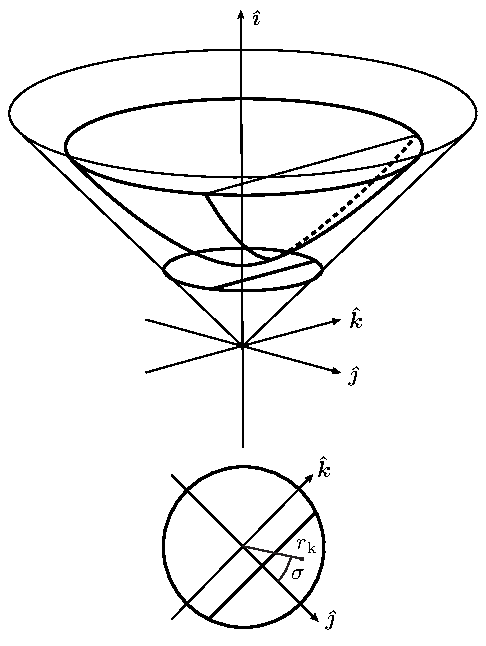
\includegraphics[scale=1]{media/other/cayley_disk-eps-converted-to}
    \caption{The Cayley-Klein disk and the hyperboloid model are related through gnomonic projection. A geodesic of on the hyperboloid model is shown as well, its projected image in the Cayley-Klein disk (also a geodesic) is a straight line. Illustration adapted from \citet{Balazs1986}.}
    \label{fig:cayley_disk}
\end{figure}

\paragraph{Poincaré disk} The \emph{Poincaré disk} is the image of the positive hyperboloid sheet under \emph{stereographic projection} with respect to the point $-\quati$, i.e. the point in Lorentzian 3-space with coordinates $(-1, 0, 0)$. This is illustrated in \cref{fig:poincare_disk} and \cref{fig:hyperboloid_projection}. If polar coordinates are used in the Poincaré disk, then the Euclidean rotation remains identitical, and the radial coordinate is equal to
\begin{equation} 
    r_\text{pc} = \tanh(\frac{\tau}{2}) = \frac{\sinh(\tau)}{1 + \cosh(\tau)}. 
\end{equation}
Because stereographic projection projects each point on the positive hyperboloid uniquely onto the Poincaré disk, every point on the disk corresponds to two possible elliptic trajectories: one with clockwise and one with counterclockwise rotation.

\begin{figure}[ht!]
    \centering
    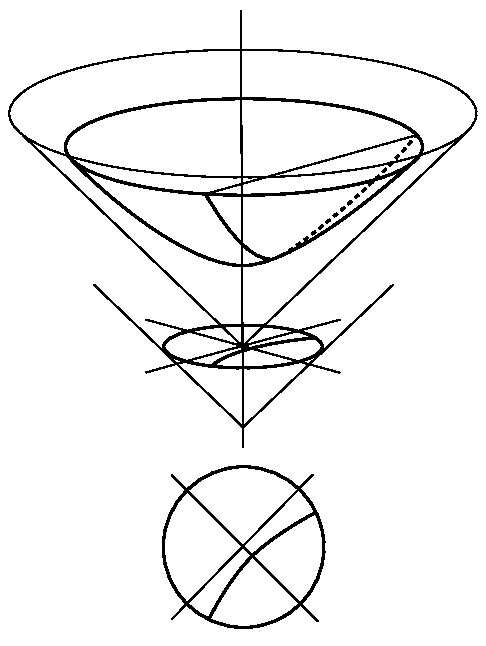
\includegraphics[scale=1]{media/other/poincare_disk-eps-converted-to}
    \caption{The Poincaré disk and the hyperboloid model are related through stereographic projection. A geodesic of on the hyperboloid model is shown as well, its projected image in the Poincaré disk (also a geodesic) is part of a circle that intersects the boundary of the disk at right angles. Illustration adapted from \citet{Balazs1986}.}
    \label{fig:poincare_disk}
\end{figure}


\subsubsection{Critically damped systems}

\subsubsection{Overdamped systems damped systems}

\FloatBarrier
\section{Notes}
! orthogonal refers to `regular' orthogonal, Lorentz-orthogonal makes the distinction.

Motivation: $\vec{u}$ seems to be `aligned' with major direction of the elliptic trajectory in the Lorentz-orthogonal subspace, generated by the action of its cross-product. Show this formally by making use of the eigenvectors.

The basis vectors $ \qty{\vec{e}_2, \vec{e}_3}$, where $\vec{e}_2$ is the orthogonal projection of the vector $\vec{e}_1 = \uvec{u}$ on its Lorentz-orthogonal subspace, and $\vec{e}_3 \triangleq \lorcrossp{\vec{e}_1}{\vec{e}_2}$, form the real and imaginary parts of two of the eigenvectors of the matrix $\mat{U}_{\lorcrossp{}{}}$. 

Because the basis vectors $\vec{e}_2$ and $\vec{e}_3$ are also orthogonal in the Euclidean sense, the 

\begin{proof}
    Let $\uvec{u} = u_1\uvec{i} + u_2\uvec{j} + u_3\uvec{k}$. A normal vector to the Lorentz-orthogonal subspace is $
    \uvec{n} = u_1\uvec{i} - u_2\uvec{j} - u_3\uvec{k}$. Then, the basis vectors are
    \begin{equation}
        \begin{split}
            \vec{e}_2 &= 
            \uvec{u} - \frac{ \inner{\uvec{u}}{\uvec{n}} }{ \inner{\uvec{n}}{\uvec{n}} } \uvec{n} \\
            \vec{e}_3 &= \lorcrossp{\uvec{u}}{\vec{e}_2} = -\frac{ \inner{\uvec{u}}{\uvec{n}} }{ \inner{\uvec{n}}{\uvec{n}} } \qty(\lorcrossp{\uvec{u}}{\uvec{n}}),
        \end{split}
    \end{equation}
    because the Lorentz-cross product distributes over addition and $\lorcrossp{\uvec{u}}{\uvec{u}} = \vec{0}$. The proposition above claims that $\vec{e}_2 + \ii\vec{e}_3$ is an eigenvector of the matrix $\mat{U}_{\lorcrossp{}{}}$. Hence, it must be the case that $\mat{U}_{\lorcrossp{}{}}(\vec{e}_2 + \ii\vec{e}_3) = \lambda(\vec{e}_2 + \ii\vec{e}_3)$, where $\lambda$ is then an eigenvalue of the matrix. This can be verified by replacing the action of $\mat{U}_{\lorcrossp{}{}}$ with the cross product. Plugging in the definition and exploiting the linearity of the Lorentz cross-product, we obtain:
    \begin{equation*}
        \begin{split}
            \lorcrossp{\uvec{u}}{\qty(\vec{e}_2 + \ii\vec{e}_3)} 
            &= \lorcrossp{\uvec{u}}{\vec{e}_2} +
        \ii\qty(\lorcrossp{\uvec{u}}{\vec{e}_3}) \\
            &= \vec{e}_3 + \qty(\lorcrossp{\uvec{u}}{\vec{e}_3})\ii \\ 
            &=\vec{e}_3 +  \qty(\lorcrossp{\uvec{u}}{\qty(\lorcrossp{\uvec{u}}{\vec{e}_2})})\ii \\
            &=\vec{e}_3 -  \frac{ \inner{\uvec{u}}{\uvec{n}} }{ \inner{\uvec{n}}{\uvec{n}} }\qty(\lorcrossp{\uvec{u}}{\qty(\lorcrossp{\uvec{u}}{\uvec{n}})})\ii.  \\
        \end{split}
    \end{equation*}
The triple cross-product expansion, or `Lagrange formula', relates the regular cross product to the corresponding dot product:
    $$ \vec{a}\times\qty(\vec{b}\times\vec{c}) = \vec{b}\:\inner{\vec{c}}{\vec{a}} - \vec{c}\:\inner{\vec{a}}{\vec{b}}. $$
This well-known identity generalizes (easily verified) to the Lorentzian counterpart of the cross- and inner products:
    $$ 
        \lorcrossp{\vec{a}}{\qty(\lorcrossp{\vec{b}}{\vec{c}})} 
       = \vec{b}\:\lorinner{\vec{c}}{\vec{a}} - \vec{c}\:\lorinner{\vec{a}}{\vec{b}}. 
    $$
Using the Lagrange formula, the above expression becomes
    \begin{equation*}
        \begin{split}
            & \vec{e}_3 - \frac{ \inner{\uvec{u}}{\uvec{n}} }{ \inner{\uvec{n}}{\uvec{n}} }\qty(\uvec{u}\,\lorinner{\uvec{u}}{\uvec{n}} - \uvec{n}\lorinner{\uvec{u}}{\uvec{u}})\ii \\
            & =\, \vec{e}_3 - \qty(\uvec{u}\,\frac{ \lorinner{\uvec{u}}{\uvec{n}} \, \inner{\uvec{u}}{\uvec{n}} }{ \inner{\uvec{n}}{\uvec{n}} } - \uvec{n}\frac{ \inner{\uvec{u}}{\uvec{n}} }{ \inner{\uvec{n}}{\uvec{n}} })\ii \\
            & =\, \vec{e}_3 - \qty(\uvec{u} - \uvec{n}\frac{ \inner{\uvec{u}}{\uvec{n}} }{ \inner{\uvec{n}}{\uvec{n}} })\ii \\
            & =\, \vec{e}_3 - \vec{e}_2\ii. 
        \end{split}
    \end{equation*}
    The latter is the scalar multiple of the vector $\vec{e}_2 + \vec{e}_3$ by $-\ii$ - hence, this is indeed an eigenvector of the corresponding matrix.
\end{proof}
Because $\vec{e}_2$ and $\vec{e}_3$ are also orthogonal in the normal sense, they are aligned with the major axes of the elliptic trajectories generated by the cross product. Hence, they can be used to find a basis of the invariant subspace which makes the trajectories identical to those in the phase plane.

\subsection{Relation with complex Hamiltonians}
\label{ssec:complex_ham}
